% This template was written by John Davies <john.davies@glasgow.ac.uk> 2017-02-06
% It matches the university specification at the time of writing
%   for the widths of the page margins and one-and-a-half line spacing
% You may want to include more packages, particularly for heavy mathematics
% Please let me know if you find any errors or wish to suggest improvements

\documentclass[12pt,titlepage,oneside]{book}
\usepackage[T1]{fontenc} % modern encoding
% Comment out the next three lines of LaTeX if you wish to use Computer Modern fonts
%   (this is the default for LaTeX)
% Make sure that your TeX installation can produce good pdf with these fonts.
% The following three lines are a good alternative if you don't use much mathematics
%\usepackage{mathptmx}  % uses Times for text and mathematics
%\usepackage[scaled]{helvet} %  helvetica for sanserif, scaled 95% by default
%\usepackage{courier}  % courier for typewriter font, pretty ugly but available
% otherwise the stix package offers more options and symbols
% \usepackage{stix}  % uses Times for text and a range of fonts for mathematics
% End of choices for fonts
\usepackage{graphicx}  % standard package for importing graphics files
%\usepackage{cite}  % improves format of numerical citations, such as [1-3]
\usepackage[top=1.8cm, bottom=1.8cm,left=4.0cm,right=1.5cm]{geometry}
% These margins are the university guidelines
\usepackage[onehalfspacing]{setspace}  % gives one-and-a-half line spacing
% doublespacing is another option and can be changed in the text
\usepackage{xcolor}
\definecolor{linkblue}{HTML}{335c97}
\usepackage[]{hyperref}
\hypersetup{
    colorlinks=True,
    linkcolor=linkblue,
}
\usepackage{dcolumn}   % needed for some tables
\usepackage{bm}        % for math
\usepackage{amssymb}   % for math
\usepackage{amsmath}   % for math
\usepackage{color}     % for colors

% packages for acronyms/glossary
%\usepackage{acronym}
\usepackage[toc,acronym]{glossaries}
%\renewcommand*{\glstextformat}[1]{\textsf{#1}}

% Chapter quotes
%\usepackage{epigraph}
%\setlength\epigraphwidth{8cm}
%\setlength\epigraphrule{0pt}


\usepackage{algcompatible} % algorithms
\usepackage{newfloat}
\usepackage{cancel}
\usepackage{tikz}
\usepackage{rotating}
\usetikzlibrary{shadows,arrows,arrows.meta,positioning,backgrounds,fit,chains,scopes}
\usepackage{subcaption}
\graphicspath{{./figures/}}
\usepackage{sidecap}

% setup for biber
\usepackage[
    backend=biber,
    style=numeric,
    natbib=true,
    url=true, 
    doi=true,
    eprint=false,
    sorting=none
]{biblatex}
\addbibresource{references.bib}

% some math operators
\DeclareMathOperator*{\argmin}{argmin}
\DeclareMathOperator*{\argmax}{argmax}

% pseudocode section
\DeclareFloatingEnvironment[
fileext=loa,
listname=List of Algorithms,
name=ALGORITHM,
placement=tbhp,
]{algorithm}


\sidecaptionvpos{figure}{c}



\newcommand{\joe}[1]{\textbf{\textcolor{blue}{JOE: #1}}}
\newcommand{\graham}[1]{\textbf{\textcolor{red}{GRAHAM: #1}}}
\newcommand{\chris}[1]{\textbf{\textcolor{green}{CHRIS: #1}}}

%\usepackage{charter}
%\usepackage[expert]{mathdesign}


\makeglossaries

\newacronym{GW}{GW}{gravitational-wave}
\newacronym{GR}{GR}{general relativity}
\newacronym{GRB}{GRB}{gamma ray burst}
\newacronym{CW}{CW}{continuous gravitational wave}
\newacronym{CBC}{CBC}{compact binary coalescence}
\newacronym{BBH}{BBH}{binary black hole}
\newacronym{BNS}{BNS}{binary neutron star}
\newacronym{NSBH}{NSBH}{neutron star black hole}
\newacronym{EMRI}{EMRI}{extreme mass ratio inspiral}
\newacronym{NS}{NS}{neutron star}
\newacronym{EOS}{EOS}{equation of state}
\newacronym{EM}{EM}{electromagnetic}
\newacronym{SNR}{SNR}{signal-to-noise-ratio}
\newacronym{LIGO}{LIGO}{Laser Interferometer Gravitational-wave Observatory}
\newacronym{SFT}{SFT}{short Fourier transform}
\newacronym{FFT}{FFT}{fast Fourier transform}
\newacronym{UCD}{UCD}{up, centre or down}
\newacronym{MDC}{MDC}{mock data challenge}
\newacronym{PSD}{PSD}{power spectral density}
\newacronym{ROC}{ROC}{receiver operating characteristic}
\newacronym{RMS}{RMS}{root median square}
\newacronym{MCMC}{MCMC}{Markov-Chain Monte Carlo}
\newacronym{SOAP}{SOAP}{snakes on a plane}
\newacronym{CNN}{CNN}{convolutional neural network}
\newacronym{CMB}{CMB}{cosmic microwave background}
\newacronym{LISA}{LISA}{laser interferometer space antenna}
\newacronym{PEM}{PEM}{physical environment monitor}
\newacronym{CFS}{CFS}{Chandrasekhar, Friedman and Schutz}
\newacronym{SSB}{SSB}{solar system barycenter}
\newacronym{MSU}{MSU}{million standard units}
\newacronym{ASD}{ASD}{amplitude spectral density}
\newacronym{CPU}{CPU}{central processing unit}
\newacronym{GPU}{GPU}{graphics processing unit}
\newacronym{USA}{USA}{united states of America}
\newacronym{NoEMi}{NoEMi}{noise frequency event miner}
\newacronym{CR}{CR}{critical ratio}
\newacronym{SGWB}{SGWB}{stochastic gravitational wave background}

\begin{document}
\begin{titlepage}
\centering
\vspace*{3cm}  % Need the * or the space is swallowed at the top of the page
\bfseries\Large
Data Analysis Techniques for Continuous Gravitational Wave Searches\\
\vspace{3cm}
\normalfont\large
Joseph Bayley\\
\vspace{2cm}
Submitted in fulfilment of the requirements for the\\
Degree of Doctor of Philosophy\\
\vspace{2cm}
School of Physics and Astronomy\\
College of Science and Engineering\\
University of Glasgow\\
\vspace{1cm}

\includegraphics[scale=0.125]{GlaLogo.pdf}
\\
\vspace{1cm}
% Insert month and year of date deposited with library for final version
February 2017
\end{titlepage}
\frontmatter  % Turn off chapter numbering, use roman page numbers
\chapter{Abstract}

The field of gravitational wave astronomy is still in its early stages, with
detections of compact binary coalescences numbering $\sim
12$ and the most recent observing run (O3) providing $\sim 50$ more candidates. Another possible source of
gravitational waves is rapidly rotating neutron stars which can emit gravitational waves if they have some asymmetry
around their rotation axis.
These are predicted to emit long duration quasi-sinusoidal signals known as
continuous gravitational waves.

% SOAP chapter
All-sky and wide parameter space searches for continuous gravitational waves
are generally template-matching schemes which test a bank of signal waveforms
against data from a gravitational wave detector.  Often these searches  are highly-tuned to specific signal types and are computationally
expensive. We have developed a search method (entitled SOAP) based on the Viterbi
algorithm which is model-agnostic and has a computational cost several orders
of magnitude lower than template methods and with a comparable sensitivity. 
In particular, this method can search for
signals which have an unknown frequency evolution. We test the algorithm on
three simulated and real data sets: gapless Gaussian noise, Gaussian noise with
gaps and real data from the final run of initial LIGO (S6). We show that at
95\% efficiency, with a 1\% false alarm rate, the algorithm achieves a sensitivity of $\sim 60,\, 72$ and $74$ in the optimal coherent signal to noise ratio in each of these datasets.
We discuss the use of this algorithm for detecting a wide range of quasi-monochromatic
gravitational wave signals and instrumental artefacts, and
demonstrate that it can also identify shorter duration signals such as compact binary coalescences.


% Machine learning chapter
Many continuous gravitational wave searches are affected by instrumental lines
as the long duration narrowband nature of a line can appear to be very similar
to a real continuous gravitational wave signal.  This has led
to the development of techniques to try and limit the effect of
instrumental lines, which mostly involve developing a statistic to penalise
signals that appear in only a single detector.  
Whilst these statistics limit the effect of instrumental lines, in the SOAP search described above, many lines still contaminated the statistics and had to be manually removed by investigating other search outputs.
We have developed a method using convolutional neural networks to reduce the impact of instrumental
artefacts on the SOAP search described above.  This has the
ability to identify features in each detectors spectrograms such that a
frequency band can be classified into a signal or noise class.  
This limits the amount of manual investigation of bands and allowed the SOAP search to be fully automated without a reduction in the sensitivity.



% Parameter est chapter 
Once a continuous gravitational wave is detected, we would want to extract some
parameters associated with the source to help understand more about its
structure and evolution. We describe a Bayesian method which extracts the sky
location, frequency, frequency derivative and signal to noise ratio of a source associated with the
frequency evolution returned by the SOAP algorithm.  This has the aim of
limiting the size of the parameter space for a more sensitive fully coherent
follow up search.  
We tested this approach on 200 simulations in Gaussian noise, and in 90\% of these simulations we limit the sky area to 45 deg$^2$ with a 95\% confidence contour.
However, find that this contour contains the true parameter only 42\% of the time.
We present these results and describe the features and shortcomings of our approach.

~\chris{You maybe don't need to
be as bluntly negative and honest as you are here. I would advise slightly
expanding the description but also say that we present results and describe the
features and shortcomings of our approach. Or something like that. While we are
talimng about the PE, I would expect the results to be more presentable if you
take the 50\% confindence interval as opposed to the 95\%. Have you been bale
to do this yet?}

% Lines chapter
As mentioned above, we limit the effect of instrumental lines on the SOAP
search using machine learning, however we can also identify and mitigate these
lines separately before a search is run.  We demonstrate how we can use SOAP in
a simple configuration to identify instrumental lines.  We compare this method
to existing line identification tools used in the \gls{LIGO} collaboration, and
find that using the Viterbi statistic SOAP identifies $\sim 37$\% of the same lines as these methods, where of the lines which were not identified, other SOAP outputs do show evidence of a line.
With further investigation, we expect to identify many more lines in common with existing methods.
As well as these common lines, the SOAP algorithm returned $\sim 150$ more bands which potentially contain an instrumental line, which did not appear on \gls{LIGO} line-lists.









\glsunsetall
\tableofcontents
\listoftables
\listoffigures
\glsresetall
\chapter{Acknowledgements}


\chapter{Declaration}



\glossarystyle{listhypergroup}
\printglossaries
	


\mainmatter % Turn on chapter numbering, reset page numbers, use arabic
\chapter{\label{intro}Introduction}
%%%%%


\Glspl{GW} were first predicted in 1915 as a consequence of Einstein's general theory of relativity \citep{einstein2005GrundlageAllgemeinen}.
They are theorised as ripples in the fabric of space-time.
The first observational evidence that \glspl{GW} exist came from observations of the Hulse-Taylor binary \citep{weisberg1981GravitationalWaves,weisberg2004RelativisticBinary}. 
This observation of a pulsar in a binary system showed that the periastron was reached slightly early after each orbit, implying that the pulsars orbit was decreasing with time. 
If the separation of two orbiting objects is decreasing then the system must be losing energy.
The loss in energy matched the \gls{GR} prediction which assumed the energy was lost to \glspl{GW}.
This gave hope of \glspl{GW} existence and helped lead the way to designing instruments which could directly detect them.
The first direct detection of gravitational waves was made in 2015 when the two \gls{LIGO} detectors in the US \citep{abbott2016ObservationGravitational} identified a signal from a \gls{BBH} system.
This was not only the first observation of a \gls{GW} but gave information on a yet unobserved astrophysical system.
This has since been followed by many more detections of \gls{BBH} signals involving \gls{LIGO} and Virgo including \citep{abbott2017GW170814ThreeDetector,theligoscientificcollaboration2020GW190425Observation}.
In 2017 the \gls{LIGO} detectors observed the first \gls{BNS} system \citep{abbott2017GW170817Observation} which had a corresponding electromagnetic counterpart.
This allowed verification of the source from optical counterparts and started the era of multi-messenger astronomy.
These detections opened up the field of gravitational wave astronomy, where many more detections are expected to give more information on the universe and objects within it.

As well as searching for \gls{BBH} and \gls{BNS} signals, there are many efforts to detector other types of \gls{GW} signals. 
This thesis focuses on efforts to search for a particular type of \gls{GW} which are thought to originate from rapidly rotating neutron stars.
In chapters \ref{intro} and \ref{searchcw} I will review introductory material. 
This includes a general introduction to the generation of \glspl{GW} in Sec.~\ref{intro:gravwaves} and their sources in Sec.~\ref{intro:sources}.
I will then introduce instruments used to detect \gls{GW} in Sec.~\ref{intro:detector}.
In Chapter \ref{searchcw} I will introduce the general model for \glspl{CW} and current methods used to detect them.
Chapters \ref{soap}, \ref{machine} and \ref{detchar} will go into detail about techniques developed by the author to search for \gls{CW} signals. 
Finally I will summarise this work and discuss future developments in chapter \ref{summary}.


%%%%%%%%%%%
%%%%%%%%%
\section{\label{intro:gravwaves}Gravitational waves}
%%%%%%%%%%%
%%%%%%%%%

In general relativity, gravity is thought of as the curvature of space-time and matter moves according to this curvature. 
The matter in the universe also has an effect on the curvature of the space-time.
The larger the mass of matter the more the space-time is distorted.
Space-time can generally be described by Einstein's field equations
\begin{equation}
\label{intro:gravwaves:efe}
    G_{\mu \nu} = \frac{8 \pi G}{c^4}T_{\mu \nu}.
\end{equation}
where $G_{\mu \nu}$ is the Einstein tensor and $T_{\mu \nu}$ is the stress-energy tensor.
The stress energy tensor describes the mass-energy in the universe, where its components contain information on the density of energy and momentum.
The Einstein tensor contains information on the curvature of the universe. 
This can be derived directly from the metric tensor $g_{\mu \nu}$ which describes the geometry of the universe.
Einstein's equations then explain how the curvature of space-time changes with the mass-energy within it. 
In empty space one can assume that the geometry of space-time is flat, i.e. there is no curvature to space-time. The metric tensor for this can then be defined as
\begin{equation}
g_{\mu \nu} = \eta_{\mu \nu} = \left(
\begin{matrix}
-1 & 0 & 0 & 0 \\
0 & 1 & 0 & 0 \\
0 & 0 & 1 & 0 \\
0 & 0 & 0 & 1 
\end{matrix}
\right).
\end{equation}
Each index of this matrix refers to a space-time dimension, i.e. $x^0 = t$, $x^1=x$, $x^2=y$ and $x^3=z$. 
Measuring a distance $dx$ in space-time can be different for different observers, therefore, one needs a measure which is invariant for every observer. 
This is the space-time interval $ds$, also known as the line element, between two `events' in space-time. 
This is defined as
\begin{equation}
\label{intro:lineelement}
    ds^2 = g_{\mu \nu} dx^{\mu}dx^{\nu}.
\end{equation}
As in Einstein's notation this is a sum over the indices $\mu$ and $\nu$.  
Equation \ref{intro:lineelement} can be thought to describe the space-time `distance' between the two events.
For flat space-time, $\eta_{\mu\nu}$, this can then be written as
%
\begin{equation}
    ds^2 = -c^2 dt^2 + dx^2 + dy^2 + dz^2.
\end{equation}
%
The Einstein equations Eq.~\ref{intro:gravwaves:efe} then demonstrate how the curvature of space-time $G_{\mu\nu}$ depends on the matter and energy distribution $T_{\mu \nu}$ within it.

A gravitational wave can be described as a ripple in this space time.
The simplest way to visualise this is just a small time dependent change to the flat space-time metric $\eta_{\mu\nu}$.
In linearised theory of gravity, the space-time metric $g_{\mu \nu}$ can be defined as
\begin{equation}
\label{intro:gravwave:metric}
    g_{\mu \nu} = \eta_{\mu \nu} + h_{\mu \nu},
\end{equation}
where $ \eta_{\mu \nu}$ is the metric for flat space-time and $h_{\mu \nu}$ is some perturbation, where $|h_{\mu \nu}| \ll 1$ \citep{flanagan2005BasicsGravitational}. 
In this linearised theory the perturbations to the metric tensor are assumed to be small, therefore, Einstein's field equations can be solved such that the solution is a plane wave. 
More information on this derivation can be found in \citep{flanagan2005BasicsGravitational,letiec2016TheoryGravitational}.
By using $g_{\mu \nu}$ from Eq.~\ref{intro:gravwave:metric}, we can write the linearised Einstein equations as
\begin{equation}
\label{intro:lineinstein}
    \Box h_{\mu \nu} = -16 \pi T_{\mu\nu},
\end{equation}
where $\Box$ is the d'Alembert operator which in flat space is defined by
\begin{equation}
		\Box = -\frac{1}{c^2} \frac{\partial^2}{\partial t^2} + \frac{\partial^2}{\partial x^2} + \frac{\partial^2}{\partial y^2} + \frac{\partial^2}{\partial z^2}
\end{equation}
In empty space there is no matter, therefore, all the components of the stress energy tensor  are zero, i.e. $T_{\mu \nu} = 0$.
This allows Eq.~\ref{intro:lineinstein} to be reduced to
\begin{equation}
    \Box h_{\mu \nu} = 0,
\end{equation}
Which is of course the wave equation. 
This follows the same form as in electrodynamics and the general plane-wave solutions have the form
\begin{equation}
    h_{\mu\nu} = A_{\mu\nu}e^{ik_{\alpha} x^{\alpha}},
\end{equation}
where each component of $h_{\mu \nu}$ is a sinusoid traveling along vector $k_{\alpha}$ with amplitude $A_{\mu\nu}$ \citep{capano2011SearchingGravitational}.
At this point the set of equations are not simple; the symmetric tensor $A_{\mu \nu}$ has 10 independent components.
This can be greatly simplified by choosing a different gauge where the metric perturbation is both transverse and traceless (TT) \citep{flanagan2005BasicsGravitational}.
This is just a choice of coordinate system which does not change any current assumptions \joe{read more about gauges}. A traceless metric is one where the sum of the diagonal elements are 0 and a transverse metric is when the oscillations are perpendicular to the direction of travel. 
This gauge imposes two conditions: one is that $h_{\mu \nu}$ is traceless, i.e. that the sum of the diagonal elements are 0 and the other is that $h_{\mu \nu}$ is transverse. 
The transverse element means that the oscillations of the wave happen perpendicular to the direction of travel.
At this point we can choose that the wave is traveling in the $z$ direction which means that $k = (\omega,0,0,k)$.
By then adopting the TT gauge there are only two unique components to the metric such that the perturbation is
\begin{equation}
\label{intro:gw:gravwave}
h_{\mu \nu} = \left( 
\begin{matrix}
0 & 0 & 0 & 0 \\
0 & h_{+} & h_{\times} & 0 \\
0 & h_{\times} & -h_{+} & 0 \\
0 & 0 & 0 & 1 \\
\end{matrix}
\right) 
e^{i(kt - wt)}.
\end{equation}
The two unique components are then the two polarisations of gravitational waves, $h_{+}$ and $h_{\times}$.
The affect of each of the polarisations on a ring of test particles can be seen in Fig.~\ref{gw:polarisations} where the gravitational wave is travelling out of the page.

\begin{figure}[h]
    \centering
    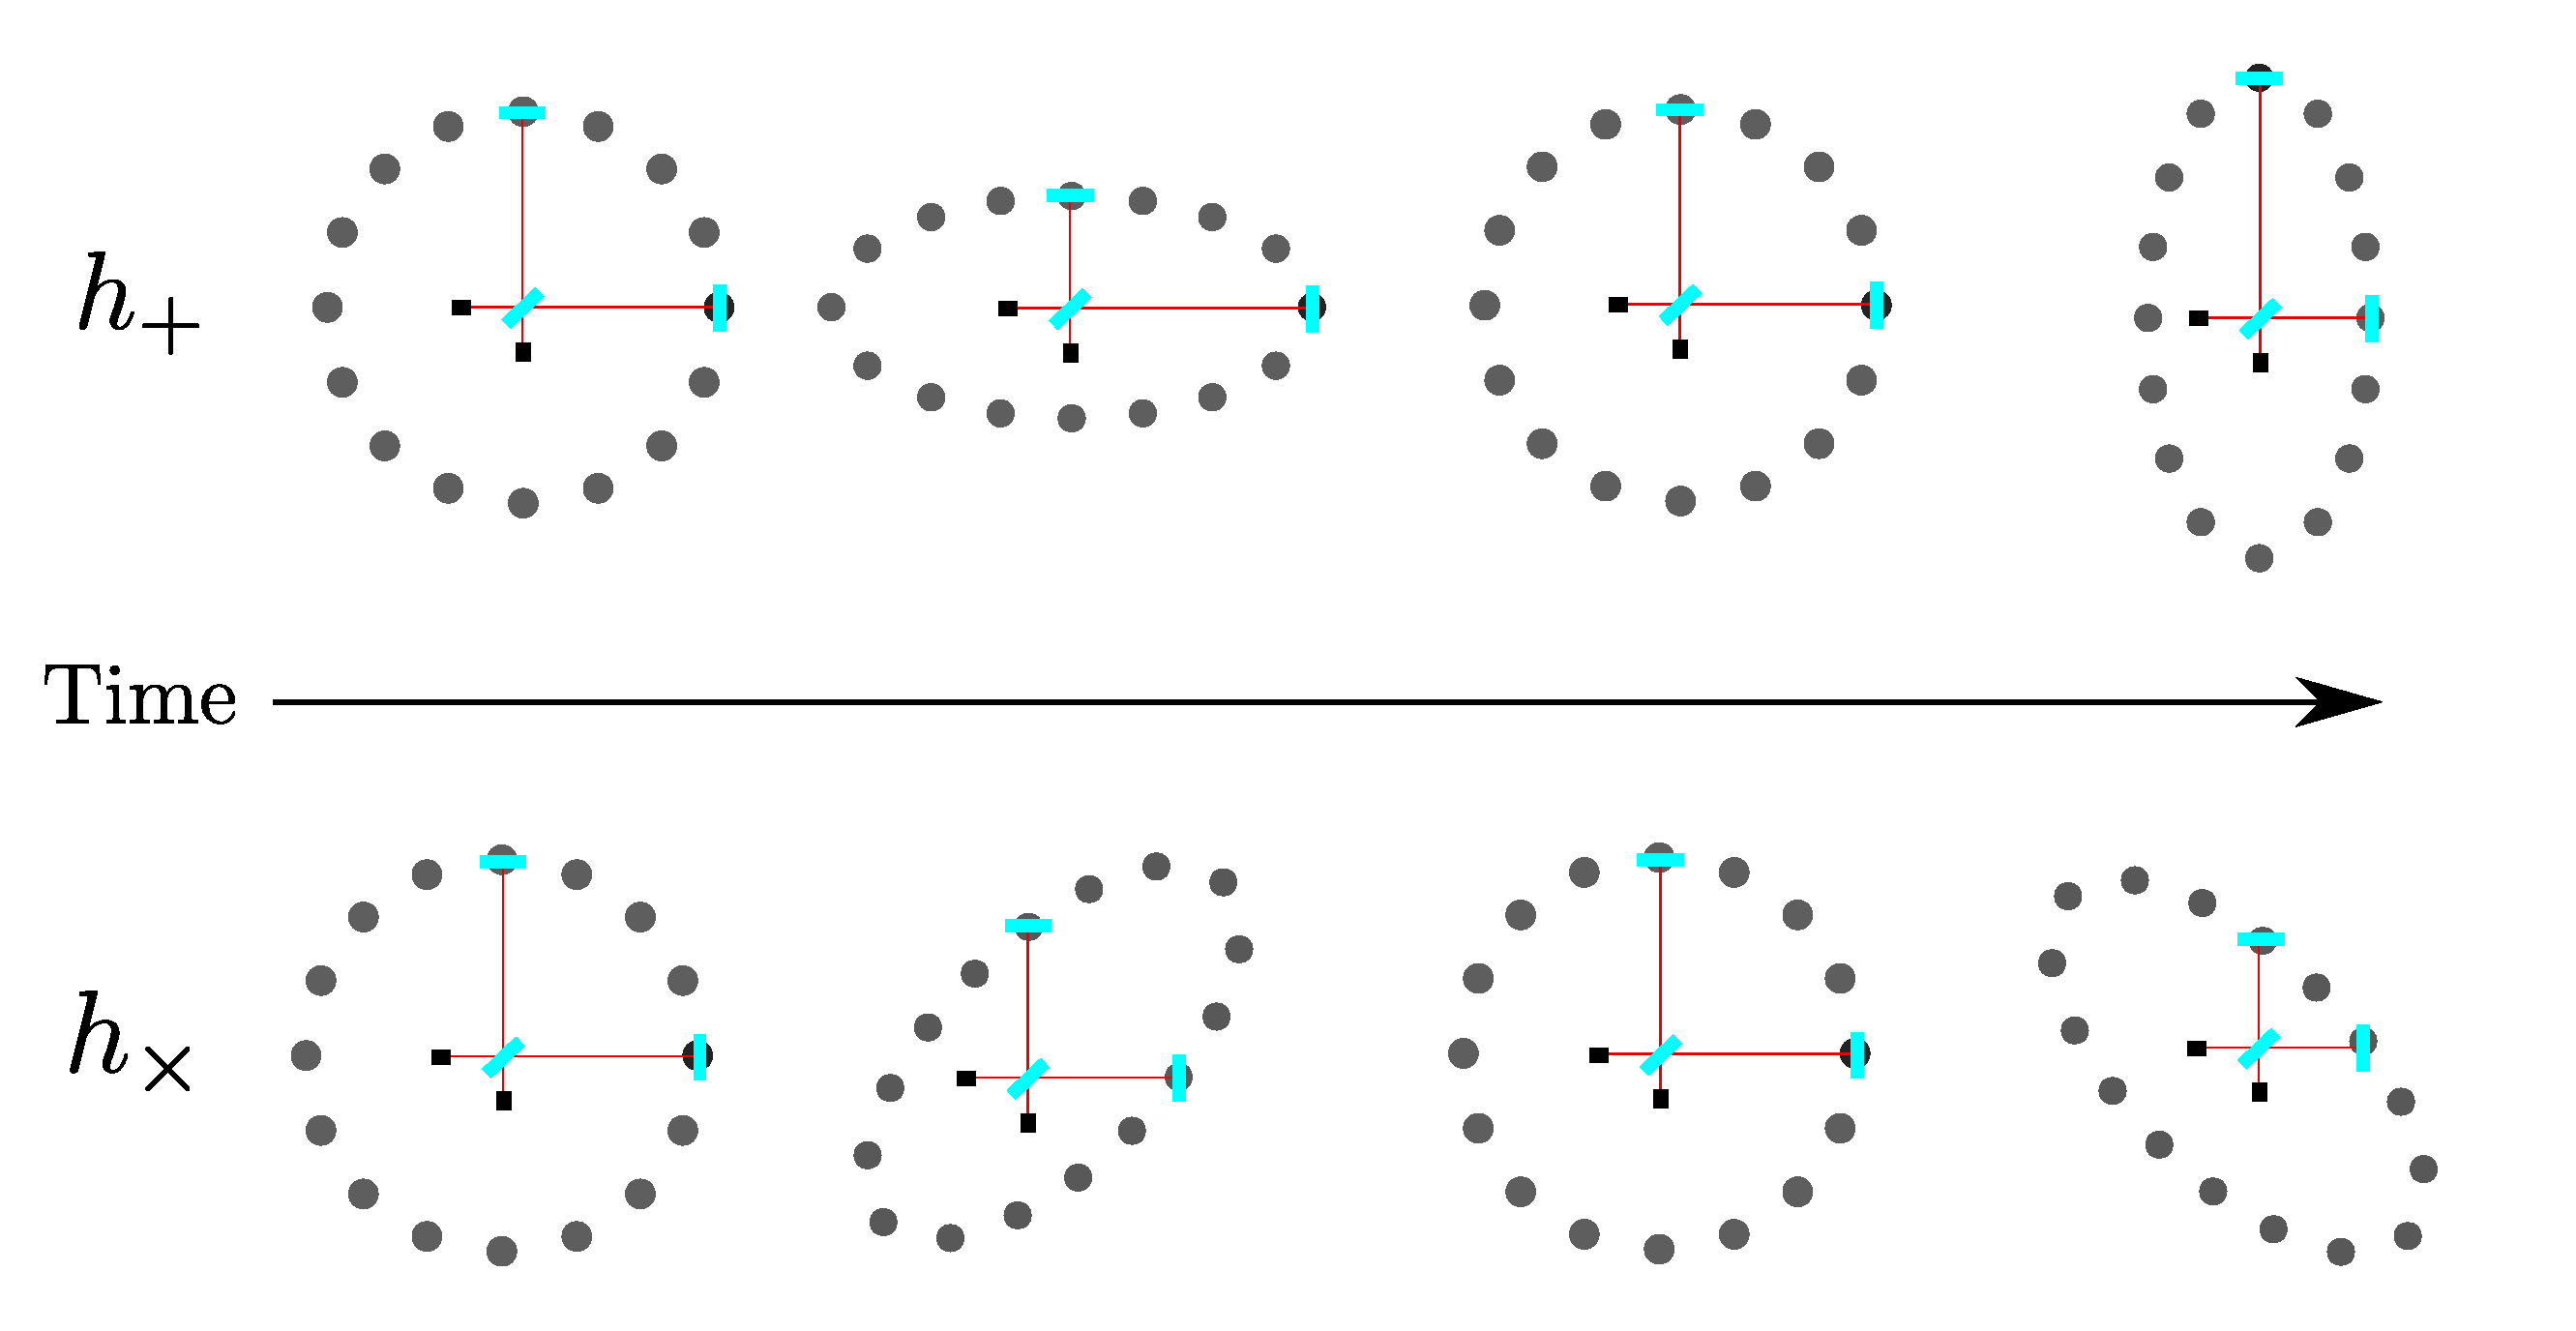
\includegraphics[width=\textwidth]{C1_intro/polarisation_ring.pdf}
    \caption[Plus and Cross polarisations]{Shows how the plus and cross polarisations affect a ring of test particles. This assumes the wave is travelling out of the page and the effects have been greatly exaggerated. This also shows an example of how this effects the test masses of an interferometer. This will be described in more detail in Sec.~\ref{intro:detector}.}
    \label{gw:polarisations}
\end{figure}



\subsubsection{Generating gravitational waves}

To generate gravitational waves we go back to Eq.~\ref{intro:lineinstein} where we include the stress-energy term on the right hand side.
Following the derivation in \citep{flanagan2005BasicsGravitational}, one can find that the gravitational wave amplitude is related to the second moment of the mass distribution.
The second moment of the mass distribution $I_{\mu\nu}$is defined as
\begin{equation}
    I_{\mu \nu}(t) = \int \rho(t,{\bf x}) x^\mu x^\nu d^3x,
\end{equation}
where $\rho$ is the mass density, and $x_i$ and $x_j$ are the coordinates \citep{flanagan2005BasicsGravitational}. 
This is the quadrupole moment tensor without the trace subtracted.
The gravitational wave amplitude is then
\begin{equation}
\label{intro:gravwave:amp}
    h_{\mu \nu} = \frac{2}{r}  \frac{d^2 I_{\mu \nu}(t-r)}{dt^2},
\end{equation}
where $r$ is the distance from the source \citep{letiec2016TheoryGravitational}.
This has a slight modification in the TT gauge, see \citep{flanagan2005BasicsGravitational}, however, has the same relationship between the mass quadrupole and the \gls{GW} amplitude.
This shows that for a \gls{GW} to be generated, the second derivative of the mass quadrupole moment is needed.
A mass quadrupole moment only exists when the mass distribution is not spherically symmetric.
Therefore, a mass which is asymmetric and accelerating will produce a \gls{GW}.

Systems which will produce detectable \glspl{GW} are generally rapidly rotating high mass systems which have some asymmetry around their rotation axis.
The sources of these \gls{GW} will be described in the following section.



%%%%%%%%%%%%%%
%%%%%%%%%%%%%
\section{\label{intro:sources}Sources and signals}
%%%%%%%%%%%%%%%
%%%%%%%%%%%%%%%

There are many potential sources for \gls{GW}. The expected sources can be split into 3 general categories based on their signal type: Transient, Stochastic and \glspl{CW}.
These categories are chosen based on the length of the signal and how well modelled the signal is.
Figure \ref{intro:sources:signaltypes} shows an example of each of the signals and their category.
%
\begin{figure}[h]
    \centering
    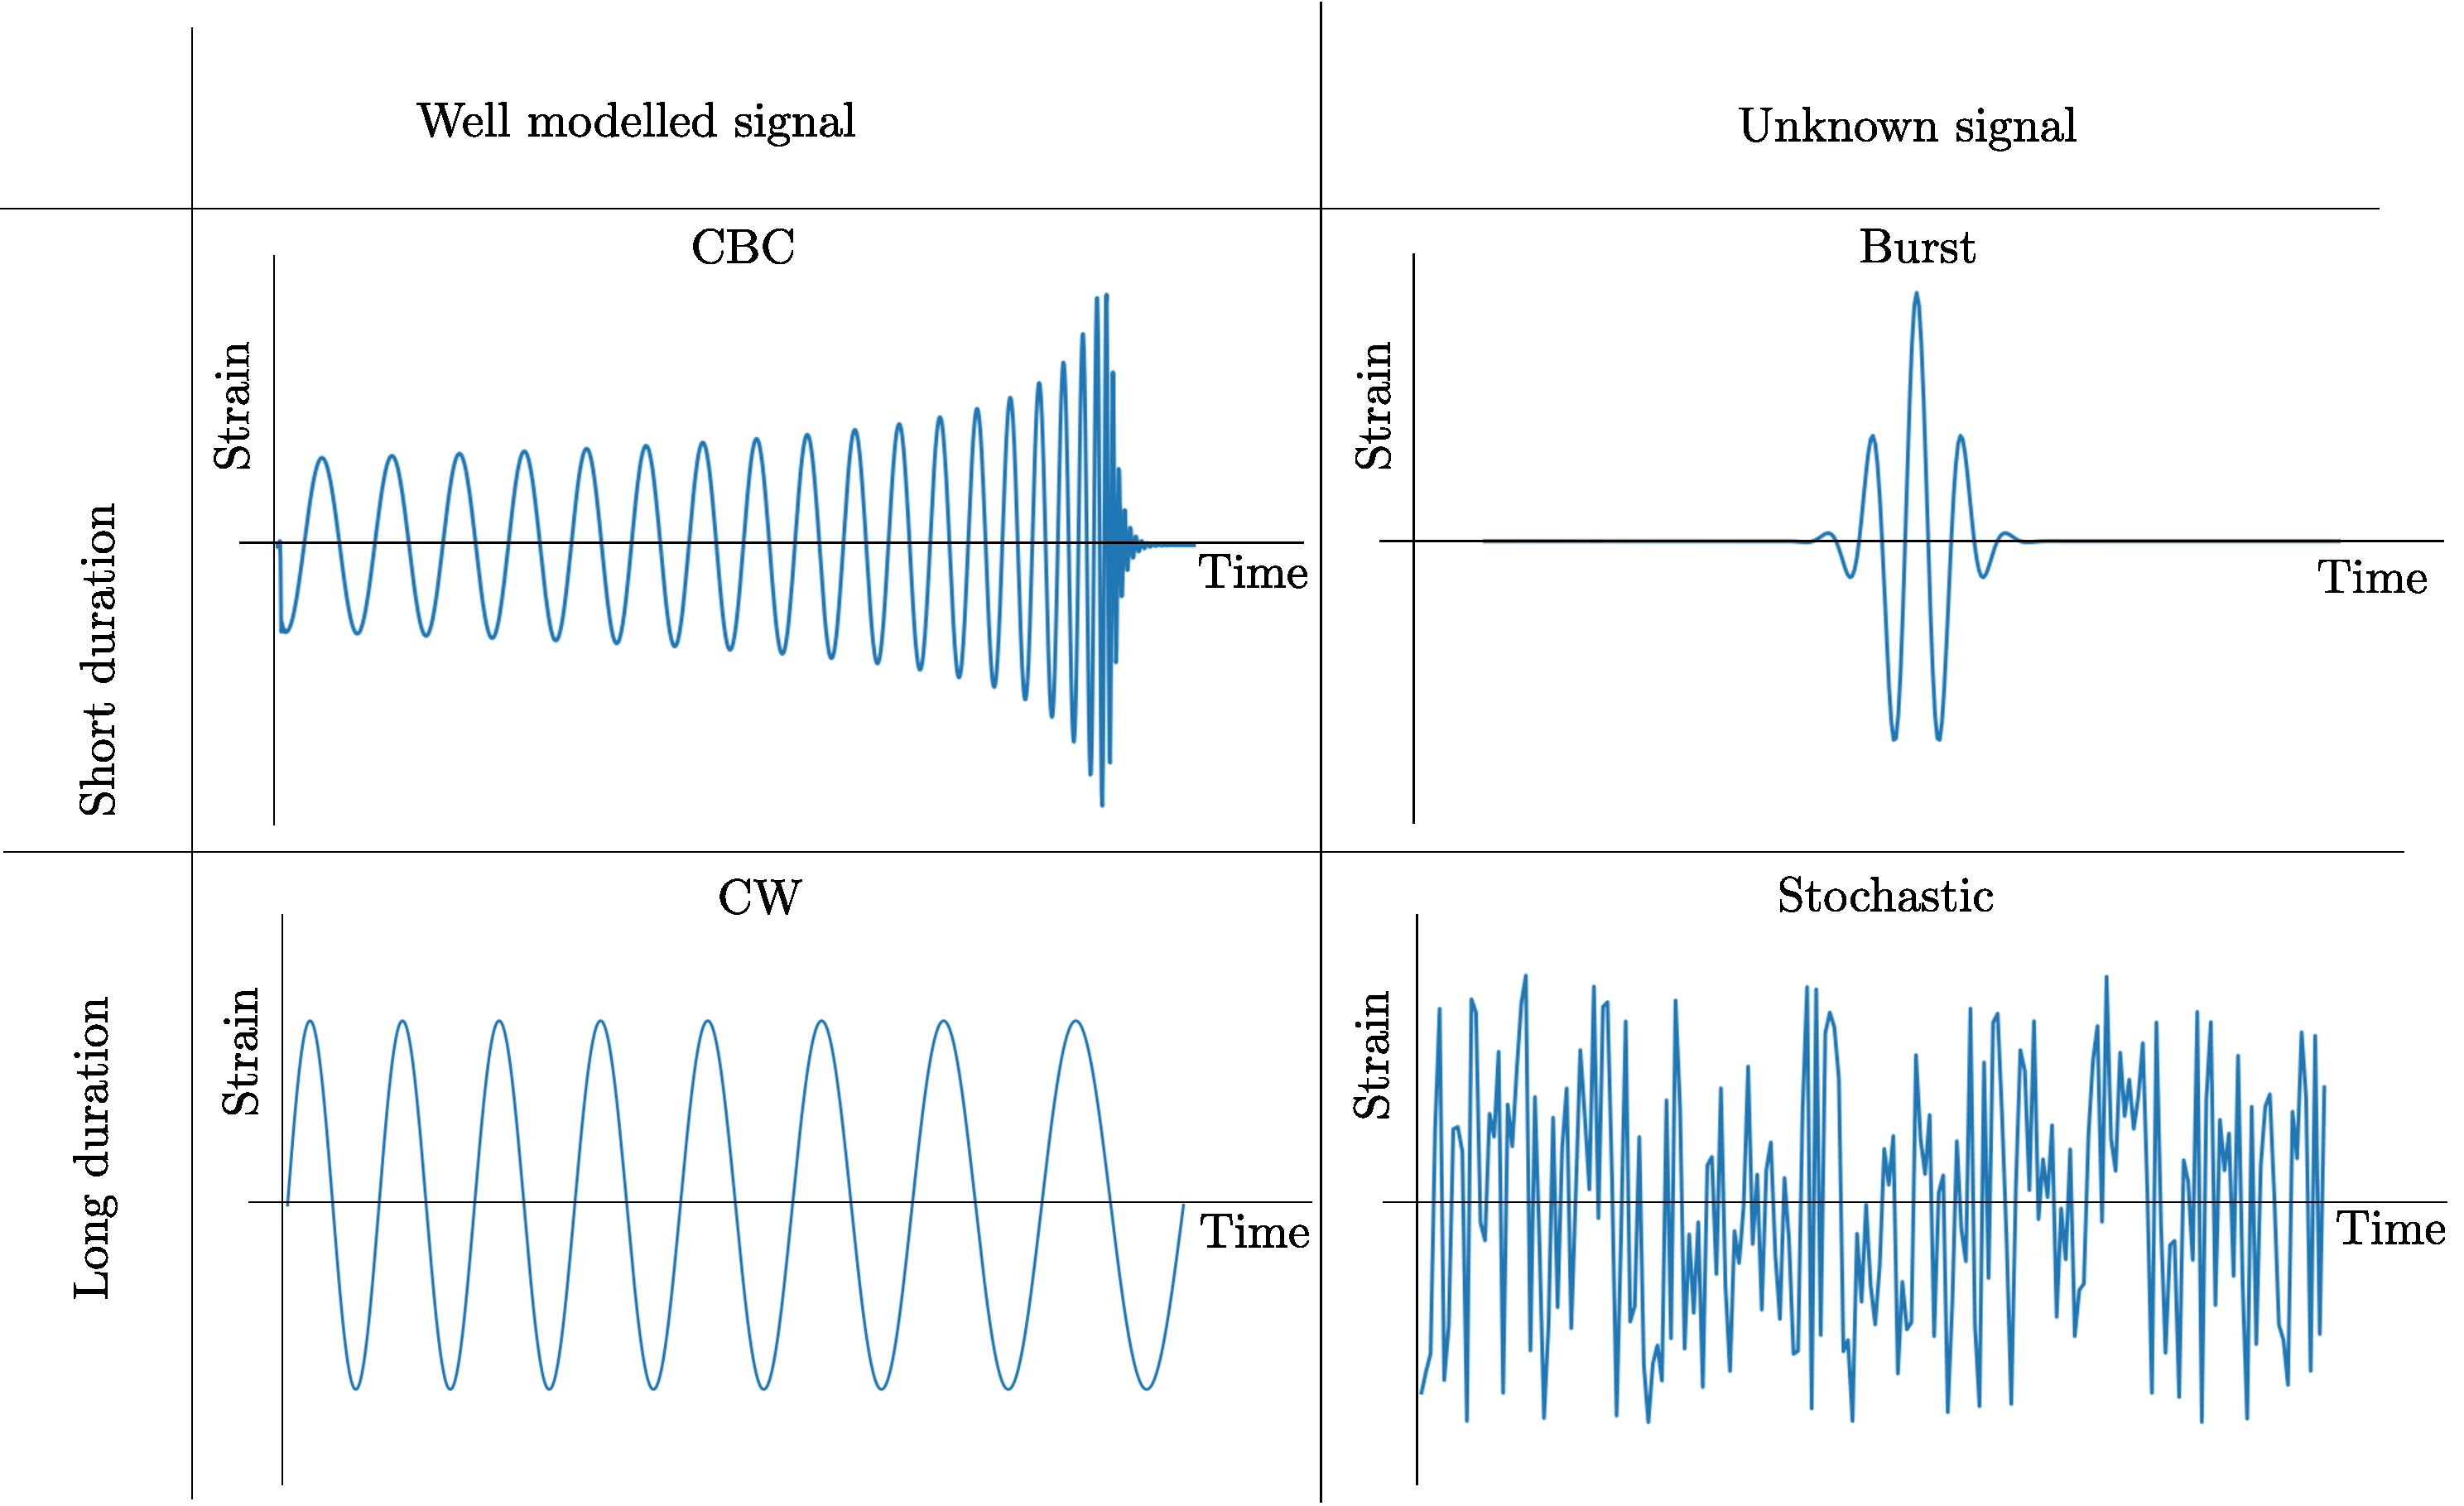
\includegraphics[width=\textwidth]{C1_intro/sources_types.pdf}
    \caption[GW signal types]{Each \gls{GW} signal type can be categorised based on its signal length and how well the signal is modelled. Transient signals which are short duration in the ground based detectors band, include both well modelled \gls{CBC} signals and unknown Burst signals. Long duration signals include well modelled \gls{CW} signals and unknown Stochastic signals.}
    \label{intro:sources:signaltypes}
\end{figure}
In the sections that follow, I will give an overview of the potential sources of each of these signal categories and their wave-forms.


%%%%%%%%%%%%%%%
\subsection{\label{sources:transient} Transient}
%%%%%%%%%%%%%%%

Transient sources of \glspl{GW} are short duration signals which are, depending on the source, observable from milliseconds to tens of seconds in current ground based detectors frequency band. 
Some of these sources, particularly \gls{CBC} sources, will emit signals for a much longer time, however these are at a lower frequency and not observable by current ground based detectors detectors.
Transient signals can be further split into two categories based on how well they are modelled. 
\glspl{CBC} have well modelled wave-forms and bursts are generally from un-modelled or unknown sources.

\subsubsection{\label{sources:transient:cbc} Compact Binary Coalescence}

\glspl{CBC} originate from the in-spiral and merge of two compact objects which are gravitationally bound.
The objects inspiral as they lost energy to the radiation of gravitational waves.
Dependent on the masses and distances of the two objects, the gravitational waves generated by the system can be detected by ground based detector such as LIGO \citep{aasi2015AdvancedLIGO} and Virgo \citep{acernese2015AdvancedVirgo}. 
In fact, the only detections to date have been of this type; these are summarised in \citep{ligoscientificcollaborationandvirgocollaboration2019GWTC1GravitationalWave}.

\joe{More qualatative, See Grahams comment}
The compact objects referred to here are either either black holes or neutron stars.
There are generally three types of \gls{CBC} source: \gls{BBH}, \gls{BNS} and \gls{NSBH}.
The general structure of the waveform is the same for each of these and follows a `chirp' where the \gls{GW} frequency increases with time until merger. An example of this is shown in Fig.~\ref{intro:sources:signaltypes}.
For higher mass systems such as \gls{BBH} these signals are detectable by ground based detectors for $< 1\,s$. 
For lower mass systems such as \gls{BNS} they can be detected for longer periods $\mathcal{O}(10)$s. 
The lower frequency parts of the signal (i.e. earlier times) aim to be detected by future space based detectors such as \gls{LISA} \citep{danzmann1996LISALaser}.

In systems which have a neutron star, during the in-spiral and merger phase, the neutron star can deform due tidal interactions between the objects \citep{flanagan2008ConstrainingNeutronstar}. 
This becomes useful as it will affect the generated waveform and can help place limits on and determine the \gls{EOS} for the dense matter in a neutron star \citep{harry2018ObservingMeasuring}. %\citep{hernandezvivanco2019MeasuringNeutron}
\gls{BNS} systems also offer a way do observe objects in multiple different channels, or what is known as multi-messenger astronomy. 
This is where the object can be viewed in the \gls{EM} spectrum as well as in gravitational waves.
This offers much in the field of astronomy as it can aid in the measurement of the Hubble constant \citep{theligoscientificcollaborationandthevirgocollaboration2017GravitationalwaveStandard}. 
Observations of \gls{BBH} systems can also give information on how black holes and \glspl{BBH} form, more details on this can be found in \citep{zevin2017ConstrainingFormation,mandel2018MergingStellarmass}.


%%%%%%%%%%%%%%
\subsubsection{\label{sources:transient:burst}Burst}
%%%%%%%%%%%%%%%%%

Burst sources are also short duration however, are un-modelled or difficult to model, in the sense that the exact waveform of the signal is unknown.
There are two possible reasons for the lack in knowledge of the waveform: the physics of the system is too complicated to model in a reasonable amount of time or there is no model of the source.
As there is no model to generate waveforms, burst searches cannot use matched filtering as in \gls{CBC} searches.
Rather burst searches look for short bursts in power which is coincident between multiple detectors \citep{cornish2015BayeswaveBayesian, klimenko2008CoherentMethod}.
There are a number of systems which could potentially emit a short duration burst signals.
These include core collapse supernovae \citep{ott2008GravitationalWave}, \glspl{GRB} \citep{aasi2014SearchGravitational}, cosmic strings \citep{damour2005GravitationalRadiation} and other unknown sources.
Detecting \gls{GW} from one of these sources could offer more insight into the processes which cause core collapse supernovae. 

As burst searches are un-modelled, they are sensitive to almost any signal which is coherent between detectors. 
This allows them to also search for signals from \gls{CBC} as well as any \gls{GW} signal from an unknown source.



%%%%%%%%%%%%%%%
\subsection{Stochastic}
%%%%%%%%%%%%%%%

The stochastic background has no signal model, however, is expected to be a persistent source of \gls{GW} in the background of the detector. 
The stochastic background is the incoherent sum of many unresolved \gls{GW} signals.
The source of these signals can be anything from cosmological sources such as cosmic strings to \gls{CBC} signals.
These signals can be thought of as the \gls{GW} analogue of the \gls{CMB}.
The signal is assumed to be isotropic such that it can be observed at any point on the sky \citep{christensen2018StochasticGravitational}. 
As the stochastic background is noise-like it is very difficult to distinguish from noise within a single detector \citep{christensen2018StochasticGravitational}.
Therefore, searches for the stochastic background correlate signals between multiple detectors \citep{romano2019SearchesStochastic,christensen2018StochasticGravitational}. 
When detected, these signals may be able to offer insights into the early universe and its formation.



%%%%%%%%%%%%%%%%%%
\subsection{\label{intro:sources:cw}Continuous waves}
%%%%%%%%%%%%%%%%%%%%

\glspl{CW} are long duration signals which can be well modelled.
The signals last for times greater than the observation runs of ground based detectors and in general have a fixed or slowly varying frequency.
There are a number or potential sources of \glspl{CW} including a \gls{CBC} signal earlier in the inspiral phase.
Before the final stages of the inspiral of a \gls{CBC} signal, the objects orbiting at much slower non-relativistic speeds. They therefore emit a \gls{GW} with a slowly varying frequency and can remain in this phase for millions of years. 
This signal however, is at lower frequency than ground based detectors can detect, therefore space based detectors such as \gls{LISA} \citep{danzmann1996LISALaser} are expected to observe this type of \gls{CW}.

The primary source for many \glspl{CW} searches is rapidly rotating neutron stars with spin periods ranging from $\sim 10^{-3} - 10$ s \citep{manchester2005AustraliaTelescope}.
Neutron stars originate when a massive star $\sim 11 - 20 M_{\odot}$ collapses and are the remnant of this collapse, they are objects with incredibly high density and are highly magnetised with field strengths of $10^8 - 10^{15}$ G \citep{konar2017MagneticFields}.
They have masses around $1.4-2 \; M_{\odot}$ contained in a star with radius of $\sim 10$ km.
Despite many observations in the electromagnetic spectrum and a large amount of research, these objects are not well understood.
A key part or neutron stars which is not understood is the \gls{EOS}. A review of the current understanding can be found in \cite{lattimer2016EquationState}.
The \gls{EOS} relates quantities such as the pressure and density of a neutron star and dictates how the neutron star matter behaves.
Observations of \glspl{GW} from neutron stars can place limits on the \gls{EOS} of this type of matter. 
These observations have already been made in the form of \gls{BNS} mergers \citep{abbott2017GW170817Observation}.
However, independent observations of rapidly rotating neutron stars can add to this understanding by placing limits on the deformability of the star and therefore the \gls{EOS}.

For a neutron star to emit a gravitational wave it needs to have some asymmetry in its mass distribution around its rotation axis, this follows from Eq.~\ref{intro:gravwave:amp}. 
There are a number of different mechanisms which could cause this and emit \glspl{GW}, some of these are reviewed in \citep{glampedakis2017GravitationalWaves,riles2017RecentSearches,haskell2015DetectingGravitational,lasky2015GravitationalWaves}.
Here I will summarise two main theories: Neutron star mountains and neutron star oscillations.


%%%%%%
\subsubsection{\label{intro:source:cw:mountain}Mountains}
%%%%%%%%%

One of more likely mechanisms for detectable \gls{GW} emission from neutron stars is from `mountains' on the surface of the star.
These are permanent deformations of the crust which are non axisymmetric, i.e. the deformation is not symmetric around the rotation axis.

This deformation or asymmetry can be quantified by the ellipticity $\epsilon$ of the neutron star.
This is defined using the principal moments of inertial
\begin{equation}
\label{ellipticity}
\epsilon = \frac{I_{xx}-I_{yy}}{I_{zz}},
\end{equation}
where $I_{zz},I_{xx},I_{yy}$ are the principal moment of inertia.
This is when the star is rotating around the $z$ axis so $I_{zz}$ is along the rotation axis. 

There are a number of theories which describe the origin of this axisymmetry.
If the pulsar is in a binary system and accreting material from its companion star, the material can be funneled towards the magnetic poles by the magnetic field, thereby causing a hot spot \citep{haskell2015DetectingGravitational}.
This `hot spot' could cause a deformation on the surface of the star which is not axisymmetric. 
The magnetic stresses from strong magnetic fields within the star, could potentially also cause non axisymmetric deformations to the star \citep{}.
Finally the spin down of the pulsar itself could cause stresses in the crust of the star until the point of breaking, its then after this break which could leave a distortion in the crust \citep{becker2009NeutronStars}.
More details on the signal waveform of this type of \gls{GW} and methods to search for it will be explained in Sec.~\ref{searchcw}.
 
 %%%%%%%%%%%%%%
 \subsubsection{Neutron star oscillations}
 %%%%%%%%%%%%%%%
 \joe{Probably shorten this section, as may not know enough to answer questions on}
There are a number of oscillation modes within a star such as f-modes, p-modes and r-modes \citep{becker2009NeutronStars}. 
Each of these waves are oscillations in the star similar to oscillations in the earth which measured in terrestrial seismology.
The difference between these modes is the restoring force bringing the perturbed state back to equilibrium.
For example, gravity is the restoring force for f-modes where the oscillations happen in the crust of the star.
The more promising of these for gravitational wave emission and detection is the r-mode \citep{lasky2015GravitationalWaves}. 
These are oscillations in the neutron superfluid part of the star, where the restoring force is the Coriolis effect from the rotation of the star.
Figure \ref{intro:source:cw:rmode} shows an highly exaggerated view of a neutron star with an oscillation mode travelling in each direction.
\begin{figure}[h]
	\centering
	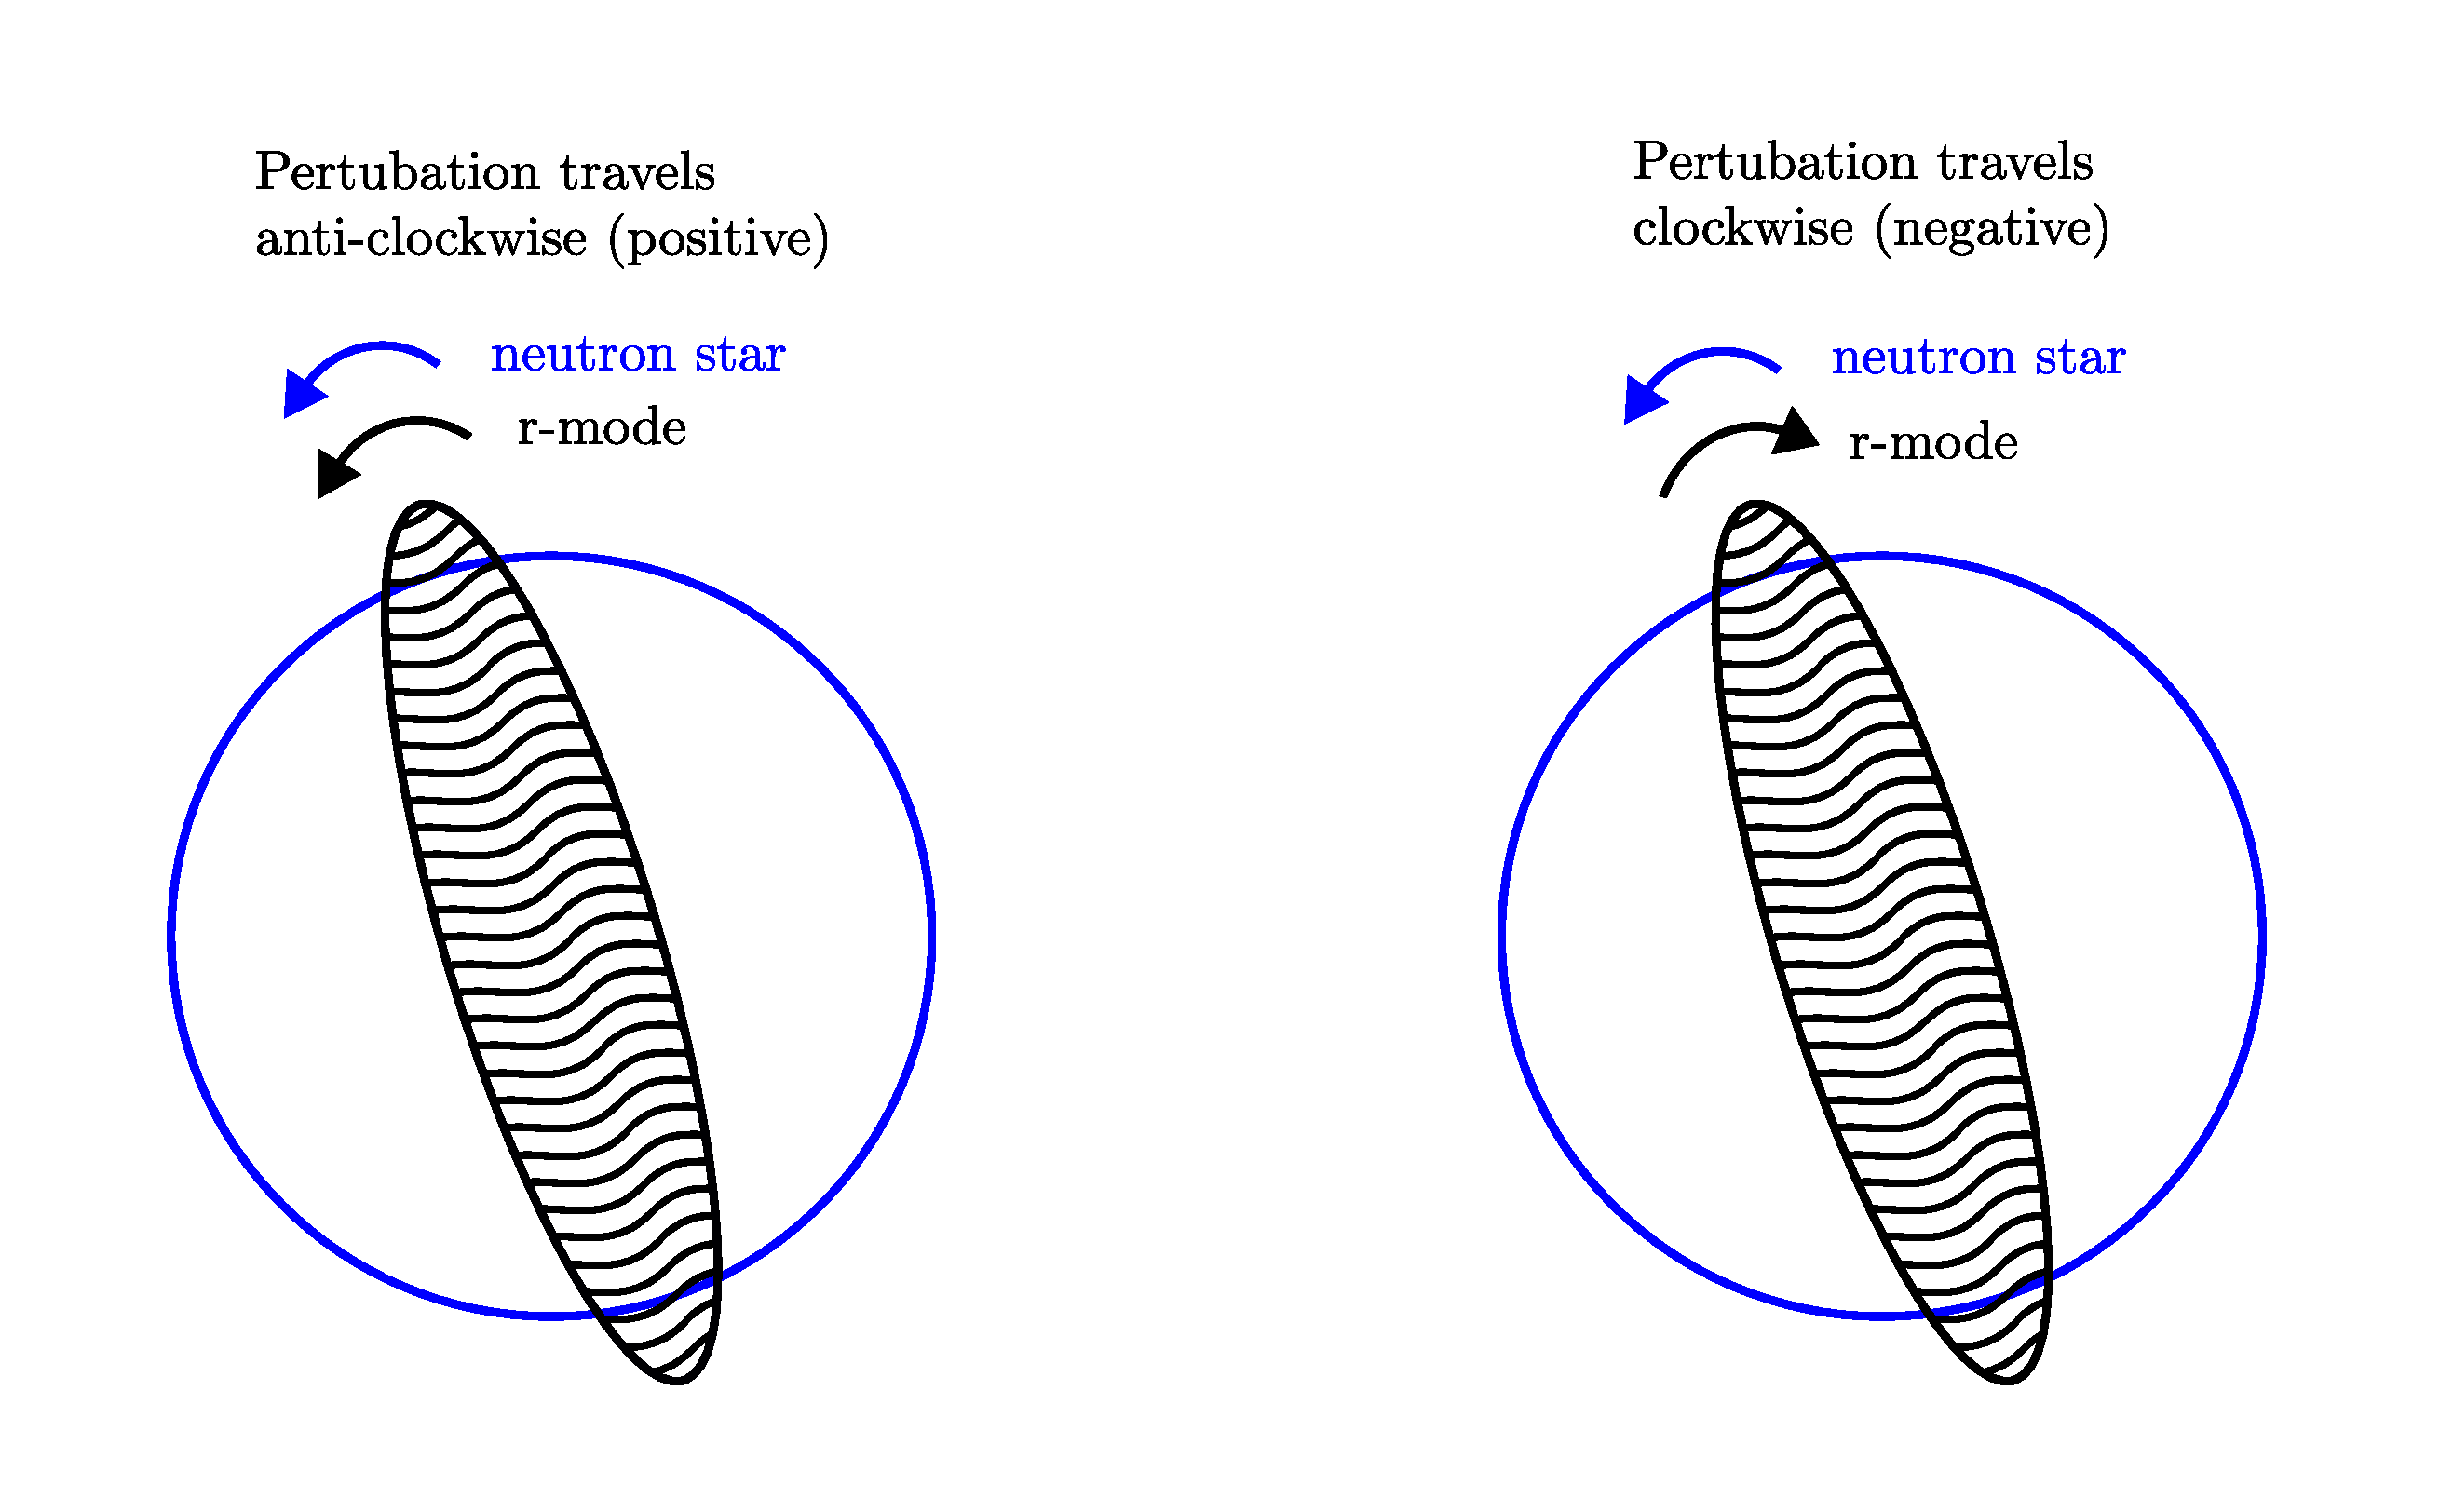
\includegraphics[width=\textwidth]{C1_intro/rmode.pdf}
	\caption[Generating \glspl{GW} from r-modes in neutron stars.]{The r-modes can travel in either direction in the star. in the case when the r-mode is moving clockwise and the neutron star is moving anti-clockwise, if the neutron star is rotating fast enough it can cause unstable emission of \gls{GW}. This image was reconstructed from \citep{jonesCFSInstability}.}
	\label{intro:source:cw:rmode}
\end{figure}
If these modes are excited in a non-rotating star, then they will emit \gls{GW} where the \gls{GW}  carries away angular momentum \citep{jonesCFSInstability}. 
For the mode travelling in a clockwise direction, this angular momentum is positive and the mode travelling anti-clockwise the angular momentum is negative. 
Therefore, the \gls{GW} is taking away either positive or negative angular momentum (adding angular momentum) depending on the direction of rotation.
The emission of \gls{GW} damps the modes and the magnitude of the perturbation decreases making them extremely difficult to detect.
Now if the neutron star is rotating, this can lead to an effect called the \gls{CFS} instability  \citep{chandrasekhar1970SolutionsTwo,friedman1978SecularInstability}. 
As the rotation speed of the neutron star increases, there are two different effects on the modes travelling in opposite directions. 
For the mode travelling anti-clockwise with the stars rotation, the mode will appear to be travelling faster, therefore, will emit more \gls{GW} taking away more angular momentum. This means that this mode will be damped more rapidly.
The interesting affect is for the mode travelling clockwise, opposite to the neutron stars rotation. 
At a certain rotation rate, the mode will be `frozen' from the observers perspective and no \gls{GW} will be emitted.
As the rotation rate increases further, the mode will appear to travel anti-clockwise to an observer, i.e. the mode is dragged in the opposite direction by the stars rotation. 
Here it is key to remember that this mode had negative angular momentum as in the neutron stars frame it is still travelling clockwise.
As the mode rotates its emits positive angular momentum, which is then subtracted from the modes negative angular momentum.
The magnitude of the angular momentum then increases such that more \glspl{GW} are released.
This effect causes the amplitude of the oscillation to grow and therefore become unstable.
Therefore, a neutron star is unstable to \gls{GW} emission if it is rotating sufficiently fast \citep{lasky2015GravitationalWaves}.
For a more detailed view on how r-modes generate \gls{GW} see \citep{owen1998GravitationalWaves,jonesCFSInstability}


%%%%%%%%%%%%%%%
%%%%%%%%%%%%%%
%%%%%%%%%%%%%%%
\section{\label{intro:detector}Detectors}
%%%%%%%%%%%%%%%%
%%%%%%%%%%%%%%
%%%%%%%%%%%%%%

The indirect detection of gravitational waves from the Hulse-Taylor binary pulsar system left little doubt that \gls{GW} existed. 
The real challenge was to design an instrument which could directly detect gravitational waves.
There were a number of different proposed methods for the design of the instrument, notably: resonant bar detectors, both ground based and space based interferometers, pulsar timing arrays and cosmic microwave background (CMB) detectors. 
The first resonant bar detector was designed and built by Joseph Weber \citep{weber1966ObservationThermal}. 
These are large cylinders of metal which should resonate as a gravitational wave passes by. 
There are a few different designs of this type of detector, including an omni-directional design \citep{dewaard2003MiniGRAILFirst}. 
Pulsar timing arrays aim to use the accurate arrival time of pulses from millisecond pulsars to measure \gls{GW} \citep{hobbs2017GravitationalWave}. As a \gls{GW} passes between the pulsar and the observer, the arrival time of the pulses should change by $\mathcal{O}(10)$ ns \citep{hobbs2017GravitationalWave}. 
Whilst a detection has not been made using pulsar timing arrays, these methods are still in use.
Cosmic microwave background detectors aimed to look for evidence of gravitational waves in the polarisation's of the CMB \citep{ade2018ConstraintsPrimordial}.  
These use the a range of detectors to look at the CMB however, are yet to confirm a detection of a \gls{GW} signal.
The most commonly known design of a \gls{GW} detector is the ground based interferometer, these made the first detection of \gls{GW} in 2015 \citep{abbott2016ObservationGravitational}. 
These are the focus of this section as the analysis that will follow uses data from the \gls{LIGO} detectors in the USA \citep{abbott2009LIGOLaser,aasi2015AdvancedLIGO} and Virgo detector in Italy \citep{acernese2015AdvancedVirgo,acernese2008StatusVirgo}. 

%%%%%%%%
%%%%%%%%%
\subsection{Laser Interferometers}
%%%%%%%%%%
%%%%%%%%%

Laser interferometers use the interference of light to measure a length with high precision.
The majority of this section will focus on ground based interferometers such as \gls{LIGO} and Virgo \citep{aasi2015AdvancedLIGO,acernese2015AdvancedVirgo}.
A simple design of an interferometer is shown in Fig.~\ref{detectors:interferometer:simple}. 
A laser beam is fired at a beam splitter which splits the light equally down two perpendicular arms. 
Each of these beams is reflected from a mirror at the end of either arm.
The light then returns to the beam splitter where the two beams are combined and sent to a photo-detector.
At the output, there is an interference pattern between the two beams.
If the length of one of the arms is changed then the interference pattern will change as the phase of one beam changes with respect to the other.
The phase difference of the light can be related to the wavelength of the light, $\lambda_l$ and the length of the detectors arms $L$ by
\begin{equation}
\label{intro:detectors:phasechange}
\Delta \phi \sim \frac{\Delta L}{\lambda_l},
\end{equation}
where $\Delta  \phi$ is the phase change and $\Delta L$ is the difference in the arm lengths.
An interferometer can then measure small changes in the mirrors position.
\begin{figure}[hp]
    \centering
    \begin{subfigure}[h]{0.6\linewidth}
    	 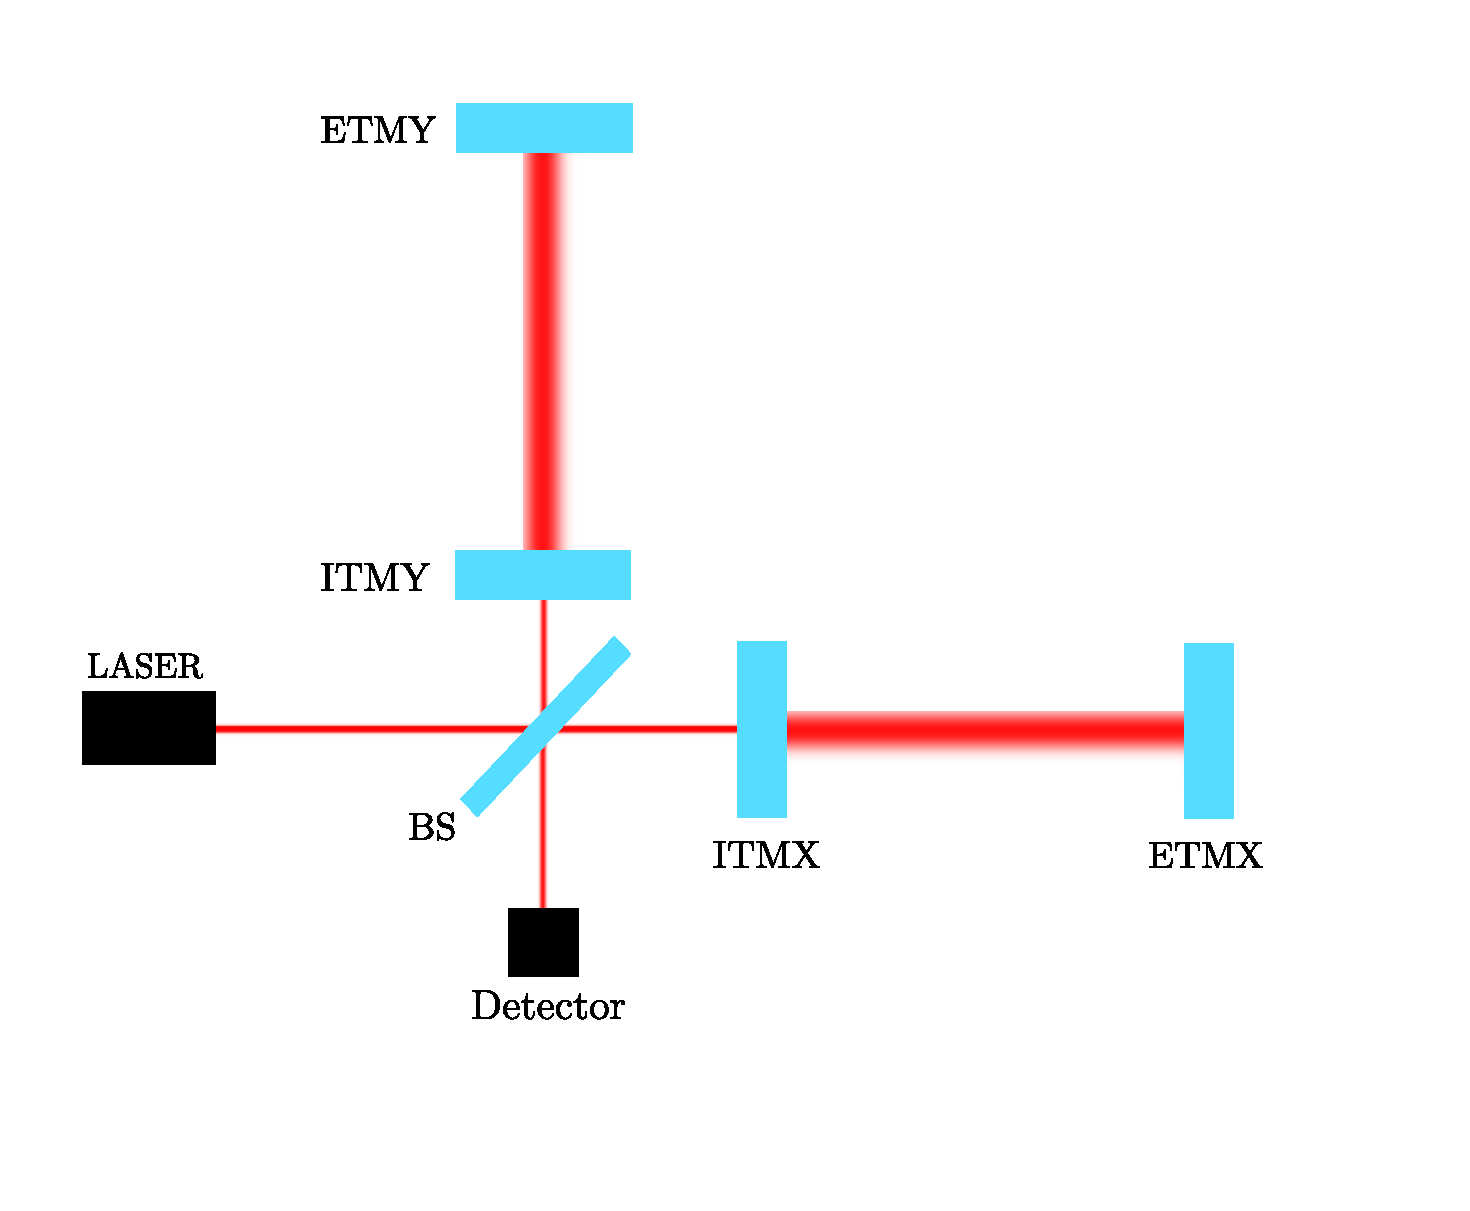
\includegraphics[width=\textwidth]{C1_intro/interferometer.pdf}
    	 \caption{Simple interferometer.}
    	 \label{detectors:interferometer:simple}
    \end{subfigure}
	\begin{subfigure}[h]{0.6\linewidth}
		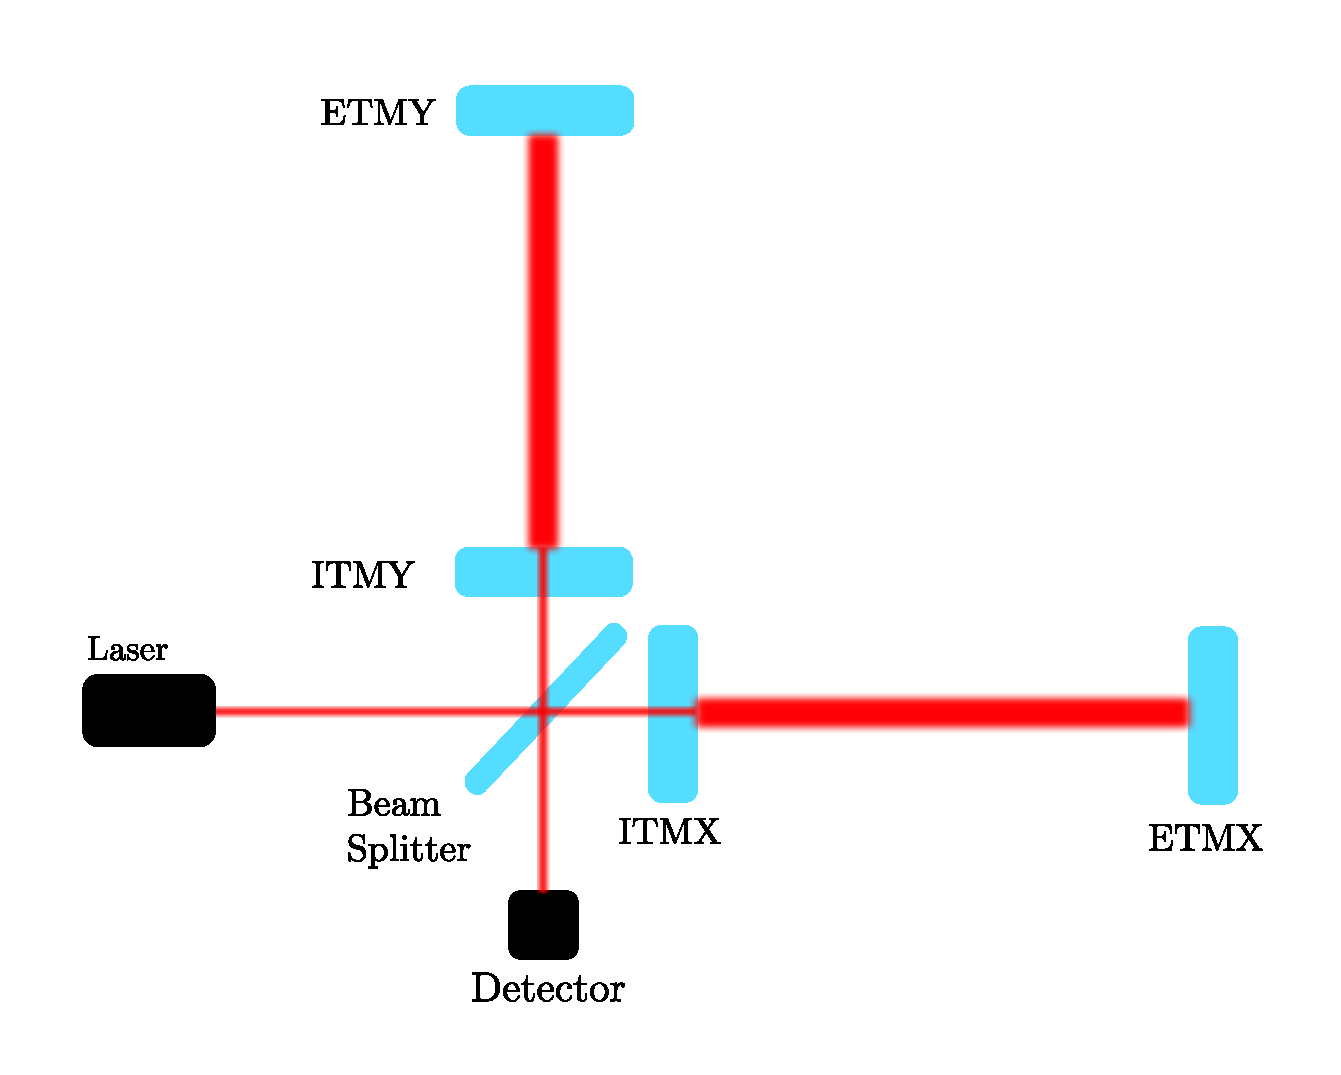
\includegraphics[width=\textwidth]{C1_intro/interferometer_fabry.pdf}
		\caption{Fabry-Perot interferometer.}
		\label{detectors:interferometer:fabry}
	\end{subfigure}
    \caption[Basic layout of the \gls{LIGO} detectors.]{\gls{LIGO} uses interferometry to make a detection. This has many additional features, one of which is shown above. ETMY and ETMX refer to the end test masses, which are just mirrors at the end of the interferometer arms. The beam splitter splits the Laser beam equally to each arm, this them recombines the beams back to the detector.
    ITMY and ITMX refer to the internal test masses, these create a Fabry-Perot cavity in the interferometers arms which can build up laser power. }
    \label{detectors:interferometer}
\end{figure}
%
This can be used in gravitational wave detection as the mirrors at the end of each arm of the interferometer can be treated as `free' test masses.
Figure \ref{gw:polarisations} shows the effect of a \gls{GW} on free test masses.
One can see this by looking at the proper separation between two test masses. 
If we place two test masses along the $x$ axis with separation $L_c$ where a gravitational wave is travelling along the $z$ axis, the proper distance between them is given by
\begin{equation}
    L = \int_{0}^{L_c} \sqrt{g_{xx}} dx,
\end{equation}
where $g_{xx} = 1 + h_{+}(t)$ is the combination of Eq.~\ref{intro:gravwave:metric} and Eq.~\ref{intro:gw:gravwave}. 
As the metric perturbation is small is can be can be expanded to first order, i.e. $\sqrt{g_{xx}} = \sqrt{1 + h_{+}(t)} \approx 1 + \frac{1}{2}h_{+}(t)$.
The proper distance is then
\begin{equation}
    \label{intro:detectors:properdist}
    \begin{split}
     L &\approx \int_{0}^{L_c} 1 + \frac{1}{2}h_{+}(t) dx \\
      &\approx L_c + L_c \frac{1}{2}h_{+}(t).
    \end{split}
\end{equation}
From Eq.~\ref{intro:detectors:properdist} on can see that in this configuration the plus polarisation of the gravitational wave causes the separation between the two test masses to oscillate \citep{flanagan2005BasicsGravitational}.
This can then be oscillation can be expressed as a fractional length change 
\begin{equation}
    \label{intro:detectors:fraclength}
    \frac{\delta L}{L} \approx \frac{1}{2} h_{+}.
\end{equation}
In the interferometer, this affect changes the lengths of the two arms which therefore changes $\Delta L$ in Eq.~\ref{intro:detectors:phasechange}.
The change of the interference pattern with time is then related to the \gls{GW}.
In practice the position of the two mirrors are held in position such that the interference pattern does not change.
The \gls{GW} is then related to the readout of the mirrors control system.

If one looks at Eq.~\ref{intro:detectors:fraclength} then if the mirrors at the end of the arms (ETMX and ETMY) are are placed further from the beam splitter, i.e. $L$ is increased, then the length change of the arms due to the gravitational wave will be greater.  
This means that increasing the length of the detectors arms increases the sensitivity of the interferometer. 
A method to achieve a similar affect without physically increasing the arm length is to use a Fabry-Perot cavity \citep{aasi2015AdvancedLIGO}, this is shown in Fig.~\ref{detectors:interferometer:fabry}.
This is where a semi-transparent mirror is placed between the beam splitter and end mirror in each arm (ITMX and ITMY).
Light enters this cavity and reflects back and forth between the two mirrors (ITMX and ETMX) a number of times before returning to the beam splitter.
This increases the time the light spends in one arm and is equivalent to increasing the arm length.
Actual ground based \gls{GW} detectors such as \gls{LIGO} \citep{abbott2009LIGOLaser} and Virgo \citep{acernese2015AdvancedVirgo} are much more complicated than described above.
They use many techniques to increase the sensitivity some of which are outlined in \citep{aasi2015AdvancedLIGO,abbott2009LIGOLaser}.
Many of these techniques are designed to reduce non-astrophysical affects on the detector, some of these effects and solutions are listed in Sec.~\ref{intro:detector:noise}.



%%%%%%%%%%%
%%%%%%%%%%
\subsubsection{Detector response}
%%%%%%%%%%
%%%%%%%%%

An important factor to know when using detector data to search for astrophysical signals is the detectors antenna pattern.
This measures how sensitive the detector is to different directions.
An example of the antenna response for \gls{LIGO} is in Fig.~\ref{intro:detectors:response} where the detectors arms lie on the x and y axis of the image.
This is clear when thinking about how a gravitational wave affects the test masses as in Fig.~\ref{gw:polarisations}. 
As the \gls{GW} is transverse to its propagation, when the detector is face on to the source, there will be a maximum change in the arm lengths and therefore a maximum sensitivity. 
In the same way the sensitivity will be at a minimum when edge to the source.

\begin{figure}
    \centering
    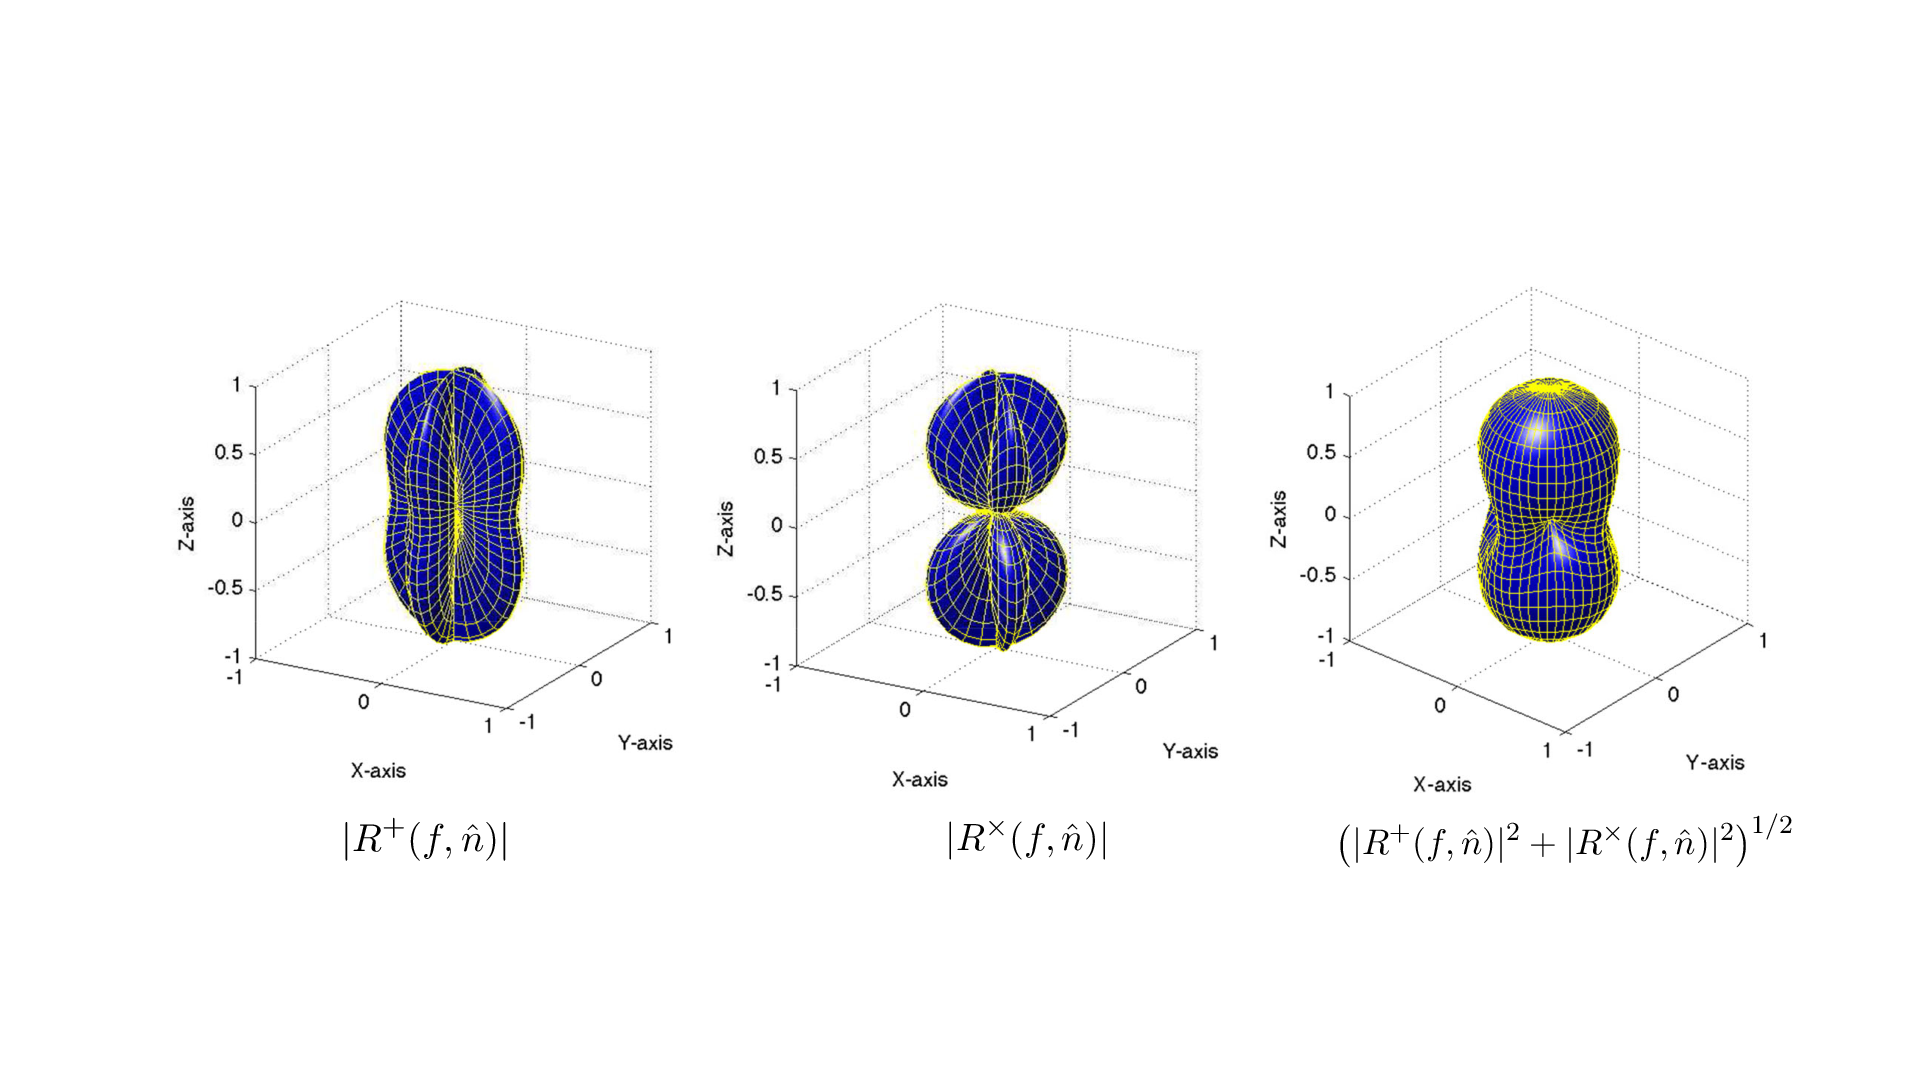
\includegraphics[width=\textwidth]{C1_intro/LIGO_beam_patterns.png}
    \caption[Antenna response of the \gls{LIGO} detectors.]{The antenna response is shown as in \citep{romano2019SearchesStochastic} for both the plus and cross polarisations and their average. The detectors arms lie on the x and y axis in the above plots. }
    \label{intro:detectors:response}
\end{figure}

%%%%%%%%%%%
%%%%%%%%%%
\subsubsection{\label{intro:detector:noise}Noise sources}
%%%%%%%%%%
%%%%%%%%%%

To increase the sensitivity of the \gls{LIGO} detectors, any effect on the output of the interferometer which is not astrophysical ideally needs to be reduced.
This involves understanding what causes certain noise features in the detector, and how the affect of these can be limited. 
Within the detector, there are many sources of noise.
Some of these noise sources and how they limit the detectors strain sensitivity are all shown in Fig.~\ref{detectors:noisesensitivity} from \citep{aasi2015AdvancedLIGO}.
\begin{figure}[h]
    \centering
    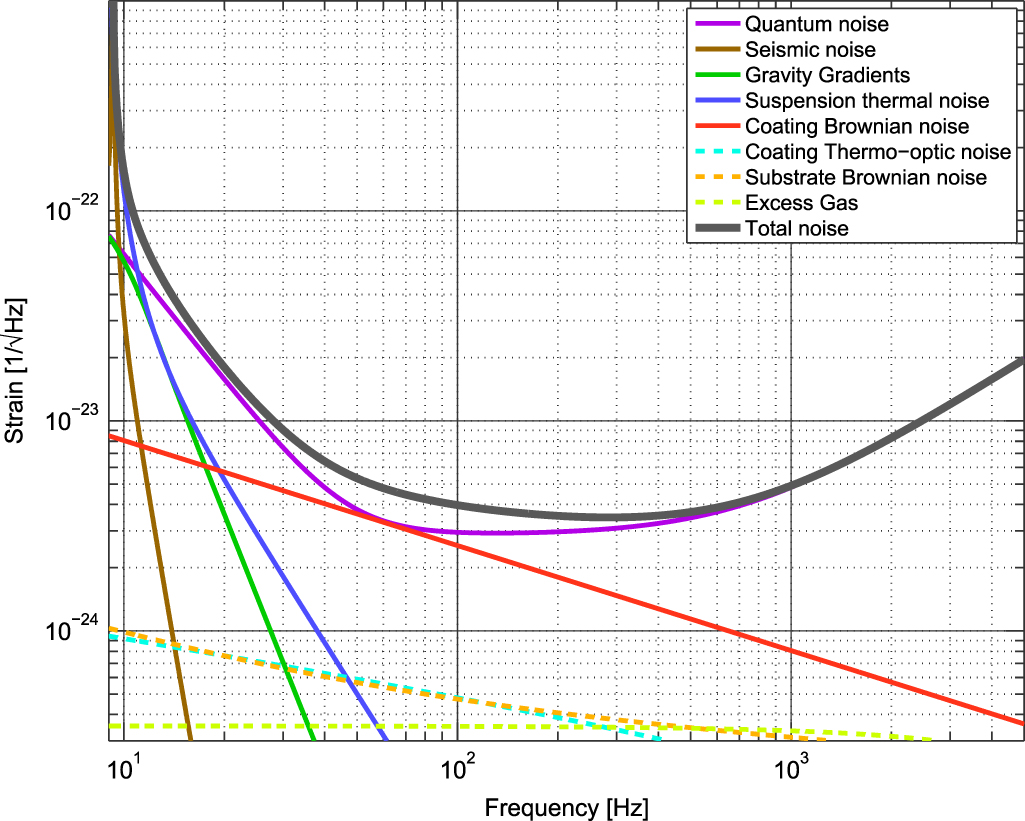
\includegraphics[width=0.9\textwidth]{C1_intro/noise_sensitivity.jpg}
    \caption[Example strain sensitivity curves for different noise sources in \gls{LIGO}.]{The different noise sources affect the sensitivity of the \gls{LIGO} detectors at different frequencies. This shows the various sources how the affect the noise curve \citep{aasi2015AdvancedLIGO}.}
    \label{detectors:noisesensitivity}
\end{figure}
Here I will summarise some of the limiting sources and also sources which become useful for understanding later sections.

\begin{description}
\item[Seismic noise] This originates from vibrations in the earth which can be from effects such as the earths seismic activity or anthropogenic sources. This affects lower lower frequencies of \glspl{LIGO} spectrum. This can be oscillations such as earthquakes or ocean waves. Seismic waves cause the mirrors to oscillate and induce a change in the length of the arm. This is reduced by having multi stage suspensions in the detectors which filter out the seismic oscillations \citep{matichard2015SeismicIsolation}.

\item[Coating noise] This is in general due to two main factors, the thermal noise of the coating and Brownian noise. The Brownian noise is from the mechanical dissipation in the coating and the thermal noise is due to thermal dissipation. The Brownian noise is the dominant factor as shown in Fig.~\ref{detectors:noisesensitivity}. These effects are limited by using different coatings on the mirrors \citep{abernathy0OverviewResearch}.

\item[Quantum noise] Quantum noise is a fundamental limit due to the statistical uncertainty of counting photons. This limits the sensitivity at many frequencies.There are methods to reduce this include squeezing of the light \citep{aasi2013EnhancedSensitivity}. 

\item[Electronics noise \joe{technical noise maybe}] Whilst this is not shown in Fig.~\ref{detectors:noisesensitivity}, this becomes important to searches described later. These have a different effect on the detector which is more narrowband frequency lines. This is generated by the digital and analogue electronics that are used to measure the signal. 
\end{description}

There are also many other sources of noise in the detector which I have not listed. However, these are often not the limiting cases of noise or are not relevant to this thesis.
In Sec.~\ref{detchar} I will go into more detail about specific noise sources in the detector known as instrumental lines and how they can be monitored and potentially removed. 













% and the other chapters

\chapter{\label{searchcw}Searching for continuous gravitational waves}
%%%%

%--------------------
% introduce problems in searching for CW
%---------------------
Continuous gravitational waves have particular challenges when it comes to their detection.
The nature of \gls{CW} are that they are long duration, this means that they would be observed for the entirety of a detectors observing runs. 
The signals also have an intrinsically small amplitude which is below the noise floor of current ground based detectors such as \gls{LIGO}.
This means the for a detection, the entire observing runs data will be needed to accumulate enough \gls{SNR} for a signal to be observed.
Given that \gls{LIGO} samples as $\sim 16$ kHz (generally downsampled to $\sim 4$ kHz) this leaves a huge amount of data which needs to be searched through.
As will be described in Sec.~\ref{searchcw:search:coherent} and \ref{searchcw:search:semi}, this requires a large amount of computational resources to perform these searches.
For some types of search, the parameter space can also be very large, this only adds to the computational time and in some cases makes it infeasible.

%---------------------
% Describe this chapter 
%--------------------------
Whilst I have described the potential sources of the signal and its approximate signal type in Sec.~\ref{intro:sources:cw},to perform a search the wave-form of a signal and how it is observed is needed.
In this section I will go into more detail on the `mountain' model in Sec.~\ref{intro:source:cw:mountain} and its wave-form description. 
This model is then used in various search methods for \gls{CW} signals.
In Sec.~\ref{searchcw:search} I will overview a subset of current searches for \gls{CW} signals.
Sec.~\ref{searchcw:motivation} explains the motivation for the majority of the work in this thesis.

%%%%%
%%%%%
\section{\label{searchcw:model}Continuous signal model}
%%%%
%%%%

The model of a \gls{GW} signal from a pulsar is relatively simple, it is a quasi-sinusoidal signal. This means that the signal is a sinusoid with a slowly varying frequency. One reason for the slow variance in the frequency is due to the energy loss to \gls{GW} as the pulsar spins down.
Here the signal is modelled to originate from an isolated triaxial neutron star rotating around a principal axis. 
The parameters of each pulsar can be split into two sections: the Doppler components ($\alpha,\delta,{\bm f}$) and its amplitude components ($\psi,\phi_0, \iota, h_0, \theta$). This ignores any orbital parameters which would be present if the star was in a binary systems and higher order frequency derivatives.
They are defined as follows: the sky positions $\alpha$ and $delta$ refer to the right ascension and declination. 
${\bm f}$ refers to the source frequency and its derivatives. 
$\psi$ and $\phi_0$ and $h_0 $ are the \gls{GW} polarisation, initial phase and amplitude respectively. 
$\iota$ is the inclination angle which is how much the source is tilted relative to the observer. 
$\theta$ is the `wobble angle' or the angle between the rotation axis and the symmetry axis of the neutron star.

The definition of the \gls{GW} from a neutron star here follows that in \citep{riles2017RecentSearches,schutz1998DataAnalysis,dupuis2005BayesianEstimation}. The amplitude of the \gls{GW} can be defined as,
\begin{equation}
\label{intro:cw:ht}
h(t) = F_+(t)h_{+}(t) +F_{\times}(t)h_{\times}(t),
\end{equation}
where $h_{+},h_{\times}$ are the plus and cross polarisations functions as in Eq.\ref{intro:gw:gravwave} and $F_{+},F_{\times}$ are the antenna pattern functions to the two polarisations.
These are defined by,
\begin{equation}
\label{intro:cw:amplitudes}
    \begin{split}
        h_{+}(t) &=  h_0 \frac{1 + \cos^2{(\iota)}}{2}\cos{\left(\Phi(t)\right)} \\
        h_{\times}(t) &= h_0  \cos{(\iota)} \sin{\left( \Phi(t)\right) } \\
    \end{split}
\end{equation}
The plus and cross polarised components then depend on the \gls{GW} amplitude $h_0$, the inclination angle of the source $\iota$ and the phase evolution of the \gls{GW}. Here I have chosen to assume a small wobble angle $\theta$, however, this is included in \citep{schutz1998DataAnalysis}. The phase of the wave $\Phi(t_{{\rm SSB}})$ at the \gls{SSB} can be defined as,
\begin{equation}
\label{searchcw:model:phase}
    \Phi(t_{{\rm SSB}}) = \phi_0 + 2\pi\left[ f(t_{{\rm SSB}} - t_0) + \frac{1}{2} \dot{f} (t_{{\rm SSB}} - t_0)^2 + .....\right] .
\end{equation}
This consists of an initial phase $\phi_0$ which is the phase at time $t_0$, the frequency of the signal $f$ and its derivative ${\dot{f}}$ at time $t_0$. Here we show the phase to second order, however, this can be easily extended if necessary. 
The time at the \gls{SSB} $t_{{\rm SSB}}$ can be transformed to the time $t$ at the detector by,
\begin{equation}
t_{{\rm SSB}} = t - \frac{\mathbf{r}_d \cdot \mathbf{k}}{c} + \delta_t.
\end{equation}
Here $\mathbf{r}_d$ is the position of the detector with reference to the \gls{SSB}, $\mathbf{k}$ is a unit vector in the direction of the source. This essentially takes into account the Doppler shift of the signal due to the movement of the detector, i.e. as the earth rotates and orbits the sun. $c$ is the speed of light and $\delta t$ is extra corrections from the Einstein, Binary and Shapiro delay \citep{}.
The amplitudes $h_0$ in Eq.~\ref{intro:cw:amplitudes} are defined by,
\begin{equation}
    h_0 = \frac{16 \pi^2 G}{c^4} \frac{\epsilon I f^2}{r},
\end{equation}
where $G$ is the gravitational constant, $c$ is the speed of light, $\epsilon$ is the ellipticity of the star, $f$ is the sum of the frequency of rotation of the star and the frequency of precession, $r$ is the distance to the star and $I_{zz}$ is the moment of inertia with respect to the rotation axis $z$.
The ellipticity of the star $\epsilon$ is a measure of the distortion of the star around its rotation axis and is defined by,
\begin{equation}
    \epsilon = \frac{I_{xx} - I_{yy}}{I_{zz}},
\end{equation}
where $I_{xx}, I_{yy}$ and $I_{zz}$ are the moments of inertia for each axis.

In Eq.~\ref{intro:cw:ht}, $F_+(t)$ and $F_{\times}(t)$ are the antenna pattern functions of the detector. 
These describe how sensitive a detector is to a particular location on the sky at any given time. 
The amplitude of the signal will vary dependent on the orientation and location of the detector relative to the source.
This is described in Sec.~\ref{intro:detector} and the response to sky location is shown in Fig.~\ref{intro:detectors:response}.
These components are defined in \citep{schutz1998DataAnalysis} as,
\begin{equation}
\label{intro:cw:antenna}
\begin{split}
F_{+}(t) &= \sin{\zeta}[a(t)\cos{(2\psi)} + b(t)\sin{(2\psi)}], \\
F_{\times}(t) &= \sin{\zeta}[b(t) \cos{(2\psi)} - a(t)\sin{(2\psi)}],
\end{split}
\end{equation}
where $\zeta$ is the angle between the arms of the detectors, $\psi$ is the polarisation angle of the \gls{GW} and $a(t)$ and $b(t)$ are defined in \citep{schutz1998DataAnalysis} and relate the sky location to the orientation of the detector at a given time. 
A full derivation of this can be found in \citep{schutz1998DataAnalysis} where each of these terms are expanded.

Eqs.~\ref{intro:cw:ht} - \ref{intro:cw:antenna} then describe the amplitude and phase evolution of a signal at a given detector location and orientation.



%%%%%%%%%%%%%
%%%%%%%%%%%%%%%
%%%%%%%%%%%%%%%%
\section{\label{intro:prob} Bayes Theorem}
%%%%%%%%%%%%%%%
%%%%%%%%%%%%%%%%
%%%%%%%%%%%%%%%%%

A key part in understanding the different methods to search for \gls{GW} or any data analysis, is understanding probability and statistics. 
This gives understanding of the random processes underlying all measured quantities. 
Whilst there are generally two approaches to statistics: Frequentist and Bayesian, here I will focus on the Bayesian approach.  

%%%%%%%%%%%%%
%%%%%%%%%%%%%
\subsection{\label{intro:prob:basic}Basic probability}
%%%%%%%%%%%%%%
%%%%%%%%%%%%%%

Initially I will define some basic concepts of probability.
We can define the probability of some event $A$ as $p(A)$ where probabilities follow $0 \leq p(A) \leq 1$ and some other event $B$ which has a probability $p(B)$ and follows $0 \leq p(B) \leq 1$.

\begin{description}
	\item [Union]
	A union is the probability of either and event $A$ happening or event $B$ happening. This is written as, $p(A \cup B)$.
	
	\item [Intersection]
	An intersection is then the probability that both and event $A$ and an event $B$ happens. This is written as $p(A \cap B)$.
	
	\item [Independent and dependent Events]
	If the events $A$ and $B$ are independent, i.e. the event $A$ does not affect the outcome of event $B$, then,
	\begin{equation}
	p(A \cap B) = p(A)p(B).
	\end{equation}
	However, if the event $A$ is dependent on event $B$, i.e. the event $A$ affects event $B$ or vice versa, then the joint probability of both events is,
	\begin{equation}
	\label{dependentevent}
	p(A \cap B) = p(A)p(B \mid A) = p(B)p(A \mid B).
	\end{equation}
	Here $p(B \mid A)$ means the probability of event $B$ happening given that event $A$ has happened.
	
	\item [Conditional probability]
	Conditional probability arises from situations where the outcome of one event will affect the outcome of future events.
	The definition of this arises from the the dependent events defined above in Eq.~\ref{dependentevent},
	\begin{equation}
	p(A \mid B) = \frac{p(A \cap B)}{p(B)}.
	\end{equation}
	
	\item [Bayes Theorem]
	Bayes theorem can then be defined using conditional probabilities. i.e we can use
	\begin{equation}
	p(A \mid B) = \frac{p(A \cap B)}{p(B)} \quad \rm{and} \quad p(B \mid A) = \frac{p(A \cap B)}{p(A)}
	\end{equation}
	such that then,
	\begin{equation}
	p(B)p(A \mid B) = p(A)p(B \mid A)
	\end{equation}
	and this is rearranged to Bayes theorem,
	\begin{equation}
	p(A \mid B) = \frac{p(A)p(B \mid A)}{p(B)}
	\end{equation}
	
\end{description}

%%%%%%%%%%%%%%%%%
%%%%%%%%%%%%%%%%%%
\subsection{\label{intro:prob:bayes}Bayesian Inference}
%%%%%%%%%%%%%%%%%%%
%%%%%%%%%%%%%%%

We can take Bayes theorem from Sec.~\ref{intro:prob:basic} and apply it to a problem which involves infering some parameters from some model. Here we can relabel the events $A$ and $B$ with the data ${\bm d}$ and the parameters ${\bm \theta}$ of some model $I$.
Eq.~\ref{intro:prob:bayes} then becomes,
\begin{equation}
\label{intro:bayes:bayes}
p({\bm \theta} \mid {\bm d}, I) = \frac{p({\bm \theta}, I)p({\bm d} \mid {\bm \theta}, I)}{p({\bm d} \mid I)}
\end{equation}
where each of the components are assigned names: $p({\bm \theta} \mid {\bm d})$ is the posterior distribution, $p({\bm \theta})$ is the prior distribution,  $p({\bm d} \mid {\bm \theta})$ is the likelihood and $p({\bm d})$ is the evidence.

\begin{description}
	\item [Posterior]
	The posterior distribution describes the probability of a parameter ${\bf \theta}$ in some model $I$ given some data $d$. For many problems this is the distribution which is most useful as it informs you the most likely set of parameters of you model given some observation.
	\item [Prior]
	The Prior distribution is a key part of Bayesian statistics. This distribution describes any information which you have prior to the observation. This is a distribution defined by the user, where you define a distribution of the parameters based on what you expect to be true.
	\item [Likelihood]
	The likelihood is where the observation is included in the calculation. This tells you how probable it is to get the observed data $d$ given the model $I$ with the set of parameters $\theta$. 
	\item [Evidence]
	The evidence is the probability of the data itself given the choice of model. This is found by integrating the likelihood over all possible values of ${\bm \theta}$ weighting them by our prior belief of that value of ${\bm \theta}$. This known as a marginal distribution and is defined by,
	\begin{equation}
	\label{intro:bayes:evidence}
	p({\bm d} \mid I) = \int p({\bm \theta}, I)p({\bm d} \mid {\bm \theta}, I) d{\bm \theta}.
	\end{equation}
\end{description}


Bayes theorem then gives a description of the probability distribution of some parameters in a model given some observation.
Often when using Bayesian statistics the aim is to find posterior distribution of parameters.
There are very few cases where this can be calculated analytically, therefore, numerical methods are almost always used to find the posterior.
This can be difficult to calculate numerically especially in problems where the parameters space has many dimensions.
The most difficult part to calculate is the evidence in Eq.~\ref{intro:bayes:evidence}, this involves calculating an integral over all possible parameters.
There is however, a way around having to calculate this. For any given mode $I$, the evidence $p({\bm d}\mid I)$ is the same for any set of parameters ${\bm \theta}$ in Eq.~\ref{intro:bayes:bayes}. 
The evidence is then just a normalisation factor for the posterior distribution. 
When different models are not being compared, and we assume the model $I$ to be true, we no longer need to calculate the evidence.
The posterior distribution can then be found by sampling,
\begin{equation}
p({\bm \theta} \mid {\bm d}, I) \propto p({\bm \theta}, I)p({\bm d} \mid {\bm \theta}, I).
\end{equation}
To find this posterior you could then calculate (sample) the value for every point in parameter space. This however, is very computationally expensive and often the posterior distribution is located in a small area in parameter space. 
Therefore, the majority of the time is sampling a area of parameter space where the posterior is close to zero, and this is not particularly useful. 
A method titled \gls{MCMC} was proposed \citep{metropolis1953EquationState} to deal with this issue, more information on this can be found in \citep{vanravenzwaaij2018SimpleIntroduction,sharma2017MarkovChain}.
This builds up the posterior distribution by randomly jumping around in the parameter space.
It starts by calculating the posterior value for a particular point in parameter space. Then it will randomly jump to another parameter space point. 
The posterior can then be calculated again, if the posterior value is higher then the jump is `accepted'. This just means that the parameter values of this point are stored.
If the posterior value is lower than the previous step then the jump is accepted with some probability. This means that there is a random chance that a value lower than the current is accepted.
As the accepted positions aim for areas where the posterior is higher, \gls{MCMC} does not waste time calculating areas in parameter space of low posterior values.
The samples which were accepted then build the posterior distribution. 

In certain situations it can be useful to calculate the evidence in Eq.\ref{intro:bayes:evidence}. 
For example, if there are two different models which could represent the data, the evidence can be used to determine which of the two models is more likely.
This is known as a Bayes factor where two models $I_1$ and $I_2$ are compares and is defined as,
\begin{equation}
B = \frac{p({\bm d} \mid I_1)}{p({\bm d} \mid I_2)}
\end{equation}
This then requires the calculation of the evidence.
To estimate the evidence efficiently a method known as Nested sampling can be used, this is explained in detail in \citep{skilling2006NestedSampling,speagle2019DynestyDynamic}.
By calculating the Bayes factor, which is similar to a likelihood ratio, one can find the posterior odds of a particular model by using,
\begin{equation}
\frac{p(I_1 \mid \mathbf{d})}{p(I_2 \mid \mathbf{d})} = \frac{p(I_1)}{p(I_2)} \frac{p(\mathbf{d} \mid I_1)}{p(\mathbf{d} \mid I_2)}.
\end{equation}
The can be written as \textit{posterior odds = prior odds $\times$ bayes factor}. This is then a comparison of how likely different models are given some observation. 

The methods described above then provide a way to estimate parameters of a model given some data. 
Also this provides a way to compare different models given some observation.
In following sections the methods described above are used to estimate various parameters.


%%%%%%%%%%%55
%%%%%%%%%%%%%
\section{\label{searchcw:search} Continuous wave searches}
%%%%%%%%%%%%%%%%%%
%%%%%%%%%%%%%%%%%%

There are many different methods to search for continuous gravitational waves.
They can be split into three general categories: Targeted searches, Directed searches and All-sky searches.
The main difference between these different categories is the amount which is known about the source prior to the search.
For targeted searches the sky position $(\alpha,\delta)$ and rotation frequency are known from electromagnetic observations, i.e. X-ray, radio or $\gamma$-ray.
Directed searches have information on the sky position $(\alpha,\delta)$ but not the rotation frequency.
For all-sky searches, there is no prior knowledge of the pulsar, therefore, is a search for unknown pulsars.
In general the searches in each of these categories use two distinct techniques: Fully coherent searches and Semi-coherent searches

%%%%%%
%%%%%%
\subsection{\label{searchcw:search:coherent}Fully coherent}
%%%%%%
%%%%%%

A Fully coherent search generally uses a pre generated waveform which follows the model described in Sec.~\ref{searchcw:model}. 
This contains all the phase information of the signal.
The set of parameters which generated the waveform which `matches' the best can then be considered as the optimum set of parameters given the data.
This is known as a matched filter \citep{} and is used in \gls{CW} searches in \citep{dupuis2005BayesianEstimation,}.

The matched filter maximises the signal to noise ratio for a given filter, in this case the filter is our \gls{CW} model. 
The matched filter used for \gls{CW} models is defined in \citep{prix2007SearchContinuous} and it titled the $\mathcal{F}$-statistic. 
This essentially maximises a likelihood with respect to the parameters.
If one assumes that the noise $n$ is Gaussian and zero mean, the data $x$ can be written as,
\begin{equation}
		x(t) = n(t) + h(t).
\end{equation}
The likelihood can then be written as,
\begin{equation}
		\log \Lambda = \left( x \mid h \right) - \frac{1}{2} \left( h \mid h\right) 
\end{equation}
where the product $(x \mid y)$ is defined as,
\begin{equation}
		\left( x \mid y \right) = 4 \mathcal{R} \int^{\infty}_{-\infty}  \frac{\tilde{x}^{{\rm X}}(f) \tilde{y}^{{\rm X *}}(f)  }{S^{X}(f)} \mathrm{d}f.
\end{equation}
This is fulle expanded into the $\mathcal{F}$-statistic in \citep{schutz1998DataAnalysis}, however, it is essentially this likelihood function which is maximised. 


Targeted searches look for a specific pulsar which has been observed in the electromagnetic spectrum.
These observations give information such as the sky position and the frequency evolution of the source.
Using knowledge of the earths position around the sun, which is well known, one can use the accurate sky position and frequency of a known source to find its phase evolution in Eq.~\ref{searchcw:model:phase}.
This mean that for this type of search one can maximise the likelihood with respect to the parameters  $h_0, \phi_0, \iota$ and $\psi$.
Another method which uses templates is described in \citep{dupuis2005BayesianEstimation}, this uses a Bayesian approach.

This type of search can take long periods of time. 
This is due both to the size of the parameter space and the amount of data which needs to be searched.
\gls{CW} searches need long observation times in order to accumulate the required \gls{SNR} for detection.
Therefore, most searches use data from an entire \gls{LIGO} observing run which can last for $\mathcal{O}(1)$ years.
Given that the sampling rate for the \gls{GW} channel is $16$ kHz usually downsampled to $\sim 4$ kHz, the quantity of data is large. 


Whilst the fully coherent matched filter searches have methods to reduce the computational time for known sources, in all-sky and directed searches, this type of search is no feasible. 
This is because all-sky and directed searches have a wider parameter space, therefore, enough templates need to be made to sufficiently cover the large parameter space. 
This task quickly becomes impossible for coherent matched filtering for an entire observing run due to the amount of time needed. This problem led to the development of semi-coherent searches which will be introduced in the next section. 


%%%%%%
%%%%%%
\subsection{\label{searchcw:search:semi}Semi coherent}
%%%%%%
%%%%%%

Semi-coherent searches offered a solution to searching over large parameters spaces and large amounts of data. 
As is directed and all-sky searches the phase evolution of the source is not known, one cannot use a coherent search for the entire observing run.
It may however, be possible to approximately describe the phase for a shorter length of time known as the coherence time, $T_{coh}$.
The general idea of a semi-coherent search is to break the data-set into smaller section which each can be analysed coherently.
The coherent analysis can use the matched filter as described in Sec.~\ref{searchcw:search:coherent} or another method such as a Fourier transform.
The results from each of these individual sections can the be combined incoherently using various methods which will be summarised later. 
This method can greatly reduce the time taken for the analysis depending on the coherence length, however, will always come with some loss in sensitivity. 

There are many different types of semi-coherent search which use various methods to incoherently combine the coherently analysed results. 
I will summarise some of these searches below, some of these searches were summarised and compared in \citep{walsh2016ComparisonMethods}.
Many of these searches use a set of 1800s long Fourier transforms as the input data, known as \glspl{SFT}. This is a default for many all-sky \gls{CW} searches, where it assumes that the signal remains within one frequency bin during that 1800s.

\begin{description}
	
	\item[Stack-slide] Stack uses a set of Fourier transforms of the data known as \glspl{SFT}, specifically it uses the power spectrum of these. Each of the separate Fourier transforms (segments) is shifted up or down relative to the others to account for the Doppler modulation of the source. The power from each can then be stacked. More explanation of this can be found in \citep{brady2000SearchingPeriodic, cutler2005ImprovedStackslide}  
	
	\item[Hough] The Hough transform is based on the stack-slide algorithm. The main difference is that the detection statistic for each segment is assigned a weight of 0 or 1 depending if it crossed a detection threshold. The Hough transform can the create a `Hough map' which gives a view of the data in parameter space. This approach is explained in greater detail in \citep{krishnan2004HoughTransform,antonucci2008DetectionPeriodic}. 
	This method has been applied in two main ways known as Sky Hough \citep{krishnan2004HoughTransform}and Frequency Hough \citep{antonucci2008DetectionPeriodic,astone2014MethodAllsky}.
	
	\item[Einstein@Home] Einstein at home uses the $\mathcal{F}$-statistic mentioned above in various stages. It has a hierarchical structure where it starts with a coarse parameter space with shorter coherence times. This search then provides a list of candidates from this run in coarse parameter space. The parameter space is then more finely sampled around the parameters of the candidates and this process is repeated. The search can also increases the coherence length when searching around given candidates to improve the sensitivity of the search. This algorithm has many additions which are explained in more detail in \citep{singh2016ResultsAllsky,papa2016HierarchicalFollowup,walsh2016ComparisonMethods}
	This provides the most sensitive all-sky \gls{CW} search, however, uses a large amount of computing power. This is achieved by using a distributed computing projects, more details can be found at \citep{EinsteinHome}. 
	
	\item[Time domain $\mathcal{F}$-statistic] The time domain $\mathcal{F}$-statistic splits the data into narrowband segments of length $\sim$ 2 days \citep{walsh2016ComparisonMethods}. Then a coherent search using the $\mathcal{F}$-statistic is applied to each of these segments. Values of this statistic above a threshold are stored. Coincidences are then found in each segment, where candidates are selected best on a given threshold. This is explained in greater detail in \citep{aasi2014ImplementationTextdollar,walsh2016ComparisonMethods}.
	
	
	\item[Powerflux] Powerflux uses a standard set of 1800s \glspl{SFT}. For each point in parameter space, the power in this set of \glspl{SFT} along the frequency track is recorded. This power is then weighted depending on the antenna pattern and noise of the detector. In longer stretches of $\sim$ 1 month, the weighted power is summed. Any point in parameter space which produces high power in each of these stretches is identified as a potential signal. This search can then be repeated around each candidate with a finer resolution in parameter space. This is explained in more detail and tested in \citep{abadie2012AllskySearch,walsh2016ComparisonMethods,ligoscientificcollaborationandvirgocollaboration2016ComprehensiveAllsky}
	
	\item[Viterbi] The Viterbi algorithm \citep{viterbi1967ErrorBounds} has been used in \citep{sun2018HiddenMarkov, suvorova2017HiddenMarkov,abbott2017SearchGravitational, abbott2018SearchGravitational, sun2018ApplicationHidden} to search for a \glspl{CW} with randomly wandering spin frequency. This algorithm was applied to specific sources, where the $\mathcal{F}$-statistic is used on short duration segments which are then incoherently combined using the Viterbi algorithm.
	
	
\end{description}


Each of these searches uses a large computational cost. In \citep{walsh2016ComparisonMethods} a \gls{MDC} was conducted to compare the sensitivity of some of the searches, where an expected runtime for and O1 search was presented. Result in O1 for some of these searches can now be found in \citep{ligoscientificcollaborationandvirgocollaboration2017AllskySearch}.
The results of this are shown in Tab.\ref{searchcw:search:semi:cost}.
\begin{table}
	\centering
	%
	\caption{From \citep{walsh2016ComparisonMethods}, shows the computational cost for the first 4 months of advanced \gls{LIGO} for each search. One \gls{MSU}, where one standard unit is one core-hour on a standard core. ` Expected computational costs of searches using the first four months of advanced \gls{LIGO} data with each search pipeline. These estimates are for a different data observing time from that of the \gls{MDC}, and do not cover the same parameter space as each other or the \gls{MDC}. The Einstein@Home searches uses the computing resources of the Einstein@Home project and is designed to run for 6 - 10 months in the Einstein@Home grid.'  \label{searchcw:search:semi:cost}}
	
	%
	\bgroup
	\def\arraystretch{1.5}
	\centering
	\begin{tabular}{|c c|}
		\hline
		Pipeline & Expected runtume of O1 search \\
		\hline
		Powerflux & 6.8 MSU \\

		Time domain $\mathcal{F}$-statistic & 1.6 MSU\\

		Frequency Hough & 0.9 MSU \\

		Sky Hough & 0.9 MSU\\
		\hline
		Einstein@Home & 100-170 MSU\\
		\hline

	\end{tabular}
	\egroup
\end{table}
Even the fastest of these searches takes close to 1 million core-hours to search through four months of data.
This is one of the larger current issued in \gls{CW} searches as this is a slow process and running computing clusters can be costly.


%%%%%%%%%5
%%%%%%%%%%%
\section{\label{searchcw:motivation}Motivation}
%%%%%%%%%%
%%%%%%%%%%

The searches described in Sec.~\ref{searchcw:search} are computationally expensive, where the fastest takes $\sim$1 million core-hours to search through 4 months of O1 data.
Many of these searches use well-modelled signals to compare to the data. This leads to the parameter space having to be finely sampled such that it is sufficiently covered.  
The motivation for much of the work then follows from these points. 
The aim was to develop searches which used minimal computational resources and could work outside of the \gls{CW} model in Sec.~\ref{searchcw:model}.
This thesis then outlines algorithms which can reduce this computational time of searches for \gls{CW} whilst retaining as much sensitivity to \gls{CW} signals as possible.
There are two main sections which follow, Sec.~\ref{soap} will outline an essentially un-modelled \gls{CW} search method which uses the Viterbi algorithm.
Sec~\ref{machine} will then outline an method which used machine learning, specifically \glspl{CNN} as both its own \gls{CW} search and an extension to the search described in Sec.~\ref{soap}.
Following chapters then explain applications of these searches.




\chapter{\label{soap} SOAP: A generalised application of the Viterbi algorithm to searches for continuous gravitational-wave signals.}

The SOAP search is a semi-coherent \gls{CW} search algorithm that aims to
reduce the computational time needed to find a potential signal.  The algorithm
looks though narrow-banded time-frequency spectrograms of data to find the
`most probable track' in frequency through it.  This `most probable track' is
then the most likely track which a pulsars frequency would follow.  The
motivation of the search is simple, if we looked at a frequency band in a
spectrogram as in Fig.~\ref{soap:motivation:plot}, we could find every possible
randomly wandering track from a starting frequency bin to an end frequency bin.
For each of these tracks the sum of the spectrogram power along the track can
be found such that for each track there is a single value.
Fig.~\ref{soap:motivation:plot} shows a histogram of a subset of these values.
If there is a signal present in this band then it could be assumed that the
signal which gives the highest sum of spectrogram power is the track which is
most likely to follow the signals frequency track~\chris{It's not clear why you
can assume this. The point is that the we would expect the maximum track in
noise to have certain properties including it's likely summed value. We can
only distinguish things from that distribution if they show properties
different to the noise distribution. A loud enough signal will do that.}.  In
Fig.~\ref{soap:motivation:plot} the optimum track in red shows
gives~\chris{typo} a
statistic value of $\sim 1700$ which is far outside the main distribution of
summed powers.  The red track follows that~\chris{typo} an injected signal.  This
demonstrates that the sum of the spectrogram power along a track which follows
a signal is outside the distribution of tracks randomly walk~\chris{typo} through noise.
Therefore, it can be assumed that if the frequency track with the highest sum
of spectrogram power is found, then the corresponding track is most likely
for~\chris{typo}
follow a signal.  Now as calculating all possible tracks is computationally
expensive~\chris{not a sentence}. Given that in the example in Fig.~\ref{soap:motivation:plot}, the
spectrogram is~\chris{typo} frequency 180 bins wide $M$ and 400 time segments
long $N$~\chris{grammar} and
after each segment the track has $T$ possible options to jump to (in this case
it is 180 options), The total number of possible tracks is $T^{M \times N}$.
For this spectrogram this value is $180^{72000}$~\chris{whatever number this is
you should cast it in powers of 10}, this is an unreasonable
number of tracks to possibly calculate~\chris{I also think it's wrong. If at
each step you have 180 possible jumps then starting at a single bin you have
$T^N$ possible paths. Counting all possible starting bins you have $MT^N$.}. This is where the Viterbi algorithm
\citep{viterbi1967ErrorBounds} is useful as it can efficiently find the track
which gives the maximum sum of power. For an equivalent search the Viterbi
algorithm would have to do $T*M*N$~\chris{droip the * notation} calculations for find the optimum track. The
method of how this is~\chris{grammar} done is explained in the following
sections.

The majority of this chapter that follows has been reviewed and published as in
\citep{bayley2019GeneralizedApplication}. This was work done by the author
under the supervision of Prof. Graham Woan and Dr. Chris Messenger.  The
exceptions are work in Sec.~\ref{soap:lineawareamp},
Sec.~\ref{soap:las:optimisation}, Sec.~\ref{soap:sensfreq} and
Sec.~\ref{soap:sens:other} which is supplementary material~\chris{were
the specific sections mentioned not done under out supervision? Also, 3.11.3
and 3.11.4 are within 3.11 so which exact sections are new? It's not clear.}.


\begin{figure}

\centering
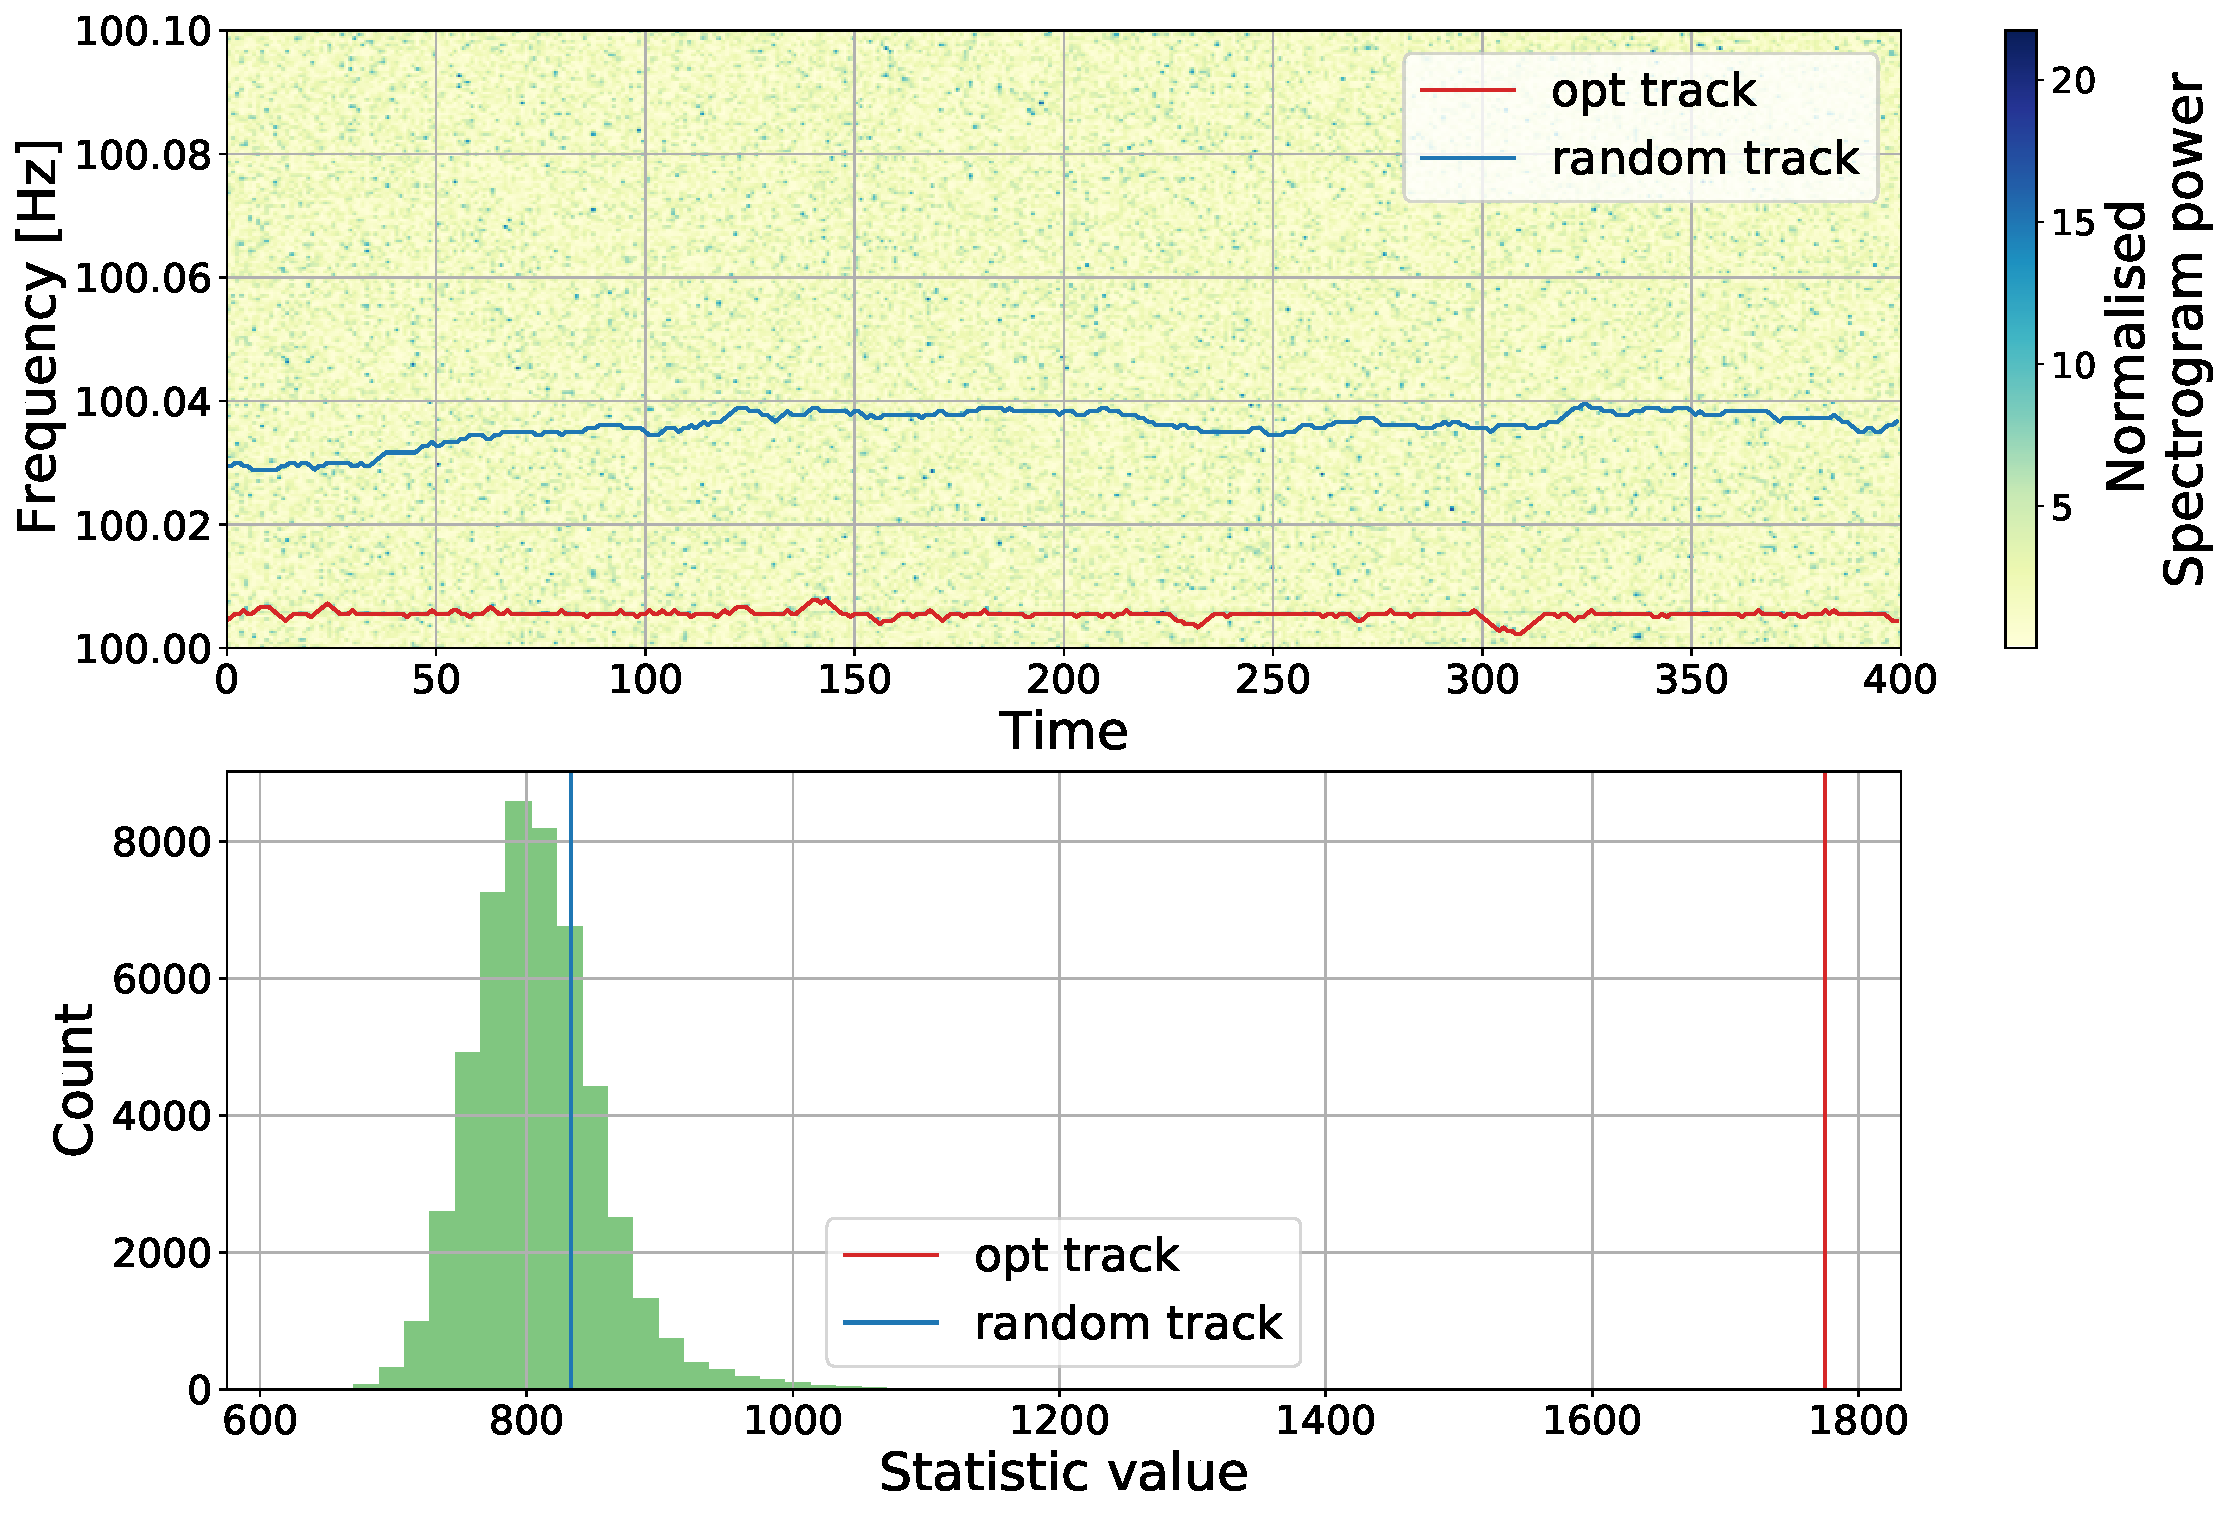
\includegraphics[width=\linewidth]{C3_soap/soap_spect_motivation.pdf}
\caption[Example of frequency tracks through a spectrogram and their summed power.]{This figure shows an example of a time-frequency spectrogram which is typical of \gls{LIGO} data which is searched through. Here an instrumental line has been injected at 100.006 Hz. The white track shows a random walk track though this spectrogram whereas the red line shows the track which gives the highest sum of detector power. The second panel shows a histogram of a subset of all paths which can be found through the given spectrogram from start to finish. This is a subset as the total number of paths is too large to calculate. The value of the statistic which comes from the optimal path is $\sim1700$. This is much larger than any of the random tracks in our subset and much larger than the mean of all tracks. }
\label{soap:motivation:plot}

\end{figure}

\section{Introduction}

%
% introduce the signal
%
One of the main targets for current ground based \gls{GW} detectors, including \gls{LIGO}~\citep{abbott2009LIGOLaser, aasi2015AdvancedLIGO} and Virgo~\citep{acernese2008StatusVirgo, acernese2015AdvancedVirgo}, are sources of continuous gravitational waves. These are long-duration, quasi-monochromatic  sinusoidal signals that are well-modelled by a Taylor series expansion in the signal phase. A likely source of such signals are rapidly spinning non axisymmetric neutron stars.  A number of possible emission mechanisms are outlined in~\citep{prix2009GravitationalWaves,owen2009ProbingNeutron}.

%
% introduce semi-coherent search algorithms
%
These types of \glspl{GW} are expected to give strain amplitudes that are significantly below the detector's noise spectral density, and need sensitive search algorithms for detection. The most sensitive method is to use a coherent matched filter which requires knowledge of the waveform beforehand such that it can be coherently correlated with the data. This approach is used in searches for gravitational signals from known pulsars such as~\citep{dupuis2005BayesianEstimation,astone2010MethodDetection,schutz1998DataAnalysis,collaboration2017FirstSearch,abbott2019SearchesGravitational}. For broad parameter space searches, where the parameters of the signal are unknown, a large number of template waveforms must be used to sufficiently cover the parameter space.  This approach rapidly becomes computationally impractical as the search space grows, so semi-coherent search methods have been developed to deliver the maximum overall sensitivity for a given computational cost. Semi-coherent searches break the data up into sections of either time or frequency and perform a coherent analysis on these sections separately. These intermediate results can then be recombined incoherently in a number of different ways to form the final search result outlined in ~\citep{creighton2000SearchingPeriodic,abbott2019AllskySearch} and references therein.


%
% introduce SOAP
%
The analysis that we present here is known as SOAP \citep{ellis2006SnakesPlanea} and is based on the Viterbi algorithm~\citep{viterbi1967ErrorBounds}. The algorithm models a process that has a discrete number of states at discrete time steps, and computes the set of states which gives the highest probability (suitably defined) given the data. Our implementation of SOAP is intended as a stand-alone search which is naturally non-parametric and has broad applications to both searches for known signal types and signals which have an unknown frequency evolution. The algorithm works in time-frequency plane, where our `states' are represented by the time and frequency coordinates of a potential signal. We can then find the most probable set of frequencies a possible signal could have, i.e., we can find the most probable track in frequency as a function of time. This is not the first application of the Viterbi algorithm to \gls{GW} data. Another variant of the algorithm \citep{suvorova2016HiddenMarkova} has recently been used, amongst other applications, as part of a \gls{CW} search to track a pulsar with randomly wandering spin frequency~\citep{sun2018HiddenMarkov, suvorova2017HiddenMarkov,abbott2017SearchGravitational, abbott2018SearchGravitational, sun2018ApplicationHidden}. We develop an alternative version which is aimed to be applied more generally to search for any long duration signals using just \glspl{SFT}.

%
% describe the paper structure
%
In the next section we will describe the Viterbi algorithm and the basic SOAP implementation to \gls{GW} time-frequency data. We then describe additional features to the algorithm, including the use of data from multiple detectors. As well as this we describe methods used to ignore instrumental effects in the data, such as incoherently summing data and a `line aware' statistic. In the final section as well as a test of the computational cost of the search, we show results of a search performed on datasets of increasing complexity: Gaussian noise with no gaps (i.e., contiguous in time), Gaussian noise with gaps simulating real data more accurately, and finally real \gls{LIGO} data taken during the sixth science run. 


\section{\label{soap:viterbi}Viterbi algorithm}
%
% Into to viterbi
%
The Viterbi algorithm is an efficient method for determining the most probable set of states (a single `track' of steps on the time-frequency plane) in a Markov model dependent on data, where the model has a discrete number of states at each step. Rather than computing the probability of every possible track and selecting the most probable, the algorithm maximises this probability after every discrete step. As a result, a partial track which cannot ultimately be the most probable is rejected before the next step is calculated, and only a fraction of all possible tracks need to be computed to find the one that is most probable.

%
% Defining varibles and what data we use
%
In this work we apply the Viterbi algorithm to a \gls{GW} strain time-series to find the most probable track of a single variable-frequency signal in the noisy data.  We divide the time series into $N$ equal-length and contiguous segments ${\bm x}_j$,  defining the set $D \equiv \{{\bm x}_j\}$. The `states' in the model correspond to the frequencies a signal could have in each segment. A `track' is a list of such frequencies ${\bm \nu}\equiv \{\nu_j\}$, where  $\nu_j$ is the frequency in the segment ${\bm x_j}$.

%
% defining probabilities
%
Our objective is to calculate the most probable track given the data, i.e., the
track that maximises $p({\bm \nu}\mid D)$. Using Bayes theorem, this posterior probability can
be written as
%
\begin{equation}
\label{soap:viterbi:bayes}
  p({\bm \nu} \mid D) = \frac{p({\bm \nu})p(D \mid {\bm \nu})}{p(D)},
\end{equation}
%
where $p({\bm \nu}) $ is the prior probability of the
track, $p(D \mid{\bm \nu})$ is the likelihood of the track (i.e., the
probability of the data given the track) and $p(D)$ is the model evidence (or
marginalised likelihood).

The Viterbi algorithm treats the track as the result of a Markovian process,
such that the current state depends only on the previous state. It is
therefore useful to split the track's prior into a set of transition
probabilities such that
%
\begin{align}
\label{soap:viterbi:prior}
p({\bm \nu}) &= p(\nu_{N - 1}, \ldots, \nu_1, \nu_0)\nonumber \\
%&=  p(\omega_{N} \mid \omega_{N-1}, \ldots, \omega_1,\omega_0)p(\omega_{N-1} \mid \omega_{N-2}, \ldots, \omega_1,\omega_0) \ldots p(\omega_1 \mid \omega_0)p(\omega_0) \\
&= p(\nu_{N - 1} \mid \nu_{N-2})p(\nu_{N-2} \mid \nu_{N-3}) \dots p(\nu_1 \mid \nu_0)p(\nu_0) \nonumber \\
&= p(\nu_0)\prod_{j=1}^{N-1}p(\nu_{j} \mid \nu_{j-1}),
\end{align}
%
where $p(\nu_0)$ is the prior probability that the signal in the first time
step has a frequency $\nu_0$ and $p(\nu_{j} \mid \nu_{j-1})$ is the
prior `transition' probability for $\nu_j$ given the frequency at the last
step was $\nu_{j-1}$.

The noise in each of the segments can be treated as independent, so the
likelihood component in Eq.~\ref{soap:viterbi:bayes} can be factorised as
%
\begin{equation}
\label{soap:viterbi:likelihood}
p(D \mid {\bm \nu}) = \prod_{j=0}^{N-1}p({\bm x_j} \mid \nu_j),
\end{equation}
%
 where $p({\bm x_j} \mid \nu_j)$ is the likelihood of our
signal having a frequency $\nu_j$ in the $j$th segment.

Using Eqs.~\ref{soap:viterbi:bayes},\ref{soap:viterbi:prior} and
\ref{soap:viterbi:likelihood}, the posterior probability is then
%
\begin{equation}
\label{soap:viterbi:posterior}
    p({\bm \nu} | D) =
    \frac{p(\nu_0)p({\bm x_0} | \nu_0) \displaystyle\prod_{j=1}^{N-1}p(\nu_{j}
| \nu_{j-1})p({\bm x_j} | \nu_j)}{\displaystyle\sum_{S}
\left\{p(\nu_0)p({\bm x_0} | \nu_0)\displaystyle\prod_{j=1}^{N-1}p(\nu_{j} |
\nu_{j-1})p({\bm x_j} | \nu_j)\right\}} ,
\end{equation}
%
where in the denominator we must sum over all possible tracks
$S$. We require the specific track, or set of frequencies, $\hat{\bm
\nu}$ that  maximises the posterior probability. Therefore, as the denominator in Eq.~\ref{soap:viterbi:posterior} is a sum over all possible tracks, the track which maximises the posterior is the same track which
maximises the numerator  on the right-hand side of  Eq.~\ref{soap:viterbi:posterior}, i.e.,
%
\begin{equation}
\label{soap:viterbi:maxtrack}
  p(\hat{\bm \nu} | D) \propto \max_{\bm \nu}{\left[p(\nu_0)p({\bm x_0} |
\nu_0) \prod_{j=1}^{N-1}p(\nu_{j} |\nu_{j-1})p({\bm x_j} | \nu_j)\right]}.
\end{equation}
%
This track also maximises the log of the probability and can be written as,
%
\begin{equation}
\label{soap:viterbi:maxtracklog}
\begin{split}
  \log p(\hat{\bm \nu} | D)  = \max_{{\bm \nu}}{\biggl\{ \log p(\nu_0) + \log p({\bm x_0} | \nu_0)  } \\
 \left. \sum_{j=1}^{N-1} \biggl[ \log p(\nu_{j} | \nu_{j-1}) + \log p({\bm x_j}
| \nu_j) \biggr] \right\} + \text{const}.
  \end{split}
\end{equation}
%
The Viterbi algorithm finds the most probable track $\hat{\bm \nu}$ by calculating the quantities in Eq,~\ref{soap:viterbi:maxtracklog} for each frequency at each time step. In the following sections we explain how this is achieved in practice.

%%%%%%%%%%%%%%%%%%%%%%%%%%%%%%%%%%%%%%%%%%%%%%%%%%%%%%%%%%%%%%%%%%%%%%%%%
%%%%%%%%%%%%%%%%%%%%%%%%%%%%%%%%%%%%%%%%%%%%%%%%%%%%%%%%%%%%%%%%%%%%%%%%%
\section{\label{soap:viterbi:transition}The transition matrix}
%%%%%%%%%%%%%%%%%%%%%%%%%%%%%%%%%%%%%%%%%%%%%%%%%%%%%%%%%%%%%%%%%%%%%%%%%
%
% define the transition matrix
%
An important concept when using the Viterbi algorithm is the`transition matrix' $T$, which is defined as the matrix that stores the prior log-probabilities $\log p(\nu_j \mid \nu_{j-1})$. These transition probabilities depend only on the size and direction of the transition, and in our case correspond to a jump in frequency when moving from the $(j-1)$th to the $j$th state. It is within the transition matrix that we impose some loose model constraints. For example it is usual in the time-frequency plane for frequencies to only have discrete values (frequency bins) and a track might only be allowed to move by one bin in each time step, restricting it to a \gls{UCD} transition or `jump' or equivalently setting the size of the first dimension of the transition matrix $n_1 = 3$. We can also impose that the transition probabilities are independent of the current track location in frequency, i.e. $p(\nu_j \mid \nu_{j-1})=p(\nu_{j+k} \mid \nu_{j+k-1})$. This leads to the transition matrix containing only three numbers, corresponding to the three prior log-probabilities that the track was in the corresponding \gls{UCD} frequency bin at the previous time step. These numbers are chosen to reflect the prior probability of a frequency deviation in the track and depend on the class of signals that one wishes to detect.
For the majority of examples that follow, a symmetric transition matrix is used, i.e. the probability of a transition up a frequency bin is equal to the probability of a transition down a frequency bin. This allows us to parameterise the one dimensional transition matrix with a single value, this value is the ratio of the probability of a transition to the same frequency bin, to either up or down a frequency bin. 

In later sections we will consider more complex situations in which the transition matrix describes the prior probability associated with sequences of even earlier transitions (`memory') and the case where there are multiple detectors. In these cases the number of dimensions of the transition matrix can grow substantially to account for the extra complexity of the problem.

%%%%%%%%%%%%%%%%%%%%%%%%%%%%%%%%%%%%%%%%%%%%%%%%%%%%%%%%%%%%%%%%%%%%%%%%%
%%%%%%%%%%%%%%%%%%%%%%%%%%%%%%%%%%%%%%%%%%%%%%%%%%%%%%%%%%%%%%%%%%%%%%%%%
\section{\label{soap:single}Single detector}
%%%%%%%%%%%%%%%%%%%%%%%%%%%%%%%%%%%%%%%%%%%%%%%%%%%%%%%%%%%%%%%%%%%%%%%%%
%
% single detector algorithm,
%
We will first consider the simple case of a single dataset $D$, generated by a single gravitational wave detector, and consider only a one-dimensional transition matrix. We will make use of discrete Fourier transforms so that frequencies, and hence the track frequencies, are also discrete. These frequencies will be indexed by $k$ and therefore $\nu_j \rightarrow \nu_{j,k}=k(j)\Delta f$ where $\Delta f=1/T$ is the frequency bin width for a segment of duration $T$.

 The Viterbi algorithm determines the most probable track on the time-frequency plane by calculating the value of Eq.~\ref{soap:viterbi:maxtracklog} for every discrete Fourier frequency, incrementally in time. In other words, at each time segment it finds the most probable earlier track which ends at each particular frequency. On reaching the final segment it can look back to identify the most probable track connecting segment 1 to segment $N$.

There are two main components to Eq.~\ref{soap:viterbi:maxtracklog}: the transition probabilities $p(\nu_j \mid \nu_{j-1})$ and the likelihoods $p({\bm x_j} \mid \nu_j)$. The transition probabilities are pre-calculated and stored in a transition matrix according to Sec.~\ref{soap:viterbi:transition} above. To calculate the likelihood we follow the approach of~\citep{bretthorst1988BayesianSpectruma} which gives, under the assumption of a single sinusoidal signal in additive Gaussian noise in data segment ${\bm x_j}$, 

%
\begin{equation}
\label{soap:single:likelihood}
p({\bm x_j} \mid \nu_{j,k}, \sigma_{j,k}, I) \propto
\exp\left[{C(\nu_{j,k})}\right].
\end{equation}
%
where
$C_{j,k}(\nu_{j,k})$ is the Schuster periodogram normalised to the noise variance at
frequency $\nu_{j,k}$ of segment $j$. This is equivalent to the log-likelihood, and is defined as
%
\begin{equation}
\label{soap:periodogram}
C(\nu_{j,k}) \equiv C_{j,k}=  \frac{1}{\sigma_{j,k}^2}\frac{1}{N_{\rm s}}\left|\sum_{r=0}^{N_{\rm
s}-1}x_{j,r} {\rm
e}^{i\nu_{j,k} t_r}\right|^2,
\end{equation}
%
where $N_{\rm s}$ is the number of data points in each segment and $t_{r}$ is the time corresponding to $x_{j,r}$, the $r$th sample in the $j$th data segment. $\sigma_{j,k}^2$ is the noise variance and is calculated as an estimate of the noise \gls{PSD} in the $k$th sample and the $j$th data segment. It is worth noting at this point that it is also possible to write this as a likelihood ratio, and therefore write out detection statistic as a log-odds ratio, however, we will discuss this in more depth in Sec.~\ref{soap:las}. The log-likelihoods of each segment can be calculated at discrete frequencies before running the algorithm by computing the power spectra for each segment from discrete Fourier transforms of the data. In the \gls{GW} field these standard data forms are known as \glspl{SFT}.

The Viterbi algorithm records two quantities for each frequency and time bin: The first, $V_{j,k}$, contains the value defined by Eq.~\ref{soap:viterbi:maxtracklog}, which is the log-probability of the most probable path ending in position $j,k$. The second, $A_{j,k}$, is the transition, or `jump', used to achieve the most probable path. The algorithm can be divided into three main sections: initialisation, iteration and identification. These three sections are described in pseudo-code in Alg.~\ref{soap:single:algorithm} and a simple demonstration of the algorithm at work is shown in Fig.~\ref{soap:plots}.
%
%
%   pseudo algorithm
%
\begin{algorithm}
\begin{algorithmic}[1]
\STATE{Input: ${C}$, $T$} \COMMENT{log-likelihood,transition matrix}
\STATE{Output: $\hat{\bm \nu}$, $V$, $A$} \COMMENT{most probable track, track probabilities, jumps}
\STATE
\STATE{ {\it Initialisation}}
\FOR{Frequency ($\nu_{0,k}$), $k=0 \rightarrow M-1$}
    \STATE{$V_{0,k} =  { C_{0k}} $ }
    \STATE{$A_{0,k} = 0$}
\ENDFOR
\STATE
\STATE{ {\it Iteration}}
\FOR{Segment, $j=0 \rightarrow N-1$}
    \FOR{Frequency ($\nu_{j,k}$), $k=0 \rightarrow M-1$}
        \STATE{$V_{j,k} = {\max\limits_{i }  ({ C_{j,k}} + T_i + V_{j-1,j+i})}$}
        \STATE{$A_{j,k} = {\argmax\limits_{ i }  ({ C_{j,k}} + T_i + V_{j-1,j+i})}$}
    \ENDFOR
\ENDFOR
\STATE
\STATE{ {\it Identification}}
\STATE{$\hat{\nu}_{N-1} = \argmax_k (V_{N-1,k})$}
\FOR{Segment, $j=N-1 \rightarrow 0$}
	\STATE{$\hat{\nu}_j = \hat{\nu}_{j+1} + A_{j,\nu_{k+1}}$}
\ENDFOR
%
\end{algorithmic}
\caption{The Viterbi algorithm in pseudo-code. $N$ is the number of segments, $M$ is the number of frequency bins in each segment. Here the maximisations over $i$ run between $\pm (n_1-1)/2$ where $n_1$ is the size of the transition matrix. The values from Eq.~\ref{soap:viterbi:maxtracklog} are stored in $V$, and the jumps are stored in $A$. The most probable track is denoted by $\hat{\bm \nu}$.\label{soap:single:algorithm}}
\end{algorithm}
%
%
% example plot to work through
%
%
\begin{figure}
\centering
\begin{subfigure}[h]{0.8\columnwidth}
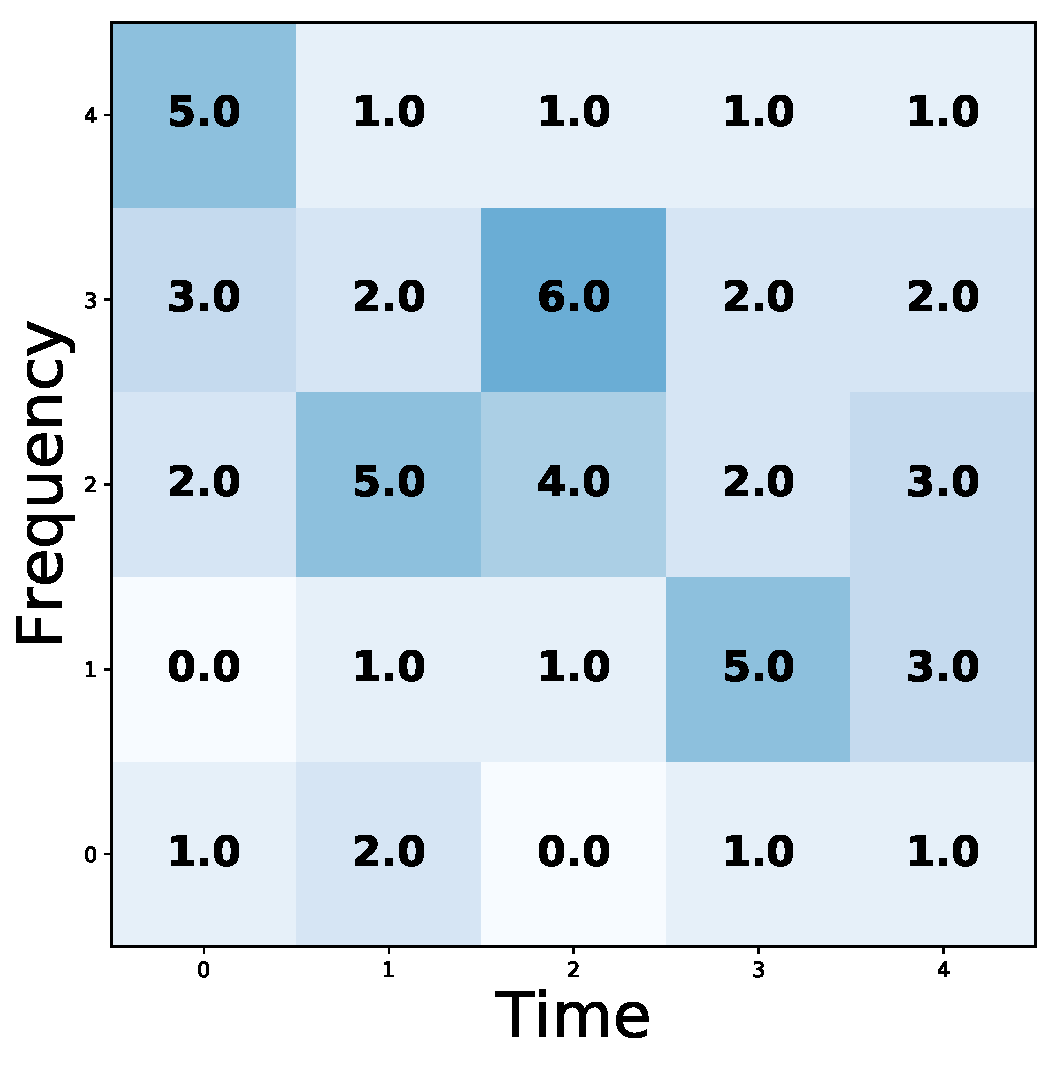
\includegraphics[width=0.8\columnwidth]{C3_soap/vit_data.pdf}
\caption{The input data}
\label{soap:plot:data}
\end{subfigure}

\begin{subfigure}[h]{0.8\columnwidth}
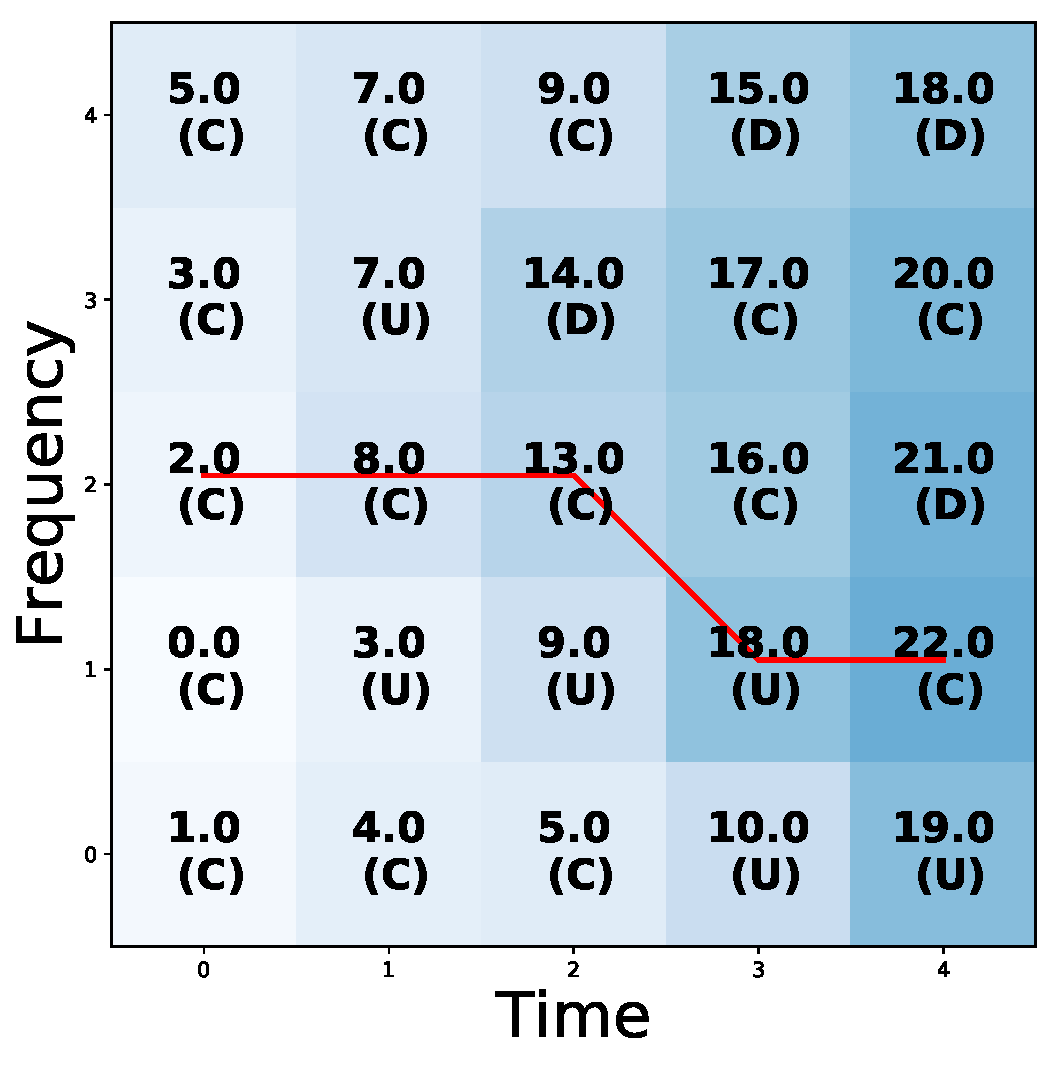
\includegraphics[width=0.8\columnwidth]{C3_soap/vit_prob.pdf}
\caption{The log-probabilities, jumps, and most probable path}
\label{soap:plot:likelihood}
\end{subfigure}

\caption[Simple example of how Viterbi algorithm works.]{ Fig.~\ref{soap:plot:data} shows
the observed data, i.e the log-likelihood values $C_{j,k}$. Fig.~\ref{soap:plot:likelihood} shows the calculated
log-probabilities $V_{j,k}$. $A_{j,k}$ is shown in parentheses, where the \gls{UCD}
components correspond to $i= [-1,0,1]$ respectively. The red line shows the
path that gives the maximum probability. The transition matrix for the \gls{UCD} jumps is $[0,1,0]$ and corresponds to the un-normalised prior
log-probabilities of these jumps occurring.}
\label{soap:plots}
\end{figure}

\begin{description}
%
% Initialisation
%
\item[Initialisation] The two parts of Eq.~\ref{soap:viterbi:maxtracklog},  $\log p(\nu_0)$ and $\log p({\bm x_0} \mid \nu_0)$, must be computed before the main recursive part of the algorithm can start. Therefore, the initialisation section (lines 5--8) in Alg.~\ref{soap:single:algorithm} calculates the first column in the lower panel of Fig.~\ref{soap:plots}. A priori, there is no preferred initial frequency, so we take the log-prior $\log p(\nu_{0,k})$ to be uniform over the complete frequency range. As a result, this is does not affect the maximisation for any jump, therefore, can be omitted from the calculation. We then use the pre-calculated log-likelihood values $C_{0,k}$ to fill the track probabilities $V_{0,k}$.  There is no previous position to jump from in this case, so the transition probabilities are irrelevant and $A_{0,k}$ are set to zero.
%
% Iteration
%
\item[Iteration] The main part of the calculation is the sum in Eq.~\ref{soap:viterbi:maxtracklog}. Lines 11--16 in Alg.~\ref{soap:single:algorithm} calculate the most probable tracks that end at each frequency bin for each segment by using
    \begin{equation} \label{soap:single:vitsum}
    V_{j,k} = \max_{i}({C_{j,k} }+ T_{i} + V_{j-1,k+i}),
    \end{equation}
    where $i$ is the size and direction of the jump. For example, in Fig.~\ref{soap:plots} columns 1--4 are calculated in order using Eq.~\ref{soap:single:vitsum}, where it maximises over three possible previous positions in frequency. These positions are the frequency bins \gls{UCD} of the current position. The size and direction of the jump, $i$, which gives the maximum probability is then saved to $A_{j,k}$. These are shown in parentheses below the log-probabilities in Fig.~\ref{soap:plots} where \gls{UCD} correspond to values of $i = [-1,0,1]$ respectively.
%
% Identification
%
\item[Identification] The final stage of the algorithm identifies the most probable track. This is done by initially finding the highest log-probability values in the final time segment, $\max_k(V_{N-1,k})$ (line 19 in Alg.~\ref{soap:single:algorithm}). In the lower panel of Fig.~\ref{soap:plots} this is located at position $j,k = 4,1$ with $V_{4,1} = 22$. To find the track which corresponds to this, the values in $A_{jk}$ are followed backwards from this position (lines 20--21). For example, in Fig.~\ref{soap:plots} the final position is $j,k = 4,1$ and $A_{j,k} = \rm{Center} = 0$, this means that at the previous segment the most probable track was at position $j,k = 4-1,1+0 = 3,1$. At this time $A_{3,1} = R = 1$, therefore, the next track element is at $j,k = 3-1,1+1 = 2,2$. This then continues until $j=0$ whereupon these retraced positions constitute the most probable track, highlighted in red in Fig.~\ref{soap:plots}.
%
\end{description}

%
% mention the limitations - only returns max track.
%
The most probable track is the one traced backwards from the highest probability final segment frequency position. However, tracks can also be traced back from any of the end-frequency positions, returning the most probable track conditional on a given final position. Such tracks should not be confused with the being equal to the second, third, fourth, etc. most probable tracks. Information regarding the rankings and properties of all possible tracks (excluding the most probable and conditionally most probable tracks) is lost during the maximisation procedures computed at each stage in the algorithm --  a necessary consequence of the algorithm's speed and efficiency.

%%%%%%%%%%%%%%%%%%%%%%%%%%%%%%%%%%%%%%%%%%%%%%%%%%%%%%%%%%%%%%%%%%%%%%%%%
%%%%%%%%%%%%%%%%%%%%%%%%%%%%%%%%%%%%%%%%%%%%%%%%%%%%%%%%%%%%%%%%%%%%%%%%%
\section{\label{soap:multidet}Multiple detectors}
%%%%%%%%%%%%%%%%%%%%%%%%%%%%%%%%%%%%%%%%%%%%%%%%%%%%%%%%%%%%%%%%%%%%%%%%%
%
% introduce what multidetector means
%
If there are $Q$ detectors operating simultaneously we have $Q$ sets of data which can be combined appropriately to provide input to the Viterbi search described above. We must also modify the allowed transitions encoded within the transition matrix to take account of the extra prior constraints that are now available.

%
% Doppler shift at each detector
%
The received instantaneous frequency of a given astrophysical signal will be nearly the same for all ground-based \gls{GW} detectors, and our
algorithm should be sensitive to tracks that show this consistency in
frequency. However there \emph{will} be small differences between the frequencies measured at detectors that are not co-located, due to differential Doppler shifts caused by Earth rotation. As a result the signal could fall in different frequency bins at each detector.

\iffalse
To sufficient accuracy, the difference in frequency $\Delta f^{(1,2)}$ seen by two detectors ($1$ and $2$), is simply
%
\begin{equation}
\label{soap:multidet:doppler}
\Delta f^{(1,2)} = \frac{({{\bm v}^{(1)}} -{{\bm v}^{(2)}})\cdot{\bm \theta}}{c} f_0,
\end{equation}
%
where ${\bm v}_a$ is the velocity of detector $a$ in an inertial reference frame, $\bm \theta$ is a unit vector in the direction of the source and $f_0$ is the instantaneous signal frequency in the reference frame. The maximum difference would occur for two detectors on the equator separated by 180 degrees of longitude and for a source located in the equatorial plane, giving
%
\begin{equation}
\label{soap:multidet:doppler:diff}
\Delta f_{\rm max}  \approx 3.1\times 10^{-6} f_0.
\end{equation}
%
For a signal frequency of 200\,Hz the largest possible instantaneous difference in frequency between detectors is therefore $6.2\times 10^{-4}$\,Hz.  Our standard 1800\,s-long \glspl{SFT} have a frequency bin-width of $5.6\times 10^{-4}$\,Hz, making this difference significant. As a result it is not enough to simply enforce that the signal tracks follow identical paths in the two detectors and we must allow some level of flexibility on the scale of $\pm 1$ frequency bin.~\chris{I find this paragraph a bit too specific to our analysis choices. We don't have to state the SFT length here. We can simply point out that you can tune the SFT length to give you differing probability distributions on your transition matrix elements. We've chosen to only 1800 sec SFTs and focus on 200\,Hz and therefore use 3 possibilities (UCD) but we could have used a different SFT length and frequency giving us any number of possible jumps. I think that we should make things easy for ourselves and state that we only ever consider 3 possibilities and then you simply tune the SFT length to your frequency spread.}
\fi

%
% Continue algorithm explanation
%
To account for these small differences in signal tracks in each detector, we reference the observed tracks to a third (pseudo) detector located at the centre of the Earth which would be insensitive to Earth spin. The signal frequencies in each real detector are then allowed to vary within a certain number of frequency bins from the track in the reference detector. In the examples that follow, we only consider the possibilities that the track in each real detector is no more that one frequency bin away from the reference track. We can tune the length of the \glspl{SFT} to ensure this is a valid assumption.
As well as differences in signal frequency, due to antenna patterns and other effects, the measured signal amplitude may differ between the detectors. In the following example we assume that the signal has the same amplitude in each detector, however, in Sec.~\ref{soap:las} we discuss the case where they differ.

We will now show how the algorithm in Sec.~\ref{soap:single} can be modified to handle a two-detector network (i.e., $Q=2$),  however any number of detectors can easily be accommodated. In the two detector case the joint probability of two (real) tracks, $\nu^{(1)}$ and $\nu^{(2)}$, and the geocentric track $\nu$, given the data, is
%
\begin{equation}
\begin{split}
p(\nu,\nu^{(1)},\nu^{(2)} | D^{(1)},D^{(2)}) \propto p(\nu)p(\nu^{(1)},\nu^{(2)} | \nu) \\
p(D^{(1)} | \nu^{(1)})p(D^{(2)} | \nu^{(2)}),
\end{split}
\end{equation}
%
where $D^{(1)}$ and $D^{(2)}$ represent the data from the two detectors. The
main difference between this and that described in Sec.~\ref{soap:single} is
that the track probabilities $V_{j,k}$ are stored for the geocentric
pseudo-detector. The main iterative calculation (defined for the single
detector case in Eq.~\ref{soap:single:vitsum}) now becomes
%
\begin{equation}
\label{soap:multidet:vitsum}
  V_{j,k} = \max_{i,l,m}({C}^{(1)}_{j,k+l} + {C}^{(2)}_{j,k+m} + T_{i,l,m} +V_{j-1,k+i}),
\end{equation}
%
where ${C}^{(1)}$ and ${C}^{(2)}$ refer to the log-likelihoods in detectors 1 and 2 respectively and the transition matrix $T$ is an $n_1\times n_2 \times n_3$ matrix, where $n_1$ dimension refers to the jump from the previous time step, $n_2$ and $n_3$ refer to the relative frequency positions in each real detector. The transition matrix is now three-dimensional and holds the prior log-probabilities of $p(\nu)$ and $p(\nu^{(1)},\nu^{(2)} | \nu)$.  We now need to maximise over three indices: $i,l$ and $m$. The index $i$ refers to the size and direction of the jump at the geocentre (as before). The indices $l$ and $m$ refer to the number of frequency bins by which the two real tracks deviate from the geocentre track. For example, if the most probable track in the geocentred detector is in bin $j,k = 5,12$ and the values of $i,l,m = 0,-1,1$, then detector 1 is in position $j,k={5,11}$ and detector 2 is in position $j,k={5,13}$ and the geocentred track was in the position $j,k={4,12}$ at the previous time step. As a result, the track at the geocentre is only affected by Doppler modulations from the Earth's orbit whereas the tracks in the real detectors include Doppler modulations from the Earth's spin.

%
% More details on the doppler constraints
%
At every time step the frequency bin position for each real detector is forced to be within $n_l$ or $n_m$ bins of the track in the geocentred detector, where $n_l$ and $n_m$ depend on how much each detector could possibly be Doppler shifted. As mentioned previously, we only consider the case where $n_l=1$ and $n_m = 1$,  allowing the track from each real detector to be at most one frequency bin away from the geocentred track position. While we tune the \gls{SFT} length to keep this condition for different frequencies, it is also possible to tune the values of $n_l$ and $n_m$ to get a similar effect.
%
% how do we do this in practice?
%
The implementation of the multi-detector algorithm is similar to the single detector case described in Sec.~\ref{soap:single}.  However in the single detector case there is only a single variable to be maximised over for each time-frequency bin. This variable is the frequency jump from the position in the previous segment. For the multi-detector case there are at least three variables to be maximised over: the probability of the jump, $i$, at the geo-centre and the probability of the signal being in the surrounding positions in each on $Q$ real detectors, $l,m,\dots$. The values of $i,l,m, \dots$ are then saved to $A_{j,k}$ and are ultimately used to reconstruct the most probable consistent tracks in each real detector.

%
%  algorithm explanation
%
As in Sec.~\ref{soap:single}, there are three main sections: Initialisation, iteration, and the identification. For the multi-detector case each element is modified as follows.

\begin{description}
% first step calculation
\item[Initialisation] The first-row calculation (lines 5--8) in Alg.~\ref{soap:single:algorithm}, are now modified to additionally maximise over the real detector track positions $l$ and $m$. For each time-frequency bin the maximum sum of the log-likelihoods is saved together with the frequency locations of the corresponding tracks in the real detectors. The index $i=0$ is kept constant as there is no previous position.

% all other steps calculation
\item[Iteration] To process the subsequent time segments, lines 13--14 in Alg.~\ref{soap:single:algorithm} are modified to account for two (or more) detectors. Line 13 of Alg.~\ref{soap:single:algorithm} is changed to calculate Eq.~\ref{soap:multidet:vitsum}, the log-probability of a track at the geocentre ending in bin $j,k$ given that signal is in the real detector positions of $j,k+l$ and $j,k+m$. Line 14 is then modified so that $A_{j,k}$ stores the jump values, $i$, and the real detector positions, $l$ and $m$, which returned the highest probability.

% finding the most probable track
\item[Identification] The most probable track is identified in the same way as for the single detector case, first by finding the maximum value in the final time step of $V_{j,k}$ (line 19 in Alg.~\ref{soap:single:algorithm}). The track at the geocentre can then be found by iteratively following the jump values stored in $A_{j,k}$ back from this position. The track in each of the real detectors is determined by using the values of $l$ and $m$ indices also stored in $A_{j,k}$ to find the relative position of the track in each real detector compared to the geocentre.
%
\end{description}

This method can be extended to more than two detectors by including additional datasets and expanding the corresponding number dimensions of the maximisation procedures in the iterative steps.

%%%%%%%%%%%%%%%%%%%%%%%%%%%%%%%%%%%%%%%%%%%%%%%%%%%%%%%%%%%%%%%%%%%%%%%%%
%%%%%%%%%%%%%%%%%%%%%%%%%%%%%%%%%%%%%%%%%%%%%%%%%%%%%%%%%%%%%%%%%%%%%%%%%
\section{\label{soap:memory} Memory}
%%%%%%%%%%%%%%%%%%%%%%%%%%%%%%%%%%%%%%%%%%%%%%%%%%%%%%%%%%%%%%%%%%%%%%%%%
%
% general idea of memory
%
In this section we extend the basic Viterbi algorithm to improve its sensitivity to non-stochastic signals where there is some knowledge of its frequency evolution.
We do this by including a form of `memory' and this extension applies to both the single and multiple-detector cases.
Rather than considering only the previous step in our decision-making process, we now include the previous $m+1$ steps and expand the transition matrix to include these values.
A memory of $m=0$ therefore corresponds to the methods described in previous sections.
With a non-zero memory the transition matrix can a-priori make certain sequences of jumps more probable and assign different prior probabilities for these jump sequences e.g., `up then centre' may be less preferable to `centre then centre'.
As a result we can increase the chance of the most probable track matching an expected astrophysical signal.
In a single detector search with a memory of $m=1$, if we only allow \gls{UCD} transitions, then for every frequency bin we save 3 values. These are proportional to the log-probabilities of a track coming from a \gls{UCD} bin in the previous time step, where the maximisation is over the corresponding \gls{UCD} bins two time steps back.
Eq.~\ref{soap:multidet:vitsum} then is then modified to,
%
\begin{equation}
\label{soap:memory:stat}
V_{j,k,s} = \max_{h} ({C}_{j,k} + T_{s,h} +  V_{j-1,k+s,k+s+h}),
\end{equation}
%
where $s$ and $h$ refer to the \gls{UCD} jumps at the time step $j-1$ and $j-2$ respectively.  Similar to the previous two sections, the algorithm is split into three parts: initialisation, iteration, and the track identification:

\begin{description}
% initialisation
\item [Initialisation] The initialisation process needs to populate the first $m+1$ steps before the main iteration can start. At the first time step, the elements $V_{0,k,s}$ are set to the log-likelihoods $C_{0,k}$ as in Sec.~\ref{soap:single}.  There is no previous time step, so the element $s$ is not relevant. At the second time step, $V_{1,k,s}$ is calculated using Eq.~\ref{soap:memory:stat}, where there is no maximisation over $h$, it is assumed to be $0$, or a center jump. As there is no data before $j=0$, the maximisation at this point will always return the jump which has the largest prior probability, which in this case is a center jump. Therefore, the maximisation returns the same value for all frequency bins and can be set to a center jump.

%Iteration
\item [Iteration] For all following time steps the values for each element of $V_{j,k,s}$ in Eq.~\ref{soap:memory:stat} are calculated. This quantity is proportional to the log-probability of the track ending in time-frequency bin $j,k$, which was in the previous position of $j-1,k+s$. The corresponding value of $h$ that maximised the log-probability of the track is recorded in $A_{j,k,s}$.

%Identification
\item [Identification] The most probable track is identified in a similar way to the non-memory cases, by finding the highest-valued last element, $V_{N-1,k,s}$. The values of $s$ and $h$ are then followed back to find the most probable track. As an example, let us assume the most probable track finishes in bin $j,k,s = 10,5,0$, where the value of $m$ is $A_{10,5,0} = 1 = \rm{up}$. The previous position is then $j,k,s=10-1,5+s,m =10-1,5+0,1=9,5,1$ with a value $A_{9,5,1} = 0 = \text{Center}$, and the next track position is $j,k,s=9-1,5+1,0=8,6,0$ etc. The values of $j,k$ along this track describes most probable path.
%
\end{description}

The number of elements over which one must search increases rapidly with memory length, and has a strong impact on the computational cost of the analysis. For the single detector Viterbi approach the number of calculations made is $3 \times N \times M$ if we only allow \gls{UCD} jumps, where $N$ and $M$ are the number of time are frequency bins respectively. When memory is included this increases to $3^{m+1} \times N \times M $.

%%%%%%%%%%%%%%%%%%%%%%%%%%%%%%%%%%%%%%%%%%%%%%%%%%%%%%%%%%%%%%%%%%%%%%%%%
%%%%%%%%%%%%%%%%%%%%%%%%%%%%%%%%%%%%%%%%%%%%%%%%%%%%%%%%%%%%%%%%%%%%%%%%%
\section{\label{soap:sumdata}Summed input data}
%%%%%%%%%%%%%%%%%%%%%%%%%%%%%%%%%%%%%%%%%%%%%%%%%%%%%%%
%
% describe what we propose to do with summed SFT power
%
In this section a method of incoherently-summing a set of \glspl{SFT} to increase the \gls{SNR} of a signal in a segment is outlined. To be more precise, it is actually the log-likelihoods which are summed, i.e. the quantity in Eq.~\ref{soap:periodogram}. We can write the new summed set of data $F_j$ as,
%
\begin{equation}
F_j = \sum_{i}^{N_s}C_{i,k}
\end{equation}
%
where $N_s$ is the number of \glspl{SFT} to sum together and the log-likelihood $C(\nu_{i,k})$ is defined in Eq.~\ref{soap:periodogram}.
We can see this is possible by looking at Eq.~\ref{soap:single:likelihood}, where we can use the product of likelihoods,
%
\begin{equation}
\begin{split}
p(D \mid \nu) &\propto p(x_1,x_2 \ldots x_n \mid \nu) \\
&\propto p(x_1 \mid \nu) \ldots p(x_n \mid \nu) \\
&\propto \exp{\left( \sum_i C_{j,k}\right)}.
\end{split}
\end{equation}
%
If the data contains gaps where the detector was not observing, then we fill the gaps in the power spectrum with a constant value which is the expectation value of the log-likelihood. The procedure of filling in the gaps of the data is completed before any summing.  Therefore, the data should have the same mean regardless of how much real data is in each sum. In the examples that follow, we sum the \glspl{SFT} over the length of one day.

The main motivation for summing the data is to increase the \gls{SNR} of a signal in the segments. The risk is that a signal can move between adjacent frequency bins during a day. To reduce this risk, we choose the frequency bin width such that it is more likely that a signal will be contained within a single frequency bin that cross a bin edge. In practise, to ensure that this is true, the segment or \gls{SFT} length and the number of segments which are summed can be tuned for each search. As well as increasing the \gls{SNR}, summing over one day should average out the antenna pattern. This means that the log-likelihood value in any bin should be more similar between detectors, however, there is still some variation due to the sky localisation and polarisation.

This also has two main effects on the transition matrix, the first is that as each segment of data is now one day long, a jump between frequency bins is far more likely, therefore, the transition matrix elements are modified to account for this. The second is that as the data is averaged over one day, the signal should remain is the same frequency bin between detectors, therefore, there is no longer a need for the multi-dimensional transition matrix described in Sec.~\ref{soap:multidet}.

The volume of the data is also reduced by a factor of $1/N_s$, therefore, the time taken for the algorithm to run is also reduced by the same factor.

%%%%
% EXTRA INFO NOT INCULDED AT THE MOMENT
%%%%%%%
\iffalse

Using the same example in Sec.~\ref{soap:multidet}, we have two detectors that are at opposite sides of the earth on the equator.
A signal in the equatorial plane at 150\,Hz will have a spread of frequency of $\Delta f = 3.1 \times 10^{-6} \times 150 \; \rm{Hz} = 4.7 \times 10^{-4} \; \rm{Hz}$.
This is less than the bin width of our 1800\,s \glspl{SFT} which is $5.6 \times 10^{-4} \; \rm{Hz}$.
Therefore, over the course of one day the signal should spend most of its time within one \gls{SFT} frequency bin.
For the real \gls{LIGO} detectors this will be less due to their locations, therefore, we can assume that the signal stays within one frequency bin for the duration of a day.
This then allows us to sum the \glspl{SFT} over one day, i.e. as we have 1800\,s long \glspl{SFT}, we can add every 48 together.

\fi
%%%%%%%

%%%%%%%%%%%%%%%%%%%%%%%%%%%%%%%%%%%%%%%%%%%%%%%%%%%%%%%%%%%%%%%%%%%%%%%%%
%%%%%%%%%%%%%%%%%%%%%%%%%%%%%%%%%%%%%%%%%%%%%%%%%%%%%%%%%%%%%%%%%%%%%%%%%
\section{\label{soap:las}Line-aware statistic}
%%%%%%%%%%%%%%%%%%%%%%%%%%%%%%%%%%%%%%%%%%%%%%%%%%%%%%%%%%%%%%%%%%%%%%%%%
%
% what is the line aware statistic
%
The multiple-detector algorithm described in Sec.~\ref{soap:multidet} returns the most probable track of a common signal assumed to be in Gaussian noise. As a consequence the algorithm will return large values of the log-likelihood even if there are inconsistent values of \gls{SFT} power between the detectors, either from non-Gaussian noise or because the signal is not equally strong in the two detectors. However a signal with unequal power in the two detectors is more likely to be a non-Gaussian instrumental line than an astrophysical signal. The line-aware statistic described in this section is designed to make the search more robust to such instrumental artefacts within realistic non-Gaussian data whilst maintaining sensitivity to astrophysical signals.

%
% More detail on what this is applied to
%
For most of the analysis examples presented here we use data which is the incoherent sum of 30-minute normalised \glspl{SFT} over a day (described in more detail in Sec.~\ref{soap:sumdata}). As a result the effects of the detector antenna patterns and of differential Doppler shifts are significantly reduced, and any signal should have a broadly similar summed log-likelihood in the same frequency bin in each detector. The statistic can then be modified such that we expect a similar log-likelihood in each detector.

We first consider the model of Gaussian noise with no signal present. Within
a single summed segment, the likelihood of Gaussian noise at
frequency $\nu$ is given by a $\chi^2$ distribution,
%
\begin{equation}
\label{las:central}
p(F_j|\nu_j,M_{\text{N}},I) = \frac{1}{2^{d/2}\Gamma(d/2)}F_j^{d/2 - 1}\exp{\left\{
\frac{F_j}{2}\right\}}
\end{equation}
%
where $F_j$ is the frequency domain power summed over sub-segments within a single day, as described in Sec.~\ref{soap:sumdata} and  $d$ is the number of degrees of freedom,  equal to twice the total number of summed SFTs.  $M_{\rm{N}}$ represents the model that the data is simply Gaussian noise. In the presence of a signal (model $M_{\text{S}}$), the power should follow a non central $ \chi^2 $ distribution in which the non-centrality parameter $\lambda$ is the square of the \gls{SNR}, $(\lambda = \rho_{\rm{opt}}^2 )$, i.e.
%
\begin{equation}
\label{las:noncentral}
\begin{split}
p(F_j|\nu_j,\lambda,M_{\text{S}},I) = \frac{1}{2} \exp{\left\{ -\frac{F_j+\lambda}{2}\right\}} \left( \frac{F_j}{\lambda} \right)^{d/4 - 1/2} \\
I_{d/2 -1}\left( \sqrt{\lambda F_j}\right).
\end{split}
\end{equation}
%
If a signal is present we therefore expect the \gls{SFT} powers in both detectors to follow Eq.~\ref{las:noncentral}.  Assuming for the moment that the noise variance is the same in both, we can determine the evidence for model $M_{\text{S}}$ by marginalising over $\lambda$,
%
\begin{equation}
\label{las:signal}
\begin{split}
p(F^{(1)}_{j},F^{(2)}_{j} \mid \nu_j,M_{\rm{S}},I) = \int_0^{\infty}  p(\lambda,w_{\rm_S}) \\
p(F^{(1)}_{j}|\nu_j,\lambda,M_{\text{S}},I)p(F^{(2)}_{j}|\nu_j,\lambda,M_{\text{S}},I) d\lambda.
\end{split}
\end{equation}
%
We set the prior on $\lambda$ to be an exponential distribution of width $w$, this is done somewhat arbitrarily as we expect the majority of signals to have a low \gls{SNR}. This distribution follows,
\begin{equation}
\label{las:prior}
p(\lambda,w) = \exp\left( \frac{-\lambda}{w}\right).
\end{equation}

On the other hand, if an instrumental line is present in one of the detectors we expect to see signal-like power in that detector and noise-like power in the other.  The evidence for this `line' model ($M_{\text{L}}$) is therefore
%
\begin{equation}
\label{las:line}
\begin{split}
p(F^{(1)}_{j},F^{(2)}_{j} \mid \nu_j,M_{\rm{L}},I) = \int_0^{\infty}  p(\lambda,w_{\rm_L}) \\
\left[ p(F^{(1)}_{j}|\nu_j,M_{\rm{N}},I)p(F^{(2)}_{j}|\nu_j,\lambda,M_{\rm{S}},I) \right. \\
\left. + p(F^{(1)}_{j}|\nu_j,\lambda,M_{\rm{S}},I)p(F^{(2)}_{j}|\nu_j,M_{\rm{N}},I)\right]d\lambda ,
\end{split}
\end{equation}
%
The third option to consider is the simple case of approximately Gaussian noise in both of the detectors,
%
\begin{equation}
\label{las:noise}
\begin{split}
p(F^{(1)}_{j},F^{(2)}_{j} \mid \nu_j,\lambda,M_{\rm{G}},I) = p(F^{(1)}_{j} \mid \nu_j,M_{\rm{G}},I) \\
p(F^{(2)}_{j} \mid \nu_j,M_{\rm{G}},I) .
\end{split}
\end{equation}
The posterior probability of model $M_{\text{GL}}$, which contains the probability of Gaussian noise or Gaussian noise with a line in one detector, (taken as mutually exclusive) is
\begin{equation}
\begin{split}
p(M_{\rm{GL}} \mid F^{(1)}_{j},F^{(2)}_{j},\nu_j ,I) = p(M_{\rm{G}} \mid F^{(1)}_{j},F^{(2)}_{j},\nu_j ,I) \\
+p(M_{\rm{L}} \mid F^{(1)}_{j},F^{(2)}_{j} ,\nu_j, I),
\end{split}
\end{equation}
where we assume that $M_{\rm{G}}$ and $M_{\rm{L}}$ are mutually exclusive.

%
We can now find the posterior odds ratio for the presence of a signal over noise or a line,
\begin{equation}
\label{soap:las:odds}
\begin{split}
O_{\rm{SGL}}(F^{(1)}_{j},F^{(2)}_{j}\mid\nu_j) &=  \frac{p(M_{\rm{S}} \mid F^{(1)}_{j},F^{(2)}_{j} ,\nu_j)}{p(M_{\rm{GL}} \mid F^{(1)}_{j},F^{(2)}_{j},\nu_j)}
= \frac{p(M_{\rm{S}} \mid F^{(1)}_{j},F^{(2)}_{j} ,\nu_j)}{p(M_{\rm{G}} \mid F^{(1)}_{j},F^{(2)}_{j} ,\nu_j) +p(M_{\rm{L}} \mid F^{(1)}_{j},F^{(2)}_{j} ,\nu_j)}\\
&=\frac{p(M_{\rm{S}})p(F^{(1)}_{j},F^{(2)}_{j} \mid M_{\rm{S}},\nu_j)}{p(M_{\rm{G}})p(F^{(1)}_{j},F^{(2)}_{j}\mid M_{\rm{G}},\nu_j) + p(M_{\rm{L}})p(F^{(1)}_{j},F^{(2)}_{j}\mid M_{\rm{L}},\nu_j) } \\
&= \frac{p(F^{(1)}_{j},F^{(2)}_{j} \mid M_{\rm{S}},\nu_j)p(M_{\rm{S}})/p(M_{\rm{G}})}{p(F^{(1)}_{j},F^{(2)}_{j}\mid M_{\rm{G}},\nu_j) + p(F^{(1)}_{j},F^{(2)}_{j}\mid M_{\rm{L}},\nu_j)p(M_{\rm{L}})/p(M_{\rm{N}}) }
\end{split}
\end{equation}
In practice it is convenient to use the log odds ratio,
\begin{equation}
\begin{split}
\label{soap:las:logodds}
\log\left[ O_{\rm{SGL}}(F^{(1)}_{j},F^{(2)}_{j})\right] &=  \log\left[ p(F^{(1)}_{j},F^{(2)}_{j} \mid M_{\rm{S}}) \right] \\
&- \left[ \log\left( p(F^{(1)}_{j},F^{(2)}_{j}\mid M_{\rm{G}}) \right. \right. \\
&\left.\left.+  p(F^{(1)}_{j},F^{(2)}_{j}\mid M_{\rm{L}})p(M_{\rm{L}})/p(M_{\rm{G}})\right) \right]
\end{split}
\end{equation}
As we are only interested in the maximum of $\log\left[ O_{\rm{SGL}}(F^{(1)}_{j},F^{(2)}_{j})\right]$, the factor $\log\left[ p(M_{\rm{S}})/p(M_{\rm{G}})\right]$ can be dropped from the expression.


In this version of the Viterbi algorithm, rather than storing a value proportional to the log-probabilities as in Sec.~\ref{soap:multidet}, here we store a value proportional to the log-odds ratio.
Here we take the log-odds ratio defined in Eq.~\ref{soap:las:logodds}, which is the log-odds of a signal having a similar power in each detector, and add the log-prior odds $p(\bm{\nu} \mid M_S)/(p(\bm{\nu} \mid M_N) + p(\bm{\nu} \mid M_L))$ which is the log-prior or any particular track. By assuming that the track transitions for the line and noise model are equally probable for any jump, we set the denominator of the prior-odds is a constant $b$.
This then means Eq.~\ref{soap:multidet:vitsum} is modified to,
\begin{equation}
\begin{split}
\label{lineaware:stat}
\hat{V}_{i,j} = \max_{k,l,m}\left(T_{k,l,m} + b + V_{i-1,j+k}   \right. \\
 + \left.  \log\left[O_{\rm{SGL}}\left(F^{(1)}_{j},F^{(2)}_{j}\right)\right]\right),
\end{split}
\end{equation}
%
where $\hat{V}$ refers to a log-odds ratio.
The maximised statistic now has three tuneable parameters: the width, $w_S$ in Eq.~\ref{las:prior}, on the prior for a signal \gls{SNR} squared, $p_{\rm S}(\lambda)$, the width, $w_L$ of the prior in the case of a line, $p_{\rm L}(\lambda)$, and the ratio of the prior on the line and noise models, $p({M_{\rm L}})/p({M_{\rm G}})$.  These parameters are optimised for each search, where we initially estimate the \gls{SNR} of a signal we hope to be sensitive to in each time slice, then use this as a guide for the width of the signal prior. This is then repeated for an expected line \gls{SNR} and this is used for the width of the line prior. The ratio of line and noise models runs in the range 0 to 1, we set this limit as we do not expect an instrumental line to be as likely as Gaussian noise in any particular frequency bin.

%
% Two detector line aware statistic
%
This line-aware statistic can be applied in a more powerful way when we use multiple detectors and is similar to the approach in \citep{keitel2014SearchContinuousa}. The multiple-detector algorithm described in Sec.~\ref{soap:multidet} returns the most probable track of a common signal assumed to be in Gaussian noise. As a consequence the algorithm will return large values of the log-likelihood even if there are inconsistent values of \gls{SFT} power between the detectors, either from non-Gaussian noise or because the signal is not equally strong in the two detectors. However a signal with unequal power in the two detectors is more likely to be a non-Gaussian instrumental line than an astrophysical signal. The line-aware statistic described in this section is designed to make the search more robust to such instrumental artefacts within realistic non-Gaussian data whilst maintaining sensitivity to astrophysical signals.

%
% More detail on what this is applied to
%
For most of the analysis examples presented here we use data which is the incoherent sum of 30-minute normalised \glspl{SFT} over a day (described in more detail in Sec.~\ref{soap:sumdata}). As a result the effects of the detector antenna patterns and of differential Doppler shifts are significantly reduced, and any signal should have a broadly similar summed log-likelihood in the same frequency bin in each detector. The statistic can then be modified such that we expect a similar log-likelihood in each detector.

In a similar way to the single-detector case, we can write out the evidence for each of the three models as follows. If a signal is present we therefore expect the \gls{SFT} powers in both detectors to follow Eq.~\ref{las:noncentral}.  Assuming for the moment that the noise variance is the same in both, we can determine the evidence for model $M_{\text{S}}$ by marginalising over $\lambda$,
%
\begin{equation}
\label{las:signal}
\begin{split}
p(F^{(1)}_{j},F^{(2)}_{j} \mid \nu_j,M_{\rm{S}},I) = \int_0^{\infty}  p(\lambda,w_{\rm_S}) \\
p(F^{(1)}_{j}|\nu_j,\lambda,M_{\text{S}},I)p(F^{(2)}_{j}|\nu_j,\lambda,M_{\text{S}},I) d\lambda.
\end{split}
\end{equation}
%
We set the prior on $\lambda$ the same as in the single detector case in Eq.~\ref{las:prior}.
In this case, if an instrumental line is present in one of the detectors we expect to see signal-like power in that detector and noise-like power in the other.  The evidence for this `line' model ($M_{\text{L}}$) is therefore
%
\begin{equation}
\label{las:line}
\begin{split}
p(F^{(1)}_{j},F^{(2)}_{j} \mid \nu_j,M_{\rm{L}},I) = \int_0^{\infty}  p(\lambda,w_{\rm_L}) \\
\left[ p(F^{(1)}_{j}|\nu_j,M_{\rm{N}},I)p(F^{(2)}_{j}|\nu_j,\lambda,M_{\rm{S}},I) \right. \\
\left. + p(F^{(1)}_{j}|\nu_j,\lambda,M_{\rm{S}},I)p(F^{(2)}_{j}|\nu_j,M_{\rm{N}},I)\right]d\lambda ,
\end{split}
\end{equation}
%
The third option is the simple case of approximately Gaussian noise in both of the detectors,
%
\begin{equation}
\label{las:noise}
\begin{split}
p(F^{(1)}_{j},F^{(2)}_{j} \mid \nu_j,\lambda,M_{\rm{G}},I) = p(F^{(1)}_{j} \mid \nu_j,M_{\rm{G}},I) \\
p(F^{(2)}_{j} \mid \nu_j,M_{\rm{G}},I) .
\end{split}
\end{equation}

%
We can now find the posterior odds ratio for the presence of a signal over noise or a line by following the same steps as in Eq.~\ref{soap:las:odds}. Once again we write this as a log-odds ratio,
\begin{equation}
\begin{split}
\label{soap:lineaware:logodds}
\log\left[ O^{(2)}_{\rm{S/GL}}(F^{(1)}_{j},F^{(2)}_{j})\right] &=  \log\left[ p(F^{(1)}_{j},F^{(2)}_{j} \mid M_{\rm{S}}) \right] \\
&- \left[ \log\left( p(F^{(1)}_{j},F^{(2)}_{j}\mid M_{\rm{G}}) \right. \right. \\
&\left.\left.+  p(F^{(1)}_{j},F^{(2)}_{j}\mid M_{\rm{L}})p(M_{\rm{L}})/p(M_{\rm{G}})\right) \right]
\end{split}
\end{equation}
The factor $\log\left[ p(M_{\rm{S}})/p(M_{\rm{G}})\right]$ can again be dropped from the expression.

For the multi-detector case we then modify Eq.~\ref{soap:multidet:vitsum} to,
\begin{equation}
\begin{split}
\label{soap:lineaware:stat:multi}
\hat{V}_{i,j} = \max_{k,l,m}\left(T_{k,l,m} + b + V_{i-1,j+k}   \right. \\
 + \left.  \log\left[O^{(2)}_{\rm{S/GL}}\left(F^{(1)}_{j},F^{(2)}_{j}\right)\right]\right),
\end{split}
\end{equation}
%
where $\hat{V}$ refers to a log-odds ratio.
This is then optimised over the same three parameters as the single detector case.

Fig.~\ref{soap:las:osgl_plots} shows an example of the output of the statistic in Eq.~\ref{soap:lineaware:logodds} for different \gls{FFT} powers $F$.
\begin{figure}
\centering

\begin{subfigure}[h]{\linewidth}
\begin{minipage}{0.65\linewidth}
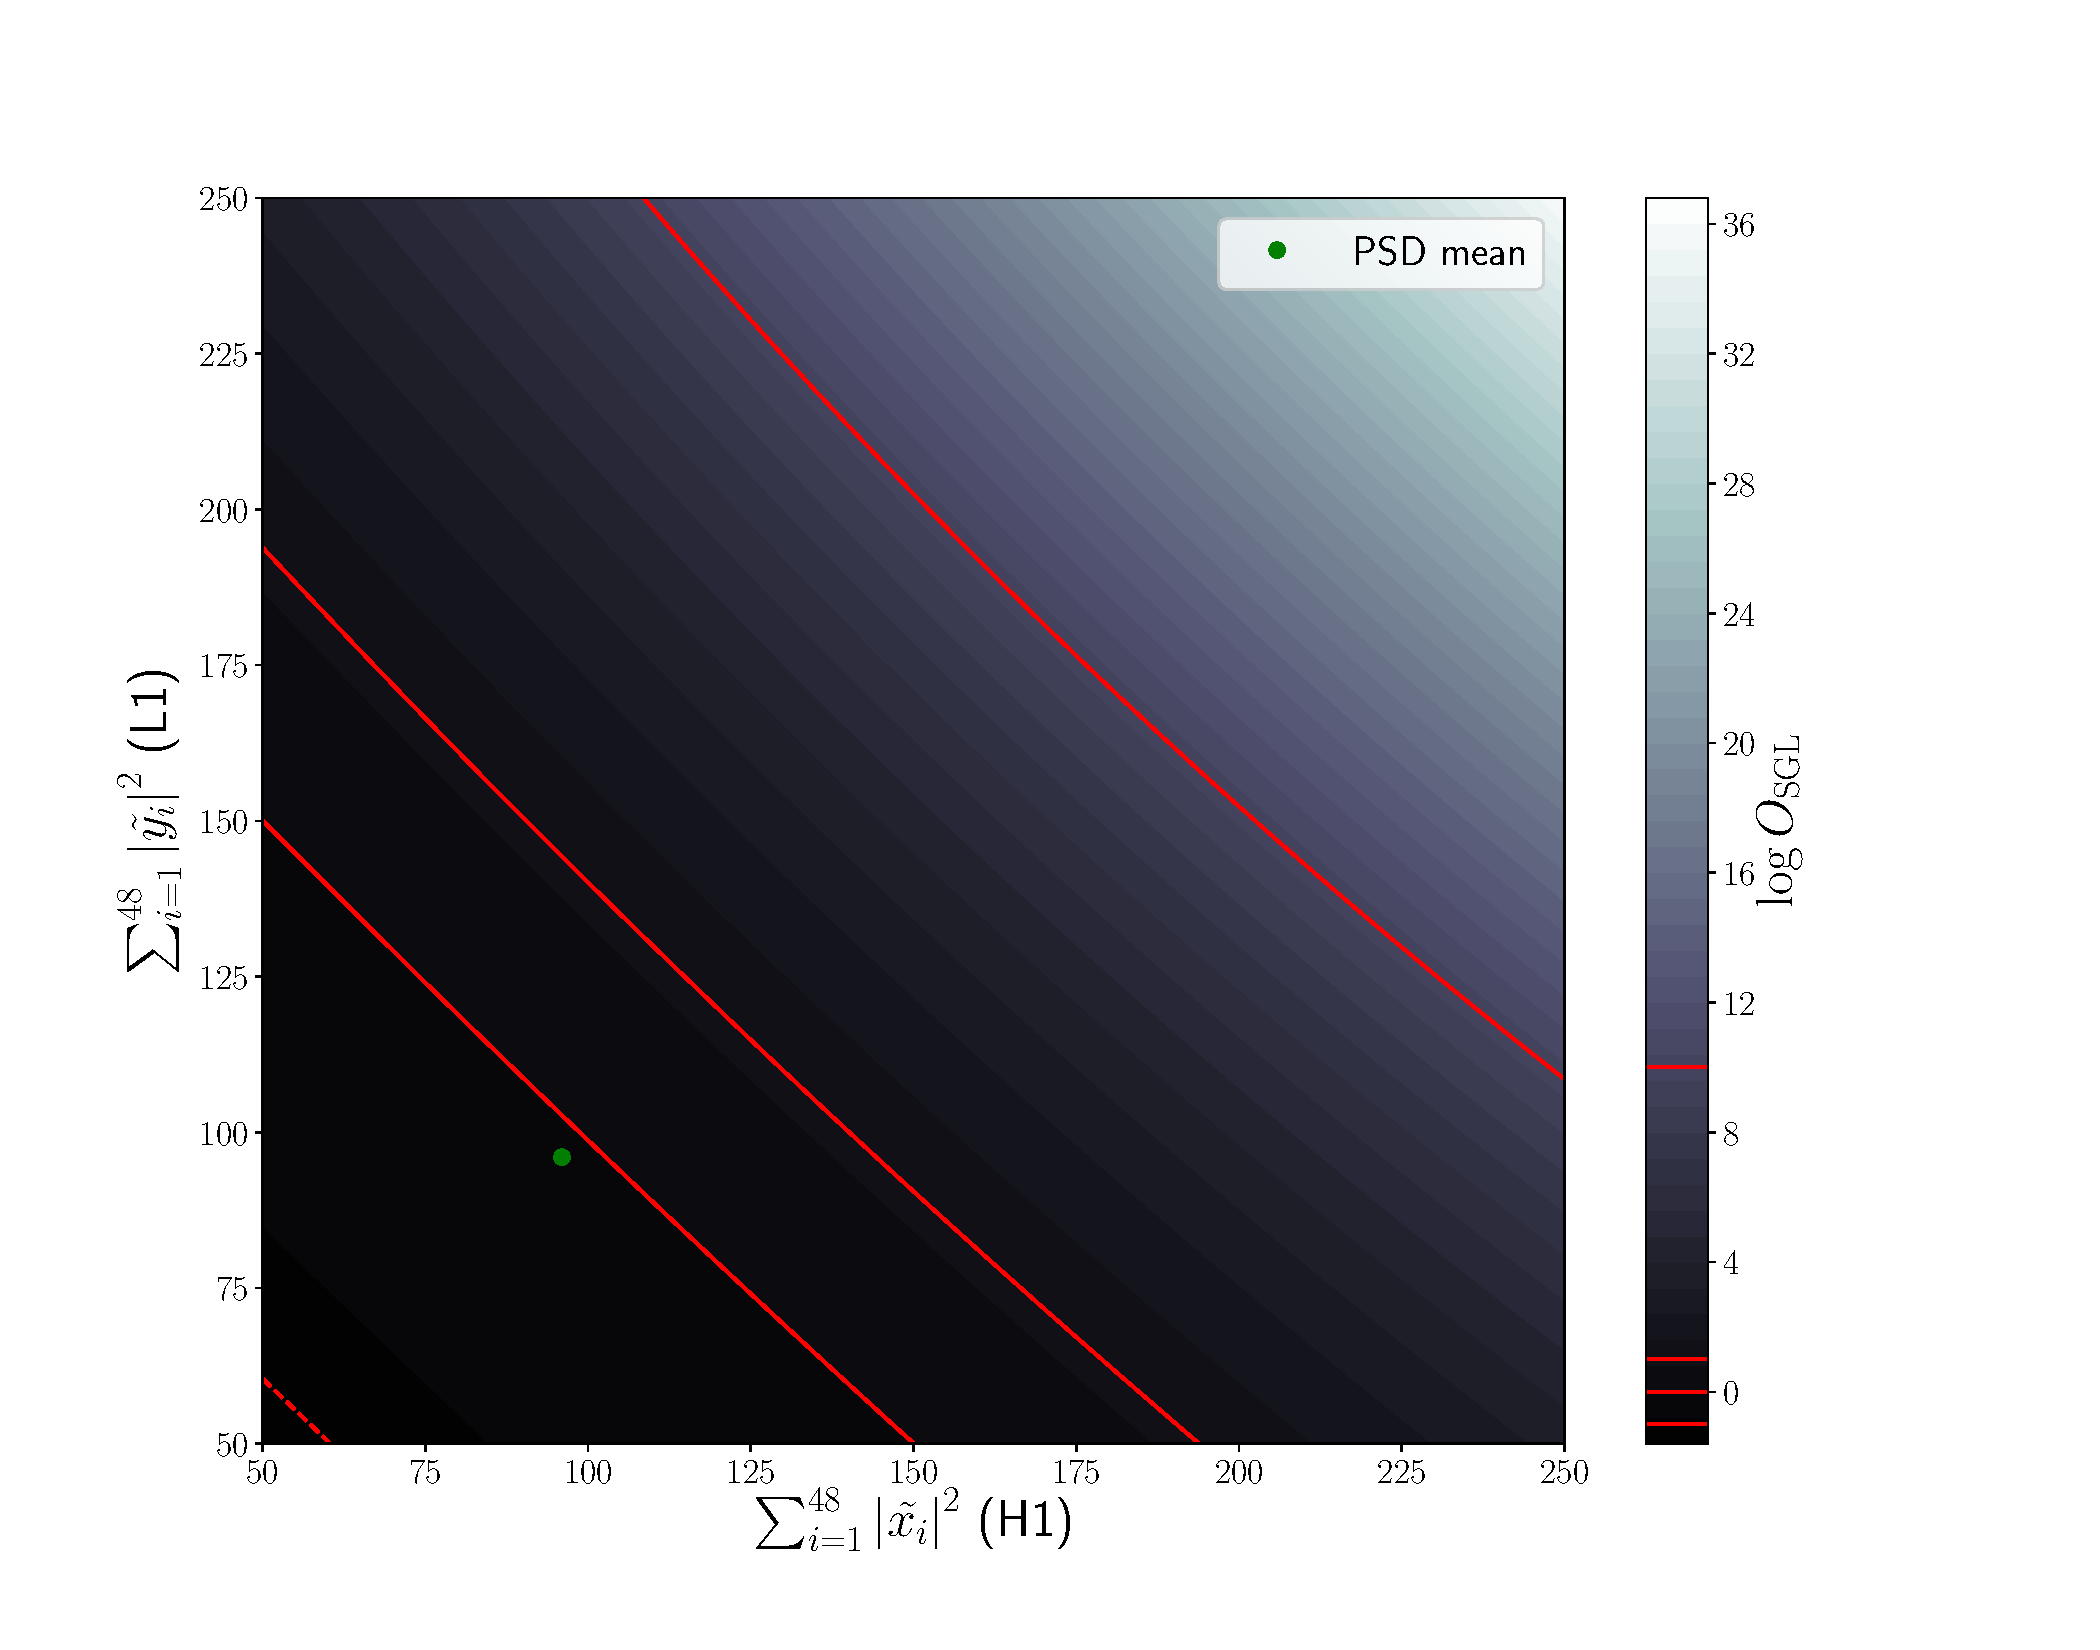
\includegraphics[width=1.\linewidth]{C3_soap/lookup_noline.pdf}
\end{minipage}\hfill
\begin{minipage}{0.35\linewidth}
\caption{This shows the distribution of the lines aware statistic plotted against the \gls{FFT} power in each detector. This example is for parameters $p_s(\lambda) = 4$,$p_l(\lambda) = 0$ and $p(M_L)/p(M_G) = 0$. So the line part of the statistic is not operating.}
\label{soap:las:detp:noline}
\end{minipage}
\end{subfigure}

\begin{subfigure}[h]{\linewidth}
\begin{minipage}{0.65\linewidth}
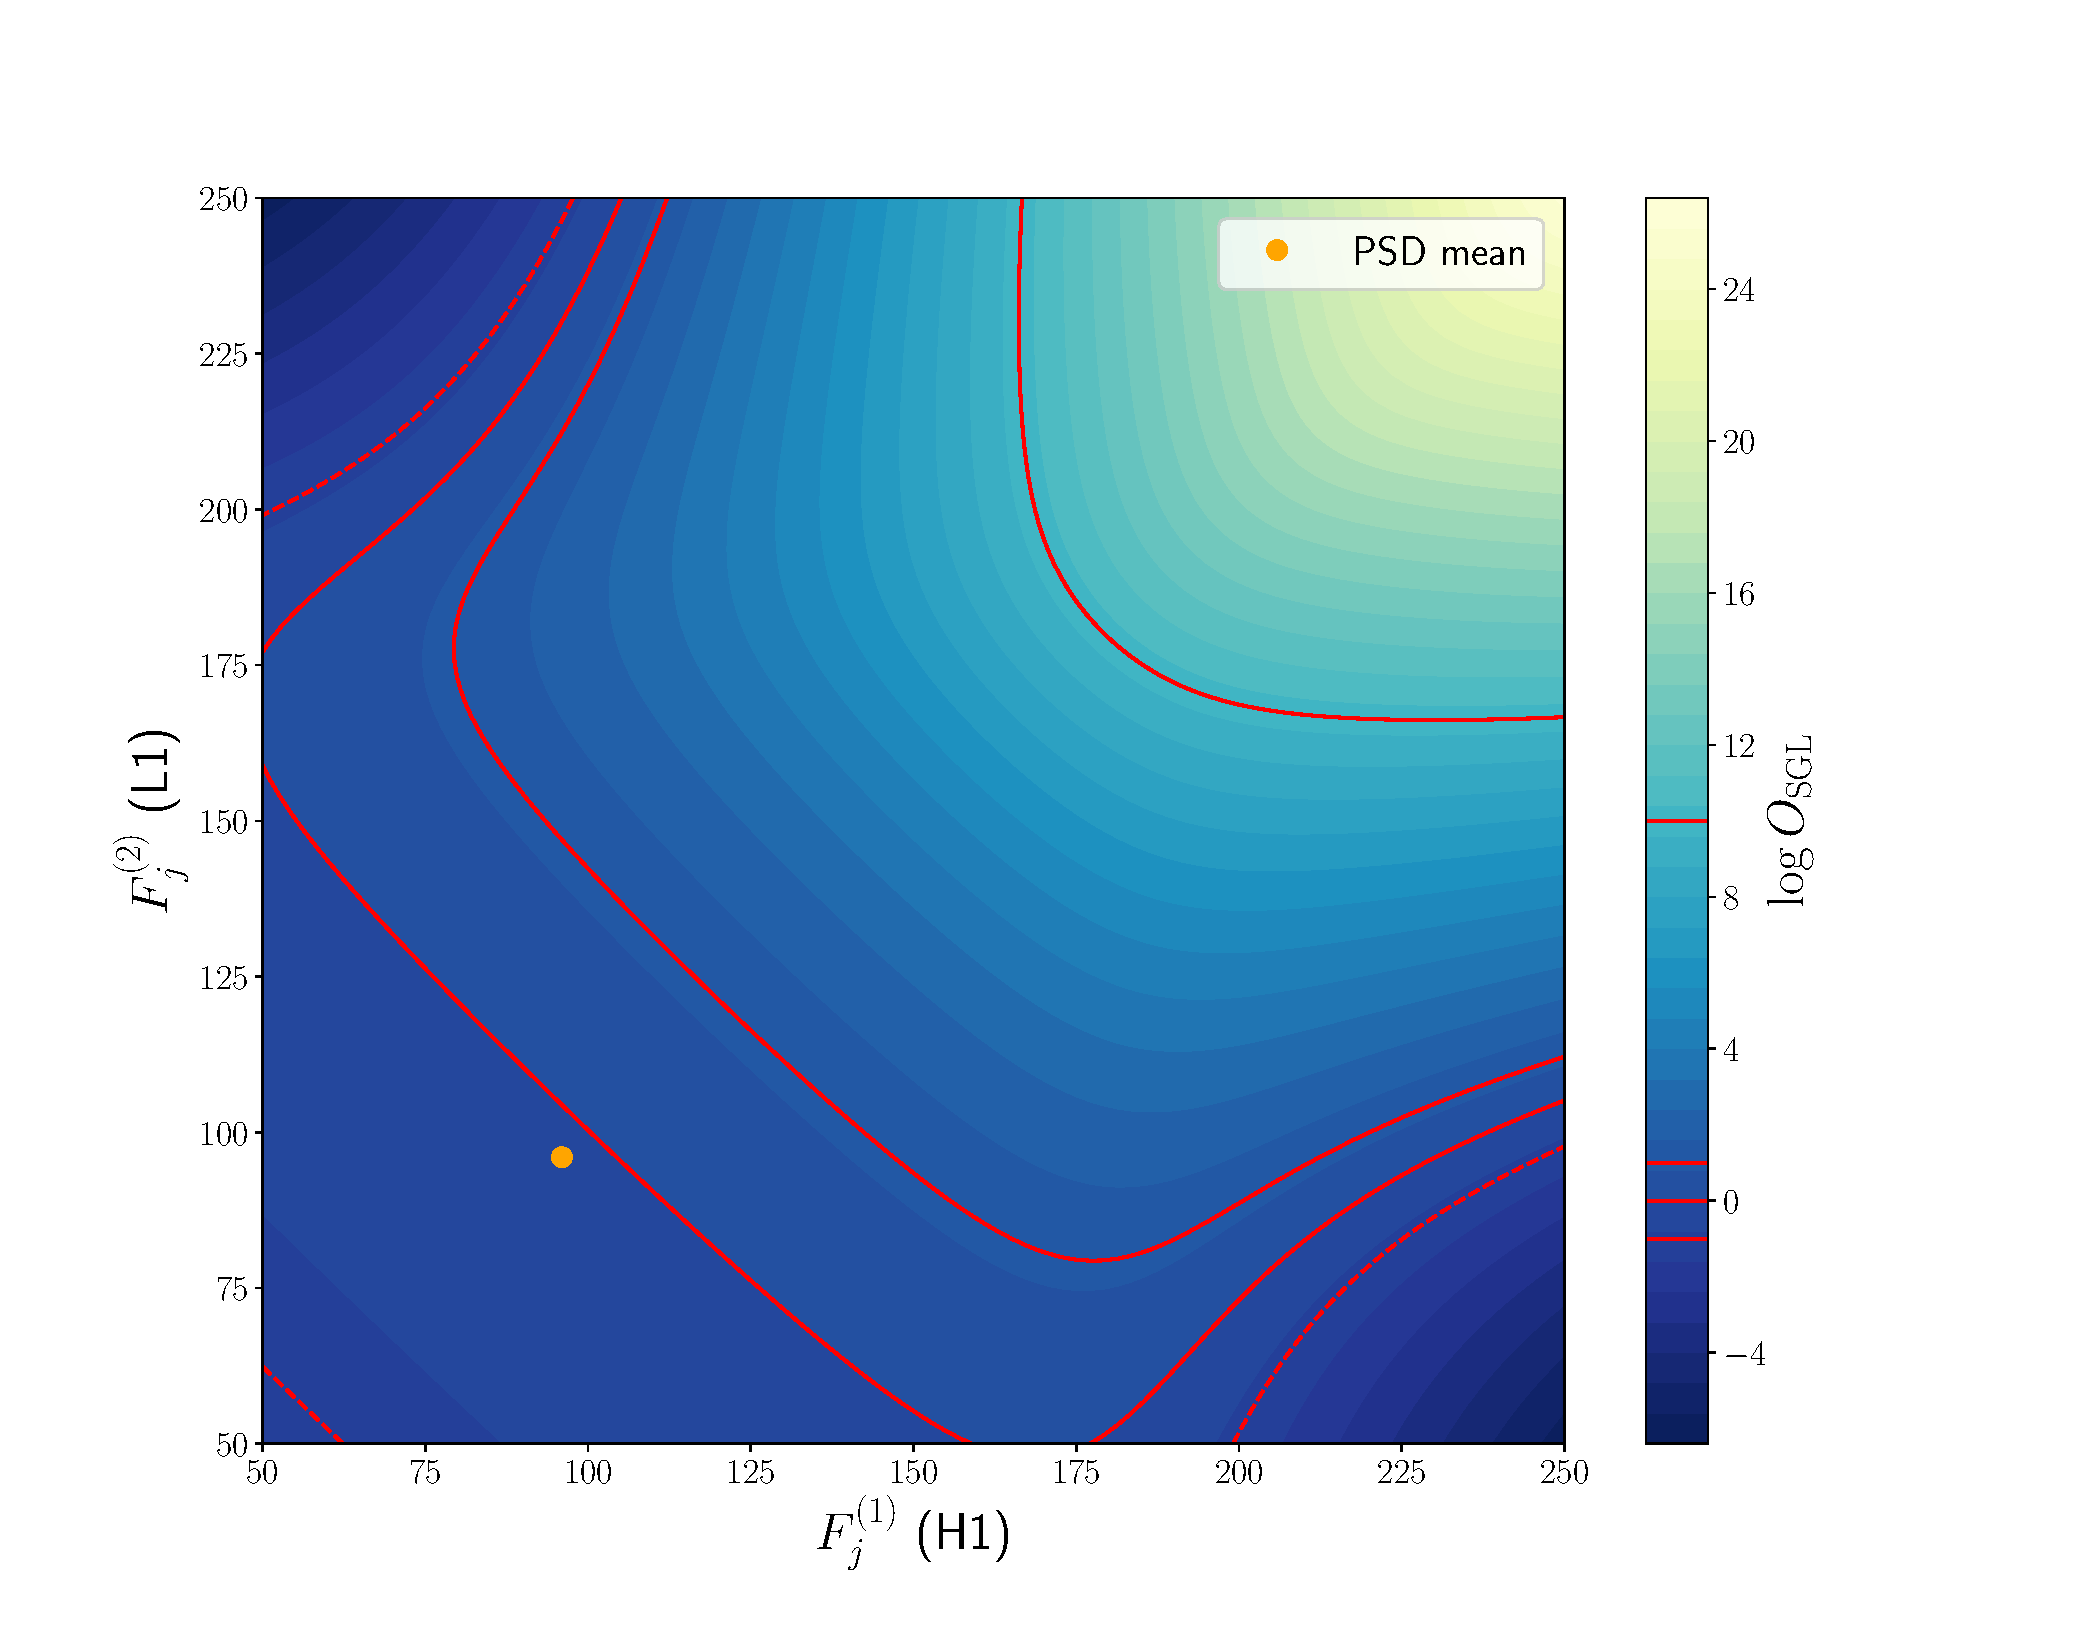
\includegraphics[width=1.\columnwidth]{C3_soap/lookup_linesmall.pdf}
\end{minipage}\hfill
\begin{minipage}{0.35\linewidth}
\caption{This shows the distribution of the lines aware statistic plotted against the \gls{FFT} power in each detector. This example is for parameters $p_s(\lambda) = 4$,$p_l(\lambda) = 5$ and $p(M_L)/p(M_G) = 0.03$. Here we include the line part of the statistic.}
\label{soap:las:detp:linesmall}
\end{minipage}
\end{subfigure}

\begin{subfigure}[h]{\linewidth}
\begin{minipage}{0.65\linewidth}
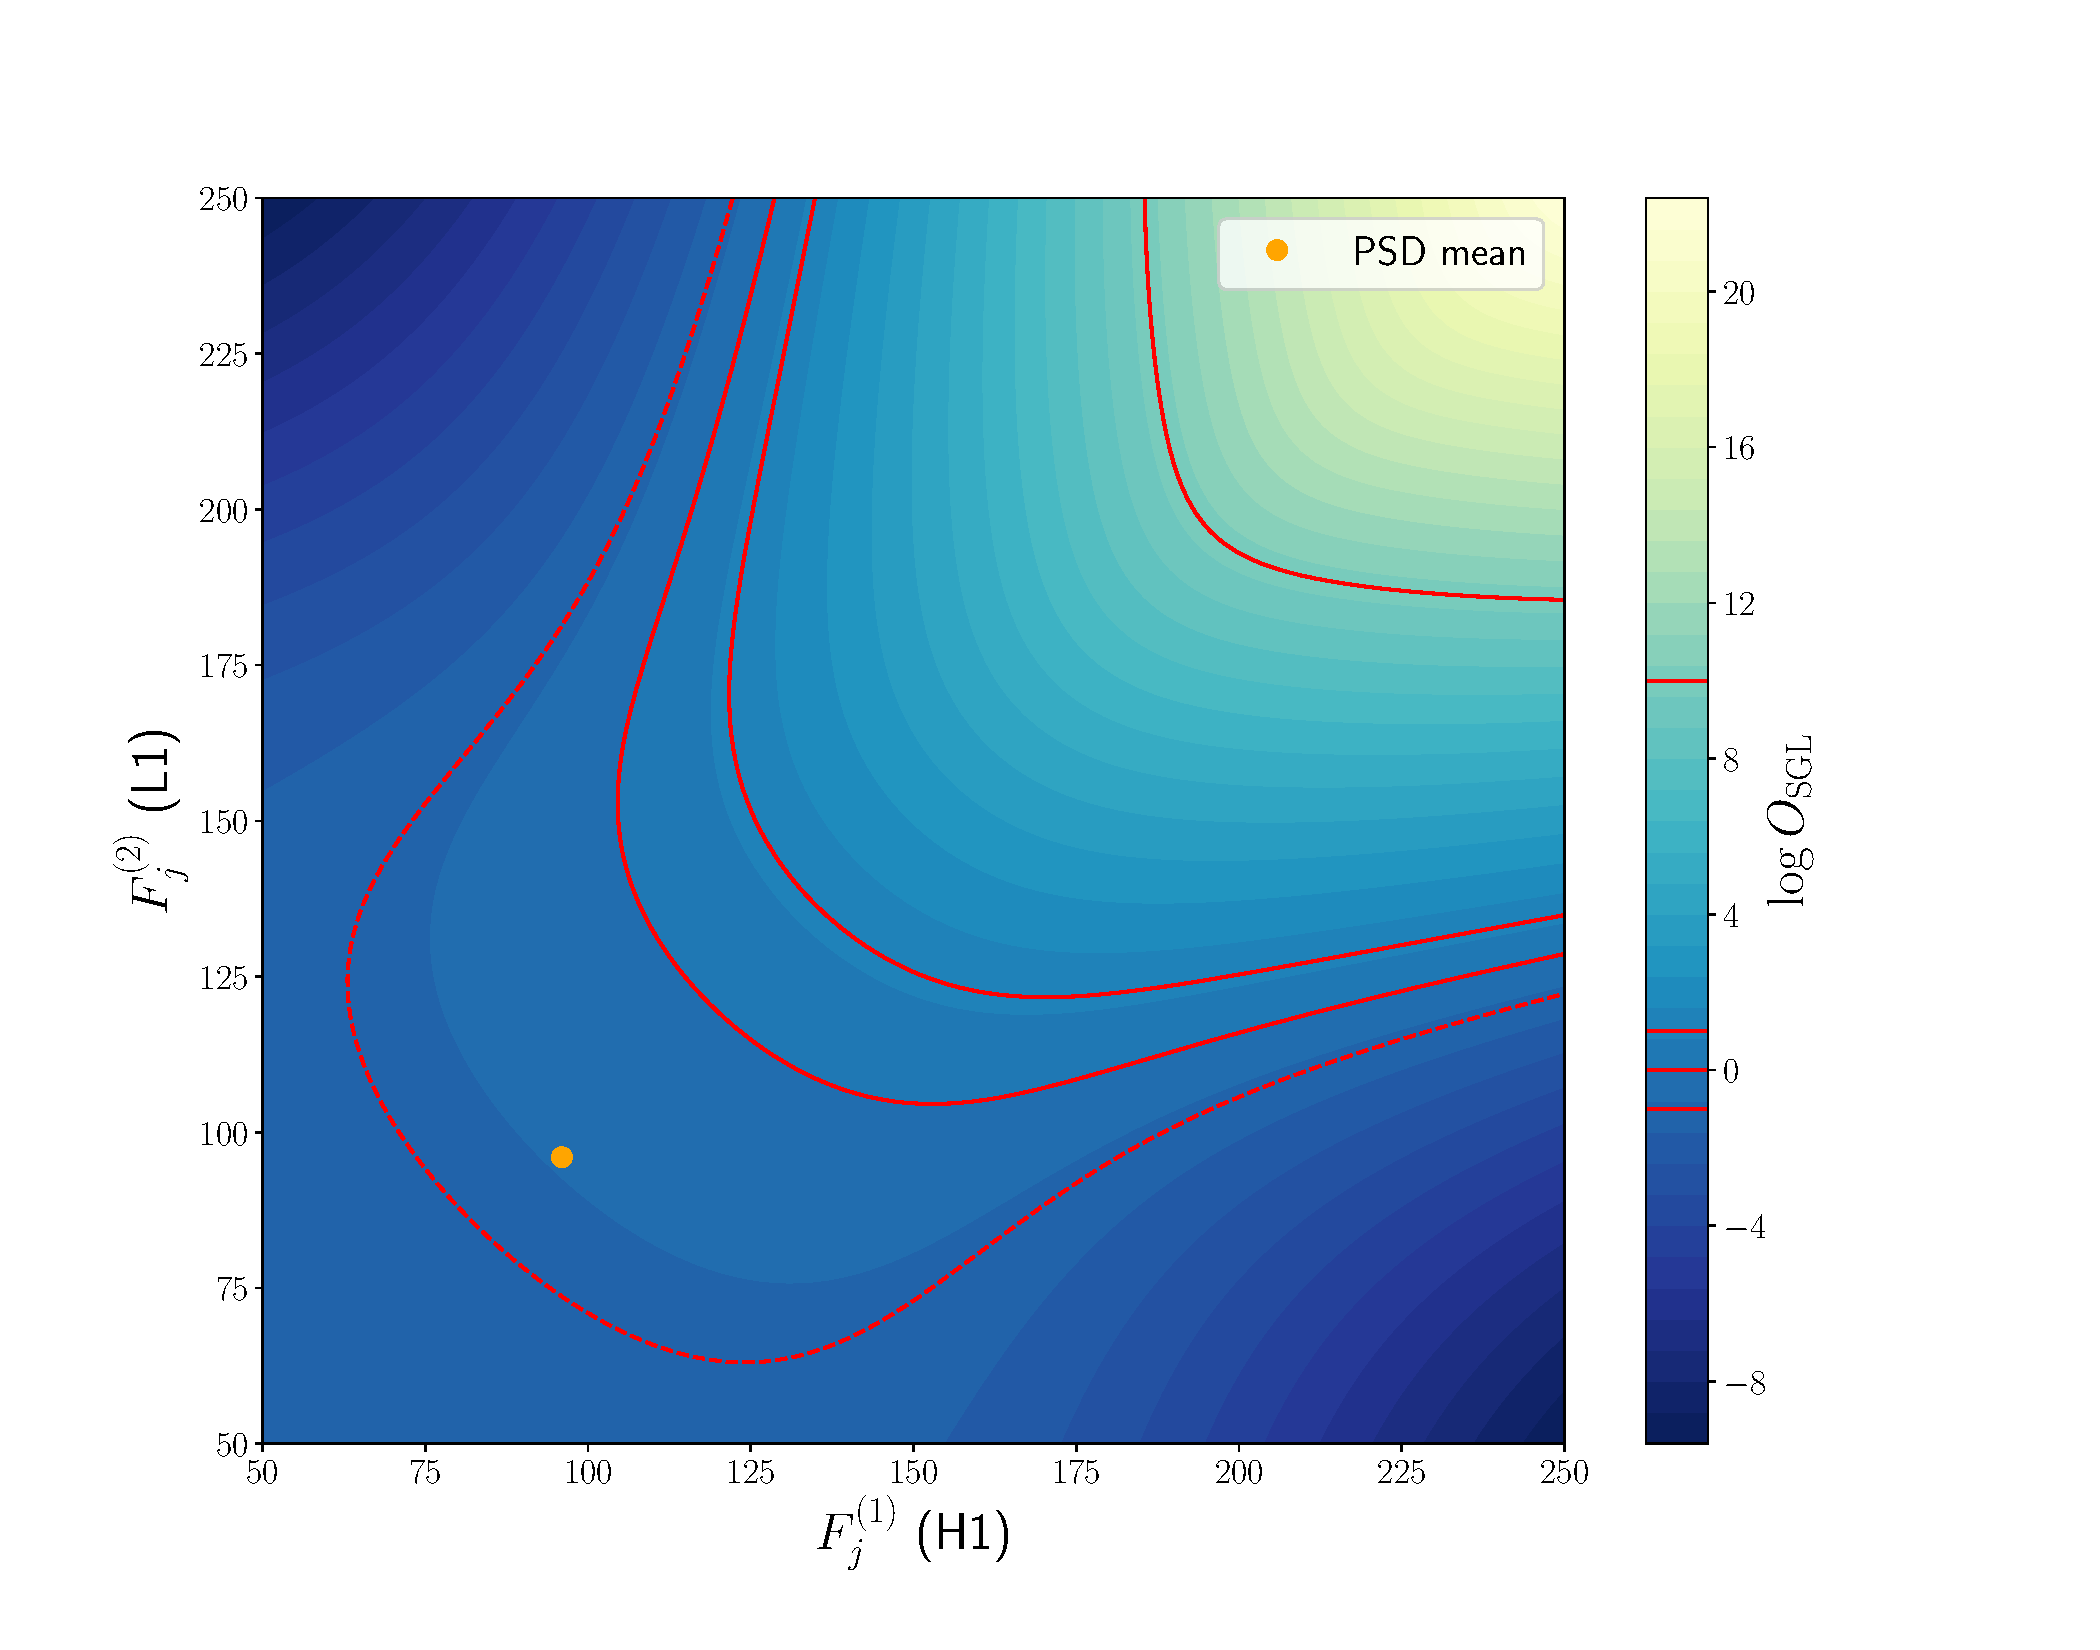
\includegraphics[width=1.\columnwidth]{C3_soap/lookup_linebig.pdf}
\end{minipage}\hfill
\begin{minipage}{0.35\linewidth}
\caption{This shows the distribution of the lines aware statistic plotted against the \gls{FFT} power in each detector. This example is for parameters $p_s(\lambda) = 4$,$p_l(\lambda) = 5$ and $p(M_L)/p(M_G) = 1$. Here the effect of lines is expected to be larger than the previous panel on the search. Therefore, the statistic forces the two detectors to have more similar power.}
\label{soap:las:detp:linebig}
\end{minipage}
\end{subfigure}
\caption[Lookup table for line aware statistic.]{Lookup tables using the line aware statistic in Eq.~\ref{soap:lineaware:stat:multi}.}
\label{soap:las:osgl_plots}
\end{figure}


%%%%%%%%%%%%%%%%%%%%%%%%%%%%%
%%%%%%%%%%%%%%%%%%%%%%%%%%%%%
\section{\label{soap:lineawareamp}Line aware statistic for consistent amplitude}
%%%%%%%%%%%%%%%%%%%%%%%%%%%%%
%%%%%%%%%%%%%%%%%%%%%%%%%%%%%


In Sec.~\ref{soap:las} the `line aware' statistic was designed to penalise high
\gls{SFT} powers in a single detector and reward powers which have a similar
\gls{SNR}. This is often a useful statistic to use when the detectors have
similar sensitivities, however, this is not always the case. During an
observing run of a gravitational wave detector, their sensitivity will vary
with time due~\chris{typo} fluctuating or new noise sources or
potentially~\chris{grammar} upgrades which
can increase the sensitivity. A change in the sensitivity, or noise floor,
affects the \gls{SNR} of a possible signal in in~\chris{typo} the data, i.e. a lower noise
floor results in a higher \gls{SNR}.  In this section the above `line aware'
statistic is modified to account for the difference in sensitivities of the
detectors, and therefore search~\chris{grammar} for a consistent amplitude between detectors as
opposed to \gls{SNR}.

There are two main factors which are taken into account when determining how
sensitive a detector is in a particular time interval: the \gls{PSD} of
detector and the duty cycle. The \gls{PSD} of the detector is
essentially~\chris{uyou shouldn't really be using words like essentially in the
thesis.} how
sensitive the detector is at that time and the duty cycle is the fraction of
time in a given interval that the detector was collecting data. A decrease in
the duty cycle and an increase in the \gls{PSD} will decrease the \gls{SNR} and
vice-versa. To search for consistent amplitude Eq.\ref{lineaware:stat} is
modified by weighting each detector by its \gls{PSD} and duty cycle.

The definition of \gls{SNR} is taken from \citep{}~\chris{missing ref} as, 
\begin{equation}
    \rho_0^2 = \frac{h_0^2 T}{S}(\alpha_1A + \alpha_2B + \alpha_3C),
\end{equation}
where $\rho_0$ is the optimal \gls{SNR}, $h_0$ is the signal amplitude, $T$ is
the time of observation, $S$ is the noise \gls{PSD} and the terms in brackets include the antenna pattern of the detector. 
The signal with amplitude $h_0$ will be the same amplitude at both detectors (H and L), therefore we can relate the \gls{SNR} in each detector by,
\begin{equation}
\label{lineawareamp:snrequate}
    \rho_L^2 = \frac{\rho_H^2 S_H T_L}{S_L T_H} \frac{(\alpha_1A_L + \alpha_2B_L + \alpha_3C_L)}{(\alpha_1A_H + \alpha_2B_H + \alpha_3C_H)} .
\end{equation}

For the majority of the analysis that follows~\chris{ideal location for a
comma} the \glspl{SFT} are summed over one day, this will~\chris{3.7 was before
this so it already has been explained} be explained in greater detail in Sec.~\ref{soap:sumdata}. 
The components in the above equation which have the form $(\alpha_1A +
\alpha_2B + \alpha_3C)$, account for the antenna pattern of the earth~\chris{of
the detector as the earth rotates} as it rotates.
These can be approximated to be the same for the two detectors H1 and L1 as we
will essentially~\chris{stop saying essentially and actually describe what is
actually being done} be0 averaging out the daily modulation by summing \glspl{SFT}.
Therefore we can simplify the above Eq.~\ref{lineawareamp:snrequate} to, 
\begin{equation}
\label{lineawareamp:snrratio}
    \rho_L^2 = \frac{\rho_H^2 S_H T_L}{S_L T_H} = l \rho_H^2 .
\end{equation}
~\chris{if it's an approximation then use $\approx$.}
This then gives a factor $l = S_H T_L/S_L T_H$ which relates the \gls{SNR} of each detector, where $S$ and $T$ are values that are known for a given data-set prior to running the search.

This ratio of \glspl{SNR} can be included in the integral over \gls{SNR} for the signal model in Eq.~\ref{las:signal} as follows,
\begin{equation}
\label{lineawareamp:signal}
p(F^{(1)}_{j},F^{(2)}_{j} \mid \nu_j,M_{\rm{S}},I) = \int_0^{\infty}  p(\lambda,w_{\rm_S}) 
p(F^{(1)}_{j}|\nu_j,\lambda,M_{\text{S}},I)p(F^{(2)}_{j}|\nu_j,l\lambda,M_{\text{S}},I) d\lambda.
\end{equation}

Similarly, the line model in Eq.~\ref{las:line} can be modified as,

\begin{equation}
\label{lineawareamp:line}
\begin{split}
p(F^{(1)}_{j},F^{(2)}_{j} \mid \nu_j,M_{\rm{L}},I) = \int_0^{\infty}  p(\lambda,w_{\rm_L}) 
\left[ p(F^{(1)}_{j}|\nu_j,M_{\rm{N}},I)p(F^{(2)}_{j}|\nu_j,l\lambda,M_{\rm{S}},I) \right. \\
\left. + p(F^{(1)}_{j}|\nu_j,\lambda,M_{\rm{S}},I)p(F^{(2)}_{j}|\nu_j,M_{\rm{N}},I)\right]d\lambda .
\end{split}
\end{equation}

Fig.~\ref{soap:lineawareamp:example} shows an example of the values of the
statistic described in Eq.~\ref{lineawareamp:line} plotted against a range of
\gls{FFT} powers from each detector. This demonstrated~\chris{use present tense} how the statistic
accounts for a difference in sensitivity on~\chris{between} detectors by allowing the \gls{FFT}
power or effectively~\chris{commas} \gls{SNR} to vary more.

In Fig.~\ref{soap:lineawareamp:example} we show an example of two detectors
with large differences in sensitivity, and how the statistic which takes this
into account can improve the search sensitivity in this case~\chris{contorted
sentence}.

\begin{figure}
\centering

\begin{subfigure}[h]{\linewidth}
\begin{minipage}{0.65\linewidth}
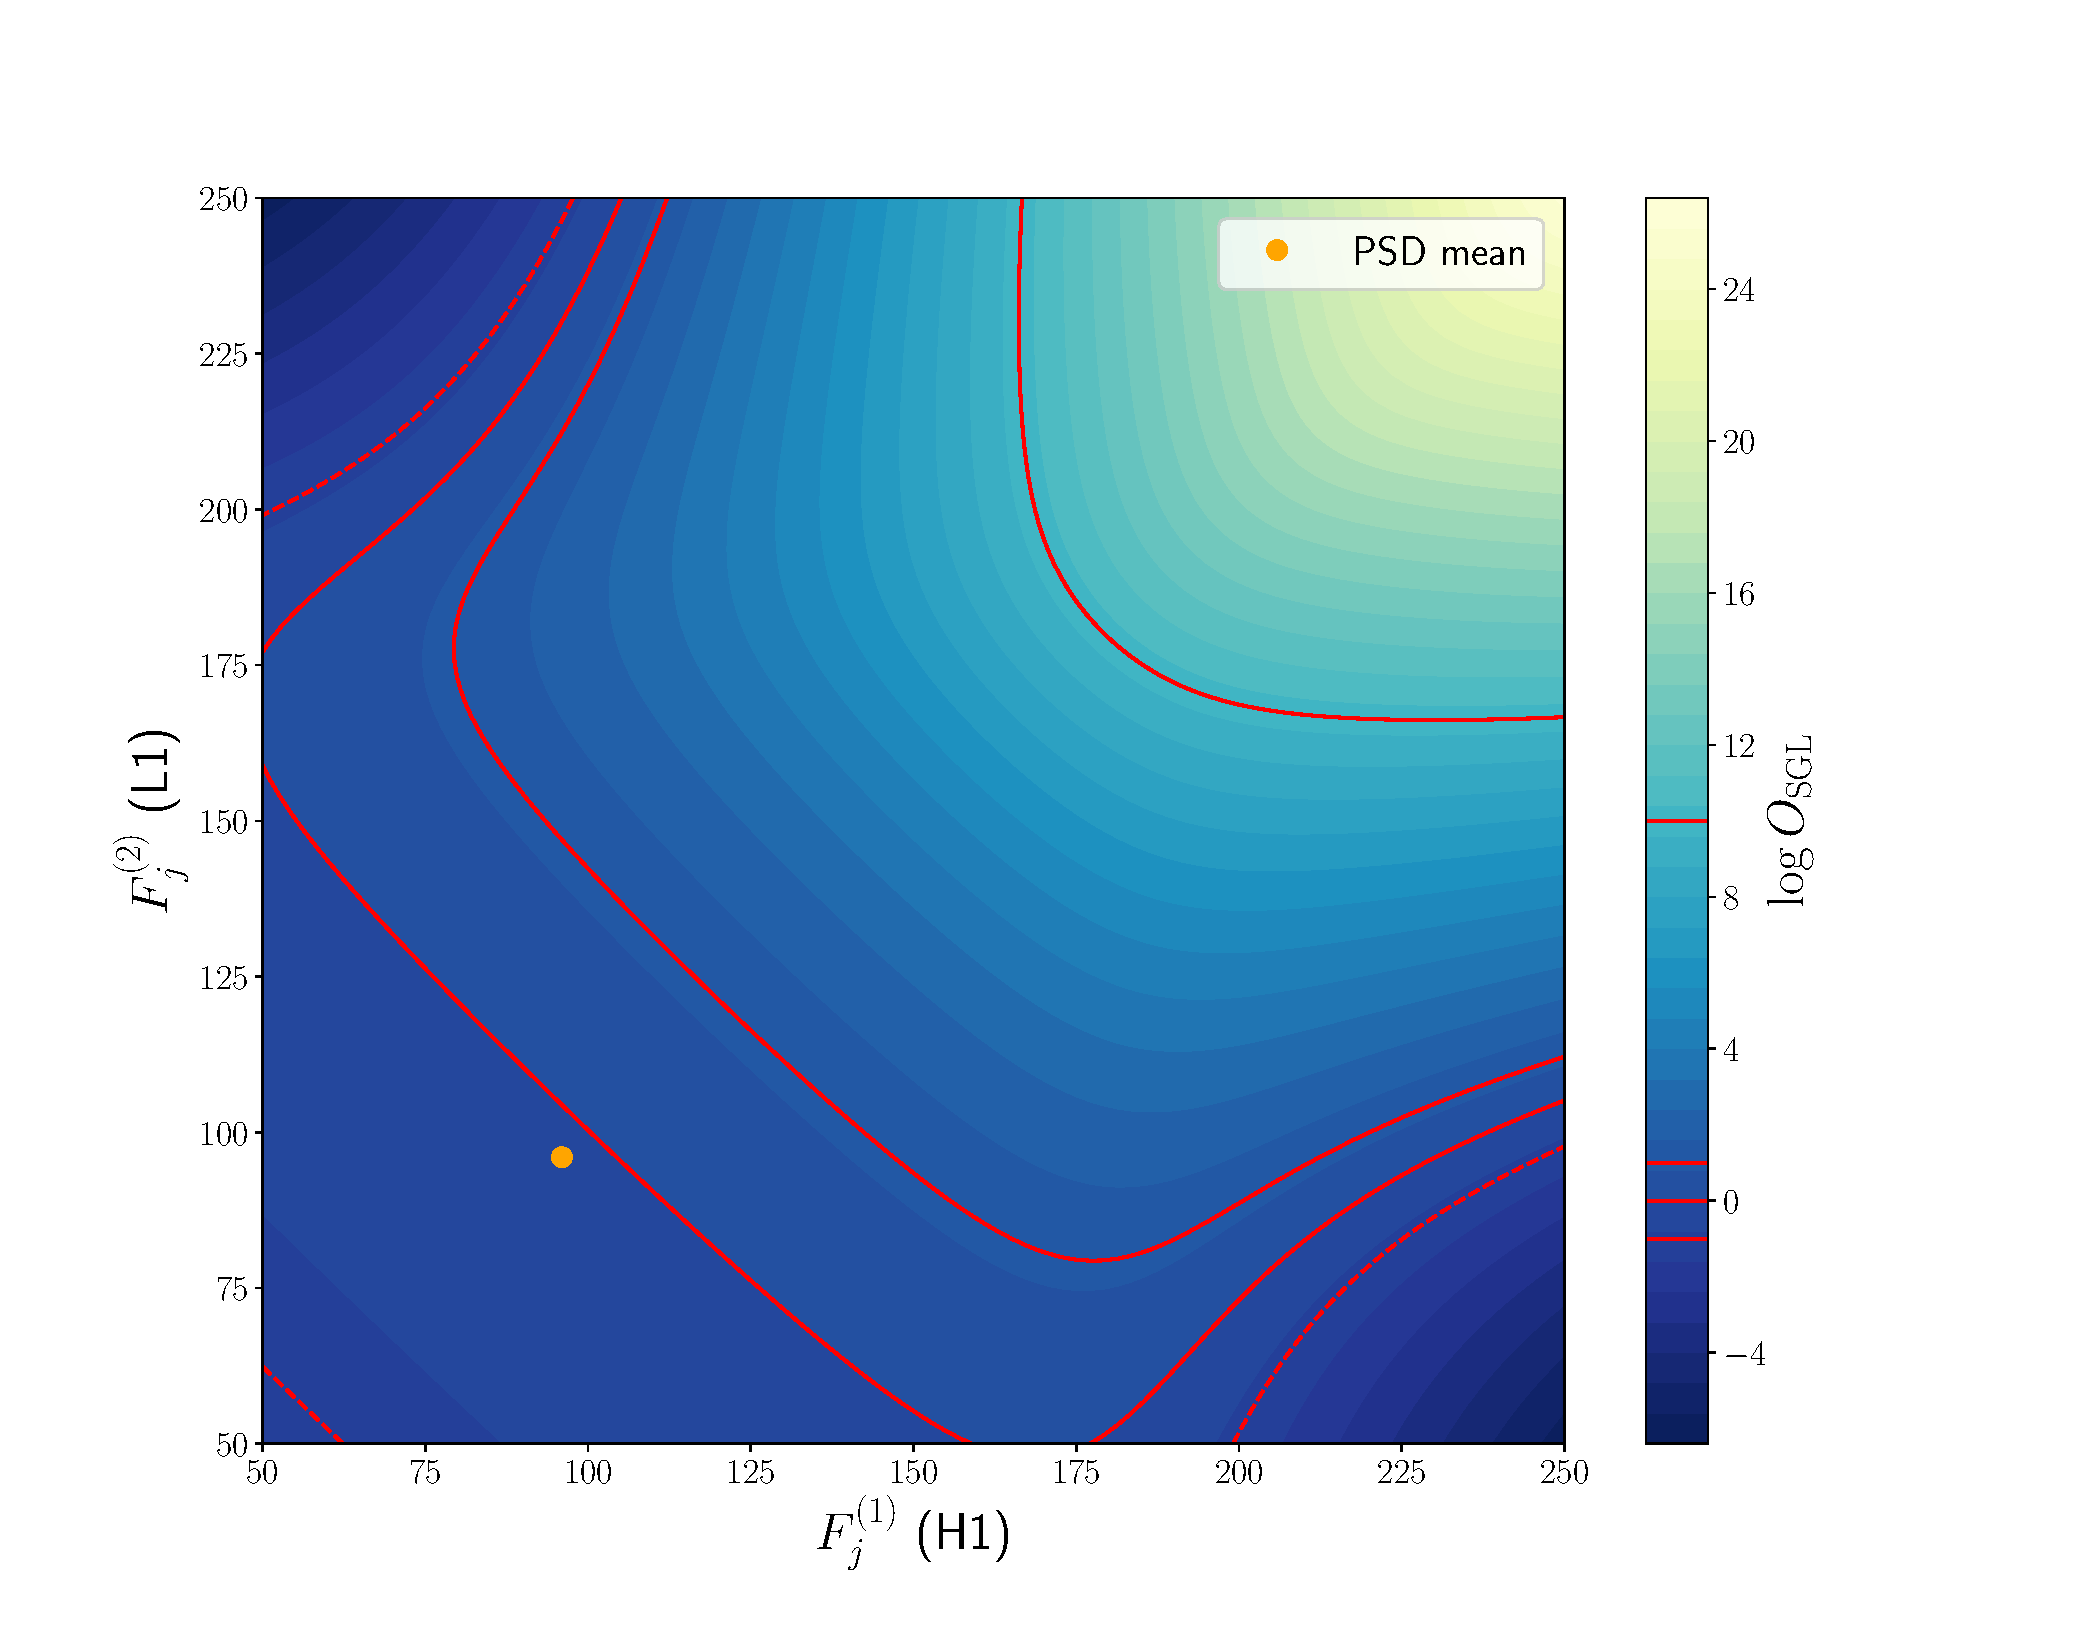
\includegraphics[width=0.9\linewidth]{C3_soap/lookup_3d_2.pdf}
\end{minipage}\hfill
\begin{minipage}{0.35\linewidth}
\caption{This shows the distribution of the lines~\chris{lines or line?} aware statistic plotted
against the \gls{FFT} power in each detector~\chris{but this is contour plot so
the LAS is not being plotted against anything. The LAS is being plotted as a
function of the input from pairs of detectors - please fix this in all panels.}. This example is for
parameters~\chris{space between equations} $p_s(\lambda) = 2$,$p_l(\lambda) =
0$ and $p(M_L)/p(M_G) = 0$. So the line part of the statistic is not
operating.~\chris{explain what PSD mean is in all these plots and are these
plots for the LAS for consistent amplitude? What is $p_{l}(\lambda)$? Has it
been defined before? }}
\label{soap:lineawareamp:plot:noline}
\end{minipage}
\end{subfigure}
\begin{subfigure}[h]{\linewidth}
\begin{minipage}{0.65\linewidth}
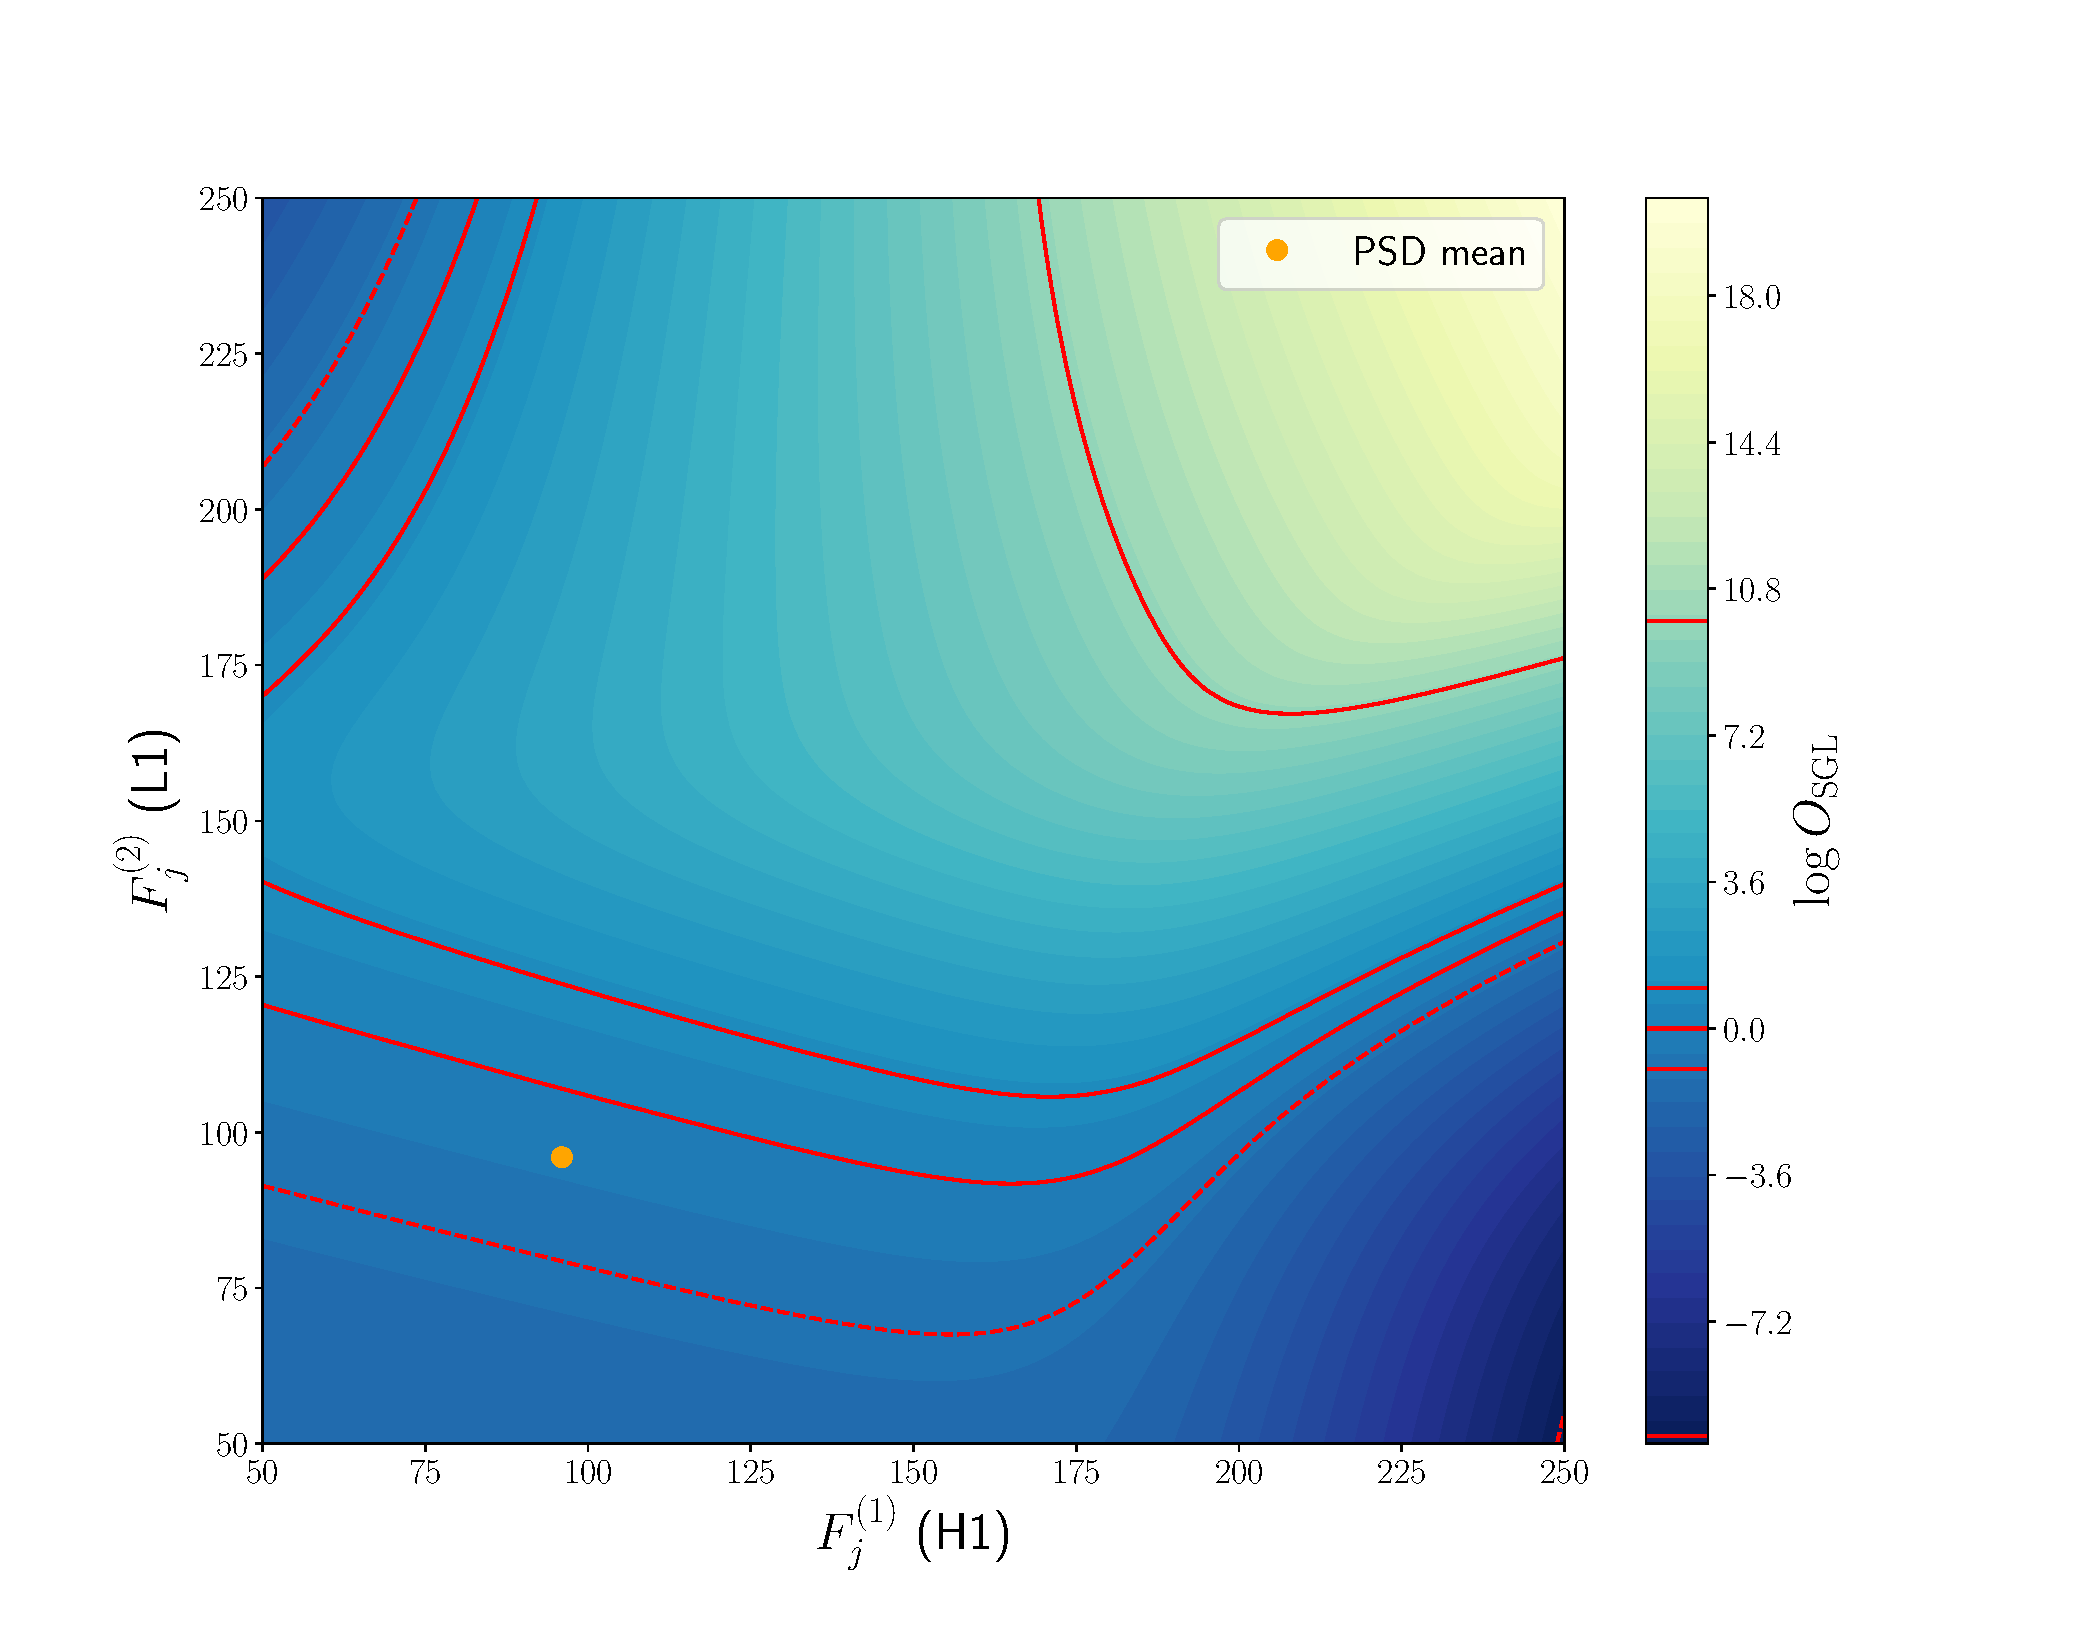
\includegraphics[width=0.9\columnwidth]{C3_soap/lookup_3d_1.pdf}
\end{minipage}\hfill
\begin{minipage}{0.35\linewidth}
\caption{This shows the distribution of the lines aware statistic plotted
against the \gls{FFT} power in each detector. This example is for parameters
$p_s(\lambda) = 2$,$p_l(\lambda) = 2$ and $p(M_L)/p(M_G) = 1$. Here the line
part of the statistic has the same \gls{SNR} and~\chris{typo} the signal part, i.e. we expect the \gls{SNR} of a signal to be similar to that of a line.}
\label{soap:lineawareamp:plot:linesmall}
\end{minipage}
\end{subfigure}

\begin{subfigure}[h]{\linewidth}
\begin{minipage}{0.65\linewidth}
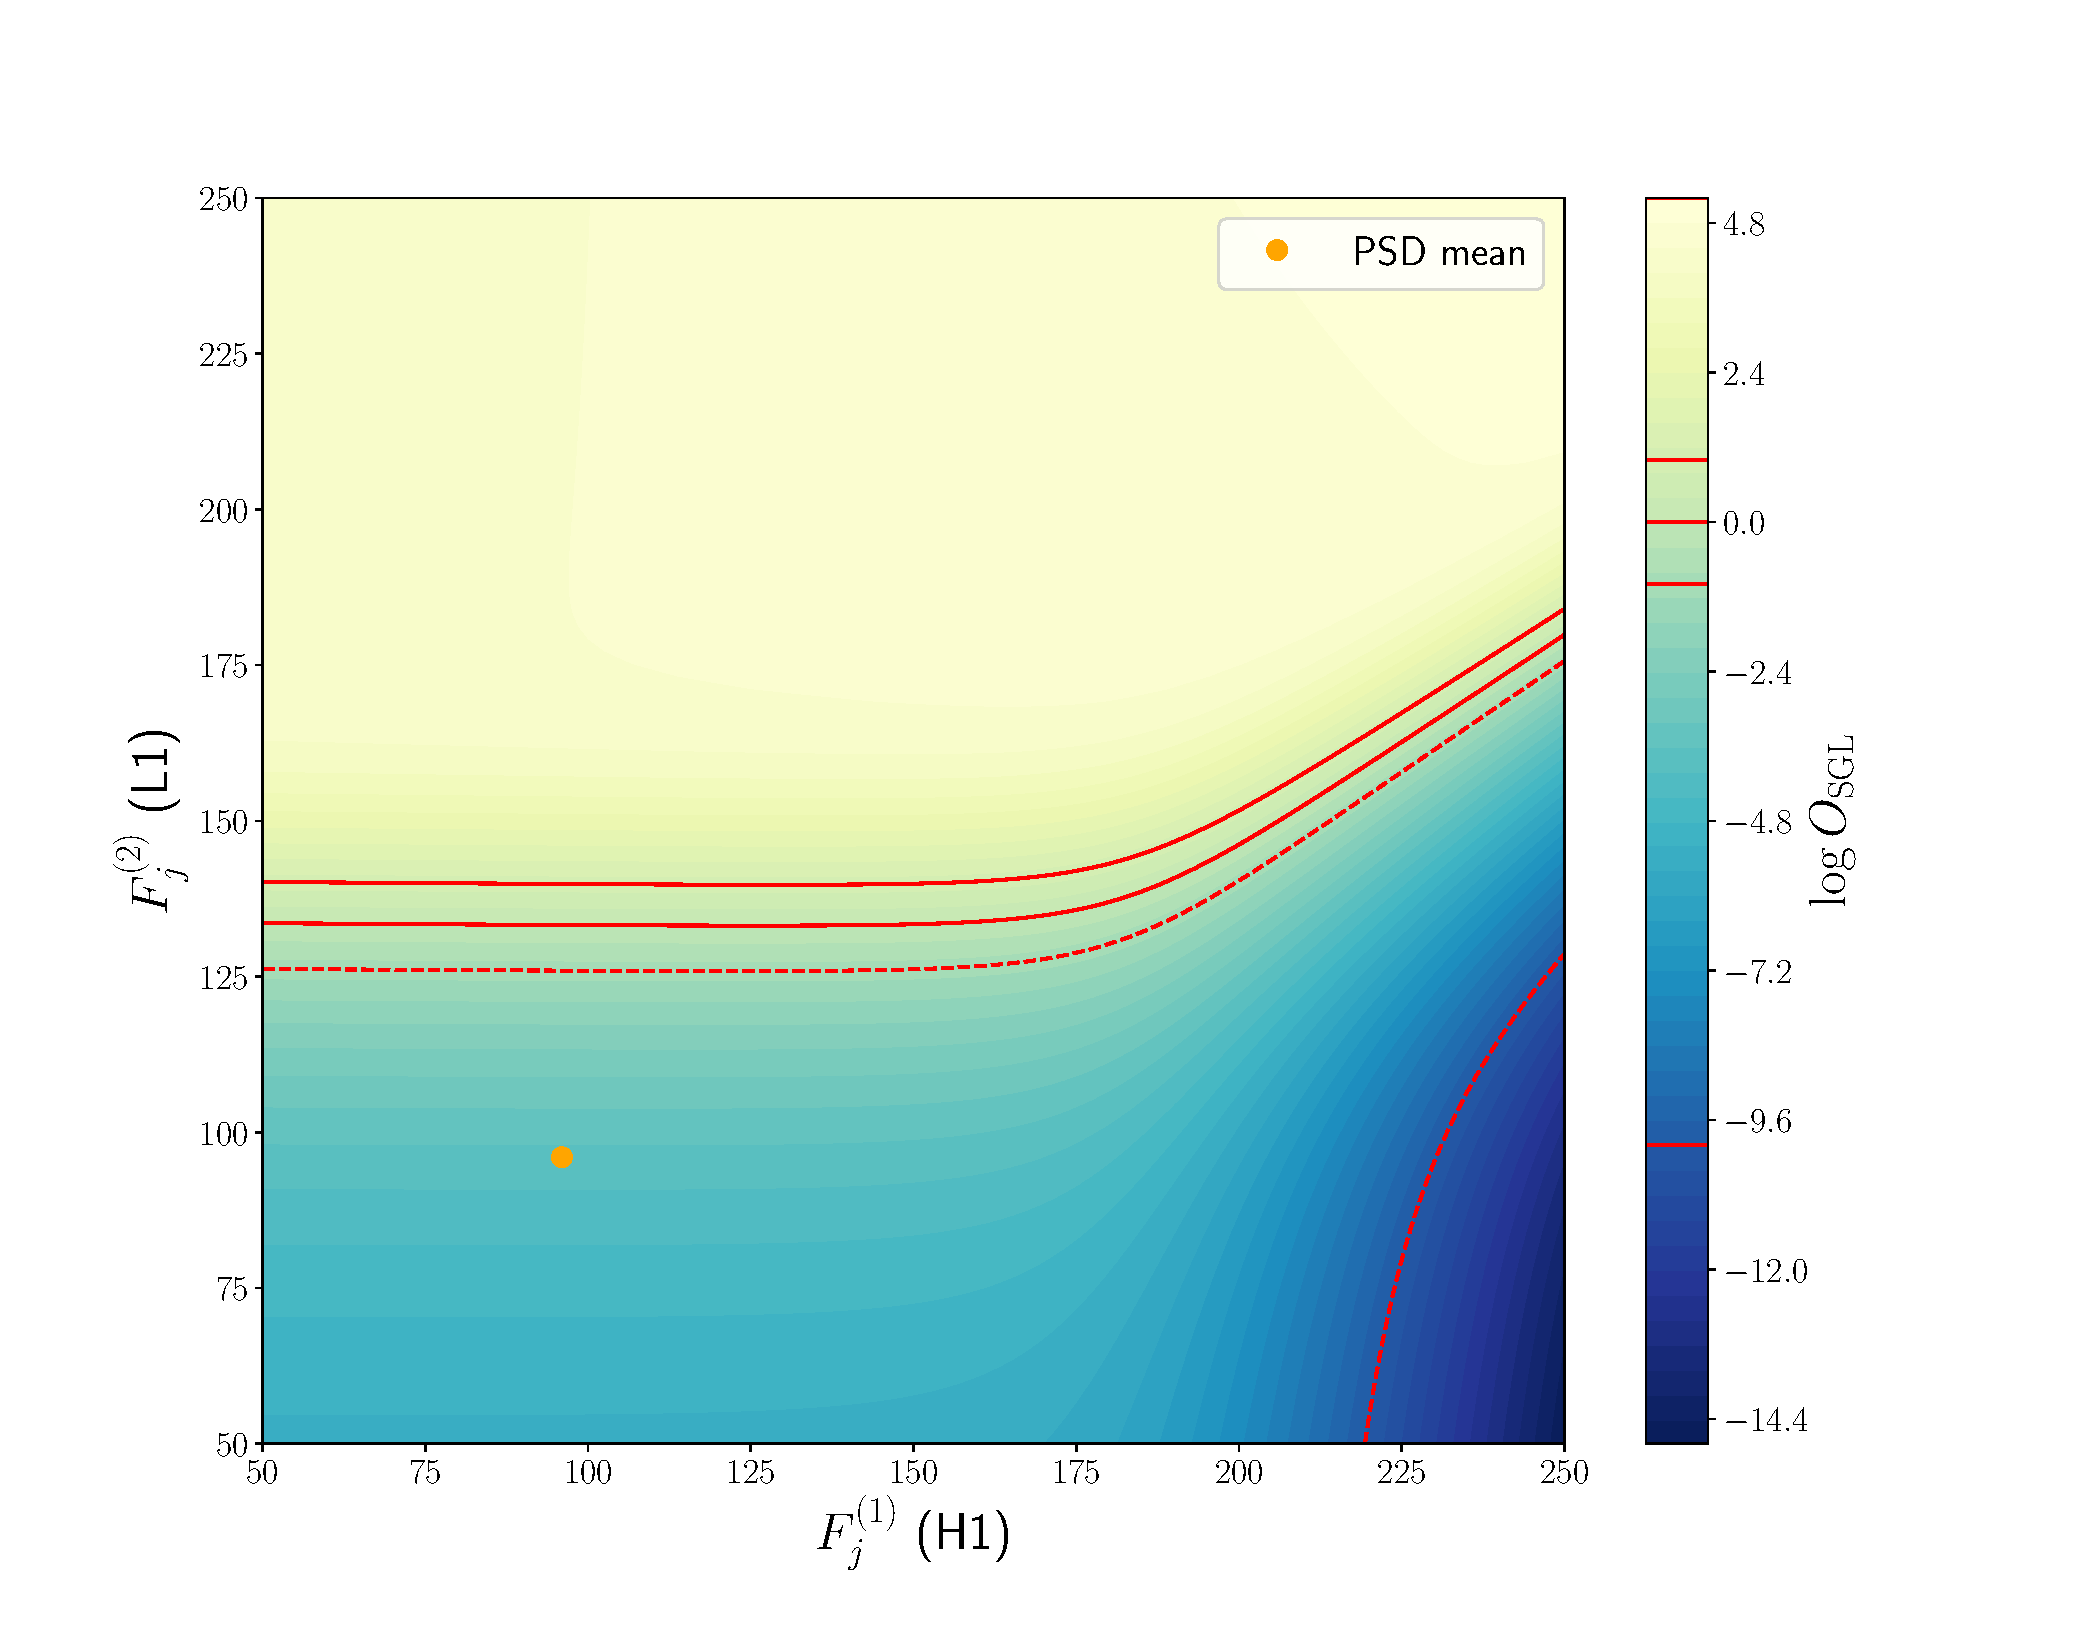
\includegraphics[width=0.9\columnwidth]{C3_soap/lookup_3d_0.pdf}
\end{minipage}\hfill
\begin{minipage}{0.35\linewidth}
\caption{This shows the distribution of the lines aware statistic plotted against the \gls{FFT} power in each detector. This example is for parameters $p_s(\lambda) = 2$,$p_l(\lambda) = 10$ and $p(M_L)/p(M_G) = 1$. Here we expect the \gls{SNR} of a line to be larger than a signal.}
\label{soap:lineawareamp:plot:linebig}
\end{minipage}
\end{subfigure}
\caption[Lookup tables for line aware statistic with consistent amplitude.]{Lookup tables using the line aware statistic for consistent amplitude as in Sec.~\ref{soap:lineawareamp}. Each of these use the parameters $p_s(\lambda) = 4$,$p_l(\lambda) = 5$ and $p(M_L)/p(M_G) = 0.03$. }
\label{soap:lineawareamp:example}
\end{figure}

\section{\label{soap:results} Testing the algorithm}
%%%%%%%%%%%%%%%%%%%%%%%%%%%%%%%%%%%%%%%%%%%%%%%%%%%%%
%
% Introduction to what we are testing on
%
The sensitivity of the algorithm was tested by searching for artificial
signals from isolated pulsars added to three types of noise-like data:
continuous Gaussian noise, Gaussian noise but with periods of missing data,
and real detector data (the S6 \gls{MDC}~\citep{walsh2016ComparisonMethods}). The S6 \gls{MDC} refers to a standardised set of simulated signals which are injected into real data, this set is also what is used for the injections into the two Gaussian noise cases. We describe each
of the tests in more detail in Sec.~\ref{soap:results:gaplessgauss},\ref{soap:results:gausss6} and
\ref{soap:results:s6}, but several common pre-processing steps are performed
before running these datasets through the Viterbi algorithm:
%
% Steps of the viterbi search
%
\begin{enumerate}
%
\item We read \glspl{SFT} generated from 1800\,s stretches of data in 2\,Hz
    bands between 100 and 200\,Hz. The \glspl{SFT} length is chosen to ensure that any signal is likely to be contained within the width of a single
    frequency bin during the length of one day, rather than being split
    across the bin edges (see below).
%
\item We estimate the noise \gls{PSD} for each \gls{SFT} by calculating a
    running median over frequency using LALSuite
    code {\tt XLALSFTtoRnmed} \citep{ligoscientificcollaboration2018LIGOAlgorithm}, this includes a bias factor to
    convert this to the mean and has a width of 100 bins. We then normalise the \gls{SFT} by dividing it
    by its running median, giving the noise-like parts of the spectrum a
    mean power of approximately one.

\item The \glspl{SFT} are then summed over one day, as described in
    Sec.~\ref{soap:sumdata}. The signal parameters are chosen so that
    within the frequencies of the search, the signal will not fall in more than two frequency bins over this
    period.

    The differential Doppler shift of a signal seen at two detector sites due to the Earth's rotation $\Delta f^{(1,2)}_{\rm{rot}}$ is simply
%
\begin{equation} \label{soap:results:doppler}
\Delta f^{(1,2)}_{\rm{rot}} = \frac{({{\bm v}^{(1)}} -{{\bm v}^{(2)}})\cdot
\hat{\bm s}}{c} f_0,
\end{equation}
%
where ${\bm v}^{(1,2)}$ is the velocity of detector $1,2$ in an inertial reference frame, $f_0$ is the
instantaneous signal frequency in the frame, $\hat{\bm s}$ is the unit vector in the direction of the source and  $c$ is the speed of light.
The maximum difference in frequency seen by the two \gls{LIGO} detectors
is 
\begin{equation} \label{soap:results:doppler:diff}
\Delta f_{\rm rot} \approx 6.5\times 10^{-7} f_0,
\end{equation}
%
so the frequency measured from a source in the equatorial plane with $f_0=200$\,Hz will differ by up to $1.3 \times 10^{-4}$\,Hz in the two detectors.
This is $\sim 4$ times smaller than the frequency bin width of 1800\,s \glspl{SFT} ($5.6 \times
10^{-4}$\,Hz), so signals at frequencies lower than this are likely to appear in the same frequency bin in the two detectors. Therefore, whilst at higher frequencies we still allow the signal to be in different frequency bins between the detectors, in the following searches, we do not allow this.
%

\item The data is then split into 0.1\,Hz sub-bands which are overlapping by 0.05\,Hz. These were chosen to ensure that signals are contained within a sub-band over the year. On these timescales the important contributions to the frequency evolution are the spin-down rate of the pulsar and the Doppler shift due to the earth orbit.
To investigate the doppler shift, we can look at a signal at 200\,Hz, using Eq.~\ref{soap:results:doppler} we can calculate the maximum shift in frequency due to the earths orbit as,
%
\begin{equation}
\label{soap:results:dforbit}
\Delta f_{\rm orbit} = \frac{2 \pi R_o}{T_o} \frac{1}{c} f_0 \approx 9.9 \times 10^{-5} f_0,
\end{equation}
%
where $T_{\text{o}}$ and $R_{\text{o}}$ are the
earth orbit time and radius. This gives a maximum doppler shift of $0.019 \; \rm{Hz}$, this is a $\sim 1/5$ of the width of a sub-band, therefore, is more likely to be totally contained within a sub-band than crossing over the edge.
To account for the cases where the signal frequency crosses over the edge of a sub-band, the sub-bands overlap by 0.05\,Hz so that the majority of the signals should be completely contained within at least one of the sub-bands.
To investigate the spin-down of the pulsar, we look at the length of data, $T=4.05 \times 10^7$\,s and we choose a sub-band width of 0.1\,Hz. For a signal to drift over the width of a whole sub-band we would need f-dot of,
\begin{equation}
\frac{df}{dt} > \left|\frac{-0.1}{4.05 \times 10^7}\right| = 2.4 \times 10^{-9} \rm{Hz/s}.
\end{equation}
The majority of the injections that follow satisfy this condition, signals which are greater than this, and therefore drift over multiple bands, are vetoed from the search.
%
\item The two detector Viterbi algorithm is then run using the line aware
statistic (see Sec.~\ref{soap:las}). There are 4 parameters which we optimise in this search. The transition probabilities, where we have one parameter $\tau$ which is the ratio of the probability
of going straight to the probability of going either up or down. Due to the averaging
procedure, the signals received at each detector are forced to follow a common track which is equal to the `imaginary' detectors track. The other three parameters, $w_S, w_L \; \rm{and} \; p(M_L)/p(M_N)$, are described in Sec.~\ref{soap:las}.
%
\item The algorithm then returns the most probable track though the data, and the value
$\propto$ the log-odds in the final time step, i.e., the
maximum final value, $\max_j(V_{N,j})$, in Eq.~\ref{soap:lineaware:stat}, which is then our detection statistic.

%
\end{enumerate}
%
% Example plot of what soap gives
%
As an example of what the algorithm returns, Fig.~\ref{soap:tracks} shows
the tracks in the two detectors, H1 and L1. This also shows the
log-odds ratio of ending in any
frequency bin, i.e., all the elements in Eq.~\ref{soap:lineaware:stat}.  In this figure, each time segment of the odds ratios have been normalised such that the sum of the odds ratios is 1.



\begin{figure*}
%\centering
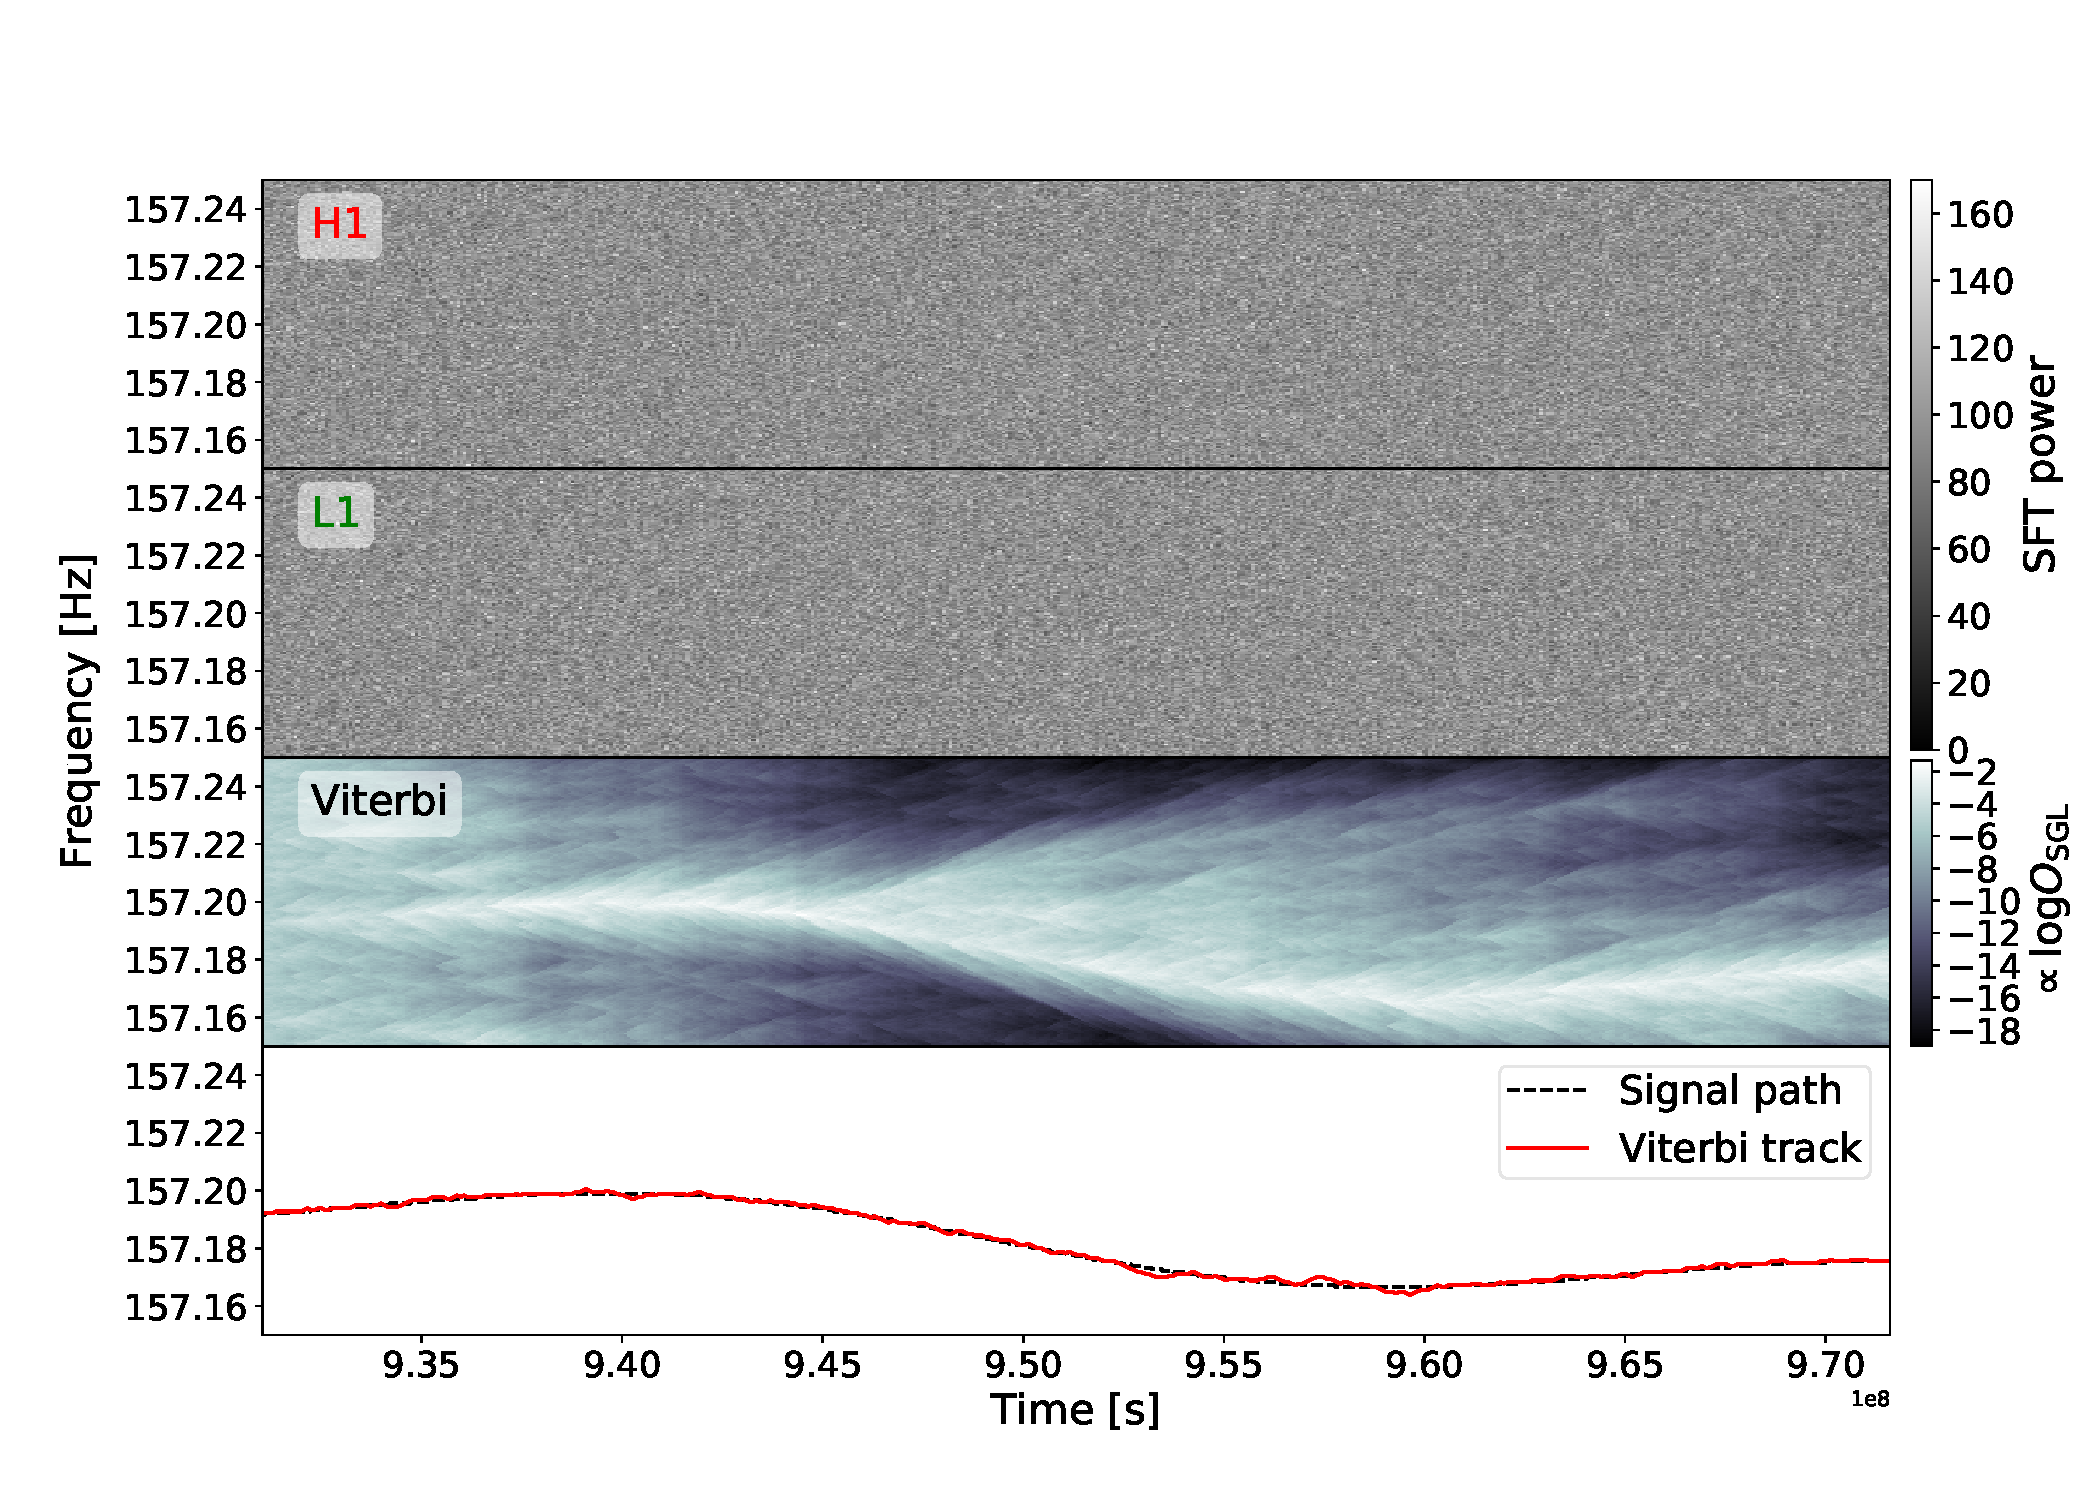
\includegraphics[scale=0.45]{C3_soap/viterbi_tracks.pdf}
%
\caption[Example of SOAP algorithms and outputs when run on H1 and L1 spectrograms.]{\label{soap:tracks} The results that the SOAP algorithm returns from an injection with an optimal
\gls{SNR} of 90, i.e., the \gls{SNR} in H1 is 64 and the \gls{SNR} in L1 is 62.
The signal is injected into Gaussian noise, where the 1800\,s \glspl{SFT} have been
summed over 1 day.  The top panel shows a simulation of summed \glspl{SFT} from H1, the second panel shows the same for L1,
the third panel shows the values proportional to the
log-odds ratios in Eq.~\ref{soap:lineaware:stat}.
The log-odds have been normalised such that the sum of
all the odds ratios in every time bin are equal to 1. The bottom panel shows the injected signal track (black dotted) and the track found in the `imaginary' detector by the two-detector SOAP search with the line-aware statistic (red), both of these tracks are at the geo-centre. In this case the \gls{RMS} of the difference between the Viterbi track and injected signal track was $\sim$1 bin, where 1 bin is 0.00056 Hz wide.}
%
\end{figure*}


In the following tests there are two main quantities which we use to determine
the sensitivity. These are sensitivity depth $\mathcal{D}$ and the optimal
\gls{SNR} $\rho$.  The sensitivity depth, $\mathcal{D}$, is defined in
\citep{behnke2015PostprocessingMethods} as,
%
\begin{equation}
\label{soap:results:sigmoid}
\mathcal{D}(f) = \frac{\sqrt{S_h(f)}}{h_0},
\end{equation}
%
where $S_h(f)$ is the single-sided noise \gls{PSD} and $h_0$ is the \gls{GW} amplitude.  The optimal \gls{SNR} is defined as,
%
\begin{equation}
\rho^2 = \sum_X 4
\Re\int^{\infty}_{0}\frac{\tilde{h}^X(f)\tilde{h}^{X*}(f)}{S^X(f)}df,
\end{equation}
%
 where $X$ indexes the
detectors and $\tilde{h}(f)$ is the Fourier transform of the time
series of the signal $h(t)$. This expression is defined in~\citep{prix2007SearchContinuous} for
a double-sided \gls{PSD} and we have defined it for the more common single-sided
case.

%%%%%%%%%%%%%%%%%%%%%%%%%%%%%%%%%%%%%%%
%%%%%%%%%%%%%%%%%%%%%%%%%%%%%%%%%%%%%
\subsection{\label{soap:results:gaplessgauss}S6 injections into gapless Gaussian noise}
%%%%%%%%%%%%%%%%%%%%%%%%%%%%%%%%%%%%%%%
%%%%%%%%%%%%%%%%%%%%%%%%%%%%%%%%%%%%%%
%
% intro to what data was used and defenitions
%
The first test involves injecting signals into Gaussian noise. The power spectrum of a Gaussian noise time-series follows a $\chi^2$ distribution with two degrees of freedom, therefore, as we search through the power spectrum, we generate spectrograms which follow a $\chi^2$ distribution. 
These spectrograms are 0.1\,Hz wide and are set at 0.05\,Hz intervals between 100\,Hz and 200\,Hz. The bins are $1./1800$\,Hz wide and 1800s long, where the total length of data is the same as S6, i.e., $\sim 1.3$ years.
We then generate the signals, where the pulsars parameters are
fixed to the same values as the injections in the S6 \gls{MDC} in this band, 
these values are outlined in \citep{walsh2016ComparisonMethods}.

%
% describe the pre-pruning of signals
%
The values of $f_0$ for the injections were not always centred in a
sub-band, therefore a number of sub-bands contained only part of the injected
signal. These sub-bands were ignored as they contaminated the signal statistics
and only the sub-band which contained the whole signal was accepted.  This
reduced the number of sub-bands from 2000 to 1762 with the removal of 238
sub-bands containing only part of a signal.
This set also includes signals that
drift across multiple sub-bands due to their high spin-down
rate. Only two signals were removed due to their spin-down values, which were $> 5 \times 10^{-9}$\,Hz/s, these were the two hardware injections in the 100-200\,Hz band.

%
% how roc curves and efficiencies are generated/found
%
For each injection the SOAP algorithm returns the detection statistic described in Sec.~\ref{soap:las} and \ref{soap:results}.
We calculate a false alarm rate, which is the fraction of bands that have no injection that do exceed a given threshold. This is set to 1\% and is used as a detection threshold.
We then take all of the bands and if they pass the threshold we set them as detected, i.e., 1, and if they do not they are set as not detected, i.e., 0.
This then leaves us with a set of binomial data, where the efficiency curves later in the paper are sigmoids which have been fitted to this.
The sigmoid follows,
\begin{equation}
s(x; x_0, k)  = \frac{1}{1-\exp{(-k(x - x_0))}}.
\end{equation}
The fit is done by sampling the posterior, i.e.,
\begin{equation}
\label{soap:results:binomialbayes}
p(x_0, k \mid b) \propto  p(x_0,k)p(x \mid x_0, k),
\end{equation}
where $p(x_0,k)$ is the prior and we set to a flat prior and $p(x \mid x_0, k)$ is the likelihood function which is defined by,
\begin{equation}
\begin{split}
p(\bar{x} \mid x_0, k) = \prod_{j=0}\frac{n!}{k!(n-k)!}s(x_j \mid x_0, k)^{k} \\ (1-s(x_j \mid x_0,k))^{n-k}.
\end{split}
\end{equation}
To plot the efficiency curves and lower and upper error bounds, we sample Eq.~\ref{soap:results:binomialbayes} using \gls{MCMC} and then take the mean and the 5th and 95th percentiles respectively for each point in SNR or depth and plot these.
Fig.~\ref{soap:results:gausss6:eff_snr} and  \ref{soap:results:gausss6:eff_depth} then show the efficiency curves for the analyses plotted against the signals optimal \gls{SNR} and depth respectively.
The parameters of the search and their optimised values are shown in Tab.~\ref{soap:results:parameters}. Where we set the prior on the line model to 0 as this part is irrelevant to this search due to the lack of lines in the data.

%
\begin{table}
\centering
%
\caption[Table of line aware statistic parameters which were optimised.]{Table shows the ranges of the search parameters and their optimised values for injections into  gapless Gaussian noise, Gaussian noise with gaps and the S6 \gls{MDC}. For gapless Gaussian noise and Gaussian noise with gaps, there are 10 parameter values spaced linearly between the limits. For the S6 \gls{MDC} the parameters, $\tau$, $w_{\rm{L}}$ and $w_{\rm{S}}$ were distributed in log space between the limits and $p(M_L)/p(M_N)$ is distributed uniformly. \label{soap:results:parameters}}

%
\bgroup
\def\arraystretch{1.5}
\centering
\begin{tabular}{c c c c c}
\hline
\hline
 & $\tau$ & $w_S$ & $w_L$ & $p(M_L)/p(M_N)$ \\
 \hline
 & \multicolumn{4}{ c }{\textbf{Gapless Gaussian}} \\
\hline
limits & [1.0,1.3]& [0.1,5.0]& None& 0.0\\
\hline
optimised & 1.1 & 2.06 & None & 0.0 \\
 \hline
 & \multicolumn{4}{ c }{\textbf{Gaussian with gaps}} \\
\hline
limits & [1.0,1.3]& [0.1,5.0]& None& 0.0\\
\hline
optimised & 1.1 & 2.06 & None & 0.0 \\
 \hline
 & \multicolumn{4}{ c }{\textbf{S6 MDC}} \\
\hline
limits & [1.0,1.1]& [0.1,5.0]& [0.1,6.0]& [0.0,1.0]\\
\hline
optimised & 1.00000001 & 4.0 & 5.0 & 0.0387 \\
\hline
\end{tabular}
\egroup
\end{table}


%
% 95\% efficiency results and time spent on signal track
%
From this we can determine that in Gaussian noise without gaps, the Viterbi
algorithm can detect to an \gls{SNR} of $\sim60 $ and a depth of $\sim
33$\,Hz$^{-1/2}$ with 95\% efficiency at a 1\% false alarm.

Fig.~\ref{soap:results:gausss6:res_snr} and \ref{soap:results:gausss6:res_depth},
show the \gls{RMS} of the difference between the injected signal track and the track found by Viterbi for \gls{SNR} and sensitivity depth respectively. This shows that at \gls{SNR} of 60, where we are detecting signals with a 95\% efficiency, the signals have a mean \gls{RMS} of $\sim 2$ frequency bins. Here one bin width is 0.00056 Hz therefore, we have and \gls{RMS} of $\sim 0.0012$ Hz. \

%%%%%%%%%%%%%%%%%%%%%%%%%%%%%%%%%%%%%
%%%%%%%%%%%%%%%%%%%%%%%%%%%%%%%%%%%%%
\subsection{\label{soap:results:gausss6} S6 injections into Gaussian noise with gaps}
%%%%%%%%%%%%%%%%%%%%%%%%%%%%%%%%%%%
%%%%%%%%%%%%%%%%%%%%%%%%%%%%%%%%%%%

%
% Intro to what data was used
%
In the second test, we attempt to more closely mirror the S6 \gls{MDC}~\citep{walsh2016ComparisonMethods} in two stages. The first uses the same injection method as Sec.~\ref{soap:results:gaplessgauss} however, removes the \glspl{SFT} where there are gaps in S6. 
The second uses the same injection method again including gaps, however, uses a different value for the noise floor for each \gls{SFT}, this is calculated for each band and \gls{SFT} from S6 data.

Both detectors in S6 had a duty cycle of $\sim$50\%~\citep{aasi2015CharacterizationLIGO}, which means that there are sections of time where there is no data in either one or both detectors. In the sections where one detector is observing but the other is not, the multi detector statistic will not behave correctly as it only has access to data from a single detector.
In these sections we switch from using the multi-detector statistic to the single-detector statistic using the same parameters, these are both defined in defined in Sec.~\ref{soap:las}.

%
% describe the pre-pruning of signals and how efficieny curves were calculated
%
The process of removing sub-bands and generating efficiency curves is the same as in Sec.~\ref{soap:results:gaplessgauss}.


We set a 1\% false alarm rate and generate an efficiency curve for
\gls{SNR} and depth in Fig.~\ref{soap:results:gausss6:eff_snr} and
Fig.~\ref{soap:results:gausss6:eff_depth} respectively. From these efficiency plots we can
see to an \gls{SNR} of $\sim 72$ or a depth of $\sim 13$\,Hz$^{-1/2}$ at a 95\%
confidence with a false alarm of 1\%.

The parameters of the search which were optimised and their optimised values are shown in Tab.~\ref{soap:results:parameters}.


In Fig.~\ref{soap:results:gausss6:res_snr} and ~\ref{soap:results:gausss6:res_depth} show the \gls{RMS} of the difference between the injected signal track and the track found by Viterbi for \gls{SNR} and sensitivity depth respectively. This shows that at \gls{SNR} of 72, where we are detecting signals with a 95\% efficiency, the signals have a mean \gls{RMS} of $\sim 10$ frequency bins (0.0056 Hz).

\begin{figure*}[p]
\centering
\begin{subfigure}[h]{0.49\columnwidth}
\centering
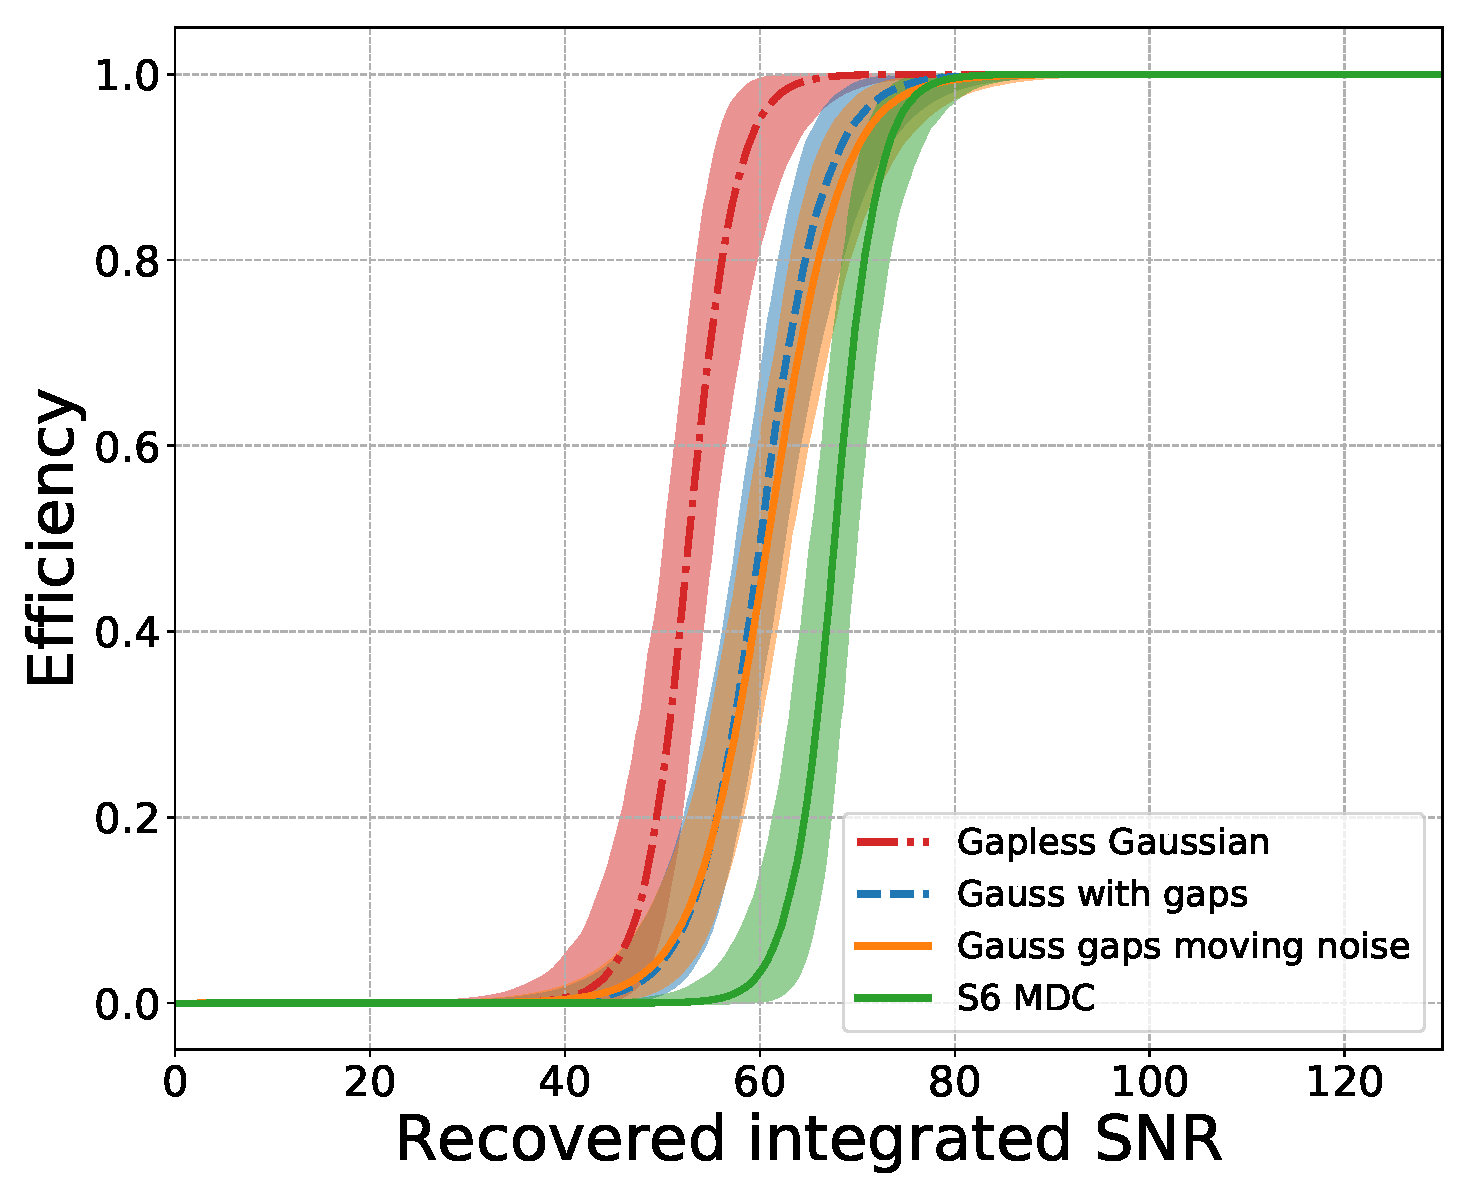
\includegraphics[scale=0.3]{C3_soap/s6_efficiency_snr.pdf}
\subcaption{}
\label{soap:results:gausss6:eff_snr}
\end{subfigure}
\begin{subfigure}[h]{0.49\columnwidth}
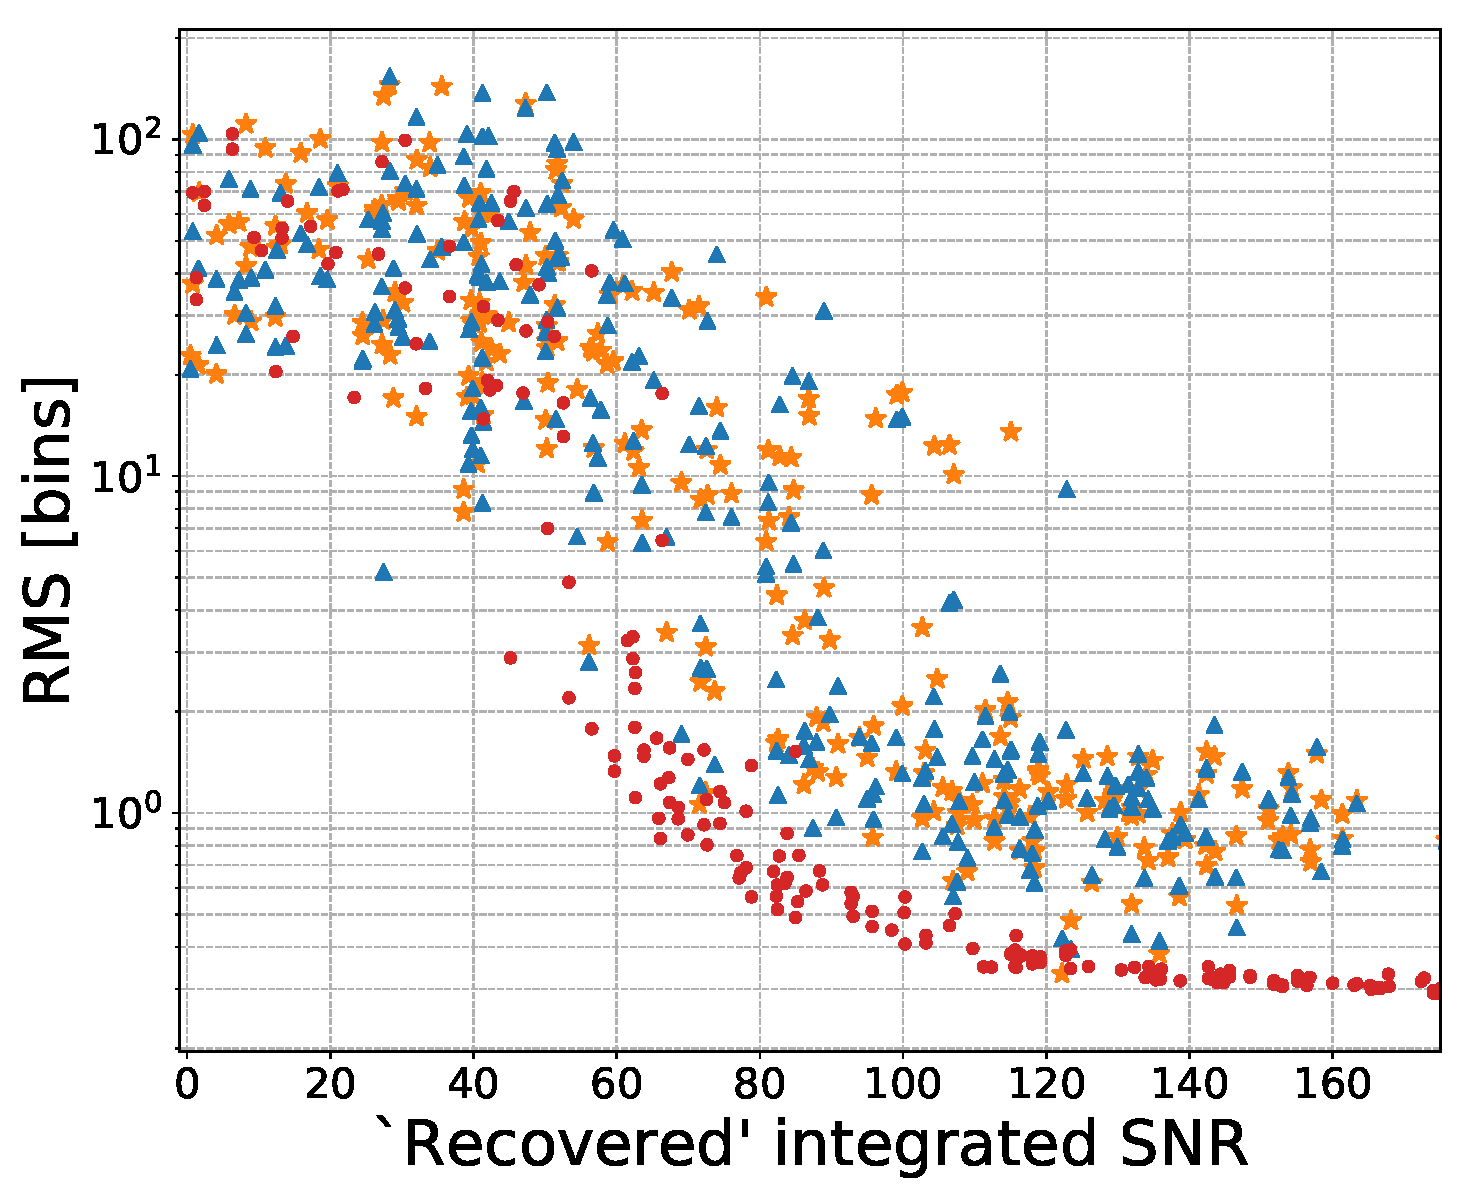
\includegraphics[scale=0.3]{C3_soap/gauss_s6_frac_snr.pdf}
\subcaption{}
\label{soap:results:gausss6:res_snr}
\end{subfigure}

\begin{subfigure}[h]{0.49\columnwidth}
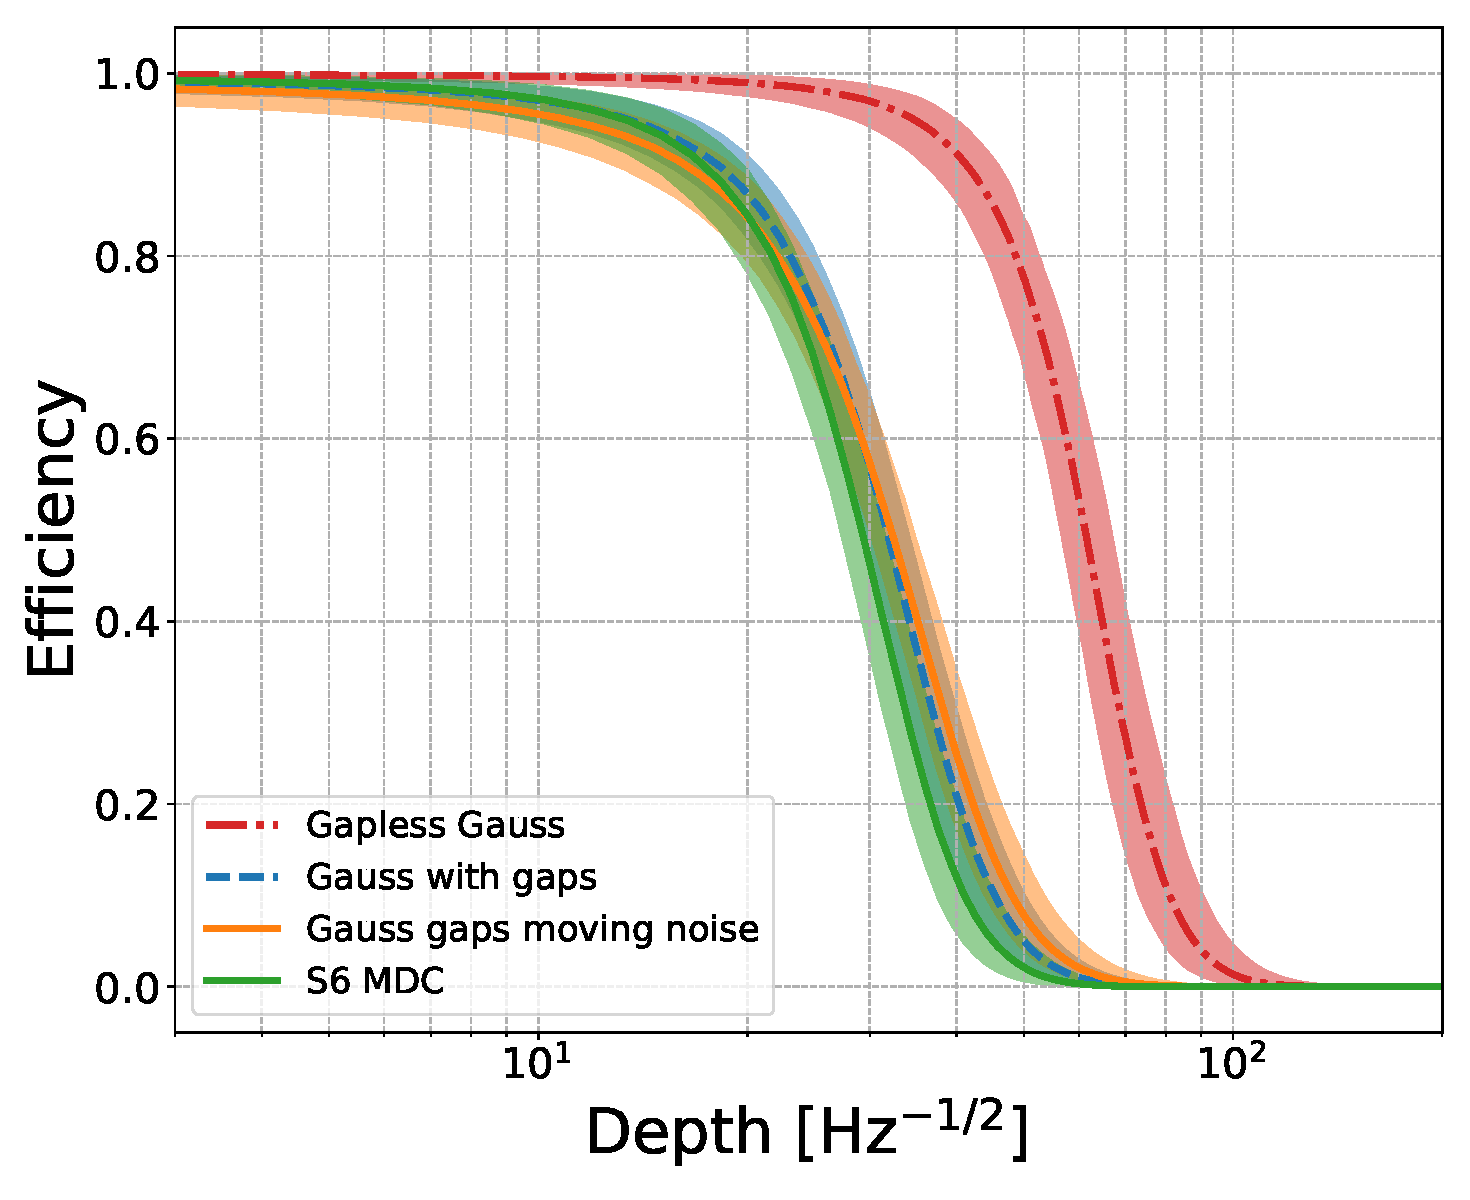
\includegraphics[scale=0.3]{C3_soap/s6_efficiency_depth.pdf}
\subcaption{}
\label{soap:results:gausss6:eff_depth}
\end{subfigure}
\begin{subfigure}[h]{0.49\columnwidth}
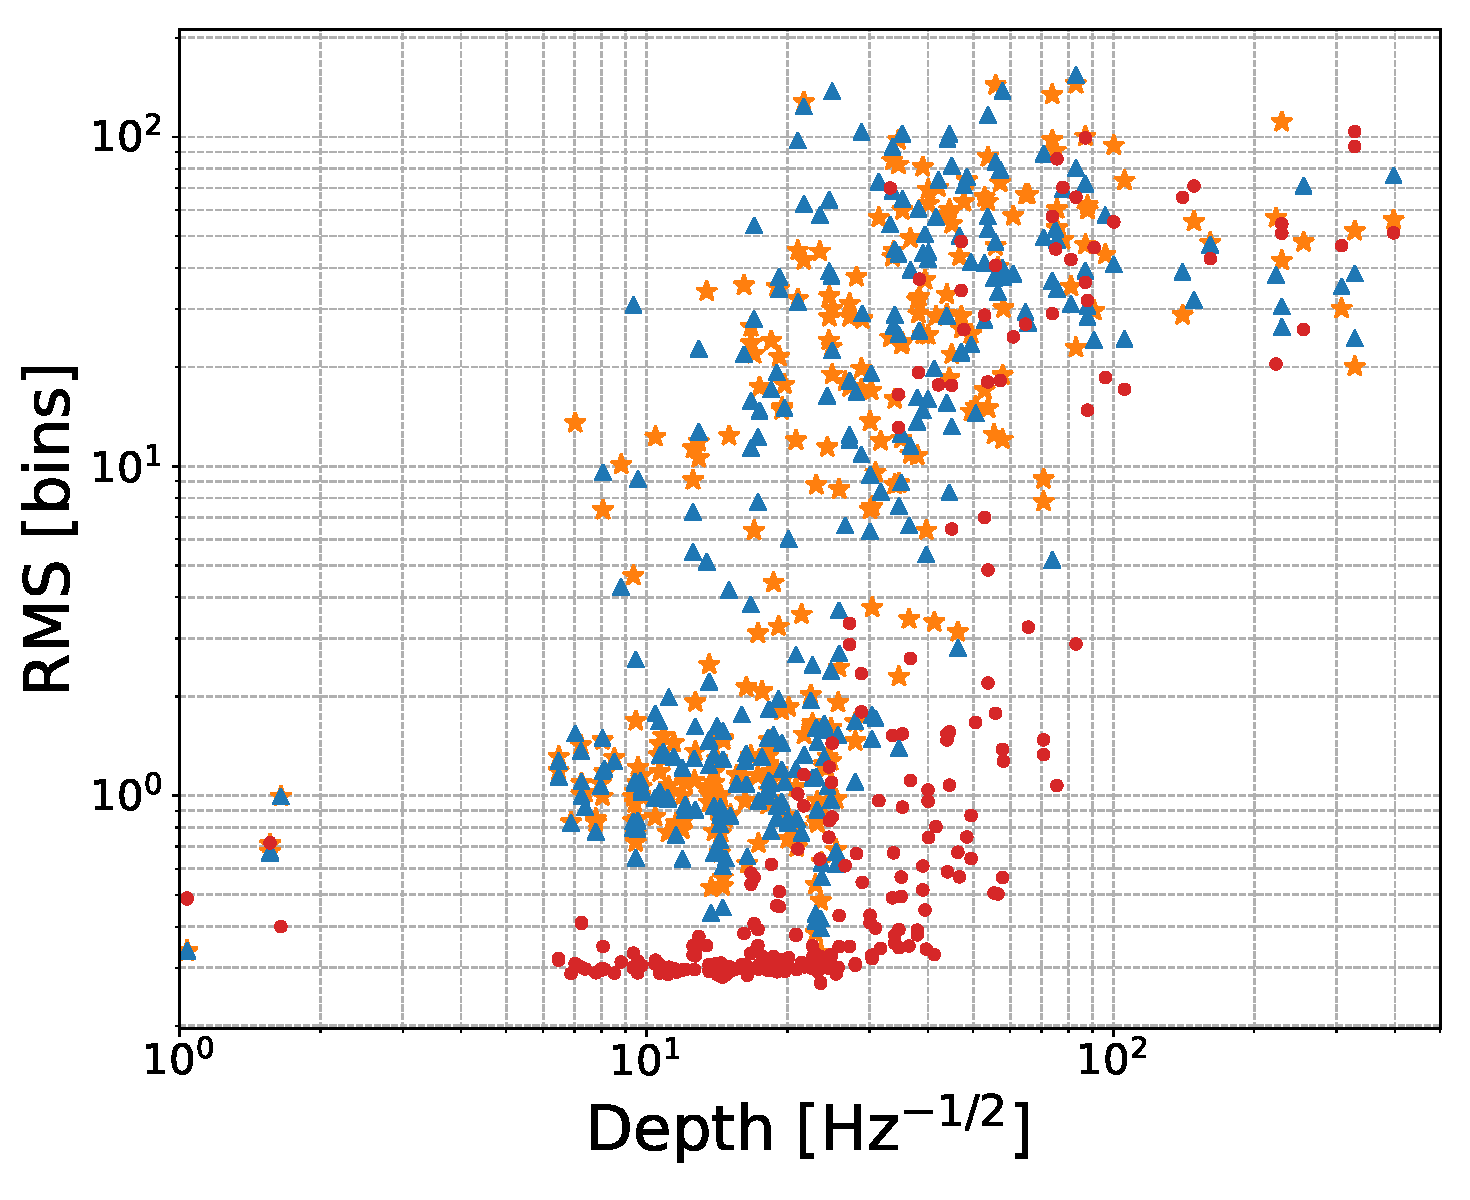
\includegraphics[scale=0.3]{C3_soap/gauss_s6_frac_depth.pdf}
\subcaption{}
\label{soap:results:gausss6:res_depth}
\end{subfigure}

\caption[Sensitivity curves for SOAP search when run on S6 and Gaussian noise.]{Panels \ref{soap:results:gausss6:eff_snr} and \ref{soap:results:gausss6:eff_depth} show the detection efficiency as a function of \gls{SNR} and depth respectively. Here \gls{SNR} is the the integrated \gls{SNR} which we would expect to recover from the available data. The four curves refer to injections into gapless Gaussian noise (red), Gaussian noise with gaps in data, where the noise floor is either fixed (blue-dashed) or it is moving with time (orange) in the same way as the S6~\gls{MDC} and injections into real data i.e., the S6~\gls{MDC}. In the gapless Gaussian noise case, the recovered integrated \gls{SNR} refers to the \gls{SNR} the injection would have if it had the same amount of data as in the cases with gaps.
The curves are made by fitting a sigmoid Eq.~\ref{soap:results:sigmoid} to binomial detection data with a 1\% false alarm rate, as explained in Sec.~\ref{soap:results:gaplessgauss}, the error bounds are the 5\% and 95\% intervals.
At 95\% efficiency and a 1\% false alarm rate, this shows we can detect to an \gls{SNR}  of $\sim 60$ and a sensitivity depth of $\sim 34$\,Hz$^{-1/2}$ for gapless Gaussian noise and an \gls{SNR}  of $\sim 69$ and $72$ and a sensitivity depth of $\sim 13$\,Hz$^{-1/2}$ and $\sim 10$\,Hz$^{-1/2}$ for the Gaussian with gaps case with fixed noise floor and moving noise floor respectively. For the S6 \gls{MDC} we can detect an \gls{SNR} of $\sim 74$ and a sensitivity depth of $\sim 13$\,Hz$^{-1/2}$. 
 Panels \ref{soap:results:gausss6:res_snr} and \ref{soap:results:gausss6:res_depth} show the \gls{RMS} of the difference between the injected signal track and the track found by SOAP as a function of \gls{SNR} and sensitivity depth respectively. This is shown in units of bins where each bin is 0.00056 Hz wide.\label{soap:results:gausss6:plots} }
\end{figure*}


%%%%%%%%%%%%%%%%%%%%%%%%%%%%%%%%%%%%%%%%%%%%%%%%%%%%%%%%%%%%%%%%%%%%%%%%%%%%%%%%
\subsection{\label{soap:results:s6}Tests on the S6 MDC}
%%%%%%%%%%%%%%%%%%%%%%%%%%%%%%%%%%%%%%%%%%%%%%%%%%%%%%%%%%%%%%%%%%%%%%%%%%%%%%%%
%
% Intro to what data was run on and how it was split
%
For a more direct comparison to other \gls{CW} searches and to see how the
algorithm performs with real data, we test the two detector SOAP algorithm using the S6 \gls{MDC}. We focus this search on the 100-200\,Hz band, there are two main reasons for this, one being that this is \glspl{LIGO} most sensitive band and the other is that for much higher frequencies the signal will drift over larger frequency ranges, therefore, our \gls{SFT} length will have to be changed.
Here the 1800\,s \glspl{SFT} are split as in Sec.~\ref{soap:results}, whereafter normalisation, the data is split into 0.1\,Hz wide sub-bands overlapping by 0.05\,Hz.

The two detector SOAP algorithm using the line-aware statistic in Sec.~\ref{soap:las} is then run on each sub-band under the assumption that the detectors have the same sensitivity.
For this search we have four parameters which we optimise, the ranges and optimised values are shown in Tab.~\ref{soap:results:parameters}.

%
% Process of vetoing lines
%
As in Sec.~\ref{soap:results:gausss6}, only the sub-bands which contained the entire frequency evolution of the signal were selected.
Out of the 2000 sub-bands, 238 were removed due the sub-band only containing part of the signals frequency evolution.
The main difference between the analysis for Gaussian noise and real data is that
the real data is contaminated with instrumental lines. This means that whilst the techniques described in Sec.~\ref{soap:las} reduce the number of contaminated bands with a high statistic value, there are still
instrumental lines which are coincident between the detectors and which could not be removed
with these techniques. Within the data there are large number of lines at integer Hertz, which are seen in coincidence between the two detectors, these are thought to originate from digital electronics \citep{coughlin2010NoiseLine}. Therefore the frequency bins $\pm1$ bin of each integer frequency in
Hertz were removed and filled with the expectation value of the noise. To remove instrumental effects at other frequencies,
the sub-bands which gave values of our
statistic above a chosen threshold were investigated by eye. In this case 344 sub-bands were
investigated, and any which were contaminated were vetoed. 
From these 344 sub-bands, 193 were removed from the analysis. The predominant feature in the bands which were removed were broad spectral features which lasted the whole run. Therefore, out of the 2000 sub-bands which are searched over, a total number of 431 sub-bands were removed.

%
% generating efficiency curves
%
The process to calculate the efficiency curves is the same as
in Sec.~\ref{soap:results:gausss6} and \ref{soap:results:gaplessgauss}.

%
% Describe the results plots
%

Fig.~\ref{soap:results:gausss6:eff_depth} and Fig.~\ref{soap:results:gausss6:eff_snr} show the efficiency curves
for \gls{SNR} and depth respectively.  These show that we can detect and
\gls{SNR} of $\sim 74$ and a sensitivity depth of $\sim 13$\,Hz$^{-1/2}$ with
an efficiency of 95\% at a false alarm of 1\%. These results can then be compared to other searches in the S6 MDC comparison paper~\citep{walsh2016ComparisonMethods}. Whilst we only search in the 100 - 200 Hz range, the closest comparison in \citep{walsh2016ComparisonMethods} is the test in the 40 - 500 Hz range, such as in Fig.~4 in \citep{walsh2016ComparisonMethods}. Here our algorithm sits roughly in the middle of all other searches in terms of sensitivity.

%%%%%%%%%%%%%%%%%%%%%%%%%%%%%%%%%%%%%%%
%%%%%%%%%%%%%%%%%%%%%%%%%%%%%%%%%%%%%%%%%
\section{\label{soap:las:optimisation}Optimisation of Line-aware statistic.}
%%%%%%%%%%%%%%%%%%%%%%%%%%%%%%%%%%%%%%%
%%%%%%%%%%%%%%%%%%%%%%%%%%%%%%%%%%

For the above searches we used optimised versions on the line aware statistic,
however, we have yet to explain how this was optimised.  The aim is to find the
best parameters for any given search; the four parameters are
$\tau$,$p_S(\lambda)$, $p_L(\lambda)$ and $p(M_L)/p(M_G)$~\chris{by the way,
any subscripted quantity that is not a variable but instead stands for an
English word (L or G in your case here) should NOT be in italics.}.  We find
the optimum values empirically by running the entire search for each parameter
value that needs to be tested. This is possible as the search is relatively
fast, this will be explained in Sec~.\ref{soap:results:time}.  The line aware
statistic is time consuming to calculate, therefore, to reduce the
computational time, it is pre-calculated and placed into lookup tables such
that it is calculated once and called many times.  These lookup tables were
calculated for values of \gls{FFT} power $F$~\chris{have you always called it
F?} in the range 1 to 400 in each of
the detectors as shown in Fig.~\ref{soap:las:osgl_plots}. For each parameter
the ranges in which they were optimised were chosen based on expected
\glspl{SNR} of each of the injections~\chris{grammar and a bit vague}. 

We can then use a measure of the sensitivity of that search and pick the lookup
table~\chris{not the table. You pick the set of optimal parameters that
generated the table} which gives the highest sensitivity. 
We measure the sensitivity by taking the value of \gls{SNR} which is at 80\% efficiency at 1\% false alarm. 

\subsection{Gaussian noise simulations}

For injections into Gaussian noise, we know that there are no instrumental
lines, therefore, we do not need to optimise over the `lines' part of the
statistic and can set the parameter $p(M_L)/p(M_G)$ to zero which renders the
parameter $p_L(\lambda)$ redundant. 
This then reduces the complexity of the problem by leaving us with only two parameters to optimise over, $\tau$ and $p_S(\lambda)$. 
Whilst this optimisation was partially done in Sec.~\ref{soap:results}, with the result in Tab.~\ref{soap:results:parameters}, this is repeated more completely here.
The parameters were optimised in the range shown in Tab.~\ref{soap:las:optimisation:table}. 

%
\begin{table}
	\centering
	%
	\caption[Table of optimisation parameters for line aware statistic.]{Table shows the ranges of the search parameters and their optimised values for injections into Gaussian noise and the S6 \gls{MDC}. For Gaussian noise there are 30 parameter values spaced linearly between the limits. For the S6 \gls{MDC} the transition matrix parameters, $\tau$, had three values space between the limits. This is because the search is relatively insensitive to this parameter. The parameters $w_{\rm{L}}$, $w_{\rm{S}}$ and $p(M_L)/p(M_N)$ had 10 parameters distributed in linearly between the limits. \label{soap:las:optimisation:table}}
	
	%
	\bgroup
	\def\arraystretch{1.5}
	\centering
	\begin{tabular}{c c c c c}
		\hline
		\hline
		& $\tau$ & $w_S$ & $w_L$ & $p(M_L)/p(M_N)$ \\
		\hline
		& \multicolumn{4}{ c }{\textbf{Gaussian noise}} \\
		\hline
		limits & [1.0,1.1]& [0.1,7.0]& None& 0.0\\
		\hline
		& \multicolumn{4}{ c }{\textbf{S6 MDC}} \\
		\hline
		limits & [1.0,1.1]& [0.1,10.0]& [0.1,20.0]& [0.0,0.3]\\
		\hline
	\end{tabular}
	\egroup
\end{table}

For each point in Fig.~\ref{soap:las:optimisation:gauss}, the entire SOAP search was run using the corresponding parameters as input. 
Efficiency curves are then generated for each of these runs and the values for the \gls{SNR} at 80\% efficiency are recorded. 
Fig.~\ref{soap:las:optimisation:gauss} then shows the 80\% efficiency for each parameter value.
There appears not to be any single value which gives an optimum, however, the dark stripe in Fig.~\ref{soap:las:optimisation:gauss} running from the bottom left to the red cross is the combinations of parameters which give the best result. 
The point where the red lines cross is the parameters used in previous searched in Sec.~\ref{soap:results:gaplessgauss} and \ref{soap:results:gausss6}.
This falls on the line where the algorithm performs best. 
Venturing far from this `optimum' line does not change the results a great deal as the \gls{SNR} does not change much.
The search is then not particularly sensitive to choice of parameters in Gaussian noise.

\begin{figure}[h]
    \centering
    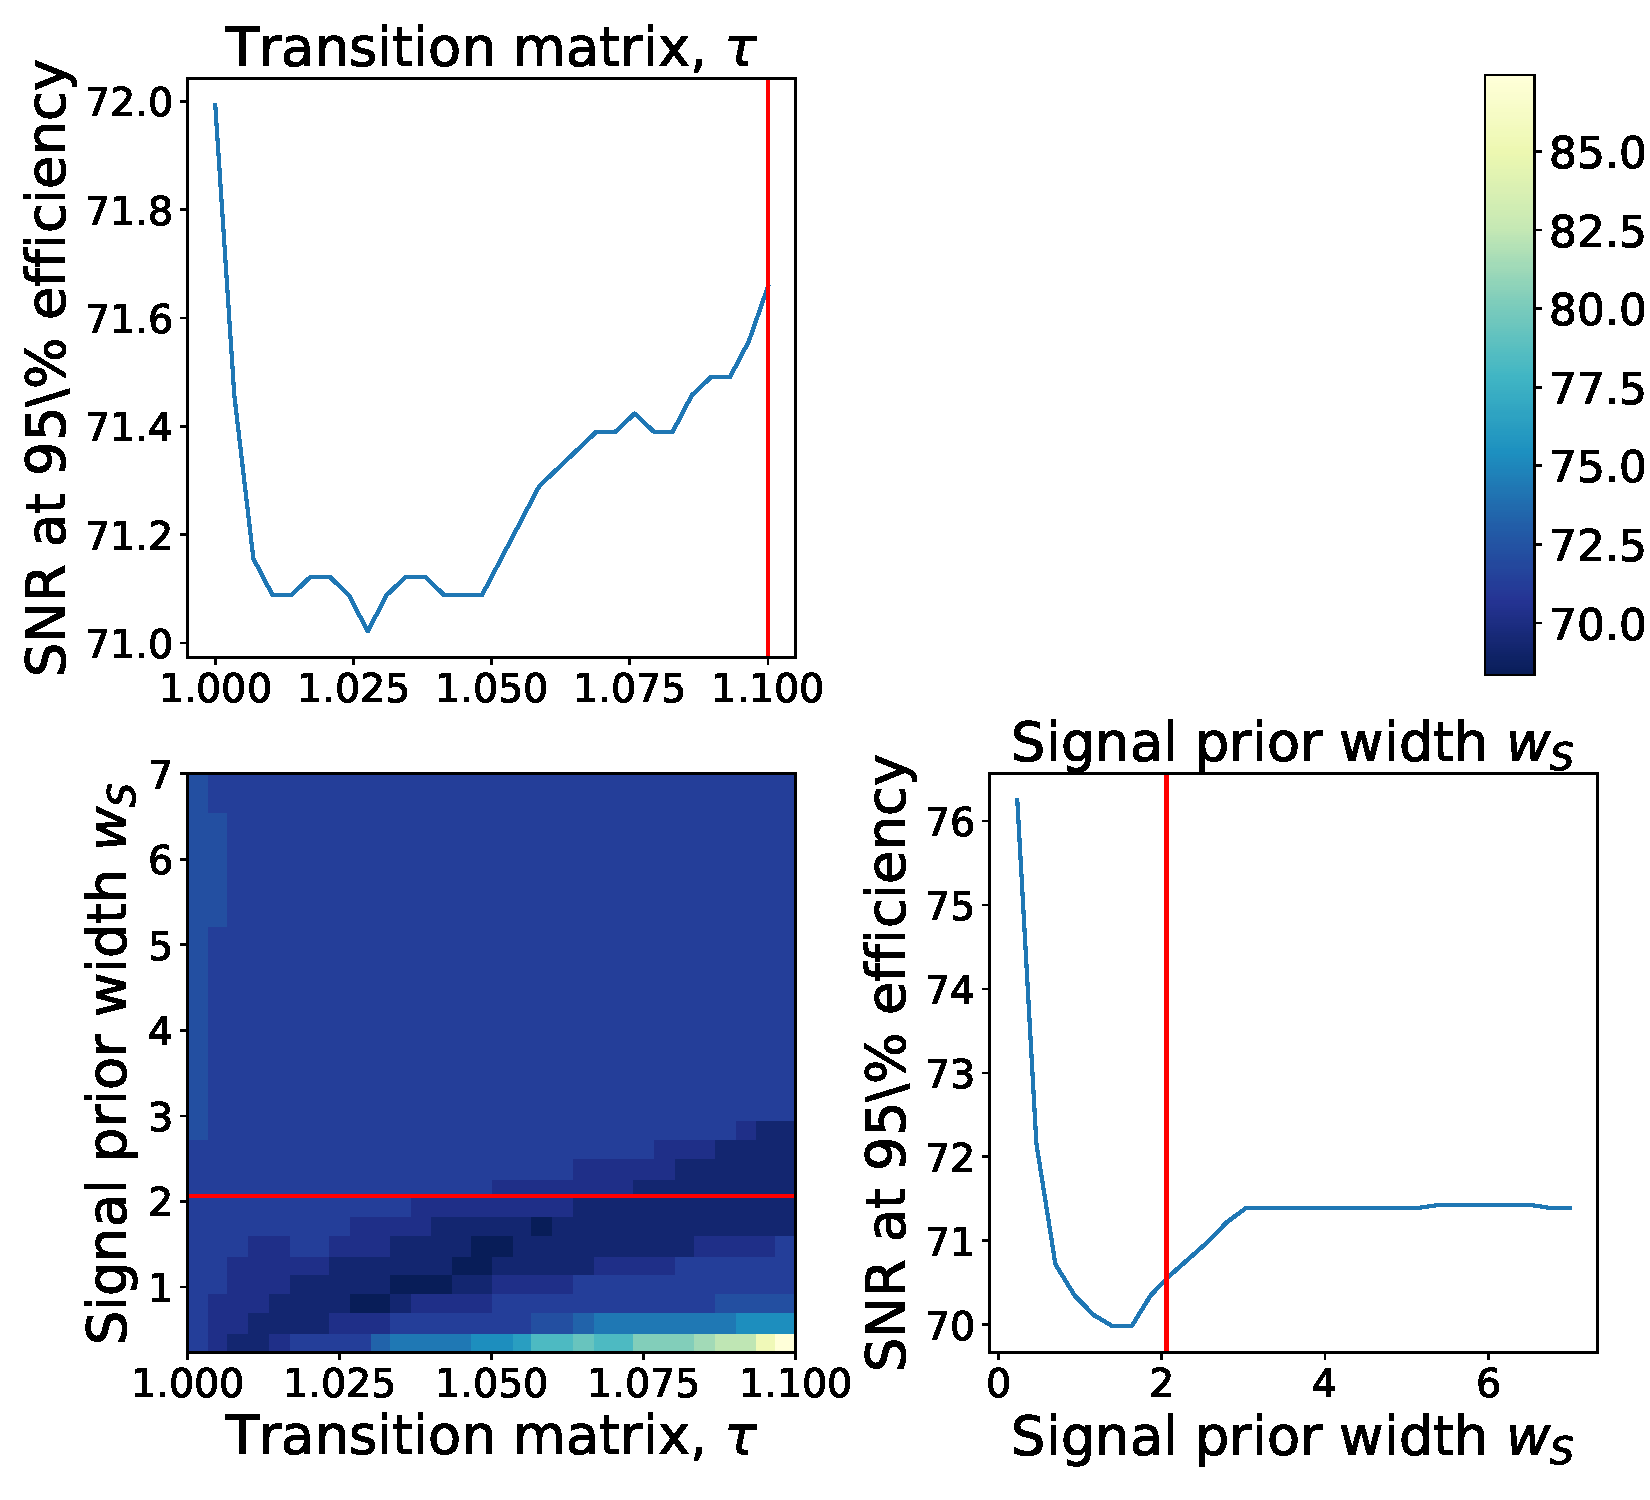
\includegraphics[width=0.9\linewidth]{C3_soap/gauss_optimised.pdf}
    \caption[Optimisation of line aware statistic in Gaussian noise.]{In Gaussian noise the transition matrix parameter $\tau$ and the width of the prior on the signal case $w_S$ were optimised. The key part to remember when reading this plot is that the lower the value of \gls{SNR} the better the search has performed. Therefore darker blue areas are when the search performed better. This map shows that there is a line in parameter space where the search performed best. Also in Gaussian noise, the search is not that sensitive to the choice of parameter. The red lines on here shows the parameters used in the searches in this section. }
    \label{soap:las:optimisation:gauss}
\end{figure}


\subsection{S6 MDC injections}

As the S6 \gls{MDC} data-set is real detector data, there are many examples of instrumental lines. 
This is where we expect the line-aware statistic to have the greatest effect in rejecting lines. 
Here the all of~\chris{grammar} the four parameters are optimised over in the ranges described in Tab.~\ref{soap:results:parameters}. 
This greatly increases the number of lookup tables which need to be generated
and therefore the number of times the search needs to be run. 
Fig~.\ref{soap:las:optimisation:s6mdc}~\chris{Never use an abreviated form when
starting a sentence - Fig. Tab. Sec. Eq. etc...} shows the slices through
parameters~\chris{lots of typos like this, be careful} space for each of the parameters where the values are the \glspl{SNR} at 80\% efficiency.  
These slices are made by taking the mean~\chris{if you're taking the mean then
these aren't slices, they're projections or marginalisations. Why are you
taking the mena anyway?} across the parameters not shown in the figure.
The range chosen for the transition matrix parameter $\tau$ as~\chris{typo} small with a small number of points, this is because the impact of this parameter was expected to be small. 
Fig~.\ref{soap:las:optimisation:s6mdc} demonstrates that changing this
parameter does not have much affect~\chris{should be effect} on the final sensitivity. 
The parameter $w_S$ appears to have a clear location around a value of $3$ where the sensitivity is at a minimum. This is not far from the value of the parameter which is used for all other searches in this thesis (the red line).
The parameters $w_L$ and $p(M_L)/p(M_G)$ show that the sensitivity drops substantially as the values increase. 
In these examples the optimum value may be out of the range chosen here.
Whilst this could be improved slightly by running with a larger parameter
space, this is a time consuming process~\chris{boo-hoo. Not a very strong
argument against extending the range}.
The results in Sec.~\ref{soap:results} show that the current values of the parameters (red lines in Fig~.\ref{soap:las:optimisation:s6mdc}) are sufficiently sensitive when compared to other searches.
To choose optimum parameters for this search, the minimum point for each parameter was chosen. 
This is the minimum in each of the diagonal plots in Fig~.\ref{soap:las:optimisation:s6mdc}.
These values are,
\begin{equation}
\begin{split}
	\tau &= 1.0 \\
	w_S &= 3.0 \\
	w_L &= 20.0 \\
	p(M_L)/p(M_G) &= 0.2879 .
\end{split}
\end{equation}
~\chris{We've discussed that the obvious thing to do is to take the global
minimum value. I don't think you are doing this. You are taking the
marginalised values. You do not explain why you do this.}

\begin{figure}[p]
    \centering
    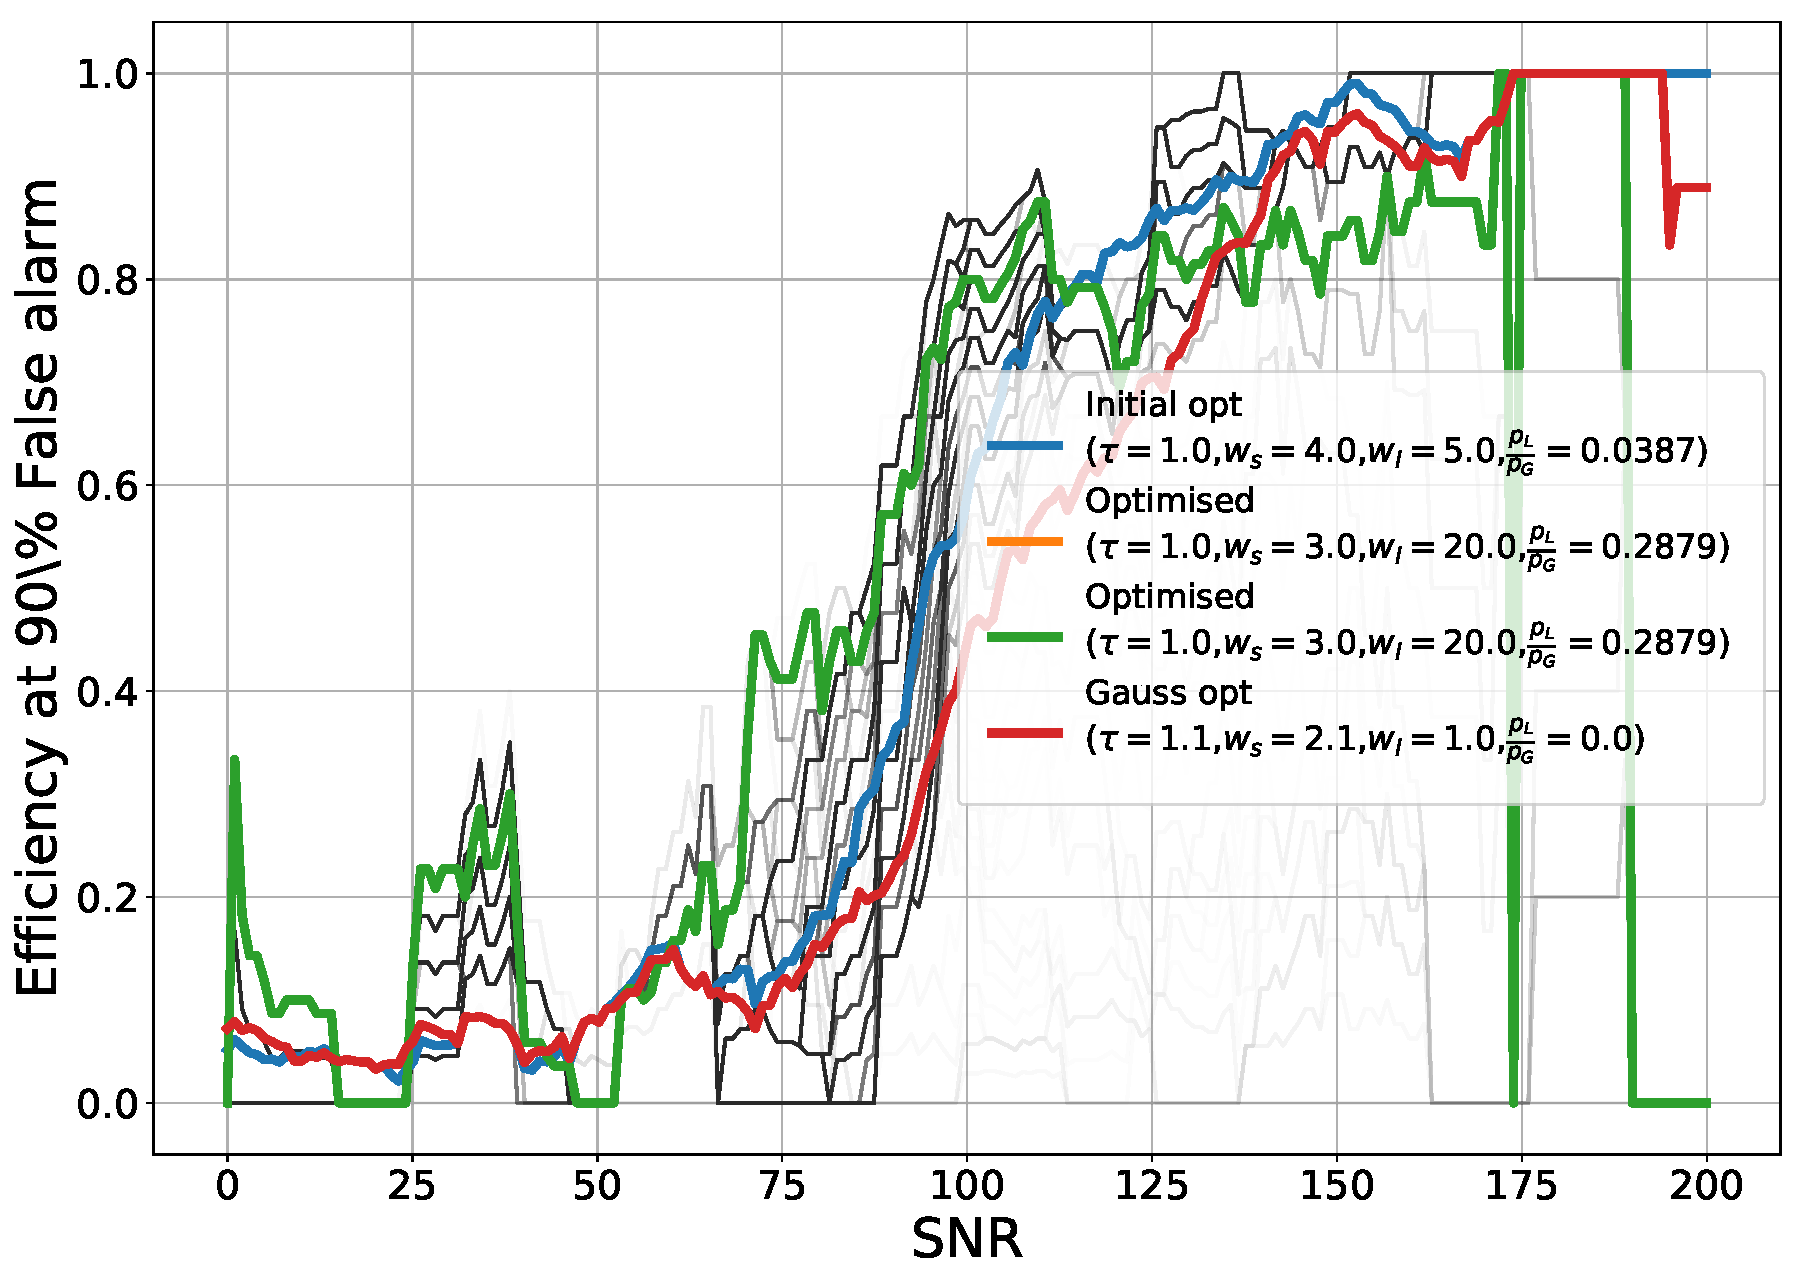
\includegraphics[width=\linewidth]{C3_soap/s6_optimised.pdf}
    \caption[Optimisation of line aware statistic in real S6 data.]{When using real S6 data, all four parameters of the search were optimised over on simulations in real data. The plot above shows the \gls{SNR} at 80\% efficiency for each of the parameters where the ranges are in Tab.~\ref{soap:las:optimisation:table}. Lower values of \gls{SNR} mean the search is performing better. The red lines show the parameters used in the searches in this section and the sections that follow. Whilst this does not seem optimal, the search does not underperform much using the current choice of parameters (red). }
    \label{soap:las:optimisation:s6mdc}
\end{figure}

To visualise how these better optimised parameters are to the values used in
Sec.~\ref{soap:results} we can compare how they perform on a simulated signal
in a time-frequency spectrogram.  In one of the detectors a narrow instrumental
line can also be simulated.  In Fig.~\ref{soap:las:optimisation:vitexample} an
example a \gls{CW} signal injected into Gaussian noise in both
detectors~\chris{2 previous short senetnces seem incomplete and unconnected}.  In
the Gaussian noise optimised case the search is looking for high power in both
detectors which the strong instrumental line satisfied when the astrophysical
signal is weak.  The S6 optimised statistic looks for more consistent \gls{SNR}
in each of the detectors.  The two different lines~\chris{be more specific -
what lines?} show the statistic optimised
on the Gaussian noise injections and the S6 \gls{MDC} injections.  This
demonstrates how the `line aware' statistic improves the robustness of the
algorithm against non astrophysical signals. 

\begin{figure}[h]
    \centering
    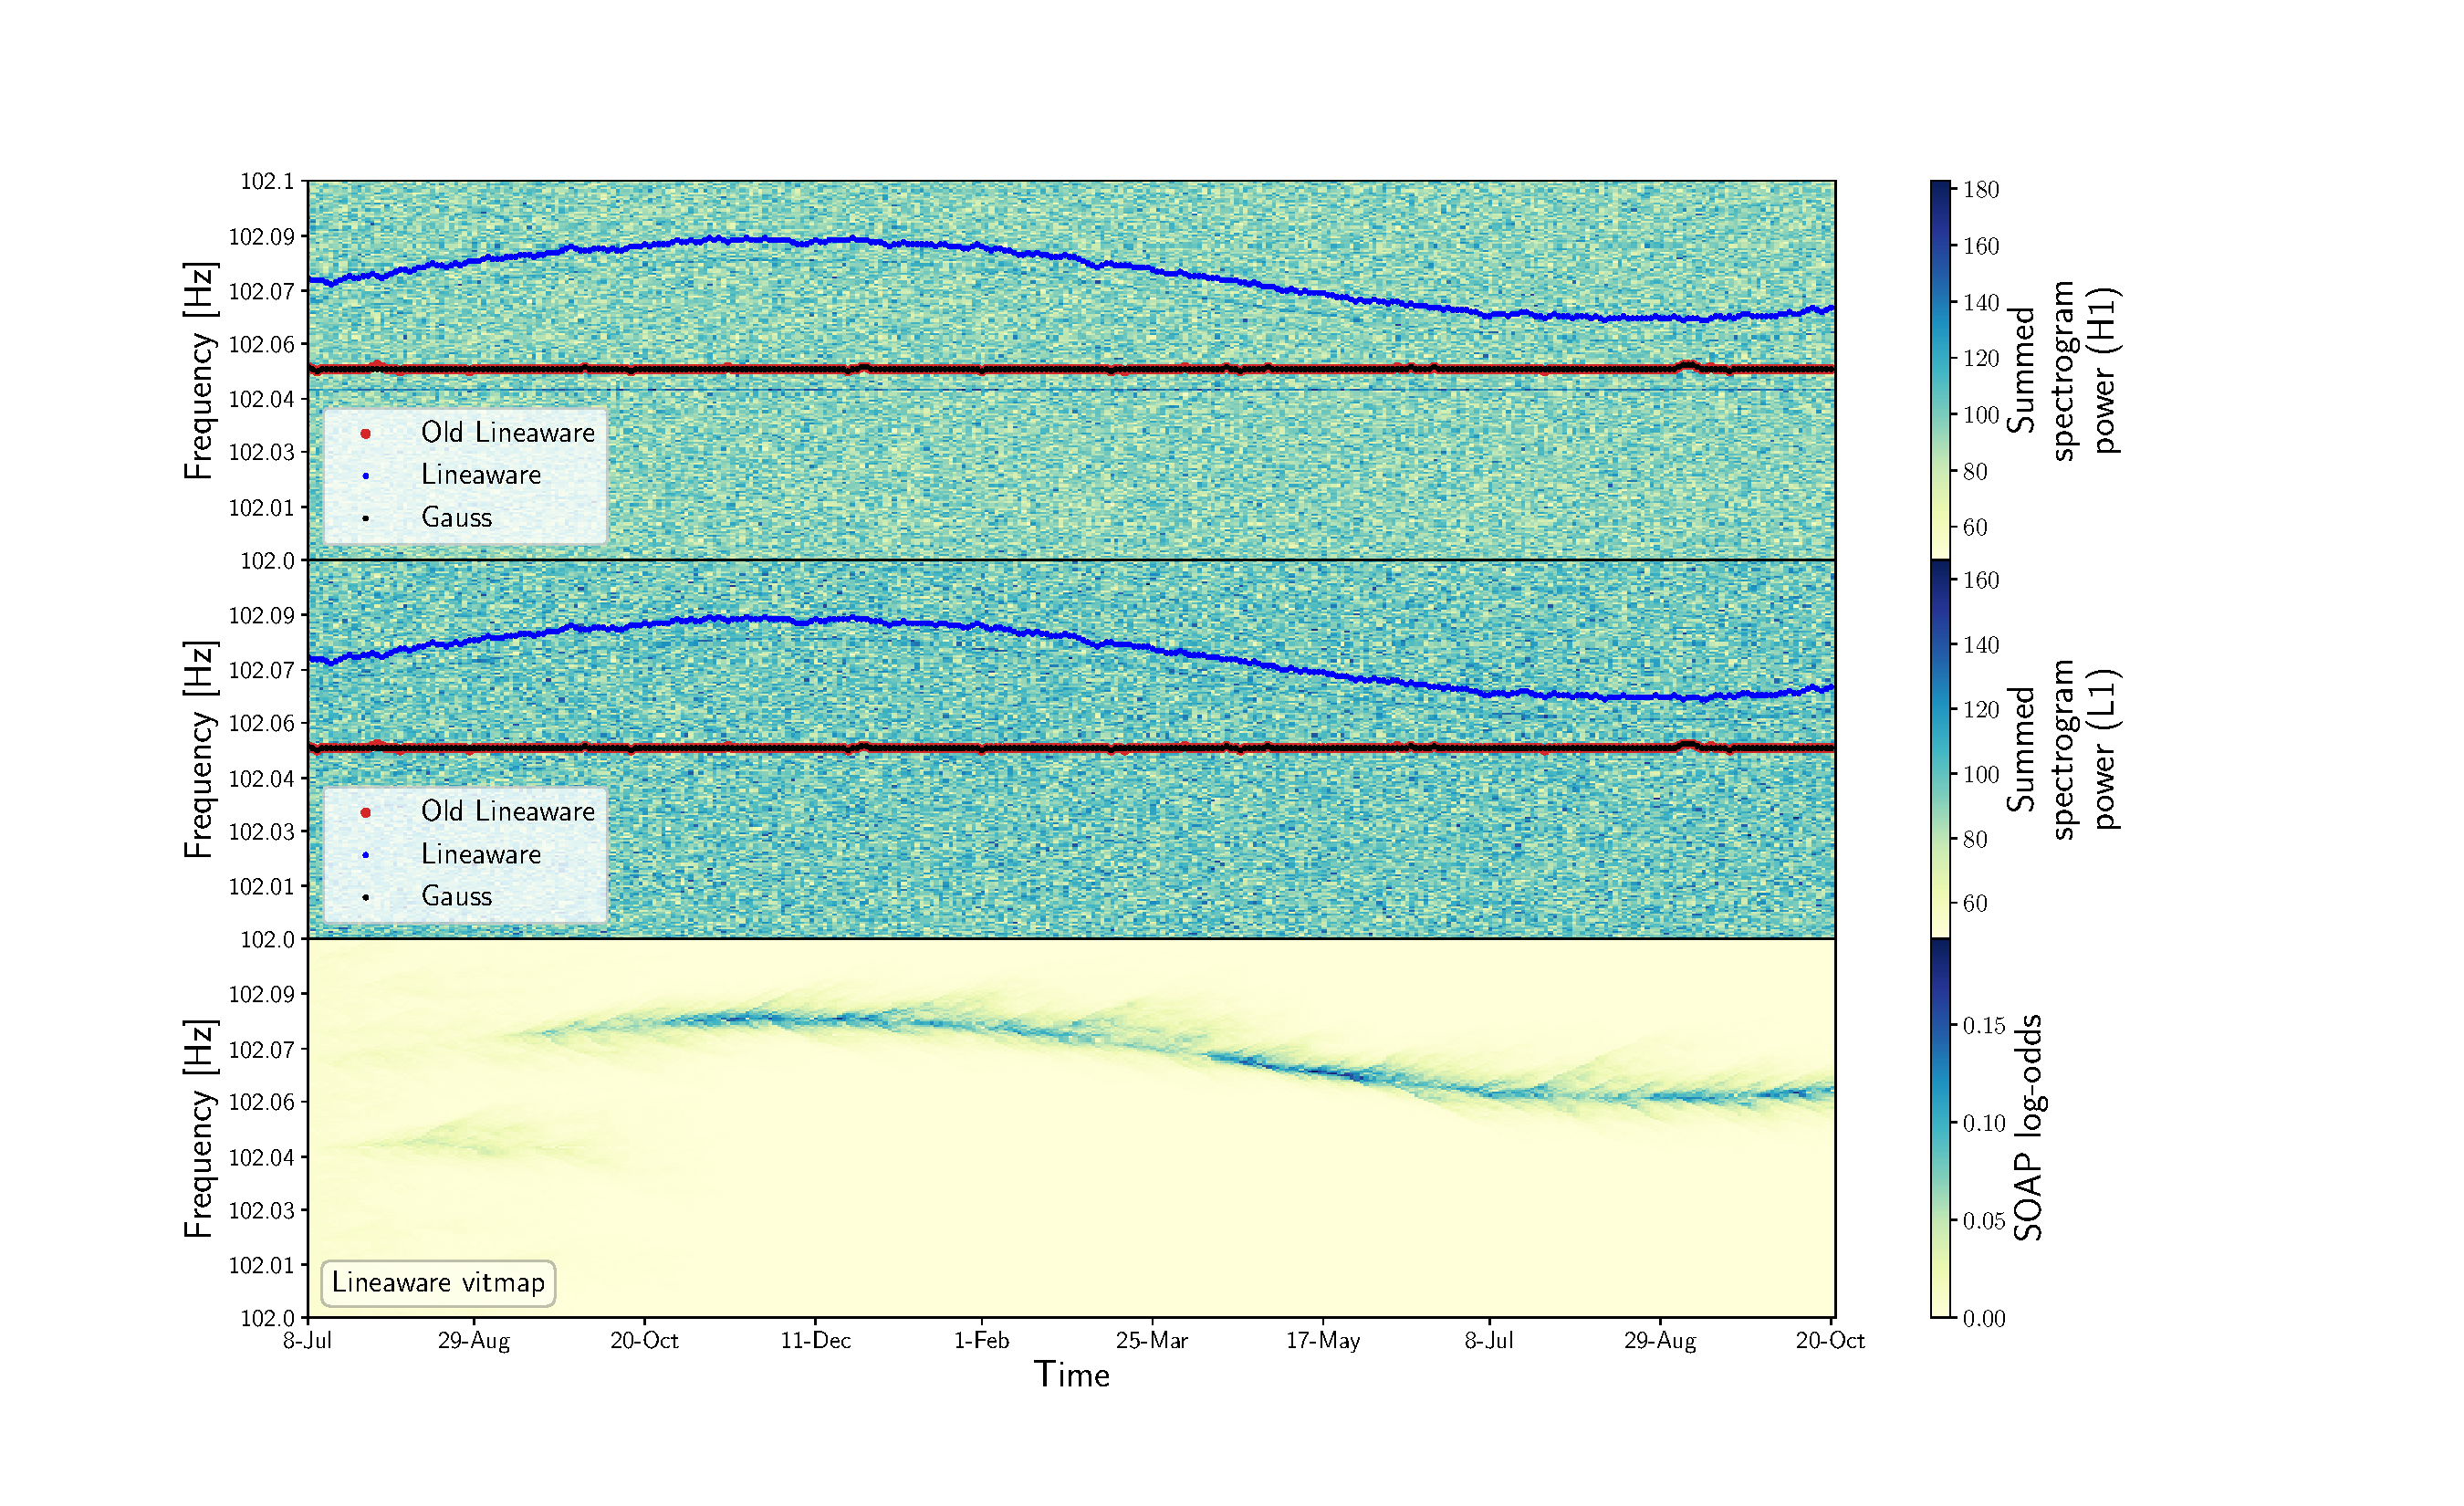
\includegraphics[width=0.9\linewidth]{C3_soap/line_example.pdf}
    \caption[Example of improvements when using optimised parameters for line aware statistic.]{As a visualisation of the line aware statistic working, an astrophysical signal was simulated in both the H1 and L1 detectors. In one detector an instrumental line was added. In the top panel above the tracks identified by different values of the line aware statistic are shown shifted up by 10 frequency bins. This allows the underlying feature to be identified. In the top two panels the sinusoidal nature of the \gls{CW} signal can be identified in the data, and was identified by the line aware statistic using the S6 MDC optimal values (blue line). The top panel also contains a narrow spectral line at $\sim 102.5$ Hz. The values of the statistic optimised for the Gaussian noise case do not identify the signal but identify the spectral line as the most likely signal. The final panel shows the Viterbi map for the statistic values optimised in the S6 MDC. }
    \label{soap:las:optimisation:vitexample}
\end{figure}

\subsubsection{Comparison of sensitivity}

To compare the different parameters of the line aware statistic, three parameter sets were used. 
The optimised values for the Gaussian noise case and the S6 \gls{MDC} case above are used alongside the values optimised in Tab.~\ref{soap:results:parameters}.
These three parameter sets are run on the S6 \gls{MDC} simulations between 40 and 500 Hz to compare their sensitivity. 
The process of running on the S6 \gls{MDC} and generating the efficiency curves is the same as in Sec.~\ref{soap:results}.
Fig.~\ref{soap:las:optimisation:comparison} shows the efficiency curves at a 10\% false alarm rate. 
This, along with Fig.~\ref{soap:las:optimisation:gauss} and \ref{soap:las:optimisation:s6mdc} shows that the search is relatively insensitive to the choice of parameters.

\begin{figure}[h]
	\centering
	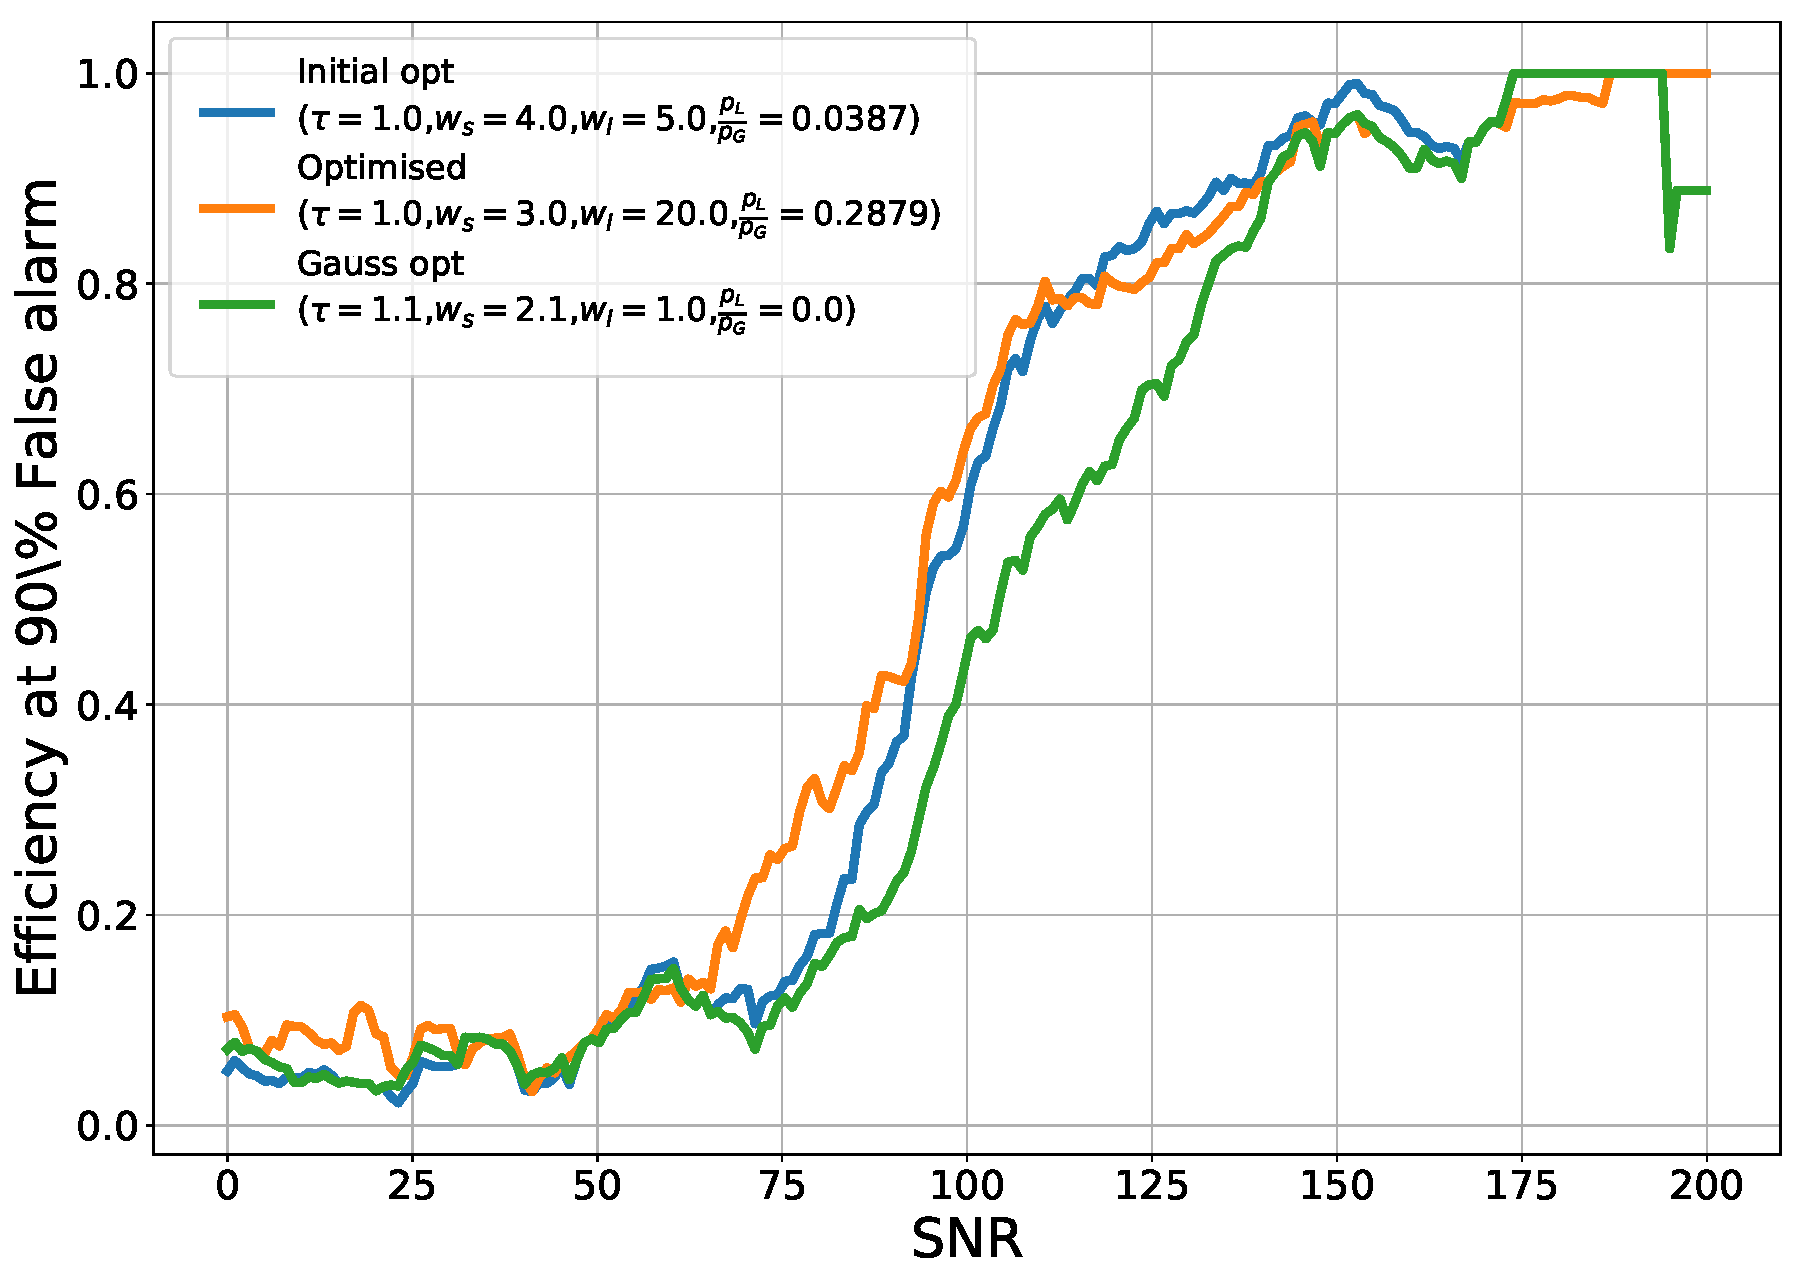
\includegraphics[width=0.9\linewidth]{C3_soap/optimised_comparison.pdf}
	\caption[Comparison of three sets of parameters of the line aware statistic.]{The sensitivity can be compared for three sets of parameters of the line aware statistic. These are the two sets optimised for Gaussian noise and the S6 \gls{MDC} above and the values used in Tab.~\ref{soap:results:parameters}. }
	\label{soap:las:optimisation:comparison}
\end{figure}


\clearpage

%%%%%%%%%%%%%%%%%%5
%%%%%%%%%%%%%%%%%%%
\subsection{\label{soap:sensfreq}Sensitivity with frequency}
%%%%%%%%%%%%%%%%%%%5
%%%%%%%%%%%%%%%%%%%%

All of the above tests, the search was conducted in the range from 100-200 Hz.
This was chosen to be within the most sensitive band of \gls{LIGO} as this is where a signal is most likely to be discovered.
However, signals can appear at much higher frequencies also.
Therefore, it is important to see how the sensitivity of the search varies with the frequency.
 
For this test we simulated \gls{CW} signals in Gaussian noise with no gaps in data. 
The injections used the same source parameters as in the a6 \gls{MDC} \citep{walsh2016ComparisonMethods} and the tests above. 
This has the exception that the integrated recovered \gls{SNR} of the signal is sampled uniformly between 50 and 500. 
These injections were then made at frequencies of 100,250,500,750,1000,1500 and 2000 Hz, where the band width is 2 Hz. i.e. the simulations were in frequency bands 100-102 Hz, 250-252 Hz etc.
The setup of the search was the same as in the above sections. 
Here each sub-band is 0.1 Hz wide, and the parameters of the SOAP search were as in Tab.~\ref{soap:results:parameters}.

Fig.\ref{soap:sens:results} shows the resulting efficiency curves from each of these tests.
This is for a 1\% false alarm rate, which means that 1\% of sub-bands which contained no injection crossed the detection threshold. 
This plot shows how the sensitivity of the search drops as the frequency increases.
This is perhaps unfair to the algorithm as we used the setup of the search which has been optimised for the range 100-200 Hz.
Optimising the search means, choosing the parameters of SOAP, the key parameter which will affect this is the transition matrix. 
As the simulated signals frequency is increased, the scale of the Doppler modulation will also increase.
This means that at higher frequencies the signal is more likely to jump more than a single frequency bin. 
The current setup of the search does not allow this size of jump, therefore, would struggle to identify this type of track.
The other main factor which will decrease this sensitivity is the sub-band width of 0.1 Hz. 
Similarly to before, as the frequency increases the scale of the Doppler modulation will increase as in Eq.~\ref{soap:results:dforbit}.
For example at 1000 Hz, the Doppler shift is $\sim 0.1$ Hz, the signal is then more likely to not be fully contained within a frequency band. 
Therefore, the search can not accumulate all of the injected \gls{SNR}

Whilst these parameters of the search can be changed to depend on frequency, this was meant as a small test to see how sensitivity varies with frequency.


\begin{figure}
	
	\begin{subfigure}[h]{0.9\linewidth}
			\centering
			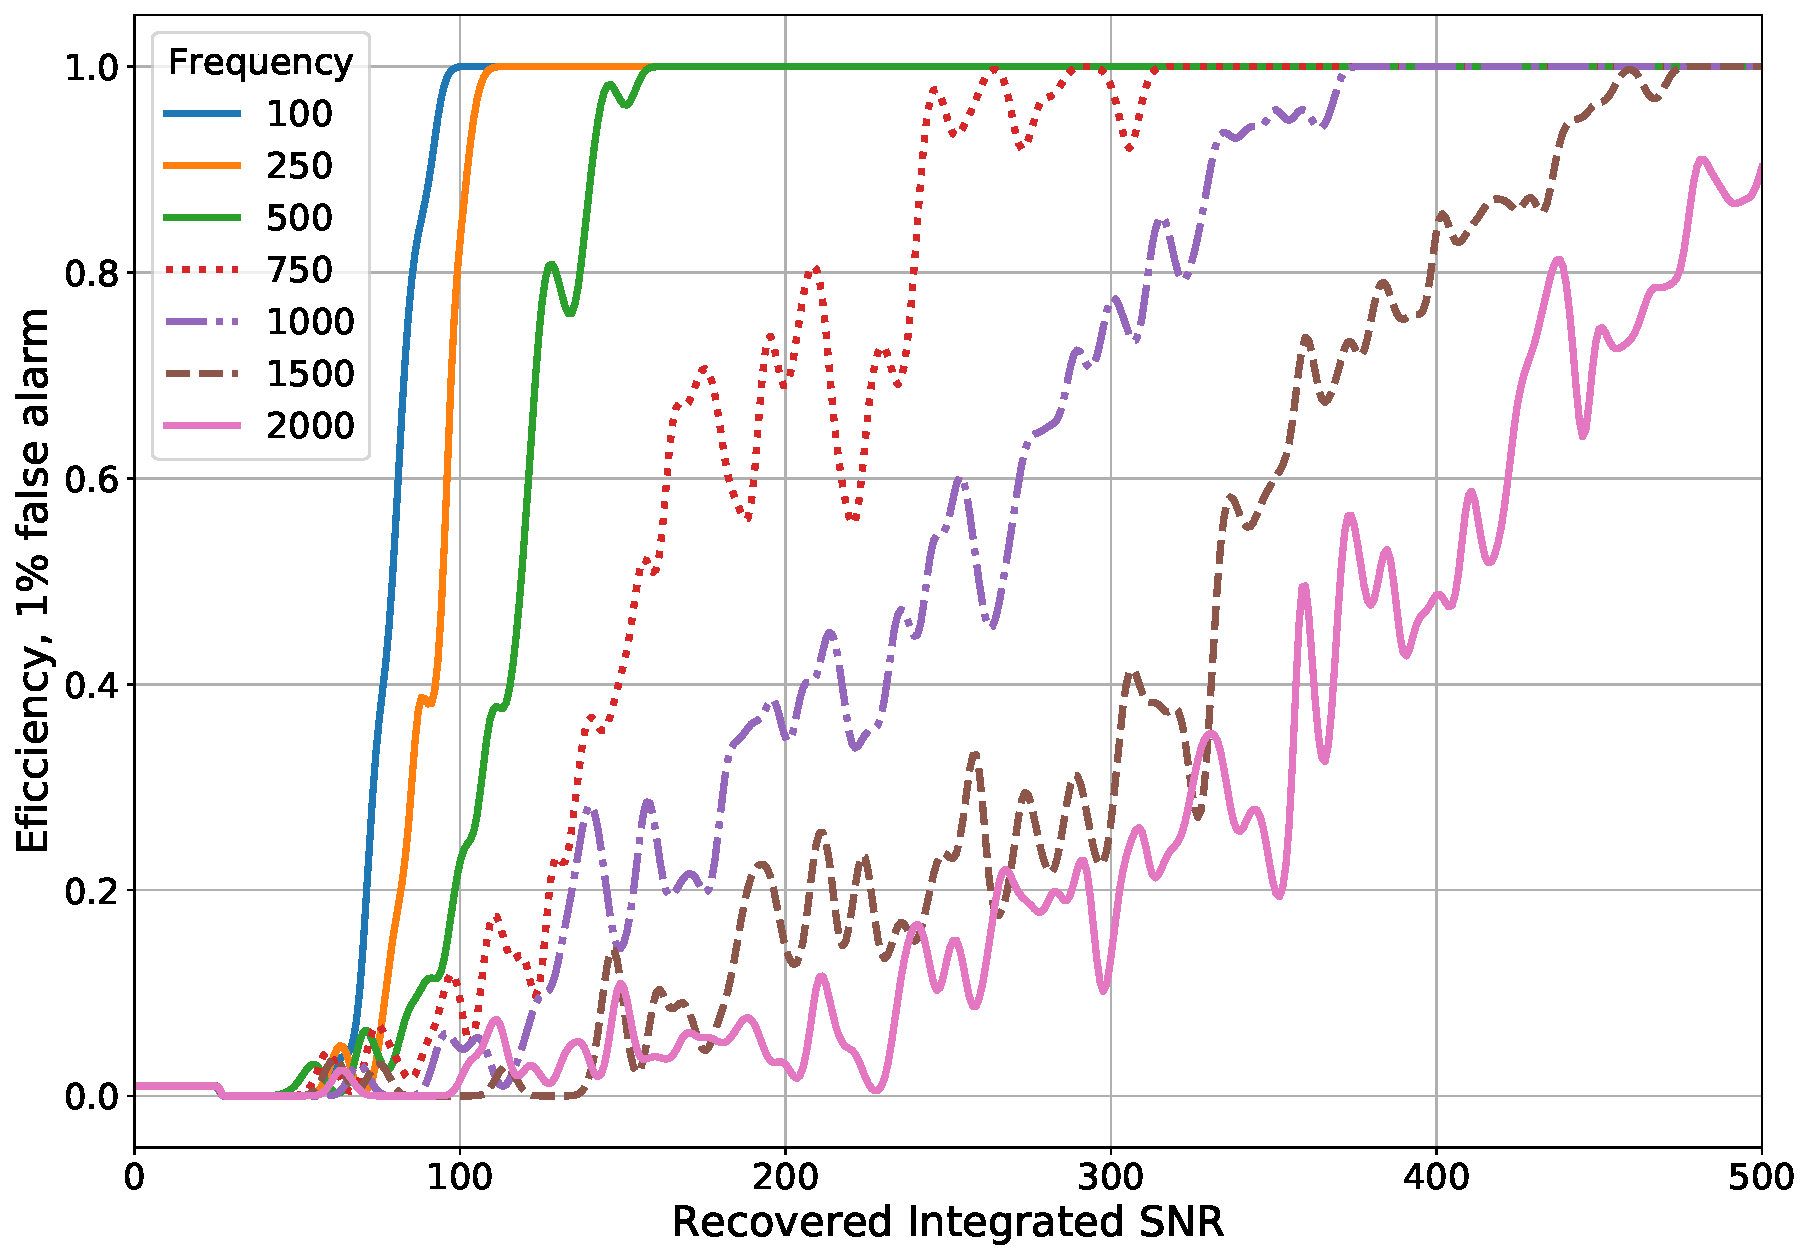
\includegraphics[width=\linewidth]{C3_soap/snr_freq_eff.pdf}
			\caption{}
			\label{soap:sens:eff}
	\end{subfigure}

	\begin{subfigure}[h]{0.9\linewidth}
		\centering
		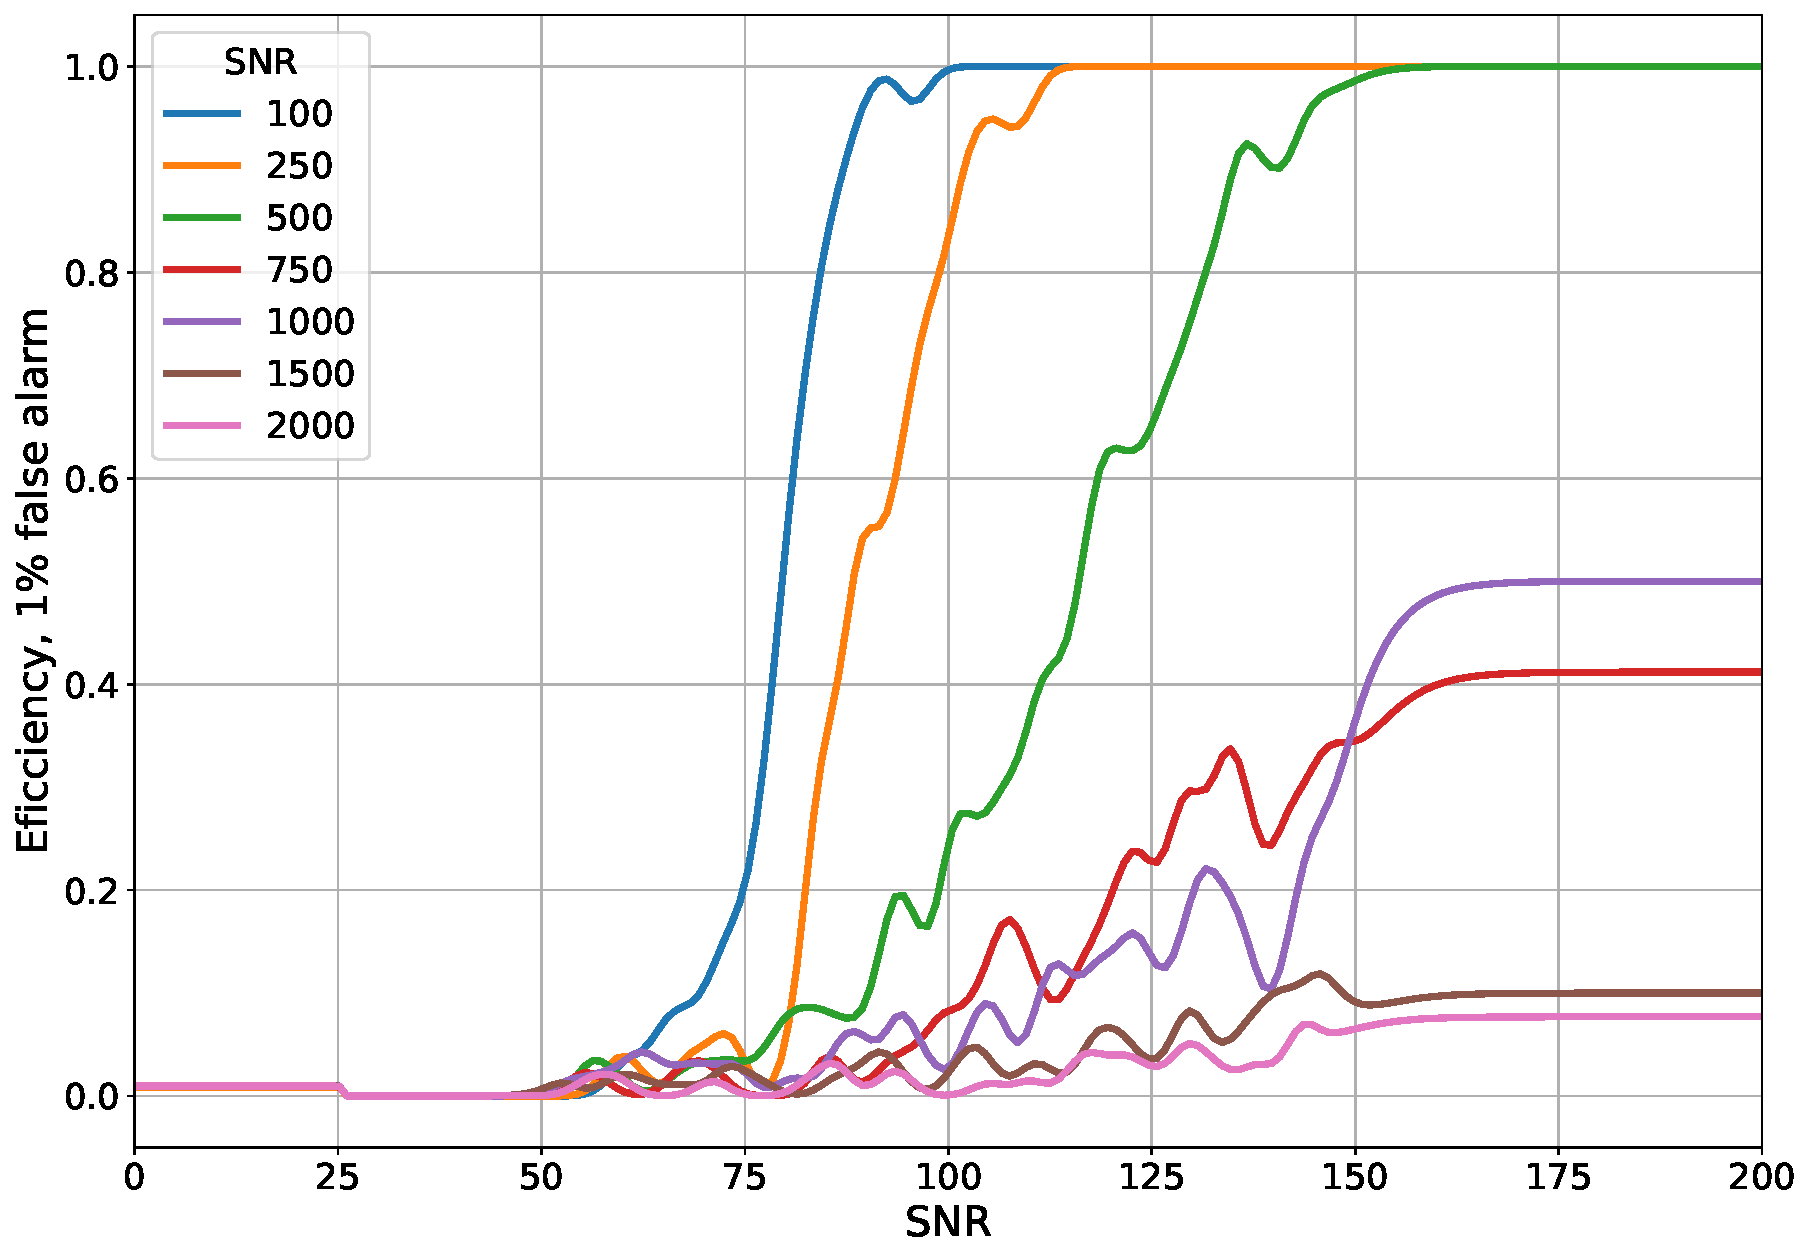
\includegraphics[width=\linewidth]{C3_soap/snr_with_freq.pdf}
		\caption{}
		\label{soap:sens:snrfreq}
	\end{subfigure}

\caption[How the sensitivity of SOAP changes with frequency.]{The sensitivity of the SOAP search in this configuration decreases as the frequency of the pulsar increases. This setup of data for the search however, was optimised for the 100-200 frequency band and can be changed for different frequencies. \ref{soap:sens:eff} shows the efficiency curves with 1\% false alarm rate for each frequency. \ref{soap:sens:snrfreq} shows the values from the efficiency curves at 90\% efficiency.}
\label{soap:sens:results}

\end{figure}


%%%%%%%%%%%%
%%%%%%%%%%%%%%
\subsection{\label{soap:sens:other} Searching for non CW sources}
%%%%%%%%%%%%%%%
%%%%%%%%%%%%%%

Whilst SOAP was designed to search for sources of \glspl{CW}, when set up correctly, it can be applied to searching for other signal types.
This is because the search is essentially un-modelled, and in its simplest form looks for tracks of high power in a spectrogram.
Therefore, if the signal can be represented in a spectrogram, then it can be searched for using SOAP.

\subsubsection{CBC}

CBC signals cover a wide frequency range and are very short signals in \gls{LIGO} detectors. 
The longest of these are \gls{BNS} signals which are on the order of 10 s. 
In previous SOAP searches the default length of \gls{SFT} has been 1800 s, however ,this is not suitable when searching for \gls{CBC} signals.
We then need a shorter time base for each of the \glspl{SFT}, where for following examples these are overlapping in time.
This allows us to achieve the desired time and frequency resolution

Fig.~\ref{soap:sens:other:gw170817} shows an example of the two detector SOAP search running on data +2s and -5 s of the GW170817 merger time \citep{abbott2017GW170817Observation}. 
The spectrograms show the \glspl{SFT} power spectra divided by their median.
Each of the \glspl{SFT} is 0.2 s long and are overlapping by 90\% (0.189 s), this gives a frequency resolution of 5 Hz. 
Whilst this may not be an optimal setup for this particular search, it demonstrates that SOAP can identify a \gls{BNS} signal within the data. 
The example in Fig.~\ref{soap:sens:other:gw170817} show the result between $\sim 20$ and $\sim 520$ Hz, however the SOAP search returns the same track for a wider band-width up to 2000 Hz. 

\begin{figure}[h]
	\centering
	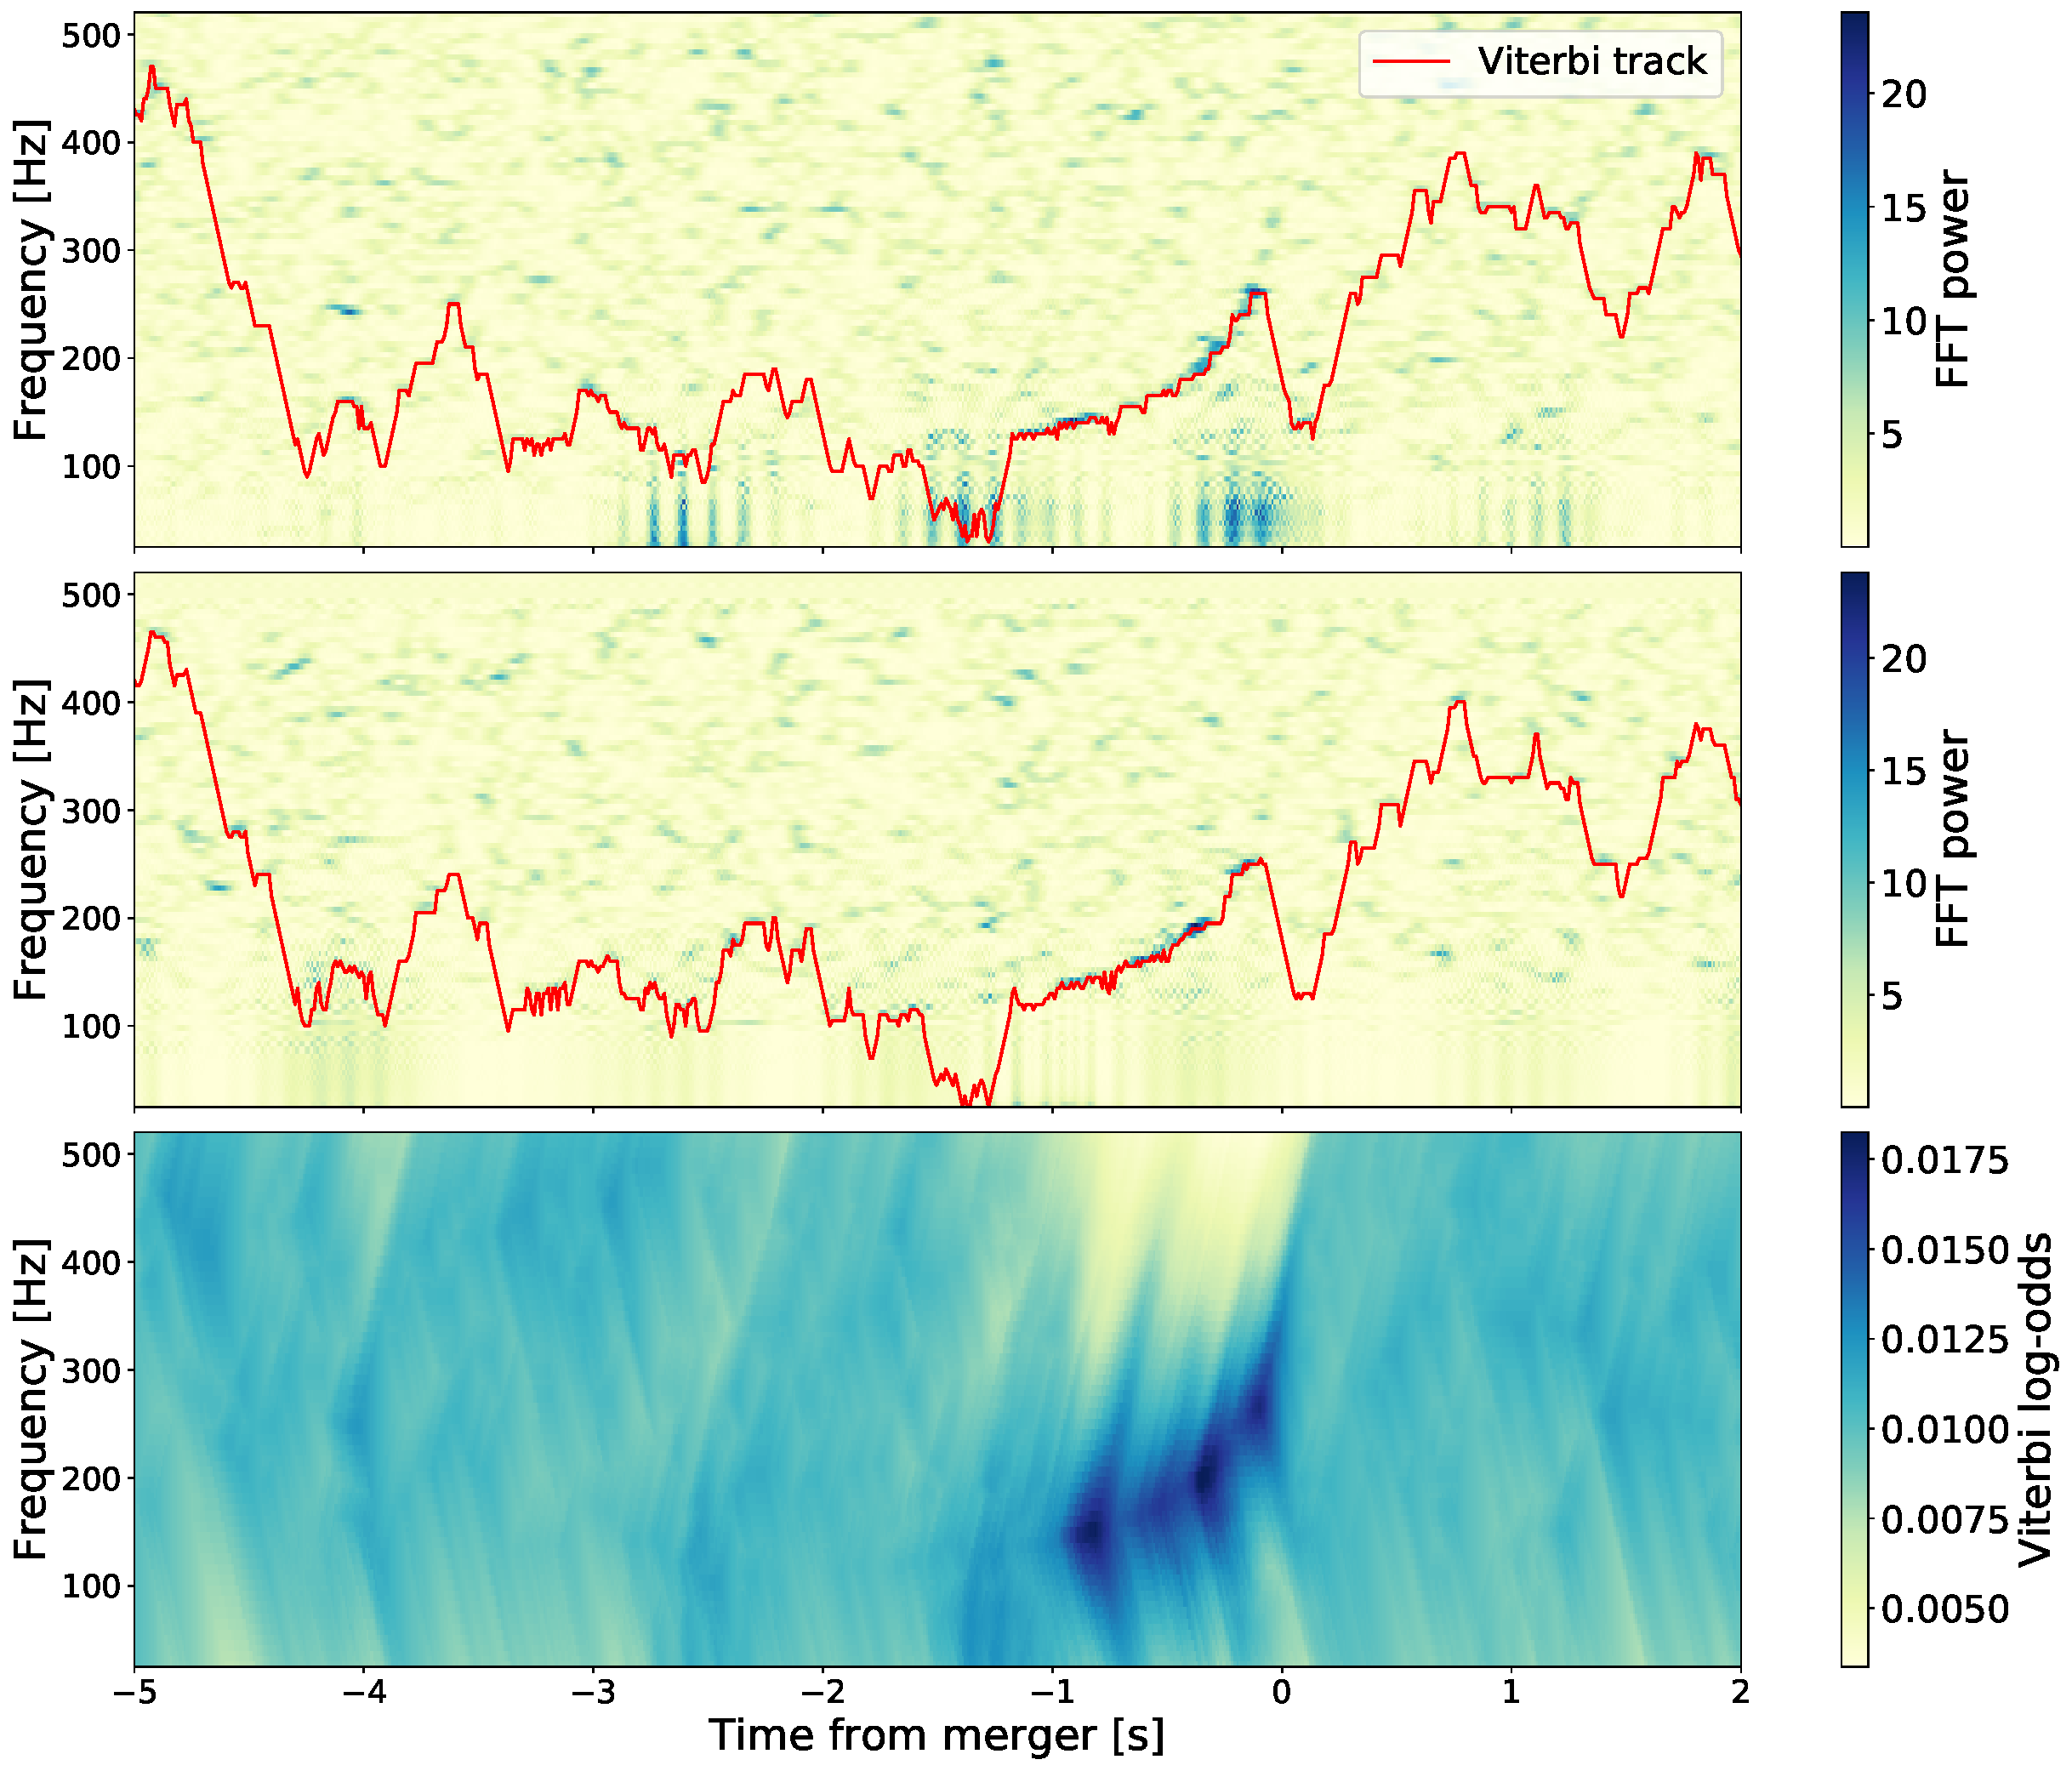
\includegraphics[width=\linewidth]{C3_soap/gw170817_vitplot.pdf}
	\caption[SOAP search run on GW170817]{The SOAP search was run on a spectrogram of \gls{LIGO} data +2 and -5 seconds around the merger of GW170817 \citep{abbott2017GW170817Observation}. Each \gls{FFT} in the spectrograms are 0.2 s long and are overlapping by  0.189 s (95\%). This demonstrates that the SOAP search can identify part of a \gls{BNS} signal within the data, particularly the lower frequency parts.}
	\label{soap:sens:other:gw170817}
\end{figure}

Searching for \gls{BBH} systems becomes more difficult as they are in the \gls{LIGO} band for a short period of time ($ < 1 s$).
To see the evolution of the signal in a spectrogram, the time resolution required means that the frequency bins are too large to see the signals evolution.



%%%%%%%%%%%%%%%%%%%%%%%%%%%%%%%%%%%%%%%%%%%%%%%%%%%%%%%%%%%%%%%%%%%%%%%%%%%%%%%
%%%%%%%%%%%%%%%%%%%%%%%%%%%%%%%%%%%%%%%%%%%%%%%%%%%%%%%%%%%%%%%%%%%%%%%%%%%%%%%
\subsection{\label{soap:results:time}Computational cost}
%%%%%%%%%%%%%%%%%%%%%%%%%%%%%%%%%%%%%%%%%%%%%%%%%%%%%%%%%%%%%%%%%%%%%%%%%%%%%%%
%%%%%%%%%%%%%%%%%%%%%%%%%%%%%%%%%%%%%%%%%%%%%%%%%%%%%%%%%%%%%%%%%%%%%%%%%%%%%%%

One of the main strengths of this search is the drastically reduced computational cost when compared to other current \gls{CW} searches.
The scaling of the computing cost can be estimated for a single detector by looking at the number of calculations that need to be made. 
The number of calculations for a single detector search, $N^{(1)}_{\rm{calcs}}$ is,
\begin{equation}
\label{soap:results:time:singlecalc}
N^{(1)}_{\rm{calcs}} = n_{1}^{m}NM,
\end{equation}
where $n_1$ is the size of the transition matrix, $N$ is the number of \glspl{SFT}, $M$ is the number of frequency bins and $m$ is the amount of memory described in Sec.~\ref{soap:memory}. Where the computing cost scales linearly with the number of frequency bins and \glspl{SFT}.
In the following test we ignore `memory' and look at the time taken for the single detector search where the time taken to read and save data is ignored. Here the data is the same size as the S6 \gls{MDC} for a single detector search and the search is over a 0.1\,Hz band, where we set $n_1=3$. This test, and the following test, was run locally on a MacBook Air with a 1.3 GHz Intel Core i5 processor .We can then write the time taken ,$T$, as,
%
\begin{equation}
T = 0.56\,\rm{sec}\left( \frac{N}{22538}\right) \left( \frac{M}{180}\right) \left( \frac{N_{\rm{bands}}}{1}\right),
\end{equation}

where  $N_{\rm{bands}}$ is the number of different frequency
bands.
For the multiple, $Q$, detector case, we can then generalise Eq.~\ref{soap:results:time:singlecalc} and write the number of calculations $N^{(Q)}_{\rm{calcs}}$ as,
\begin{equation}
\label{soap:results:time:numbercalcs}
N^{(Q)}_{\rm{calcs}} = NMn_{1}^{m} \prod_{q=1}^{Q}n_{q+1},
\end{equation}
where $n_1$ is the first dimension of the transition matrix, $Q$ is the number of detectors and $n_{q+1}$ is the size of the transition matrix element which refers to detector $q$.
For our tests we set $n_1=n_{q+1}=3$ and use 2 detectors i.e., $Q=2$ which each have the same size data as the previous test. The actual time taken to run however, depends on the version of the algorithm which is run. For example, including the line aware statistic slows the search slightly.
For the two detector where two \gls{SFT} powers are summed,
\begin{equation}
T = 1.35 \rm{s}\left( \frac{N}{22538}\right) \left( \frac{M}{180}\right) \left( \frac{N_{\rm{bands}}}{1}\right).
\end{equation}
The same search now including the line aware statistic, which is implemented using a lookup table, changes this to,
\begin{equation}
T = 25.7 \rm{s}\left( \frac{N}{22538}\right) \left( \frac{M}{180}\right) \left( \frac{N_{\rm{bands}}}{1}\right).
\end{equation}

Other searches, excluding Einstein@home which takes on the order of months to run ( $>100$ million core-hours \citep{walsh2016ComparisonMethods}), take $1-10$ million core-hours \citep{walsh2016ComparisonMethods}. This search should take $\mathcal{O}(10^3)$ core-hours.

%%%%%%%%%%%%%%%%%%%%%%%%%%%%%%%%%%%%%%%%%%%%%%%%%%%%%%%%%%%%%%%%%%%%%%%%%%%%%%%
%%%%%%%%%%%%%%%%%%%%%%%%%%%%%%%%%%%%%%%%%%%%%%%%%%%%%%%%%%%%%%%%%%%%%%%%%%%%%%%
\section{\label{soap:dicussion}Discussion}
%%%%%%%%%%%%%%%%%%%%%%%%%%%%%%%%%%%%%%%%%%%%%%%%%%%%%%%%%%%%%%%%%%%%%%%%%%%%%%%
%%%%%%%%%%%%%%%%%%%%%%%%%%%%%%%%%%%%%%%%%%%%%%%%%%%%%%%%%%%%%%%%%%%%%%%%%%%%%%%

In this paper we describe an application of the Viterbi algorithm, called SOAP, to
search for continuous sources of gravitational waves.
This paper outlines the method and derives the statistics behind the method in a consistent Bayesian formalism. It then presents the results from the first set of tests of sensitivity for the SOAP algorithm on three separate datasets.

%
% overview of results from tests
%
We tested SOAP on a set of fake isolated pulsar signals in the
100\;--\;200\,Hz range, based on 1800s \glspl{SFT} summed over one day.
The three datasets that included these signals comprised continuous Gaussian noise, Gaussian noise but with temporal gaps corresponding to LIGO dead times in the S6 data run, and real data, i.e., the
S6 \gls{MDC}. Although a major attraction of SOAP is its sensitivity to a wide
range of signal types, in the tests above it was optimised to detect isolated pulsar signals below 100\,Hz with low spin-down to offer a comparison with other \gls{CW} searches. From these tests, by setting a
95\% efficiency and a false alarm of 1\%, we found that in the case of  continuous Gaussian data we could detect a signal with an optimal \gls{SNR} of $\sim 60$ and a
depth of $\sim 33$\,Hz$^{-1/2}$ with an \gls{RMS} of the difference between the injected and Viterbi track being $\sim 2$ frequency bins (0.0012 Hz).
When gaps were introduced into the data to simulate S6 we could detect a signal with an
\gls{SNR} $\sim 72$  and a depth of $\sim 10$\,Hz$^{-1/2}$, with an \gls{RMS} of $\sim 10$ bins (0.0056 Hz). The drop in sensitivity here is simply because  there is $\sim 50 \%$ less data compared to the previous case. Finally, in the S6 \gls{MDC} we could
detect a signal with an \gls{SNR} $\sim 74$ and a depth of $\sim
13$\,Hz$^{-1/2}$.
These real data contain non-Gaussian artefacts such as instrumental lines and this causes a further drop in sensitivity.
Whilst not a full comparison to other searches in the S6 \gls{MDC} \citep{walsh2016ComparisonMethods}, as we only tested on a subset
of the bands, this search has a sensitivity which is comparable to some other \gls{CW} searches, however offers a massive increase in speed.

We chose the specific frequency band to search over as the data which we used, i.e., the summed data, becomes less effective at frequencies much higher than 200\,Hz, and using the parameters of our simulations, signals can spread over many frequency bins in a day, reducing sensitivity further, however this can be mitigated by using shorter \glspl{SFT} or performing their summation over 12 (rather than 24) hours.

%
% some other features to test in the future
%
The methods described in this paper present a basic approach for gravitational-wave signal searches using SOAP. However there are several further developments that could increase its sensitivity. Some of these are outlined below:

One of the main features which reduces the sensitivity of the search is non-gaussianities within the data, namely instrumental lines. Although we have a statistic which penalises these features, in some cases it will also penalise a strong signal. For example, when the amplitude of the noise floor is high for one detector or the duty factor is lower, the signal will appear more like an instrumental line to this statistic. We hope to improve the search statistic in the future by searching for consistent amplitudes as opposed to consistent \gls{SNR}, i.e, the statistic will take the amplitude of the noise floor and the duty factor into account.

One variation of this method which has been described in this paper is `memory', which is where the tracks jump in frequency is determined by the previous $n$ jumps. This has yet to be fully tested, however, we expect that this will increase our sensitivity to signals where have a better idea of their frequency evolution. This however, comes at a cost in computational time which we can estimate given Eq.~\ref{soap:results:time:numbercalcs} in Sec.~\ref{soap:results:time}.

Further additions to the search include using the Fourier transform of the \gls{SFT} power along the Viterbi track as a detection statistic.
If the Viterbi track follows that from an astrophysical signal, then we should see the effects of the antenna pattern in this Fourier transform as a peak at half a sidereal day.
If the track follows something which is not astrophysical then this should not be seen this peak in this Fourier transform.
This only applies to the search directly on the \glspl{SFT} not the summed data, as the antenna pattern variations will have been averaged out in the summing.

As well as searching for astrophysical signals, SOAP can also be used to search for and identify instrumental lines. Here we use single detector data, or multiple channels from a single detector, to identify quasi-monochromatic features on the data for further study.

Whilst this paper presents initial tests on sensitivity, further tests will be needed for a full comparison to other \gls{CW} search methods.  
This search, however, aims to look for signals which may not follow the standard
frequency evolution and is intended to return potentially interesting
candidates for a more sensitive followup.



\chapter{\label{machine} Machine learning for continuous wave searches}
%%%%%%%%%%
%%%%%%%%%%

%--------------------------
% Introduce machine learning
%----------------------------

Machine learning is a term which was used by Arthur Samuel in 1959. 
He described it as a "Field of study that gives computers the ability to learn without being explicitly programmed" \citep{}.
This can be though of as a subset of artificial intelligence. 
With the development in computing in recent years along with the easier access to large data-sets, machine learning has become much more accessible.
One machine learning technique which is widely used is deep neural networks. 
There are used extensively in classification problems as well as others.
\joe{want to write a little bit more here}

%------------------------
%Overview of what is paper and not
%--------------------------
This chapter aims to given an overview of neural networks, specifically \glspl{CNN} and their application to a \gls{CW} search. 
The majority of this section is written in a paper which is yet to be published, however, is aimed to be submitted soon.
The differences are, Sec.~\ref{machine:nn}, \ref{machine:cnn} and \ref{machine:training} which describe the operation of neural networks have more detail in this thesis than in the paper draft. 
Sec.\ref{machine:results:sens_size} is additional material which is currently not included in the paper draft.


%%%%%%%%%%%%
%%%%%%%%%%%%%%%
\section{\label{machine:intro} Introduction}
%%%%%%%%%%%%
%%%%%%%%%%%%%

% Intro to GWs and CW
%
Gravitational wave detectors such as \gls{LIGO}~\cite{abbott2009LIGOLaser,aasi2015AdvancedLIGO} and VIRGO
\cite{acernese2015AdvancedVirgo,acernese2008StatusVirgo} search for a number of different targets. 
Some targets such as \glspl{CBC} have been observed ~\cite{abbott2017GW170817Observation,abbott2017GW170814ThreeDetector,abbott2016ObservationGravitational},
however, other primary sources such as \glspl{CW} are yet to be observed.
\glspl{CW} are well modelled quasi-sinusoidal signals with a
duration much longer than observing times of detectors.
The source of these signals is thought to be rapidly rotating neutron stars which can emit \gls{GW} if there is some asymmetry around its rotation axis. 
This can be caused by various mechanisms as described in ~\cite{prix2009GravitationalWaves}. 
These signals have small amplitude, which if detected will be below the noise \gls{PSD} of the detector.
Therefore, sensitive search algorithms are needed to find the signals. 
These algorithms generally fall into three categories: Targeted,
directed, and all-sky searches, listed in order of how much is known a priori
about the source from \gls{EM} observations. 

% describe the different general types of CW search
%
In targeted searches the sky position, frequency, and its derivatives are
assumed to be well known, in directed searches only the sky position is
known and in all-sky searches the sky position and frequency of the source is unknown.
The most sensitive of these are targeted searches which use coherent matched
filtering~\cite{dupuis2005BayesianEstimation,schutz1998DataAnalysis}. These use
template waveforms which are generated using the information already known about the
source, then correlated this with the data. Directed and all-sky searches have
a much broader parameter space to search, therefore, many templates are needed
to sufficiently cover the parameter space. Using the coherent matched filter
for broader parameter space searches becomes unfeasible due to the amount of
computing time that is needed. This led to the development of semi-coherent
searches where the data is divided up into smaller segments which can be analysed
separately and then the results can be recombined incoherently using various
methods~\cite{abbott2019AllskySearch,creighton2000SearchingPeriodic}. Semi-coherent
searches result in a trade off between sensitivity and computing time.

% Introduce SOAP and explain the line artefact problem
%
The analysis here is presented mainly as an addition to an existing
semi-coherent search algorithm titled SOAP~\cite{bayley2019SOAPGeneralised}.
This is a fast and largely un-modelled search which finds tracks of
high \gls{FFT} power in time-frequency spectrograms. 
When applied to multiple detectors using a line-aware statistic, SOAP looks for frequency bins which have both a high power and are similar in each detector. 
This means that  at a given frequency at a given time, SOAP will penalise frequencies where the \gls{FFT} power is largely different in each detector.  
The algorithmic details summarised in Sec.~\ref{soap}. 

% instumental lines and how the affect SOAP
%

One effect which limits the sensitivity of SOAP and many other
\gls{GW} searches is noise artefacts known as `instrumental lines'. These can be anything
from long duration fixed frequency or wandering lines to shorter duration fixed frequency transients. 
There are certain types of instrumental line which the SOAP search can struggle to distinguish from an astrophysical signal even with the development of a
`line aware' statistic in~\cite{bayley2019SOAPGeneralised}. Currently the
method used to reduce the effect of these lines is to manually look at the SOAP
output and the spectrograms for each sub-band to determine whether the sub-band
is contaminated by instrumental effects. This process is slow, requires a
lot of human input and is subject to human error. When the search runs over
a larger bandwidth, it will no longer be practical to look
through all bands. 

% Convolutional neural networks
%

We aim to automate how the search deals with instrumental lines by using \glspl{CNN}.
These have been used extensively in image classification and we explain this in
more detail in Sec.~\ref{cnn}. \glspl{CNN}
have already been shown to detect gravitational wave signals from \glspl{CBC}
in~\cite{gabbard2018MatchingMatched,george2018DeepLearning,gebhard2019ConvolutionalNeural}
and other deep learning techniques have been used in searching for \gls{CW}
signals in~\cite{dreissigacker2019DeeplearningContinuous}. 

% structure of the paper
%
In Sec.\ref{cnn:soap} we will summarise the basics of how the SOAP search works. In
Sec.~\ref{machine:nn}, \ref{machine:cnn} and \ref{machine:training} we explain how \glspl{CNN} operate and how they are trained. Sec.~\ref{machine:cw} will describe how this is applied to an \gls{CW} search. 
This includes the structure of the \gls{CNN} in Sec.~\ref{machine:cw:structure} and the entire search from raw data to results in Sec.~\ref{machine:pipeline}. Finally in Sec.~\ref{machine:results} we
show the results from this search and compare to similar analyses. 

%%%%%%%%%%%%%%%%%%%%%%%%%%%
%%%%%%%%%%%%%%%%%%%%%%%%%%
\section{\label{cnn:soap} SOAP}
%%%%%%%%%%%%%%%%%%%%%%%%%%
%%%%%%%%%%%%%%%%%%%%%%%%%%%

% introduce SOAP and show example of outputs
%
SOAP~\cite{bayley2019SOAPGeneralised} is an un-modelled search for long
duration signals which is based on the Viterbi
algorithm~\cite{viterbi1967ErrorBounds}. In its most simple form SOAP
analyses a spectrogram to find the time-frequency track which gives the highest
sum of \gls{FFT} power. If a signal is present and sufficiently loud then this
is the track which is most likely to come from some signal.
In~\cite{bayley2019SOAPGeneralised} the algorithm has been expanded to
search through multiple detectors as well as including a statistic to penalise
artefacts in the data from the instrument as opposed to from an astrophysical
source. 

% refer to the figure showing the Viterbi track for S6
%
Fig.~\ref{soap:viterbiplot} shows an example of the spectrogram data which is
searched through and the outputs of SOAP; the three main output components are
the frequency track, the Viterbi statistic and the Viterbi map.

\begin{figure}[h]
	%\centering
	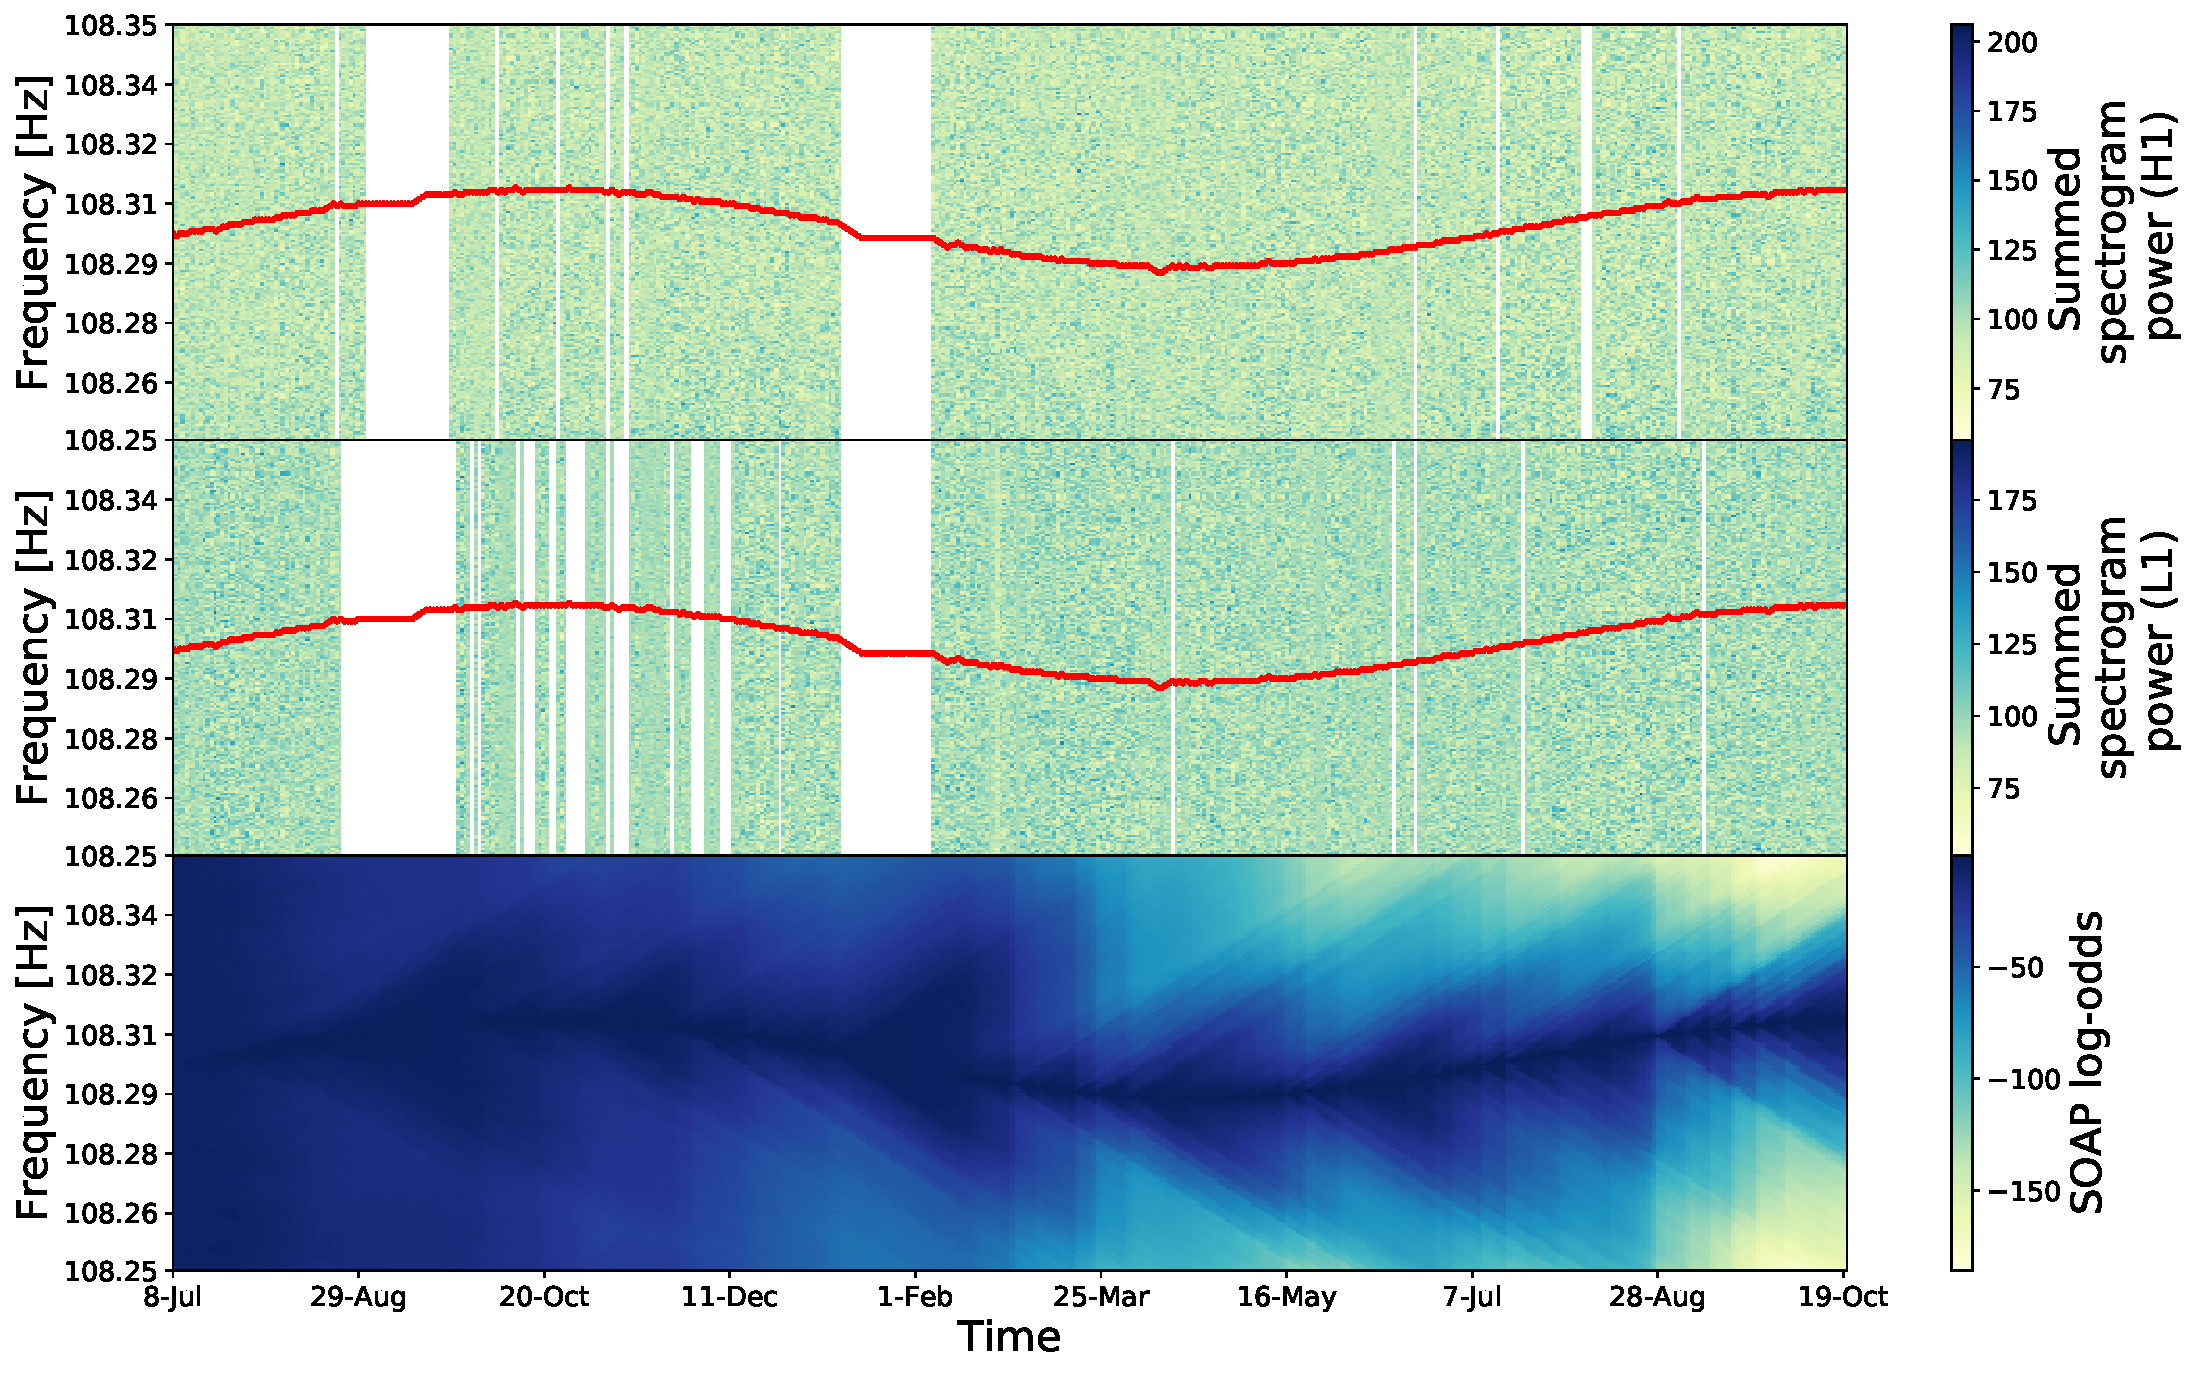
\includegraphics[scale=0.43]{C4_cnn/two_vit_example.pdf}
	%
	\caption{\label{soap:viterbiplot} This plot shows the inputs and outputs of the
		SOAP search. The top two panels are time-frequency spectrograms which have been pre-processed as described in Sec.~\ref{machine:pipeline}. This
		data is a 0.1 Hz wide frequency band from the S6 observing run \cite{} \joe{reference} which includes a string simulated \gls{CW} signal. The white areas in the spectrograms are gaps in data when the detector was not operating. These both have the
		optimal track found by SOAP overlaid. The bottom panel shows the normalised Viterbi map, the intensity of a
		pixel in this image relates to the log-probability that a track ends in and
		particular frequency bin at a given time.}
	%
\end{figure}

% describe the main data products from the search
%
\begin{description} 
	%
	\item [Viterbi track] The Viterbi track is the most probable track through time-frequency data given a choice of statistic. 
	%
	\item [Viterbi statistic] The Viterbi statistic is the sum of the individual statistics along the Viterbi track. In the analysis that follows, the `line-aware' Viterbi statistic is used. 
	This is the sum of the log-odds ratios, $p_{\rm signal}/(p_{\rm line} + p_{\rm noise})$ along the track. This is defined in more detail in \cite{bayley2019SOAPGeneralised}
	%
	\item [Viterbi map]
	The Viterbi map value of the Viterbi statistic for every time-frequency bin in the spectrogram. 
	This represents the most probable track which ends in any time-frequency bin.
	In the Viterbi maps, each time slice is normalised individually, i.e., each
	vertical slice has been normalised such that the sum of their exponentiated
	values is equal to 1. This way each pixel in the image can be interpreted as a
	value related to the log-probability that there is a signal in the bin at that
	time.
	%
\end{description}

% Mention line aware statistic
%
To determine whether an simulated astrophysical signal has been detected,
in~\cite{bayley2019SOAPGeneralised} we used the Viterbi `line aware' statistic alone described above.  
The `line-aware' statistic reduced the affect of instrumental lines on the analysis, however the `line-aware' statistic is still contaminated by certain types of line.
For example, the statistic is affected by broad wandering lines as they offer high power tracks in both detectors.
To reduce the effect of these instrumental lines, we looked through the spectrograms and
Viterbi maps of individual bands by eye as in Fig.~\ref{soap:viterbiplot}.
Bands which appeared to be contaminated were then removed from the search.

% what was different in this analysis
%
In this search the spectrograms and the Viterbi map contained extra information
over the Viterbi statistic. 
We aim to utilise this in addition to the Viterbi statistic to replace the process of removing contaminated bands `by eye' and therefore automating the search. 
A useful tool which can be used to classify this extra information is convolutional neural networks. 

%%%%%%%%%%%
%%%%%%%%%%%
\section{\label{machine:nn}Neural networks}
%%%%%%%%%%%
%%%%%%%%%%%


Throughout this section I will summarise one machine learning technique which are known as Neural networks. 
Neural networks, as the name may suggest, was developed as a way for a computer to mimic the neurons in the brain.
To understand why this would be useful, a common example used is the ability for an algorithm to identify hand written digits.
This seems like a simple task as a brain can complete with ease. 
However, writing a traditional algorithm to perform this same task is very difficult. 
The algorithm would have to identify a particular shape which has a huge amount of variation.
Neural networks offer a way to deal with this problem as they can be trained on large datasets.
This is similar to how a human brain is `trained'. 
In a lifetime of a brain many examples of different symbols are seen and each time a new one is seen the brain `updates' itself based on what is observed. 
This process is essentially replicated for a neural network, where the algorithm can be updated such that it can correctly identify each digit.

This process can be replicated in a neural network, where it has many parameters which can be modified or `trained'. 
These parameters and their application are grouped into objects called neurons, many of these neurons are used to build a neural network.

%%%%%%%%%
%%%%%%%%%
\subsection{\label{machine:nn:neuron}Neurons}
%%%%%%%%%
%%%%%%%%%

Neurons are the building blocks of any neural network.
They perform simple operations on any number of input values and then output a single value.
The output $o$ of a neuron is defined by the equation,

\begin{equation}
    o = f\left(b + \sum_{i=1}^{N} w_i x_i  \right),
    \label{machine:nn:neuron:equation}
\end{equation}

where $b$ is the bias, $x$ is the input, $w$ is the weights, $f$ is the activation function, $o$ is the output and $N$ is the number of inputs.
Here the input $x$ represents either the data which is input, i.e the pixels of the image which contains the digit in the example above, or the output of another neuron.
The weights $w$ then represents how important each of those data points are to this problem, or specifically this neuron. 
The bias $b$ is then just an extra factor which can shift the data by a fixed value.
The activation function $f$ is then a function which can have many forms, in the simplest case in a neuron known as a `perceptron', it provides a cut where any value above a given threshold is 1 and any below is 0, this will be explained in more detail in Sec.~\ref{machine:nn:activation}. 
However, there are many different types of activation functions which can be applied to different situations.
This will be explained in more detail in Sec.~\ref{machine:nn:activation}.

\begin{figure}[h]
    \centering
    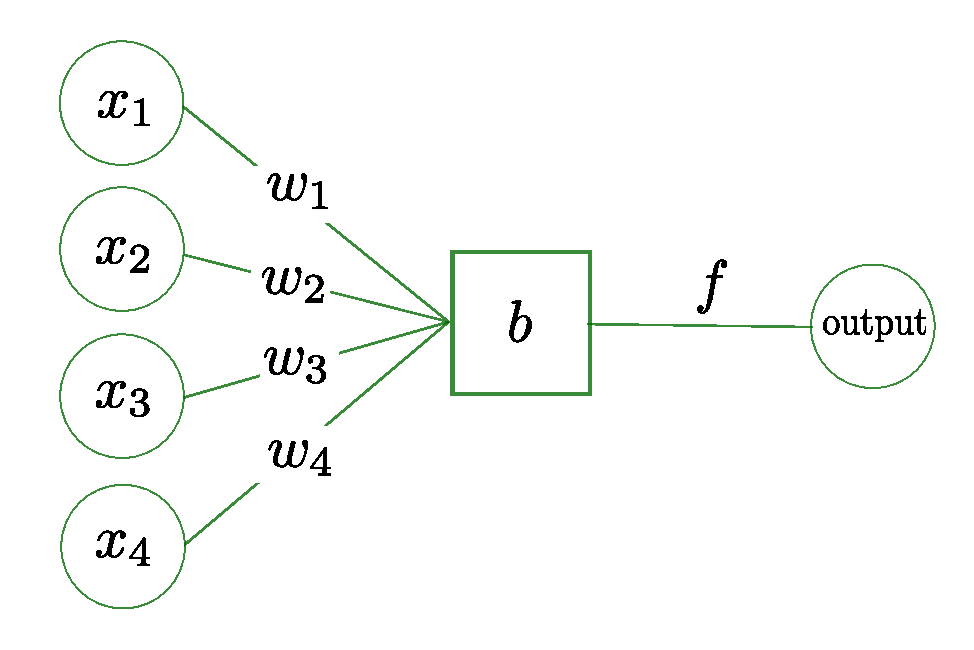
\includegraphics[width=0.6\columnwidth]{C4_cnn/neuron.pdf}
    \caption{Basic neuron}
    \label{machine:nn:neuron:plot}
\end{figure}

In the example in Fig.~\ref{machine:nn:neuron:plot} I have shows a neuron which has 4 input variables, or 4 input data points. 
When a network is trained, or when it learns, the weights applied to each of the inputs and the bias are updated to better represent the input data.
This training procedure is explained in more detail in Sec.~\ref{machine:nn:training}
Many neurons are then used in combination with each other to develop a neural network which can be applied to more complex problems.

%%%%%%%%%%%%%%%%%%%%
\subsection{\label{machine:nn:structure}Network structure}
%%%%%%%%%%%%%%%%%%%%

The structure of a neural network is defined by the user and there is no set way to design a network.
However, the general layout of a neural network is defined by structures called layers, sometimes known as fully connected layers. 
These are rows of $N$ neurons which all take the same input such that there is $N$ output values.
An example of a simple neural network is shown in Fig.~\ref{machine:nn:structure:plot}.
The first layer is the input layer, this is just the data points from an input example.
In the example of hand drawn digits, this would be the pixels from the image of the digit.
The final layer represents the information that you intend the network to extract from the input data. 
In the hand drawn digit example, this could have 10 output values corresponding to each digit 0-9. 
Each of these outputs is then a value which is related to the probability of that digit being present in the image.  

When designing a network, the user will have a defined input layer size from the data and a set number for the output layer which represents, for a classification example, the number of output classes. 
The number of hidden layers and the number of neurons in those hidden layers can be arbitrarily changed. 
In general if the data contains more complex information the size or complexity of the network will need to be increased for it to be able to extract the information. 
If there is a small number of training examples and a large and complex network, it may be able to learn the input data set as opposed the the general information that they represent.

\begin{figure}[h]
    \centering
    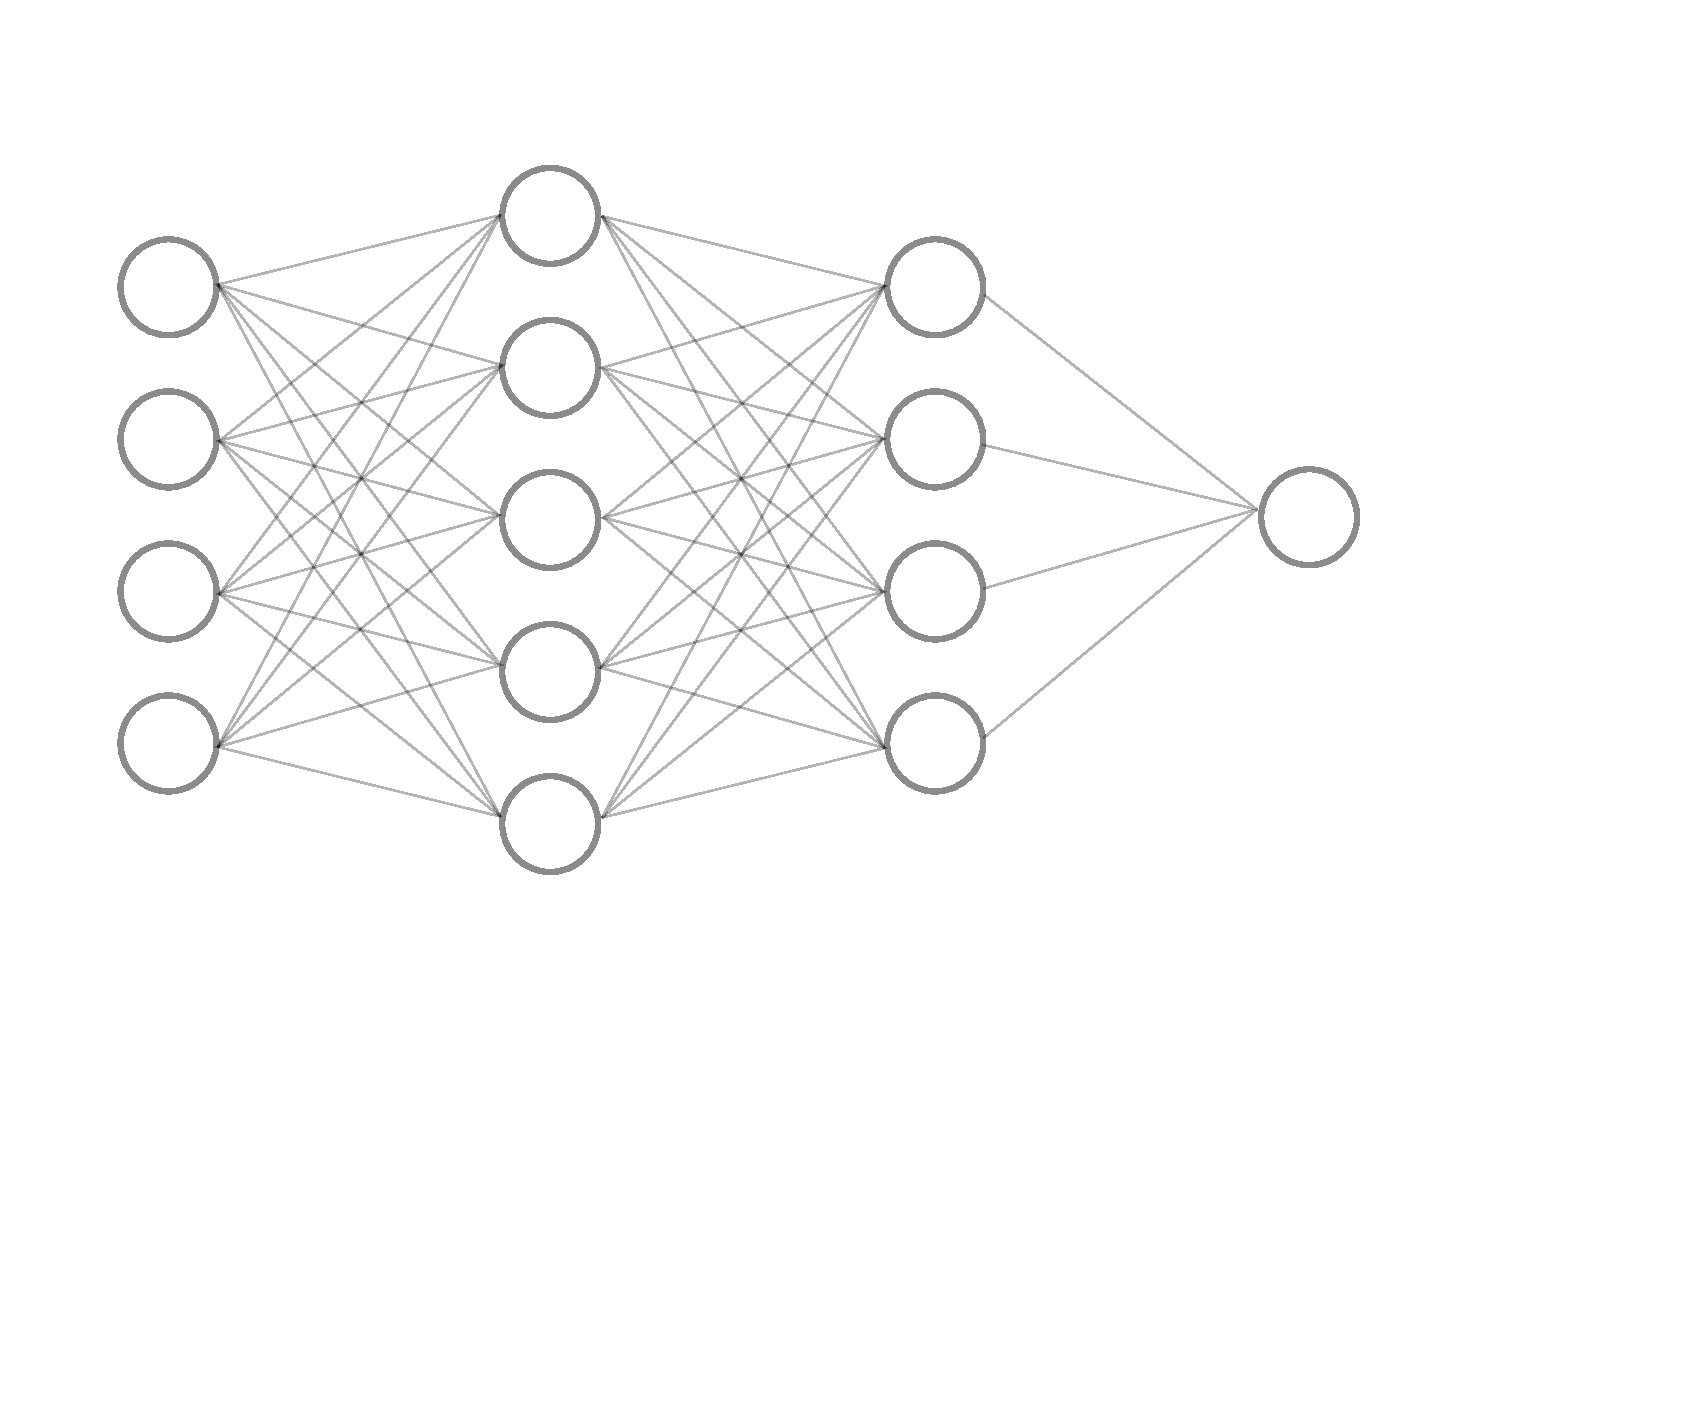
\includegraphics[width=\columnwidth]{C4_cnn/simple_network.pdf}
    \caption{A neural network is structured with layers. Each of the circles in these layers are neurons as described in Sec.~\ref{machine:nn:neuron} and Fig.~\ref{machine:nn:neuron:plot}. The networks contain an input layer which is usually the data which you would like to analyse. Then this passes to a number of `hidden' layers, in the above diagram there are two. Hidden layers are just layers which exist between the input and the output. The output layer is then the desired output, above I have chosen a single neuron as output. This is such that the network could classify the input to a value between 0 and 1. Every neuron in a layer is connected to the output of all neurons in the previous layer.}
    \label{machine:nn:structure:plot}
\end{figure}


%%%%%%%%%%%%%%%%%
\subsection{\label{machine:nn:activation}Activation functions}
%%%%%%%%%%%%%%%%%

The activation function is how the output of a neuron is transformed. 
The most simple activation function is a cut as described in Sec.~\ref{machine:nn:neuron}, however, this type of activation does not perform well.
Activations functions a generally based on a few properties.
The activation function is generally non-linear, this allows networks with multiple layers to be used to approximate a function. A linear activation function means that any number of layers in a network is equivalent to a single layer network.
Another property which is desired in activation function is that it is continuously differentiable. This is to allow algorithms such as gradient descent to optimise the network. 
The functions are found to perform better if they are monotonic and smooth.
There are many choices when defining this in the network, some of the available options are shown in Fig.~\ref{machine:nn:activation:plot}.
One of the more commonly used activation function is the LeakyRELU function, this is explained in more detail in \citep{maas2013RectifierNonlinearities}.
In the work that follows we use the Leaky RELU function and the sigmoid function.


\begin{figure}[h]
	\centering
	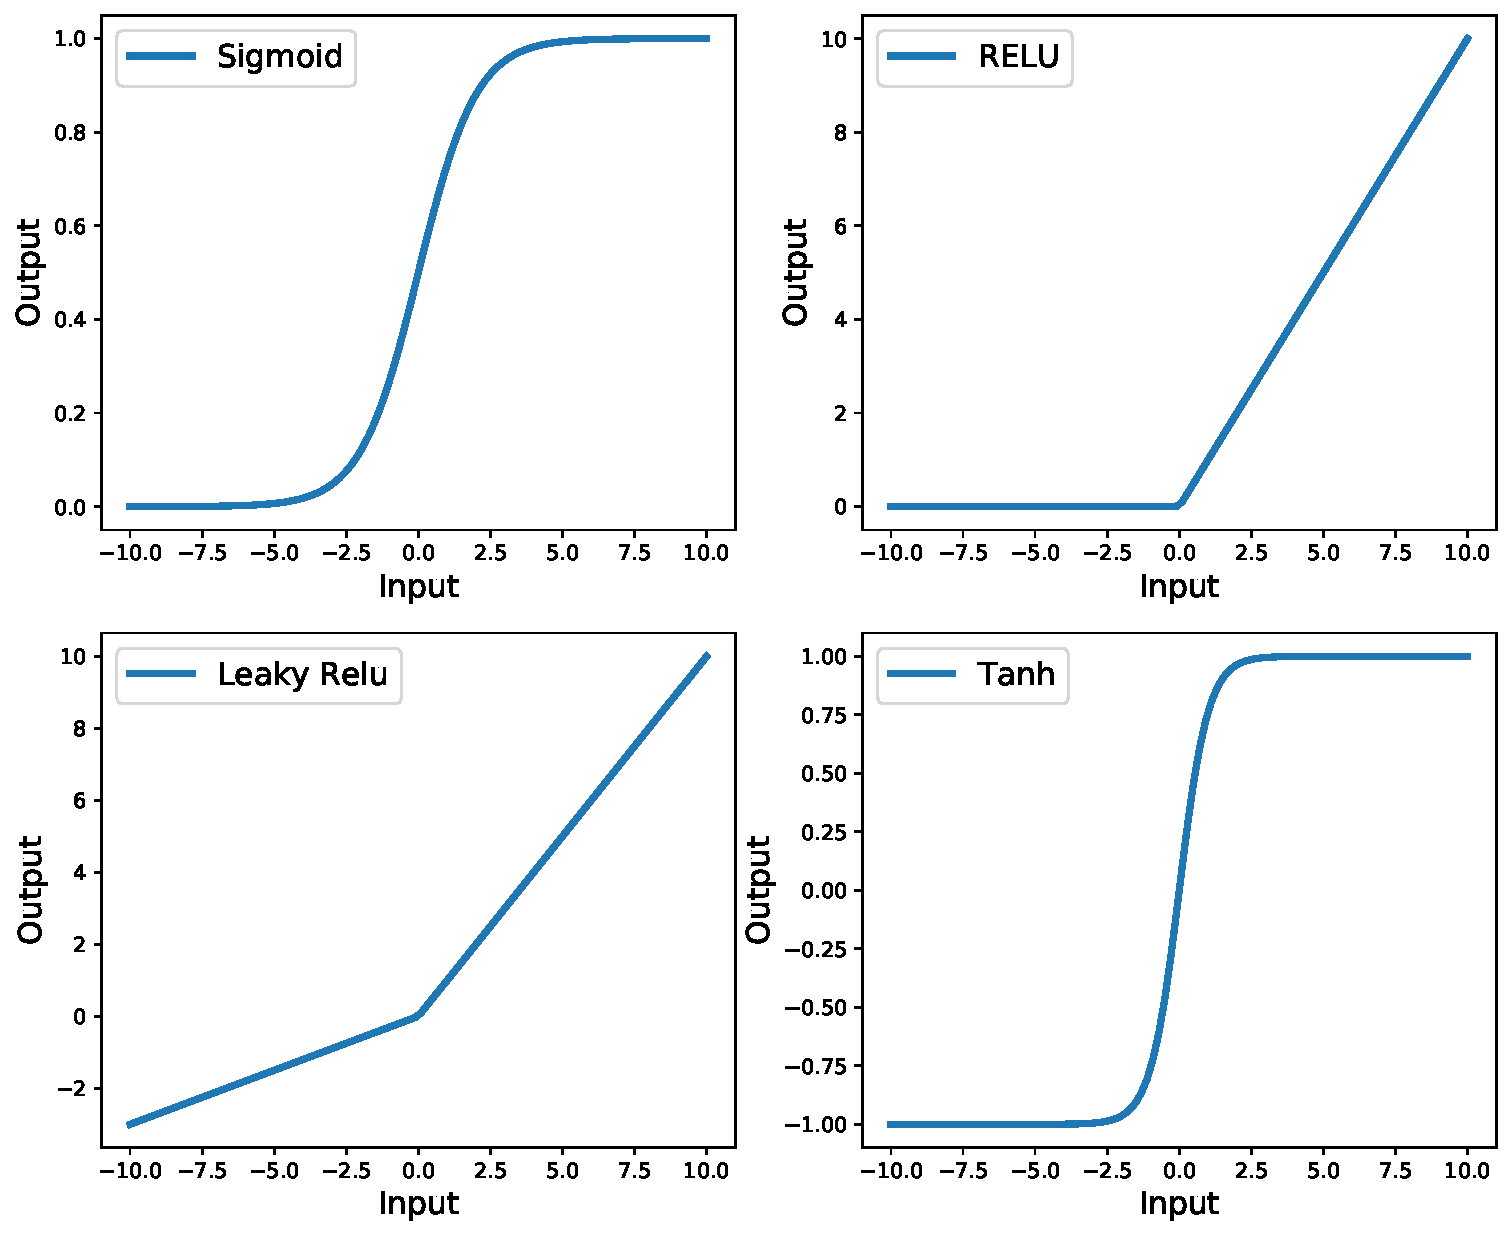
\includegraphics[width=0.8\columnwidth]{C4_cnn/activations.pdf}
	\caption{There are many different activations function which are used, and essentially any function can be defined if necessary. Above is shown a subset of the more commonly used functions. The linear function is not used, however, is there to compare to common non linear function.}
	\label{machine:nn:activation:plot}
\end{figure}





%%%%%%%%%%%
%%%%%%%%%%%
\section{\label{machine:cnn}Convolutional Neural Networks}
%%%%%%%%%%%
%%%%%%%%%%%

\glspl{CNN} are a different type of deep neural network than in Sec.~\ref{machine:nn}.
They are a types of network which are primarily used in image
processing and recognition
\cite{lecun2015DeepLearning,lecun1998GradientbasedLearning,waibel1989PhonemeRecognition,krizhevsky2012ImageNetClassificationa}.
Here the general idea is summarised. 
A \gls{CNN} is designed to take in data, identify different features within that data and classify
what those features or combinations of those features mean.
In the context of this work the input data is a time-frequency spectrogram which may contain a simulated \gls{CW} signal.
The output is then a single number which represents if a signal is present.
Here a value of 1 represents a signal and 0 is not a signal.
A \gls{CNN} can learn how to identify features by being trained on many
examples of the input data where the output is known.
For example, an input spectrogram with a simulated \gls{CW} signal would have an output value of 1.
Given the set of training examples, the many parameters of the \gls{CNN} can
be updated such that it gives the best result for any new image. 
This process is the same as neural networks in Sec.~\ref{machine:nn} and will be described in greater detain in Sec.~\ref{machine:training}

The key features of \glspl{CNN} which distinguish them from ordinary neural networks is some additional types of layers including: Convolutional layers and max pooling layers. 


%%%%%%%%%%
%%%%%%%%%%
\subsection{Convolutional layers}
%%%%%%%%%%
%%%%%%%%%%

Convolutional layers have some similarities to standard fully connected layers as described in Sec.~\ref{machine:nn:structure}. 
The main difference being how the weights are applied to the inputs.
A fully connected neural network would flatten this image and apply Eq.~\ref{machine:nn:neuron:equation} to the inputs.
This involves having a separate weight for each of the input pixels in an image.
A convolutional layer however, filters the image and outputs a filtered image of the same size (the image can be a different size it depends how the layer was set up).
This convolution is defined by,
\begin{equation}
\label{machine:cnn:conv:equation}
O_{i,j} = f\left( \sum_{m} \sum_{n} F_{m,n}x_{i-m,j-n}\right) ,
\end{equation}
where $O$ is the output image, $x$ is the input image, $F$ is the convolutional filter and $f$ is the activation function.
The weights of the filter $F_{m,n}$ are what are updated when the network is trained.
Fig.~\ref{machine:cnn:convlayer:input} shows an example of a 6x6 image and the results of filtering the image using Eq.~\ref{machine:cnn:conv:equation} with two different filters $F$. 
In this case the network has 4 parameters for each filtered image which can be updated as opposed to the 36 which a full connected network would have for a single neuron.

Fig.~\ref{machine:cnn:convlayer:input} demonstrates how a filter which matches a feature in an image can highlight that particular feature. 
i.e. the diagonal line in the bottom left of the input is enhances by Filter 1, which matches that feature. 
When this type of layer is trained, the weights of the filter are updated. The filter should then ideally match the feature which is intended to be extracted.

\begin{figure}[p]

    \centering
    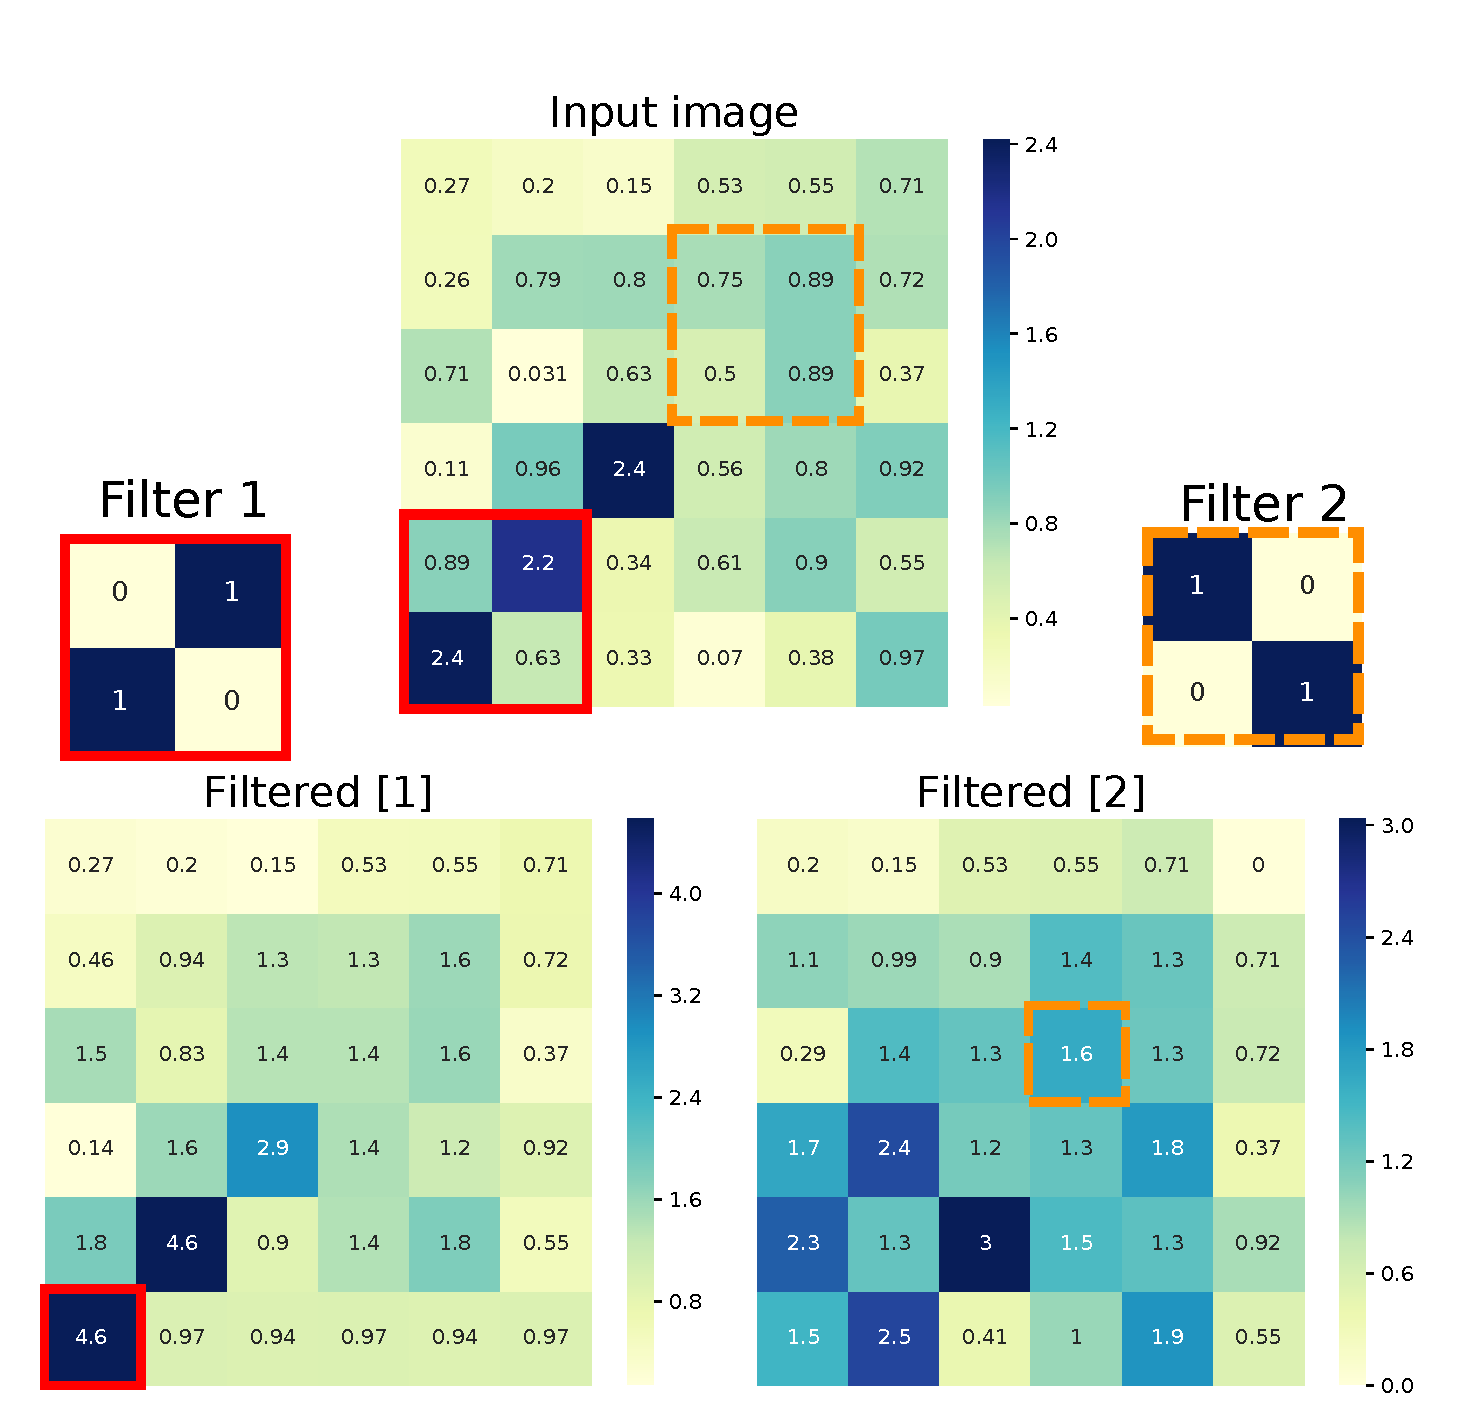
\includegraphics[width=\columnwidth]{C4_cnn/conv_filters.pdf}
    \caption{Convolutional filters can be designed to `pick out' certain features within an image. In this simple example above, the first filter (filter 1) matches the diagonal line in the bottom left of the input better than filter 2. The output filtered image the exaggerates this filter. The coefficients of the filter i.e. $F_{m,n}$ in Eq.~\ref{machine:cnn:conv:equation}, in this are set to ones and zeros.
    These are the weights which are trained by the network. In this an cases that follow, to get the same size image in the output as the input, the image is padded with zeros. I this image it was necessary to pad above and to the right of the image. The output of a convolutional layer is then the filtered images above after a bias and activation function have been applied. }
    \label{machine:cnn:convlayer:input}

\end{figure}

A convolutional layer has a number of different hyper-parameters which can be varied when setting up a model.
Below I list each of the adaptable parameters and what they do.

\begin{description}
\item[Filter size] The filter size is the size and shape of the convolutional filter. In Fig.~\ref{machine:cnn:convlayer:input} we use a filter size of 2$\times$2. The filter does not have to be square, however must be less than the dimensions of the image.

\item[Number of filters] The number of filters can be any value. If you have $K$ filter kernels, then the convolutional layer will output $K$ filtered images. In Fig.~\ref{machine:cnn:convlayer:input} we use two filters and therefore, the output of the layer is two images.

\item[Activation function] The activation function is generally kept the same for each of the layers, however this can be set here. The different types have been explained in Sec.~\ref{machine:nn:activation} and are applied as in Eq.~\ref{machine:cnn:conv:equation}.

\item[Stride] A normal convolutional layer applies a filter by multiplying by a filter, then shifting over by one pixel and repeating. Applying a stride mean rather than shifting by one pixel, one shifts by a number greater than one. This reduces the size of the output by the same factor of stride. i.e. if you skip one pixel (a stride of 2) then the image will be half the size on output. This has a similar affect to max-pooling which we describe in Sec.~\ref{machine:cnn:maxpool} an use for the rest of this work.  
\end{description}

The convolutional layers with reduce the number of updatable parameters used in each network or model.
However, the output of a convolutional layer is a number of images which ar potential the same size as the input. 
This has potentially increased the size of the parameter space for the next layer.
To decrease this a type of layer known as max-pooling is used.

%%%%%%%%%
%%%%%%%%
\subsection{\label{machine:cnn:maxpool}Max pooling layers}
%%%%%%%%%%%%
%%%%%%%%%%%

Max pooling layers are designed to reduce the size of the problem whilst holding on to as much important information as possible.
These do not contain any trainable parameters.
The idea of this layer is relatively simple, it reduces the image size by taking the maximum value in a region of a given size.
Fig.~\ref{machine:cnn:maxpool:image} shows the output of the first filtered image in Fig.~\ref{machine:cnn:convlayer:input}.
The image is then reduced by a 2$\times$2 max pooling layer.
The output of max-pooling Then shows a large value in the bottom left, this is where the input image matched the filter in Fig.~\ref{machine:cnn:convlayer:input}.
This demonstrates how the max-pooling layer can hold on to important information whilst reducing the image size.

\begin{figure}[h]
    \centering
    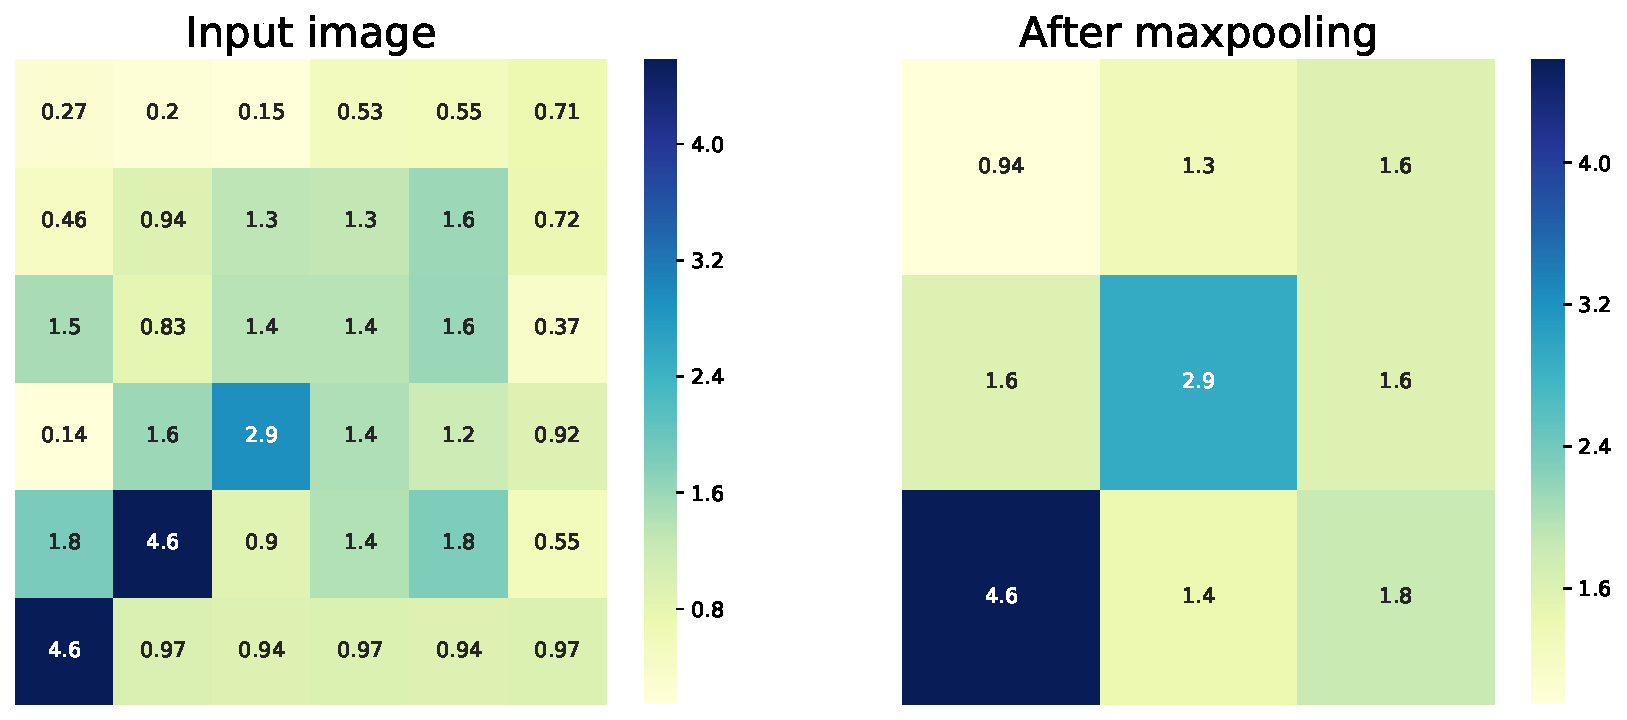
\includegraphics[width=\columnwidth]{C4_cnn/maxpool.pdf}
    \caption{Max pooling layers aim to reduce the size of am image whilst retaining important information within the original image. Above shows an example where a 2$\times$2 max-pooling layer is used on the output of Filter 1 in Fig.~\ref{machine:cnn:convlayer:input}. This retains the information that the input image matches the filter in the bottom left.}n
    \label{machine:cnn:maxpool:image}
\end{figure}

%%%%%%%%%%%%%
%%%%%%%%%%%%%%
\subsection{CNN structure}
%%%%%%%%%%%%%%
%%%%%%%%%%%%%%

\glspl{CNN} are usually structured such that they can extract larger features from an input image, then the outputs from this are passed on to be classified.
The `feature extraction' part of the network consists of the convolutional layers and the max-pooling described in Sec.~\ref{machine:cnn}.
The outputs of the final max-pooling layer are then flattened and used as the input to a fully connected network.
This fully connected network the classifies these outputs into a number of classes.
Fig.~\ref{machine:cnn:structure:example} shows an example of the layout. 
Here an input image which is the same as in previous examples is passed onto a single convolutional layer with two different filters.
The output of two filtered images is passed to a max-pooling layer.
The two max-pooled images are flattened into 18 input neurons, this then passes through a fully connected network to a single output neuron.
This shows a simple example, however, there are many hyper-parameters of the network which can be changed.
These include: the number of filters in a convolutional layer, the number of convolutional layers and max-pooling layers, the number of hidden layers in the fully connected section and the number of neurons in the hidden layers. 
This example also shows the network being classified to a single output as this is how we use \glspl{CNN} for the following work.

\begin{sidewaysfigure}[hp]
	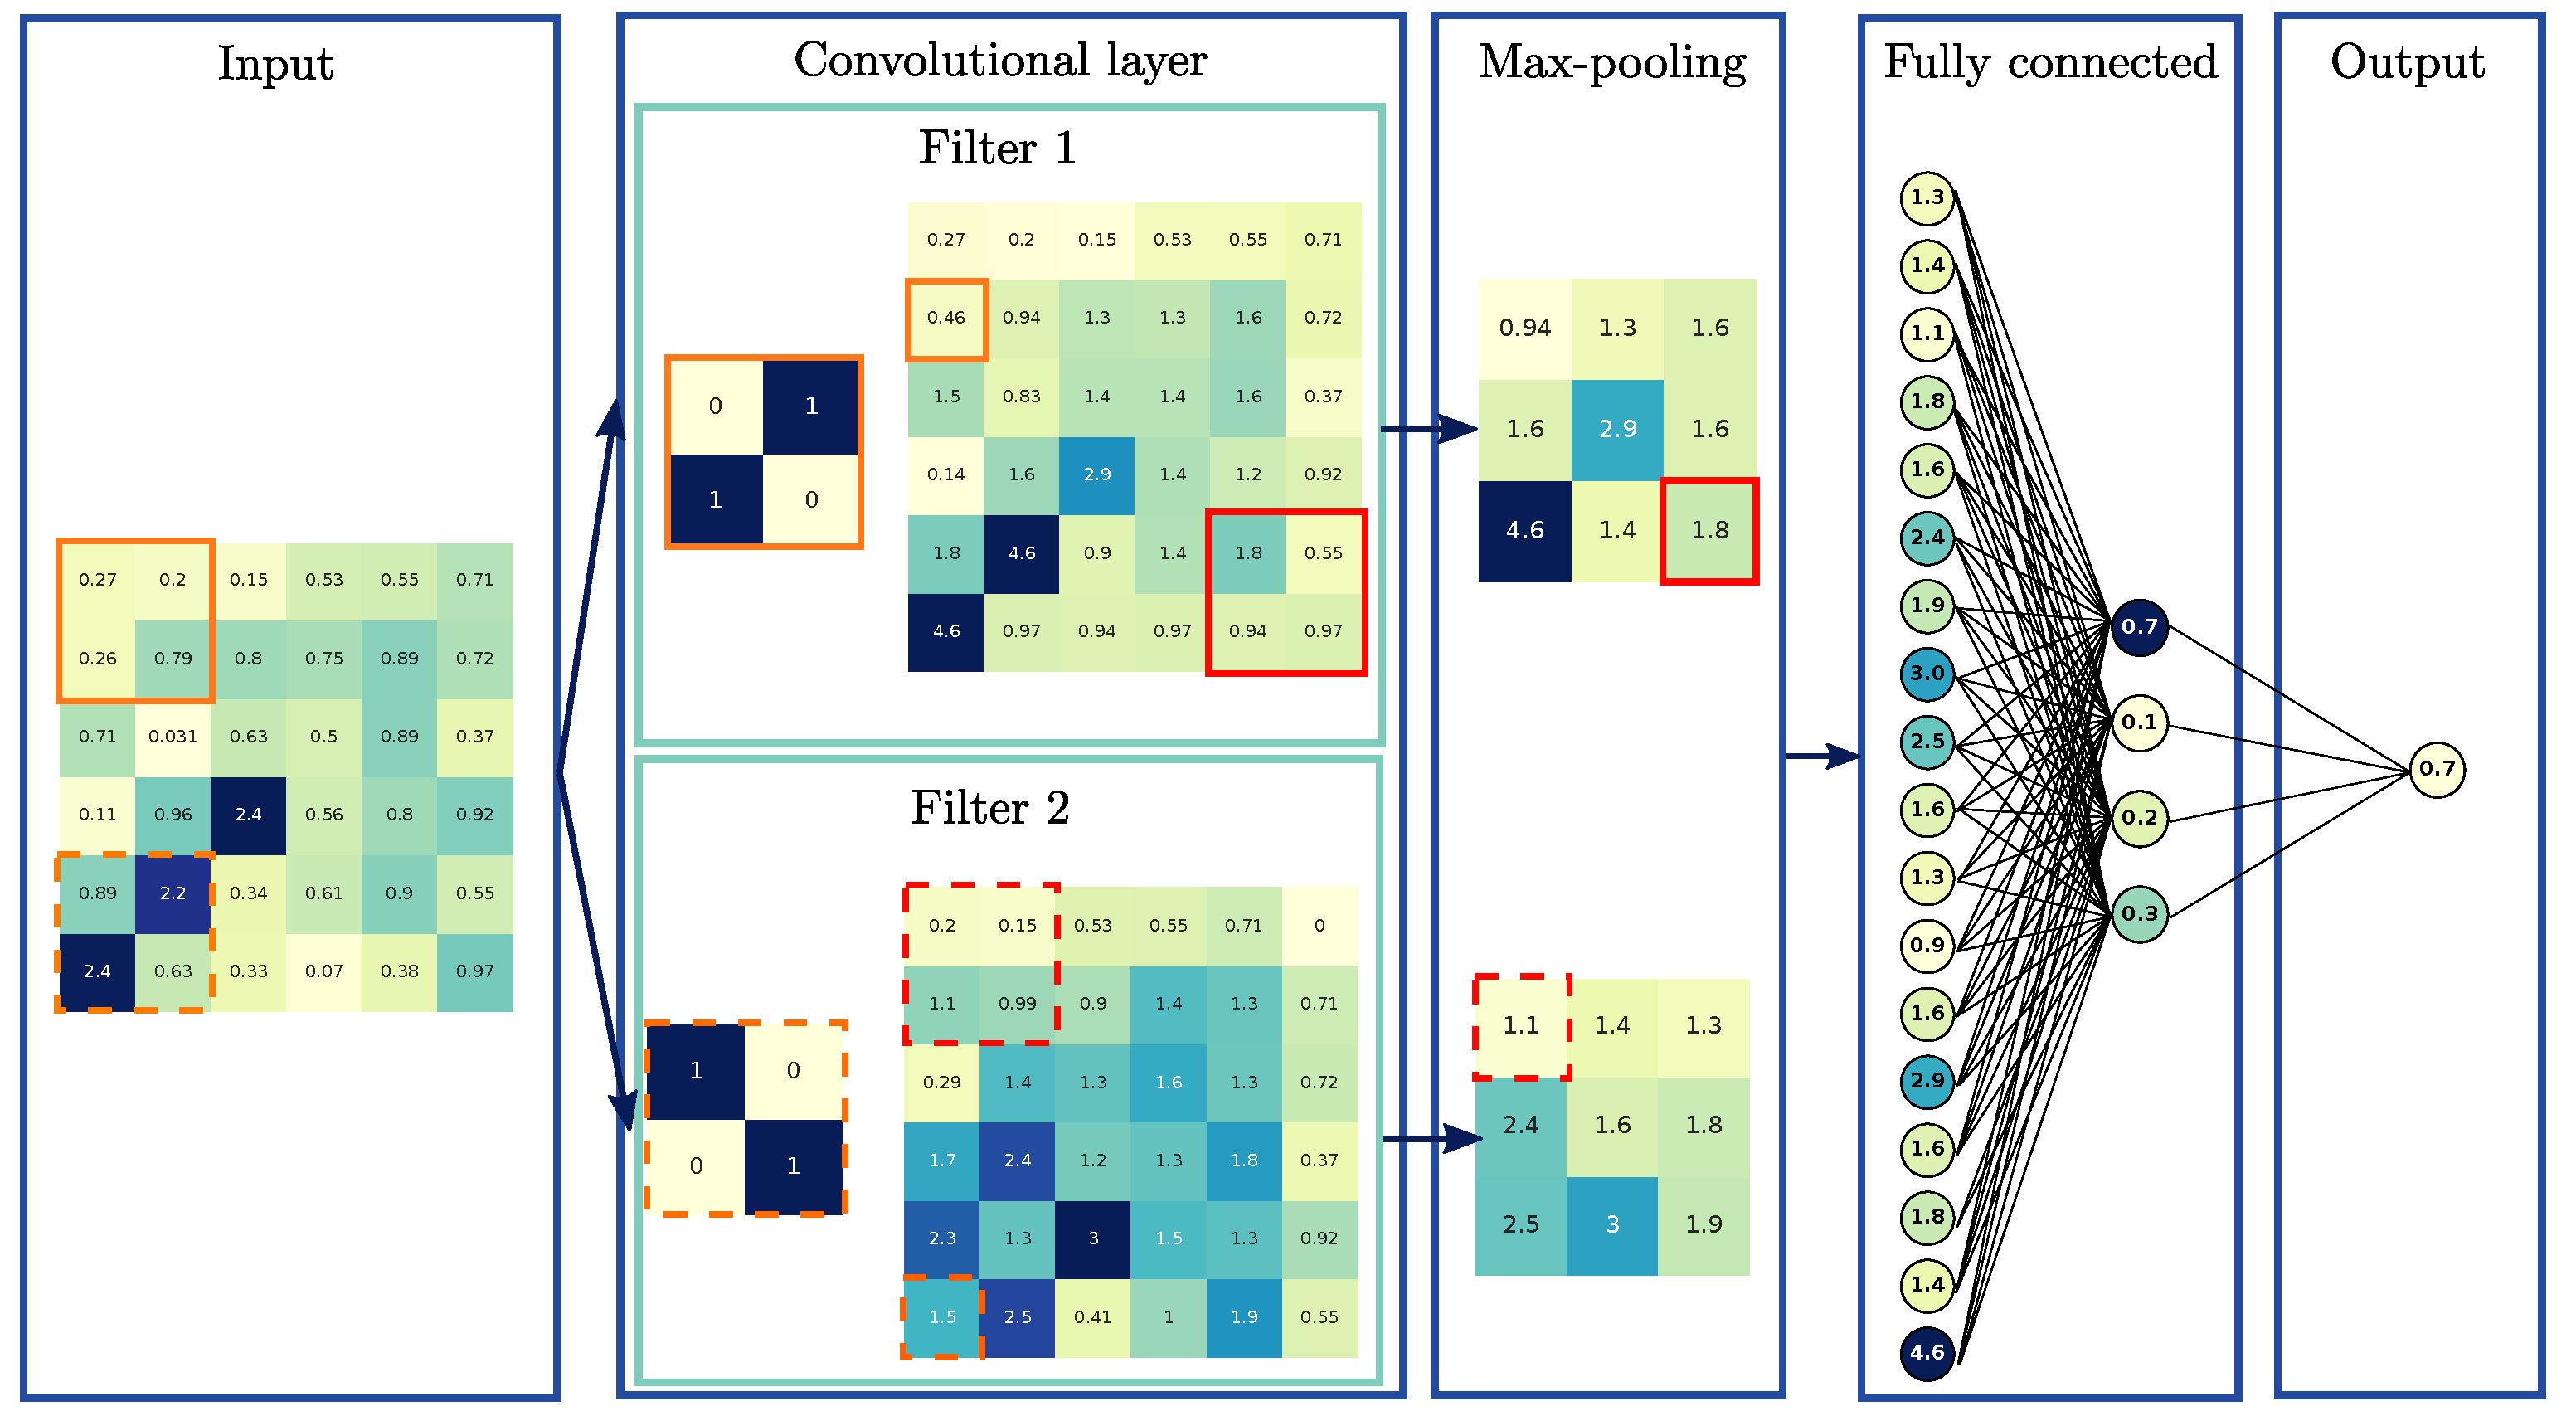
\includegraphics[width=\textwidth]{C4_cnn/cnn_structure_ex.pdf}
	\caption{Convolutional neural networks consist of two broad sections, the `feature extraction' part which is the convolutional and max-pooling layers, and the classification part which is the fully connected part of the network. This diagram shows a simple example of an image passing through a single convolutional layer with two filters, a single max-pooling layer and a simple fully connected network with a single hidden layer consisting of 4 neurons. The values in this diagram omit the use of any activation function such that the values are easier to follow. In a real network the activation functions are important.}
	\label{machine:cnn:structure:example}
\end{sidewaysfigure}


%%%%%%%%%%%%%%%%%
\section{\label{machine:training}Training}
%%%%%%%%%%%%%%%%%

% introduce training concept
%
Once the structure of the network is decided, the network needs to be trained.
This means that the weights and bias' for every neuron and filter need to be updated such
that the neural network gives a useful output. For this
work we will classify input time-frequency spectrograms into a signal or noise class using a single output neuron.
This neuron outputs a value in the range [0,1] by using a sigmoid activation function.
In our case the \gls{CNN} is trained using a process called supervised learning. 
In supervised learning, the class of each input example is know. For example, we assign a label of 1 when the
input is a time-frequency spectrogram which includes a simulated \gls{CW}
signal. Similarly a time-frequency spectrogram with no simulated signal is assigned a label of 0. 
In general when training neural networks this way, the performance of the network can be improved by increasing the number of input examples which are shown to the network.
This stops the network from over-fitting to specific examples. Instead it should generalise to the full input and learn the underlying features within the data.

\subsection{Loss function}

%Training procedure
%
Initially each of the training examples is propagated though the network to its single output value which lies between 0 and 1. Using a loss function, this output is then be compared to
the label of the input data which is either 0 or 1. There are many types of loss function which can be used, this depends on the type of problem which one wants to solve. As we are classifying
between two classes in out networks, the loss function, $L$, is the binary
crossentropy defined as,
%
\begin{equation}\label{cnn:loss} 
L = -\frac{1}{N} \sum_{i}^{N} y_i\log{(p_i)} + (1-y_i)\log{(1-p_i)},
\end{equation}
%
where $p$ is the networks predicted output which has any value in the range $[0,1]$ and $y$ is the true output which has binary labels 0 or 1. This is calculated as the sum over all training examples. 
The loss function is minimised when the output matches the `truth'. This essentially
tells the neural network how close to the truth it is. The weights and bias' of
the neural network can be updated based on the value of this loss function. The
process of updating the weights and other parameters is called back-propagation,
and typically uses a form of gradient descent
\cite{kingma2015AdamMethod}.
Back-propagation uses the derivative of the loss function with respect to a weight to update that weight.
If changing that weight in a particular direction decreases the loss function, then the weight will be updated in that direction.
The size of the change of the weight value is related to the change in the size loss function.
This means that the weights can be updated to minimise the loss function and therefore improve the performance of the network.

%%%
%%%
\subsection{Training procedure}
%%%
%%%

The training procedure entails passing a set of training examples through the network a number of times. 
Once the entire training data set has been passed through the network (forward pass) and the weights have been updated accordingly (back propagation), the training has completed one epoch.
If the data was passed and the weights were updated a single time, the loss may decrease by is likely not at a minimum.
Passing the data through again may move the weights to a lower loss.
This process is repeated a number of times to try and find the minimum loss.
When training there the value of the loss at each epoch is monitored, the trend of the loss of the training set should always decrease. 
In general  subset of the training data is set aside and not used in the training procedure, this is known as validation data. 
After each epoch the value of the loss for this validation set can be measured, i.e. all the validation data is passed though the network. 
This can be used to monitor the training of the network. If the validation loss begins to increase then this is a sign that the network is over-fitting to the training data-set.


%%%%%%%%%%%%%%%%%%%%%%%%%%%%%%%%%%%%%%%%%%%%%%
%%%%%%%%%%%%%%%%%%%%%%%%%%%%%%%%%%%%%%%%%%%%%%%%
\section{\label{machine:cw}Application to CW search}
%%%%%%%%%%%%%%%%%%%%%%%%%%%%%%%%%%%%%%%%%%%%%%%%%
%%%%%%%%%%%%%%%%%%%%%%%%%%%%%%%%%%%%%%%%%%%%%%%

The aim for this work is to use a \gls{CNN} to classify \gls{LIGO} data into one of two classes: signal or noise.
Here the signal class refers to a \gls{CW} signal from an isolated neutron star as described in Sec.~\ref{searchcw:model}.
Noise then refers to anything else which appear in the data, from Gaussian noise to instrumental artefacts. 
In Sec.~\ref{soap:results} to reduce the effect of instrumental artefacts, each of the search sub-bands was analysed by eye to determine if a sub-band was contaminated. 
Sub-bands which contained an artefact were then removed from the search.
This is a time consuming process. The main goal of the \gls{CNN} approach is to automate this part of the search.
This section will describe how we design the network to extract features and distinguish signals from instrumental artefacts.
We will then present results form searches in a range of \gls{LIGO} observing runs which include: S6, O1 and O2.


%%%%%%%%%%%%%%%
%%%%%%%%%%%%5%%
\subsection{\label{machine:cw:structure}Network structure}
%%%%%%%%%%%%%%%
%%%%%%%%%%%%%%%

In this section the structure of the networks which are used in this analysis
are described. There are three main inputs of data for each \gls{CNN}: spectrograms, Viterbi maps and the Viterbi statistic. Each of these are different representations of the raw detector data. In this analysis we train a separate \gls{CNN} for each of
these inputs and then a further three which use these combinations of inputs:
Viterbi map + spectrogram, Viterbi map + Viterbi statistic and Viterbi map +
Viterbi statistic + spectrogram. In all of the layers excluding the output layer of each \gls{CNN}, the activation functions in Eq.~\ref{machine:cnn:conv:equation} and \ref{machine:nn:neuron:equation} are defined by a function titled `leakyRELU' \cite{maas2013RectifierNonlinearities}. 
For our output neuron a sigmoid function is
used as an activation function such that the output is limited between 0 or 1.
For a given input a \gls{CNN} can then output a value between 0 and 1. When the output value is closer to 1, the input is more likely to contain a signal. 
The output value can then be treated as a detection statistic. 
The structure of the network is shown in Fig.~\ref{machine:results:cnnlayout} and is explained below. 

\begin{description}
	\item [Viterbi statistic] This is the simplest of the networks and will
	give the exact same result as the Viterbi statistic on its own. This is a
	single neuron which takes in the Viterbi statistic applies a weight and bias
	and then passes through a sigmoid function.
	
	\item [Viterbi map] The Viterbi map \gls{CNN} takes in a down-sampled Viterbi map of size (156,89), this is described more in Sec.~\ref{machine:data:downsample}.
	This \gls{CNN} consists of two convolutional layers and 3 fully connected layers. The first layer has
	8 filters which have a size of $5\times5$ pixels, the second layer has 8
	filters with a size of $3\times3$ pixels. After each of these layers we use a
	max-pooling layer with a size of $8\times8$ pixels. This then passed into three
	fully connected layers which all have 8 neurons and used leakyRELU activation
	functions. Finally these lead to an output neuron which uses a sigmoid
	function.
	
	\item [Spectrogram] The spectrogram \gls{CNN} takes in a down-sampled spectrograms of size (156,89), this is described more in Sec.~\ref{machine:data:downsample}.
	This \gls{CNN} has an identical structure as the Viterbi map \gls{CNN}, however, takes two channels as input. The two channels are the spectrograms of two different detectors.
	
\end{description}

The next three networks are constructed from combinations of the previous described \glspl{CNN}.

\begin{description}
	\item [Viterbi map and spectrogram] To combine the spectrogram and Viterbi map network, we remove the final output neuron and its 8 weights from each of the networks. 
	The outputs from each network is then 8 neurons. These can be combined to a single sigmoid neuron which has 16 new weights.
	
	\item [Viterbi map and Viterbi statistic] In this network we combine the
	Viterbi statistic with the Viterbi map. As before, this uses the pre-trained
	Viterbi map and Viterbi statistic \glspl{CNN}. The output sigmoid neuron and corresponding weights are removed from each network. 
	The 8 neurons from the Viterbi map network and the single neuron from the Viterbi statistic network are then combined to a single neuron with 9 new weights.
	
	\item [Viterbi map, Viterbi statistic and spectrogram] This combination takes all component \glspl{CNN} from above. As before the final sigmoid output and the corresponding weights from each network are removed.
	The 8 neurons from the Viterbi map and spectrograms \glspl{CNN} and the single neuron from the Viterbi statistic are then joined into a single output neuron with 17 new weights. 
	
\end{description}

When combining \glspl{CNN} we use a process called transfer
learning~\cite{prattDiscriminabilityBasedTransfer}. This uses the pre-trained weights of the networks as a starting point to continue training. 
In our examples we found that we could fix the weights inside the pre-trained networks and just train the final 16 output weights from the neurons as in Fig.~\ref{machine:results:cnnlayout}.
These combinations of networks were chosen as the different representations of the data should contain slightly different information on the input.
For example, the Viterbi statistic contains no information on the structure of the track in the data and the Viterbi maps lost some information about lines in the band.
The addition of the spectrograms aimed to include even more information about this piece of data. 
Where when each of these are combined, the \gls{CNN} should be able to pick to important information from each of these representations.

% plot of vitmap and spretrogram structure 
%
\begin{figure}[p]
	\centering
	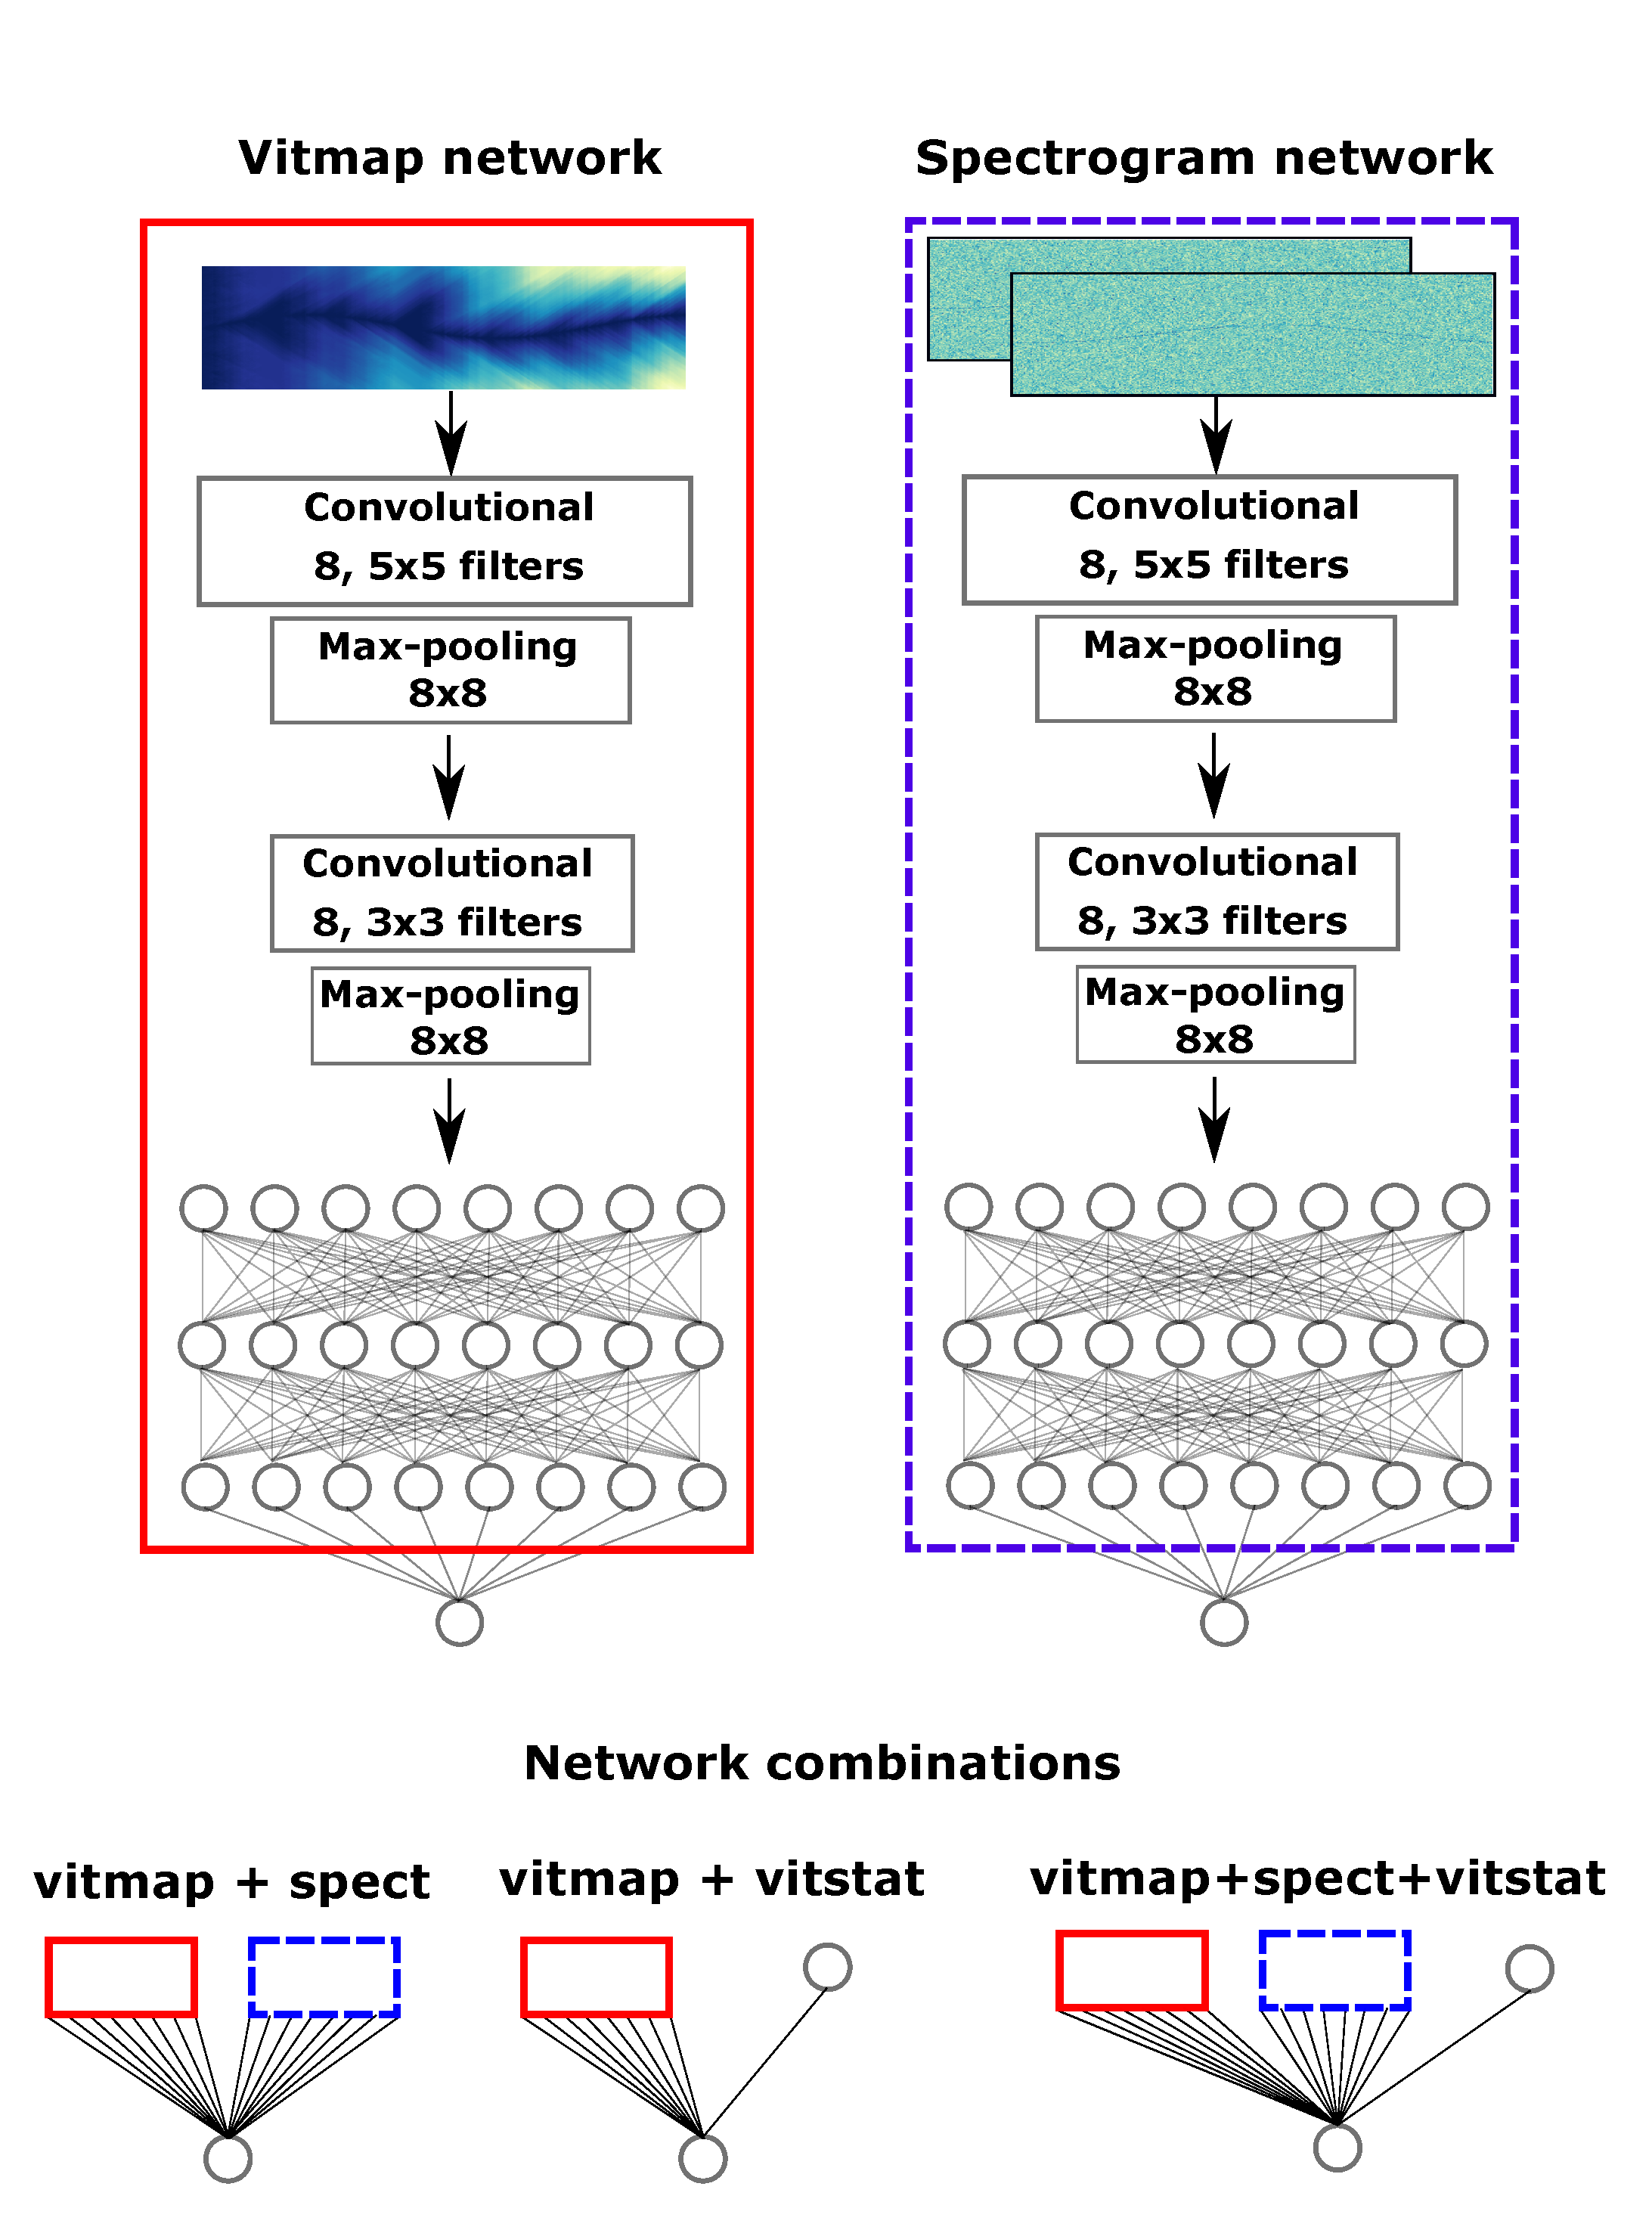
\includegraphics[width=0.9\columnwidth]{C4_cnn/networks.pdf}
	%
	\caption{\label{machine:results:cnnlayout} The structure of the Viterbi map and
		spectrogram \glspl{CNN} used in this analysis are the same, with the difference
		that the spectrogram takes two images as input. They each use two convolutional
		layers and 3 fully connected layers before they're output to a single neuron which represents the probability of belonging to the signal class. The
		Viterbi statistic network is a single neuron that transforms the statistic into
		a number between 0 and 1 representing the probability of belonging to
		the signal class. For the combinations of networks, we remove the final
		output neuron and its 8 weights, i.e. we take the part inside the red or blue box. The 8 outputs from each network are then combined to a single neuron with 16 new weights. }
	%
\end{figure}


%%%%%%%%%%%%%%%%%%%%%%%%%%%%%%%%%%%%%%
%%%%%%%%%%%%%%%%%%%%%%%%%%%%%%%%%%%%%%
\section{\label{machine:data} Data generation}
%%%%%%%%%%%%%%%%%%%%%%%%%%%%%%%%%%%%%%
%%%%%%%%%%%%%%%%%%%%%%%%%%%%%%%%%%%%%%

% define the 3 data types that we consider
%

To train the \glspl{CNN} we need to generate many examples of data, this include the three data products above: Time-frequency spectrograms, Viterbi maps and the Viterbi statistic. 
When a \gls{CNN} is trained it needs to see examples of all possible features which could appear in the data. This include, Gaussian noise, non-Gaussian artefacts and \gls{CW} signals. 
As non-Gaussian artefacts are difficult to simulate, it is possible to use the non-Gaussian artefacts in real data as part of the training set.
Therefore, for the majority of the analysis that follows, the time-frequency spectrograms which are used to generate the Viterbi data are from real detector data. The exact observing runs used will be explained in Sec.~\ref{results}. 

For the analysis that follows there are three main sets of data: training data,
test data and search data. 
Training data uses a set of augmented (see Sec.~\ref{data:augmentation}) time-frequency spectrograms containing simulated signals and is used to train each of
the networks. 
Test data is a separate set of simulations in time-frequency spectrograms which are not augmented. These are used to generate
efficiency curves and test the network.
Search data does not contain any simulated signal injections and is used to search for real signals within the data.

% describe the idea of odd and even bands
%
When training and testing a network it is important that the networks are not
trained and tested on the same data. Otherwise the \glspl{CNN} can learn specific
features of the training data and not the underlying
distribution of features. To avoid this, the spectrograms are split into $0.1$
Hz wide sub-bands where alternating bands are designated as `odd' or `even'.
This means that bands starting with 100.1,100.3 are odd and 100.2,100.4 are
even etc. The networks can then be trained on the odd bands and tested on the
even bands and vice versa.
This then means that each time we want to search over data, we will have two final networks. One which will be run on odd bands and a separately trained network which is run on even bands. 



%%%%%%%%%%%%%%%%%%%%%%%%%%%%%%%%%%%%%%%%%%%%%%%%%%%%%%%
\subsection{\label{machine:data:injections} Signal simulations}
%%%%%%%%%%%%%%%%%%%%%%%%%%%%%%%%%%%%%%%%%%%%%%%%%%%%%%%

% describe signal injection
%
To inject the simulated signals into real data we generate a random set of signal
parameters which are drawn from prior distributions defined in
Table~\ref{data:injections:table}. The \gls{SNR} of each simulation is then uniformly distributed between 50 and 150. Where the \gls{SNR} is the integrated `recovered' \gls{SNR}. This is calculated for each time segment using the definition of optimal \gls{SNR} in \cite{prix2007SearchContinuous}, the total \gls{SNR} is then the sum of the squares of these.
The \gls{GW} amplitude $h_{0}$ is scaled based on the noise \gls{PSD} to achieve this \gls{SNR}. 
The power spectrum of the signal can then be simulated in each time segment of a time-frequency spectrogram. This is done by assuming that the spectrogram is $\chi^2$ distributed.
The the antenna pattern functions are taken into account for the given source parameters and detector such that the \gls{SNR} for each time segment is calculated.
This \gls{SNR} is spread over neighboring frequency bins dependent on its location in frequency.
The power spectrum values can then be drawn from a non-central $\chi^2$ distribution with the non centrality parameter equal to the square of the \gls{SNR}.
Each signal is simulated in two detectors: \glspl{LIGO} H1 and L1.
The \glspl{SNR} reported below are then the sum of the squares of the \glspl{SNR} from each detector.



% Table for simulated signal priors
%
\begin{table*}
	%                                         
	\caption{\label{machine:data:injections:table} Table shows the upper and lower limits
		over which each signal parameter was randomized. The parameters $\alpha,\sin{\left(\delta \right)},f,\;\log{\left( \dot{f} \right)},\; \cos{\left(\iota
			\right)},\; \phi_0,\; \psi$ were sampled
		uniformly in the ranges specified in the table. The frequencies $f_{\rm l}$ and $f_{\rm u}$
		refer to the lower and upper frequency of the band that each signal is injected
		into. Excluding the distribution of frequencies $f$, all the injections parameters are sampled from the same distributions as the S6
		\gls{MDC}~\cite{walsh2016ComparisonMethods}.}
	%
	\scalebox{0.9}{
	\bgroup
	\def\arraystretch{1.5}
	\centering
	\begin{tabular}{c c c c c c c c r|}
		\hline
		\hline
		& $\alpha$ [rad]& $\sin\left(\delta \right)$ [rad] & $f$ [Hz]&
		$\log_{10}\left(\dot{f} [\rm{Hz/s}]\right)$ & $\cos{\iota}$ [rad]& $\phi$ [rad]& $\psi$ [rad]\\
		\hline
		lower bound & $0$ & $-1$ & $f_{\rm l} + 0.25$ & $-9$ & $-1$ & $0$ & $0$ \\
		\hline
		upper bound & $2\pi$ & $1$ & $f_{\rm u} - 0.25$ & $-16$ & $1$ & $2\pi$ & $\pi/2$ \\
		\hline
	\end{tabular}
	\egroup
}	
\end{table*}

%%%%%%%%%%%%%%%%%%%%%%%%%%%%%%%%%%%%%%%%%%%%%%%%%%%
\subsection{\label{machine:data:augmentation} Augmentation}
%%%%%%%%%%%%%%%%%%%%%%%%%%%%%%%%%%%%%%%%%%%%%%%%%%%

% introduce augmentation
%
To train a neural network, many examples of data from each class are needed to avoid over-fitting.
In our case when we use data between 40-500 Hz, splitting the data into 0.1 Hz wide sub-bands does not give enough data for the
networks to be trained effectively. Therefore, using a technique called data
augmentation~\cite{patrice1991TangentProp,baird1992DocumentImage} we can
artificially increase the number of training examples.
Augmentation is when data is transformed such that, to the network, it appears to be `new'
data. 
For example, by shifting a time-frequency band up and down in frequency, this appears to be a new realisation of noise which we can then inject a simulated signal into.
This would double the size of the training data-set and reduce the likelihood of over-fitting to the training data. 

% exactly what we do for augmentation
%
The augmentations are applied to the spectrograms from each of the detectors.
The augmentations that are used on each sub-band are: reversing the data in
time, flipping the data in frequency, rolling the data in time by a small
number of segments and shifting the data in frequency by a small number of
bins. As we use real data, there are gaps in time where the detectors were not
operating. We preserve the location of these gaps when augmenting the data.
When shifting the data in frequency, we shift each band up and down by 30 frequency bins (0.016 Hz) and up and down by 60 frequency bins (0.032 Hz).
When rolling the data in time, we roll each sub-band by 100 time segments (100 days). 
Fig.~\ref{machine:data:augmentation:examples} shows examples of the original data, a flip in frequency, a roll in time and a flip in time.
For each frequency shift, we flip the sub-band in time and frequency and roll the sub-band in time.
This then gives us 3 transformations for each of the 4 frequency shifts, which including the original data gives 20 times the number of training examples.

\begin{figure}
	\centering
	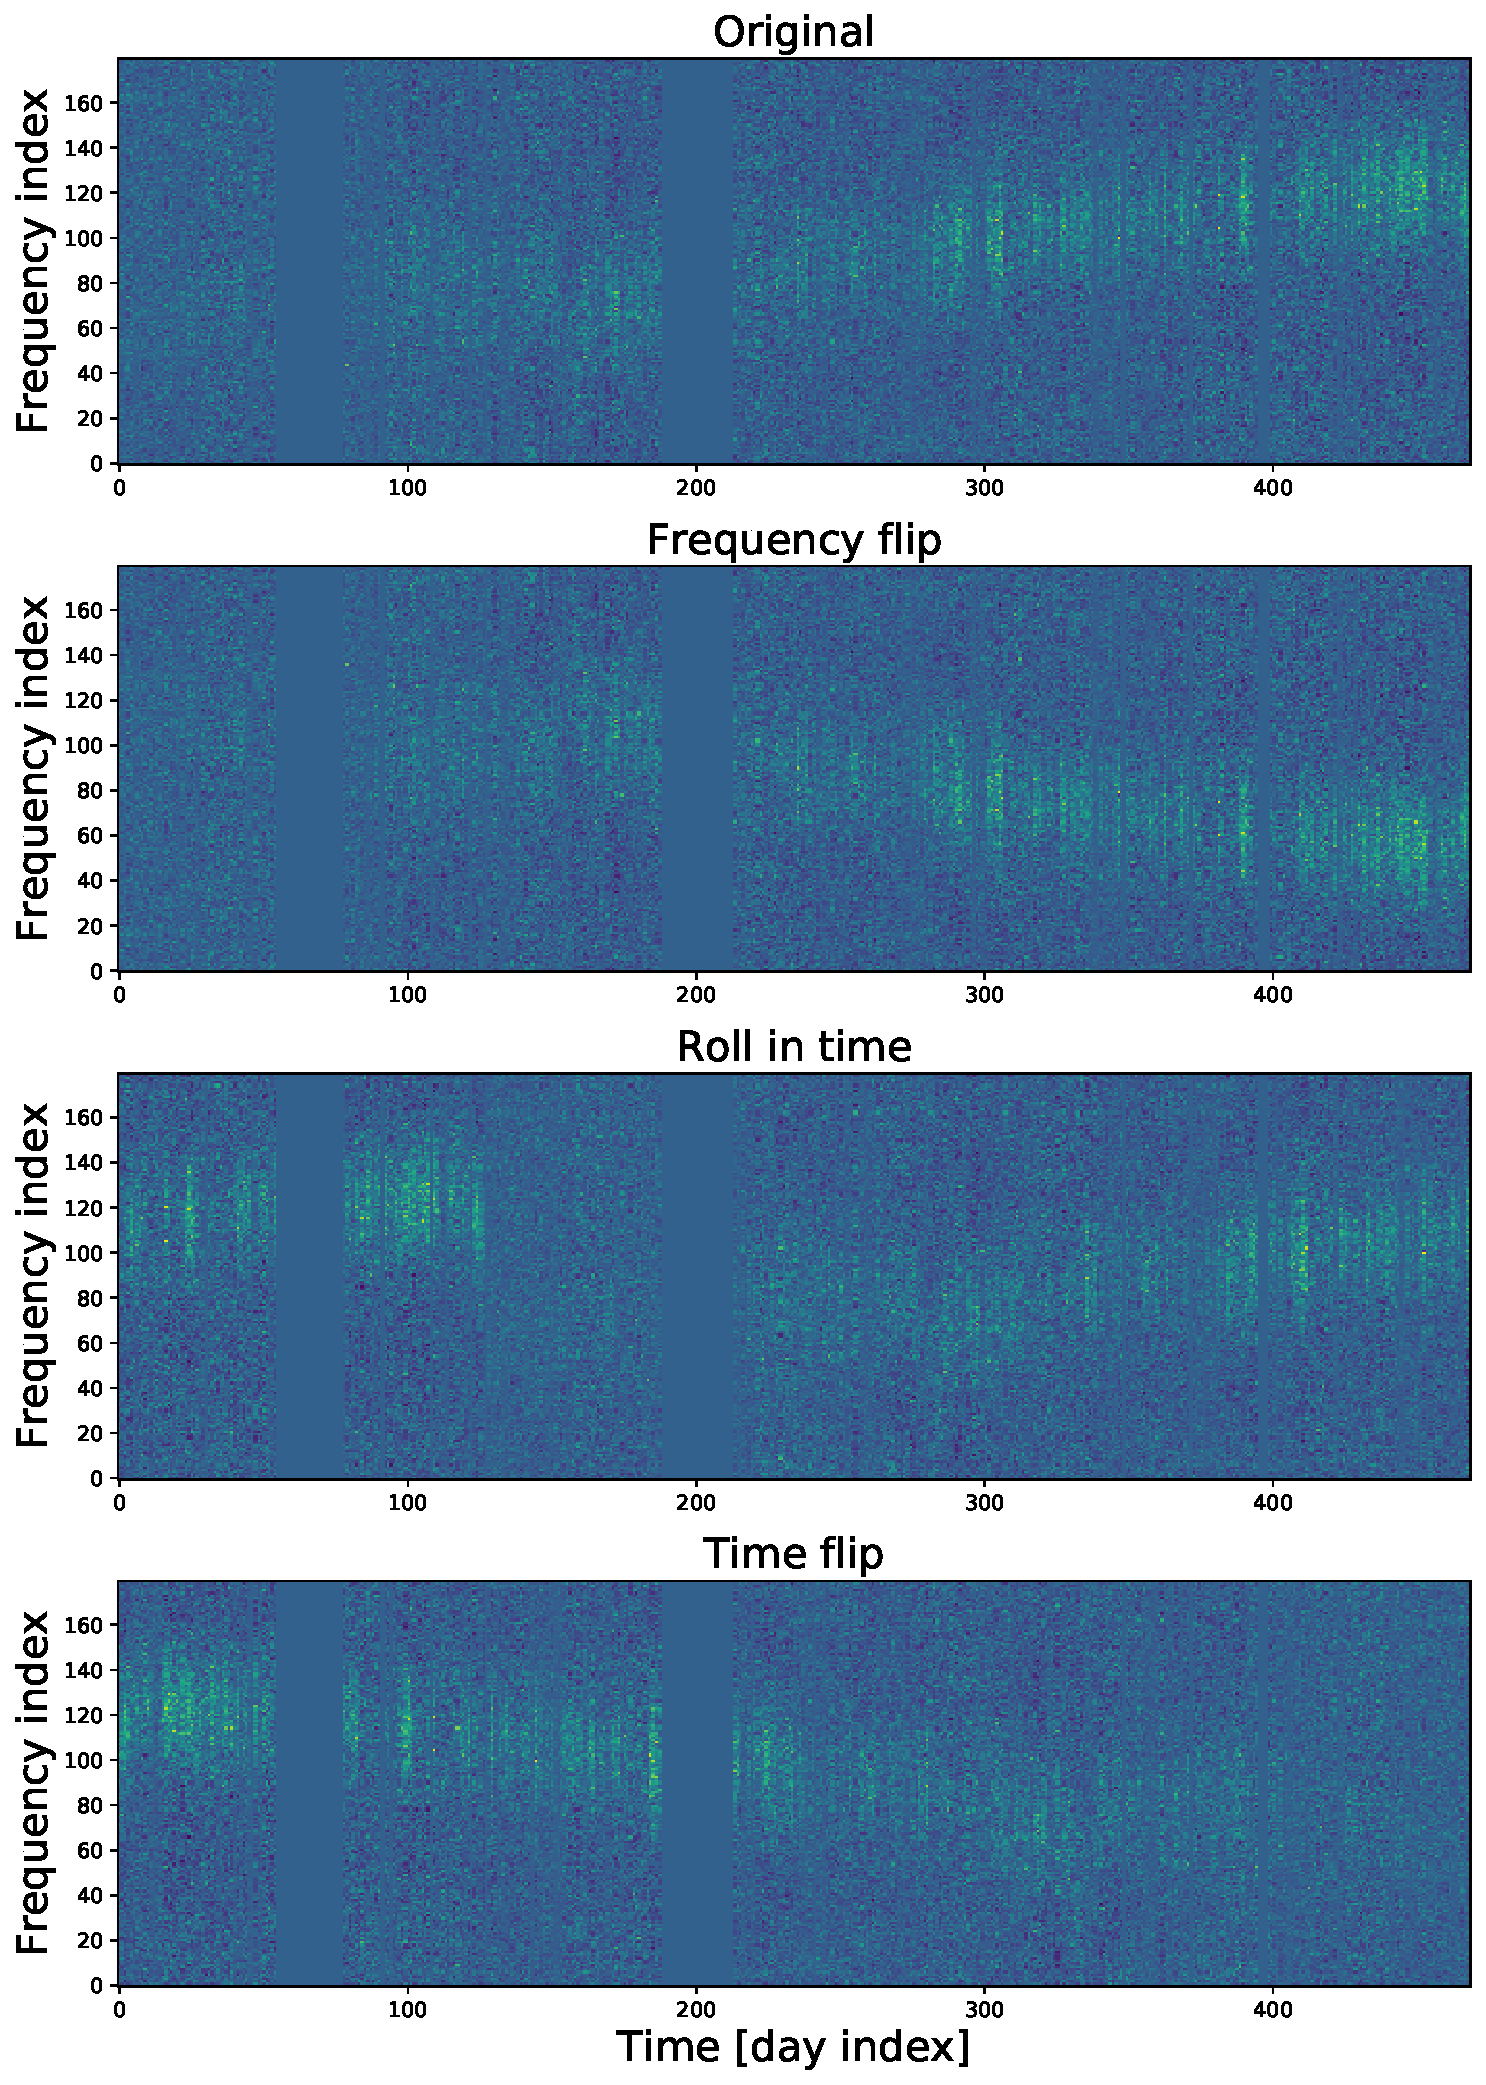
\includegraphics[width=0.8\columnwidth]{C4_cnn/augmentation.pdf}
	\caption{The data is transformed by flipping the data in frequency (panel 2),
		rolling the data in time by 100 bins (panel 3) and flipping the data in time
		(panel 4). The original summed spectrogram is show in panel 1. Simulated
		signals can then be injected using this data as noise. The plots above show a
		broad wandering line to demonstrate the changes to the data when it is
		augmented, however, the majority of sub-bands contain almost Gaussian
		noise.~\chris{I dislike figure titles. Could you use subfigures where they
			allow you to put a caption under each plot.} }
	\label{machine:data:augmentation:examples}
	
\end{figure}

%%%%%%%%%%%%%%%%%%%%%%%%%%%%%%%%%%%%%%%%%%%%%%%%%
\subsection{\label{machine:data:downsample} Downsampling}
%%%%%%%%%%%%%%%%%%%%%%%%%%%%%%%%%%%%%%%%%%%%%%%%%

% introduce downsampling
%
One further issue for our data sets are their size. The spectrograms we use have a large number of pixels within them.
This means that as the spectrograms are passed through the network, there are a large number of computations.
Both this number of computations and the memory requirements of the GPU mean that training a network with a large number of data points takes longer.
We implement a few methods to reduce the size of the data: summing time segments of
spectrograms and down-sampling these summed spectrograms.  

% describe the downsampling in time and frequency
%
The spectrograms are summed over one day, i.e., every 48 time segments, as
in~\cite{bayley2019SOAPGeneralised}. This should increase the \gls{SNR} for a
given signal within a given time-frequency bin assuming that the
signal remains within the frequency bin for the majority of the time segment.
To reduce the size of the data further, the package `resize' from scikit-image
\cite{vanderwalt2014ScikitimageImage} is used, this uses interpolation to
resize the summed spectrograms to a size of (156,89) [time segments,frequency
bins]. This size was defined based on the summed spectrograms of the S6 data-set. This is 1/3 the number of summed segments in time, 1/2 the number of segments in frequency. The down-sampling is applied to the
spectrograms and vitmap. 
In \cite{bayley2019SOAPGeneralised} we demonstrated that summing spectrograms can increase the speed and sensitivity of our search.
When down-sampling the image, we found that reducing the amount of data had a small affect on the sensitivity of the \glspl{CNN} used.

%%%%%%%%%%%%%%%%%%%%%%%%%%%%%
%%%%%%%%%%%%%%%%%%%%%%%%%%%%%
\section{\label{machine:pipeline}Search pipeline}
%%%%%%%%%%%%%%%%%%%%%%%%%%%%%%%%%%%%
%%%%%%%%%%%%%%%%%%%%%%%%%%%%%%%%%

% Introduce the plan for this section
%
In previous sections each component of the search pipeline has been described,
however, described below is how each component fits together.
Figure~\ref{machine:pipeline:flow} shows a flow diagram of the pipeline. The pipeline is
run in three different ways: training the \gls{CNN}, testing the search and
running a search on real data. 

% The flow diagram showing all the parts of the process
%
\begin{figure}[htp]
	\centering
	\scalebox{0.7}{
		

\tikzstyle{block} = [rectangle, draw, fill=blue!20, 
    text width=17em, text centered, rounded corners, minimum height=4em]
\tikzstyle{line} = [draw,line width=0.35mm, -latex']
\tikzstyle{fillnode} = [rectangle, fill=white, text centered]

\tikzstyle{blocktrain} = [rectangle, draw, fill=red!20, 
    text width=5em, text centered, rounded corners, minimum height=4em]
\tikzstyle{blocktest} = [rectangle, draw, fill=green!20, 
    text width=5em, text centered, rounded corners, minimum height=4em]
\tikzstyle{blocksearch} = [rectangle, draw, fill=black!5, 
    text width=5em, text centered, rounded corners, minimum height=4em]
\tikzstyle{blocktestbig} = [rectangle, draw, fill=green!20, 
    text width=17em, text centered, rounded corners, minimum height=4em]
\tikzstyle{blocksearchbig} = [rectangle, draw, fill=black!5, 
    text width=17em, text centered, rounded corners, minimum height=4em]
\tikzstyle{back group} = [fill=blue!20,rounded corners, draw=black!70, dashed, inner xsep=15pt, inner ysep=7pt, text centered]
\tikzstyle{back group1} = [fill=blue!20,rounded corners, draw=black!70, dashed, inner xsep=15pt, inner ysep=15pt, text centered]


\begin{tikzpicture}[node distance = 6em, auto]

    % Place node
    
  \node [block] (sft) {1.\\ SFTs from Time series};
  
  \node [block, below of=sft] (norm) {2. \\ Divide \ac{SFT} to running median and get power spectrum.};
  \node [block, below of=norm] (narrow) {3. \\ Narrowband \ac{SFT} };
  
  \node [block, below right =1.5cm and -0.9cm of narrow] (odd) {4. \\ Odd.};
  \node [block, below left =1.5cm and -0.9cm of narrow] (even) {4. \\ Even.};
  
  % odd blocks
    
  \node [blocktest,below of= odd] (testodd) {5b.\\ Test data};
  \node [blocktest, below of= testodd] (testsumodd) {6b. \\Test data};
  \node [blocktest, below of=testsumodd] (testlookupodd) {7b. \\ Test data};
  \node [blocktest, below of=testlookupodd] (testdownsampodd) {8b. \\  Test data};
  \node [below of= testdownsampodd](testblankodd) {};
    
  \node [blocktrain, left of= testodd] (trainodd) {5a.\\ Training data};
  \node [blocktrain, below of= trainodd] (trainsumodd) {6a. \\Training data};
  \node [blocktrain, below of=trainsumodd] (trainlookupodd) {7a. \\ Training data};
  \node [blocktrain, below of=trainlookupodd] (traindownsampodd) {8a. \\  Training data};
  \node [blocktrain, below of=traindownsampodd] (trainnetworkodd) {9. \\ Train `odd' \ \ac{CNN}};

  \node [blocksearch,right of=testodd] (searchodd) {5c.\\ Search data};
  \node [blocksearch, below of= searchodd] (searchsumodd) {6c. \\Search data};
  \node [blocksearch, below of=searchsumodd] (searchlookupodd) {7c. \\ Search data};
  \node [blocksearch, below of=searchlookupodd] (searchdownsampodd) {8c. \\  Search data};
  \node [below of= searchdownsampodd](searchblankodd) {};
  
  \node [blocktest, below = 1.4cm of testblankodd] (testclassifyodd) {10b.\\ Test data};
  \node [blocksearch, below = 1.4cm of searchblankodd] (searchclassifyodd) {10c.\\ Search data};

   
  % even blocks]
  
    \node [blocksearch,below of=even] (searcheven) {5c.\\ Search data};
  \node [blocksearch, below of= searcheven] (searchsumeven) {6c. \\Search data};
  \node [blocksearch, below of=searchsumeven] (searchlookupeven) {7c. \\ Search data};
  \node [blocksearch, below of=searchlookupeven] (searchdownsampeven) {8c. \\ Search data};
  \node [below of= searchdownsampeven](searchblankeven) {};
  
  \node [blocktest,left of= searcheven] (testeven) {5b.\\Test data};
  \node [blocktest, below of= testeven] (testsumeven) {6b. \\Test data};
  \node [blocktest, below of= testsumeven] (testlookupeven) {7b. \\Test data};
  \node [blocktest, below of=testlookupeven] (testdownsampeven) {8b. \\ Test data};
  \node [below of= testdownsampeven](testblankeven) {};
  
  \node [blocktrain, right of= searcheven] (traineven) {5a.\\ Training data};
  \node [blocktrain, below of= traineven] (trainsumeven) {6a. Training data};
  \node [blocktrain, below of=trainsumeven] (trainlookupeven) {7a. \\Training data};
  \node [blocktrain, below of=trainlookupeven] (traindownsampeven) {8a. \\ Training data};
  \node [blocktrain, below of=traindownsampeven] (trainnetworkeven) {9. \\ Train `even'  \ \ac{CNN}};

  
  \node [blocktest, below = 1.4cm of testblankeven] (testclassifyeven) {10b.\\ Test data};
  \node [blocksearch, below = 1.4cm of searchblankeven] (searchclassifyeven) {10c.\\ Search data};
  
% background blocks  
  
\begin{scope}[on background layer]
   
    \node (bkgen) [back group] [fit=(trainodd) (testodd) (searchodd) (traineven) (testeven) (searcheven) ] {5.\\Injections};
    
    \node (bksum) [back group] [fit=(trainsumodd) (testsumodd) (searchsumodd) (trainsumeven) (testsumeven) (searchsumeven)] {6.\\Sum spectrograms over \\1 day};
    
    \node (bksoap) [back group] [fit=(trainlookupodd) (testlookupodd) (searchlookupodd) (trainlookupeven) (testlookupeven) (searchlookupeven)] {7.\\Generate lookup tables \\and\\ run SOAP search.};
    
    \node (bkdown) [back group] [fit=(traindownsampodd) (testdownsampodd) (searchdownsampodd) (traindownsampeven) (testdownsampeven) (searchdownsampeven)] {8.\\Downsample spectrograms\\ and vitmaps.};
    
    \node (bkclassodd) [back group1] [fit=(testclassifyodd) (searchclassifyodd)] {};
     
    \node (bkclasseven) [back group1] [fit=(testclassifyeven) (searchclassifyeven)] {};

    
 \end{scope}
 
   % search and testing
  
  \node [blocktestbig, below right =1.1cm and -3.5cm of bkclasseven] (output) {11c.\\ Generate efficiency curves from test data.};
  \node [blocksearchbig, below left= 1.1cm and -3.5cm of bkclassodd] (outputsearch) {11a.\\ Take top 1\% of search bands for followup.};
  
  % Draw edges
  \path [line] (sft) -- (norm);
  \path [line] (norm) -- (narrow);
  
  % even lines
  
   \path [line] (narrow) -- (even);
  
  \path [line] (even) -- (testeven);
  \path [line] (even) -- (traineven);
  \path [line] (even) -- (searcheven);
  
  \path [line,red!60] (traineven) -- (trainsumeven.north);
  \path [line,green!60] (testeven.south) -- (testeven.south|-testsumeven.north);
  \path [line,black!60] (searcheven.south) -- (searcheven.south|-searchsumeven.north);
  
  \path [line,green!60] (testeven.south|-testsumeven.south) -- (testeven.south|-testlookupeven.north);
  \path [line,red!60] (traineven.south|-trainsumeven.south) -- (traineven.south|-trainlookupeven.north);
  \path [line,black!60] (searcheven.south|-searchsumeven.south) -- (searcheven.south|-searchlookupeven.north);
  
  \path [line,green!60] (testeven.south|-testlookupeven.south) -- (testeven.south|-testdownsampeven.north);
  \path [line,red!60] (traineven.south|-trainlookupeven.south) -- (traineven.south|-traindownsampeven.north);
  \path [line,black!60] (searcheven.south|-searchlookupeven.south) -- (searcheven.south|-searchdownsampeven.north);
  
  \path [line,red!60] (traindownsampeven) -- (trainnetworkeven);
  \path [line,green!60] (testdownsampeven) -- (testclassifyeven);
  \path [line,black!60] (searchdownsampeven) -- (searchclassifyeven);
  
  %\path [line,black!60] (searcheven.south|-searchdownsampeven.south) -- (searcheven.south|-classifyeven.north);
  %\path [line,green!60] (testeven.south|-testdownsampeven.south) -- (testeven.south|-classifyeven.north);
  
  \path [line,red!60] (trainnetworkeven) -- (bkclassodd);
  
  %% odd lines
  
   \path [line] (narrow) -- (odd);
  
  \path [line] (odd) -- (testodd);
  \path [line] (odd) -- (trainodd);
  \path [line] (odd) -- (searchodd);
  
  \path [line,red!60] (trainodd) -- (trainsumodd.north);
  \path [line,green!60] (testodd.south) -- (testodd.south|-testsumodd.north);
  \path [line,black!60] (searchodd.south) -- (searchodd.south|-searchsumodd.north);
  
  \path [line,green!60] (testodd.south|-testsumodd.south) -- (testodd.south|-testlookupodd.north);
  \path [line,red!60] (trainodd.south|-trainsumodd.south) -- (trainodd.south|-trainlookupodd.north);
  \path [line,black!60] (searchodd.south|-searchsumodd.south) -- (searchodd.south|-searchlookupodd.north);
  
  \path [line,green!60] (testodd.south|-testlookupodd.south) -- (testodd.south|-testdownsampodd.north);
  \path [line,red!60] (trainodd.south|-trainlookupodd.south) -- (trainodd.south|-traindownsampodd.north);
  \path [line,black!60] (searchodd.south|-searchlookupodd.south) -- (searchodd.south|-searchdownsampodd.north);
  
  \path [line,red!60] (traindownsampodd) -- (trainnetworkodd);
  \path [line,green!60] (testdownsampodd) -- (testclassifyodd);
  \path [line,black!60] (searchdownsampodd) -- (searchclassifyodd);
  
  %\path [line,black!60] (searchodd.south|-searchdownsampodd.south) -- (searchodd.south|-classifyodd.north);
  \%path [line,green!60] (testodd.south|-downsampodd.south) -- (testodd.south|-classifyodd.north);
  
  \path [line,red!60] (trainnetworkodd) -- (bkclasseven);
  
  % search and test
  
  \path [line,green!60] (testclassifyeven) -- (output);
  \path [line,black!60] (searchclassifyeven) -- (outputsearch);
  
  \path [line,green!60] (testclassifyodd) -- (output);
  \path [line,black!60] (searchclassifyodd) -- (outputsearch);
  
  % final labels over lines
  
   \node[fillnode,below] at (bkclasseven.south) {Classify sub-bands with \ `odd' \ac{CNN}};
   
   \node[fillnode,below] at (bkclassodd.south) {Classify sub-bands with \ `even' \ac{CNN}};
 
    
\end{tikzpicture}}
	\caption{\label{machine:pipeline:flow} This diagram shows the SOAP pipeline from start to finish. There are three main sections: Training (red), Testing (green) and Searching (grey) for both the odd and even bands. The blue sections mean that the same operations is done in all cases.}
	
\end{figure}

% describe the elements of the flow diagram
%
\begin{description}
	%    
	\item[1. SFTs] Generate 1800s long \glspl{SFT} from detector time-series
	data. \glspl{SFT} of this length are a standard set for \gls{CW} searches which are continuously generated during observing runs by members of the \gls{LIGO} collaboration. 
	%   
	\item[2. Normalising] The \glspl{SFT} are then divided by their running median with a window width of 100 frequency bins.
	If we assume the resulting \glspl{SFT} to be $\chi^2$ distributed, we can apply a correction factor using LALSuite code {\tt XLALSFTtoRngmed} \cite{ligoscientificcollaboration2018LIGOAlgorithm} such that their power spectrum has a mean of $\sim 1$. 
	By then multiplying this by 2, the noise like parts of the spectrum are $\chi^2$ distribution with two degrees of freedom.
	
	%
	\item[3. Narrowbanding] The computational efficiency can be improved if the data is split into narrow bands.
	This is because the analysis can be completed on each band in parallel on separate CPU nodes. 
	In this search the spectrograms are split into $2.1$ Hz wide bands every $2$ Hz, i.e.
	100.0-102.1, 102.0-104.1 etc. The bands are $2.1$ Hz wide as the analysis on each node will further split the data into 0.1 Hz wide sub-bands. 
	The overlap then allows the sub-band from 1.95-2.05 to be calculated on a node.
	This band size was chosen based on the available
	computational memory at the time. 
	%    
	\item[4. Band splitting] A \gls{CNN} should not be trained on the same
	data that it will be tested on.
	For this reason, each of the $0.1$ Hz wide sub-bands are split
	into `odd' or `even' bands. A \gls{CNN} can then be trained on even bands and tested on odd bands and vice versa.
	%
	\item[5a. Training data generation] To generate training data the process is
	the same as described in Sec.~\ref{data}. Each of the $0.1$ Hz sub-bands is
	`augmented' as in Sec.~\ref{machine:data:augmentation}. For each of the augmented
	bands, the data is duplicated such that there is a second copy of every augmented band. 
	In the copied set of bands, signals are injected into them with
	\glspl{SNR} in the range 50-150. This gives us and example for a noise class and
	a signal class. There are two of these sets, one for `even' bands and
	one for `odd'.
	%
	\item[5b. Test data generation] For test data, signals following the parameters in
	Tab.~\ref{machine:data:injections:table} are injected in to 50\% of the $0.1$ Hz
	sub-bands. These signal have and \gls{SNR} in the range 20-200. The \gls{SNR} range here is wider than the training set as a method to test how the trained networks perform s on a wider range od \glspl{SNR}. Here we again have a
	set for `odd' and a set for `even'.
	%    
	\item[5c. Search data] This data is generated such that we can search for a
	real signal. The sub-bands described in part 4 are now overlapping by 0.05 Hz.
	This means that if there is an astrophysical signal it should be fully contained within at
	least one sub-band. We do assume that a signals frequency does not drift by more than 0.1 Hz, which is assumed to be true for isolated neutrons stars $< 500$ Hz.  There are both `odd' and `even' versions of this search data.
	%
	\item[6. Summing spectrogram] As in~\cite{bayley2019SOAPGeneralised} the
	spectrograms are summed over one day, i.e., every 48 time segments (1 day) of
	the spectrogram are summed. This is done separately for each of the 6 data-sets
	(3 for `odd', 3 for `even'). 
	%     
	\item[7. Generate lookup tables and run SOAP search] Before the SOAP search is
	run, the line-aware statistic lookup tables need to be generated as
	in~\cite{bayley2019SOAPGeneralised}. Then for each of the 6 data-sets (3 for
	`odd', 3 for `even') the SOAP search is run separately. 
	%     
	\item[8. Down-sample data] At this stage there are four elements which are
	saved for each of the 6 data-sets. The two spectrograms, the Viterbi maps and
	the Viterbi statistic. The spectrograms and the Viterbi maps are down-sampled
	to a size of ($156\times 89$) using interpolation from scikit-image's
	resize~\cite{vanderwalt2014ScikitimageImage}. This size was chosen based on the
	S6 \gls{MDC} data-set, where this is 1/3 the length in time and 1/2 the width in
	frequency of the summed spectrograms. 
	This was chosen such that the \glspl{CNN} trained efficiently and still achieved a reasonable sensitivity. 
	%
	\item[9. Train Networks] The down-sampled training data is then used to train a
	\glspl{CNN}. One \gls{CNN} is trained on `odd' bands and a different \gls{CNN} with
	the same structure is trained on `even' bands. 
	%
	\item[10b. Run search on test data] The trained \glspl{CNN} from part 9 are then
	used to classify each sub-band in the test data with injections, this returns a
	statistic on the range $[0,1]$. The close the value is to 1 the more likely it is from an astrophysical signal, therefore,  the statistic can be interpreted as an estimate of the probability of a signal being present. Here the \gls{CNN}
	trained on the `odd' bands is tested using the `even' bands and vice
	versa. The algorithms are run on this test data to asses the sensitivity of the analysis.
	%
	\item[10c. Run search on real data] The trained \glspl{CNN} from part 9 are then
	used to classify each sub-band in the search data, this returns a statistic in
	$[0,1]$. This statistic is the same as in part 10b. 
	Once again the \gls{CNN} trained on the `odd' bands is tested using
	the `even' bands and vice versa.
	%        
	\item[11a. Signal candidates] The signals which have a statistic in the top
	1\% can be taken as potential candidates. 
	This can then potentially be followed up with other \gls{CW} search methods. 
	%    
	\item[11c. Efficiency curves] The output statistics from the test data-set (11b.) can
	be plotted against \gls{SNR} to see how the network classified signals with the
	\gls{SNR} of the injection. This can potentially be extended to other signal parameters also. 
	Then the efficiency curves can be generated, this is described in further detail in Sec.~\ref{machine:results:sensitivity}.
	
	\chris{One thing I am still confused about is search, test and training data.
		Maybe I missed it but can you point me to the place (or add text to explain)
		that the search data is just the data, the training data is a mix of augmented
		data and injections, and so is the test data. In all cases the data is real.
		The injections in the test data are different to the ones in the training data
		and the augmentations in the test data is different to the training data.} \joe{this is said at the start of the data section \ref{data}}
	
\end{description}





%%%%%%%%%%%%%%%%%%%%%%%%%%%%
%%%%%%%%%%%%%%%%%%%%%%%%%%%%
\section{\label{machine:results}Results}
%%%%%%%%%%%%%%%%%%%%%%%%%%%%
%%%%%%%%%%%%%%%%%%%%%%%%%%%%

% a general introduction statement about the results
%
The networks described in Sec.~\ref{machine:cw:structure} were trained and tested on four different data-sets: the S6 \gls{MDC} as in~\cite{bayley2019SOAPGeneralised,walsh2016ComparisonMethods}, our own
injections into O2 data, Gaussian noise which had the same gaps and noise
floor as the S6 data-set, and our own injections into real S6 data. Each of
the searches use training and test data in the frequency range of 100-400 Hz,
except the S6 \gls{MDC} which uses data in the range 40-500 Hz for testing and
training. 


\subsection{\label{machine:results:sensitivity} Sensitivity}


% define the figures of merit - the depth and SNR
%
To investigate the sensitivity of the pipeline we use two measures: the
sensitivity depth $\mathcal{D}$ \cite{prix2007SearchContinuous} and optimal
\gls{SNR} $\rho$ \cite{behnke2015PostprocessingMethods} which are both defined
in \cite{bayley2019SOAPGeneralised} as,
%
\begin{equation}
\label{machine:results:depth}
\mathcal{D}(f) = \frac{\sqrt{S_h(f)}}{h_0},
\end{equation}
%
where $S_h(f)$ is the single-sided noise \gls{PSD} and $h_0$ is the \gls{GW}
amplitude. The optimal \gls{SNR} is defined as,
%
\begin{equation}
\rho^2 = \sum_X 4
\Re\int^{\infty}_{0}\frac{\tilde{h}^X(f)\tilde{h}^{X*}(f)}{S^X(f)}df,
\end{equation}
%
where $X$ indexes the detectors and $\tilde{h}(f)$ is the Fourier transform of
the time series of the signal $h(t)$. This expression is defined
in~\cite{prix2007SearchContinuous} for a double-sided \gls{PSD} and we have
defined it for the more common single-sided case.


% describe setting a false alarm threshold
%
The sensitivity curves shown in Fig.~\ref{machine:results:o2},\ref{machine:results:s6gauss} and
\ref{machine:results:s6mdc} were generated using a $1\%$ false alarm rate, where the
false alarm threshold is the value of our statistic where $1\%$ of sub-bands which
do not contain an injection exceed that value. This is then used as a detection
threshold.
The efficiency is defined as the fraction of events which exceed the false alarm rate for any given \gls{SNR}.
As the \gls{SNR} is sampled uniformly between the range 20-200 as in Sec.~\ref{machine:pipeline}, the efficiency cannot be calculated for any individual \gls{SNR}.
Instead, one can define some window around a point in \gls{SNR} and count the fraction of statistics which exceed the false alarm threshold within that window.
We define the window as a Gaussian with a standard deviation of 2, this is wide enough to contain enough injections per \gls{SNR} to achieve a reliable value. The Gaussian window was chosen to down weights statistics which are further away from the given point in \gls{SNR}.
This can then slide along the \gls{SNR} axes and estimate the efficiency as a function of \gls{SNR}
The efficiency curves $y$ are then be calculated using,
%
\begin{equation}
y(x) = \frac{\sum_i H(O_i - O^{1\%}) \mathcal{G}(x_i - x,2)}{\sum_i \mathcal{G}(x_i - x,2)},
\end{equation}
%
where $O_i$ is the output statistic from the \gls{CNN}, $O^{1\%}$ is the statistic value at a 1\% false alarm rate, $H$ is the Heaviside step function which has a value of 1 for positive values and 0 for negative values. $x_i$ is the \gls{SNR} of a simulation with output $O_i$, $x$ is the current location in \gls{SNR} and $\mathcal{G}(x_i - x,2)$ is a Gaussian with a
mean of the current \gls{SNR} and a standard deviation of 2.  
The sensitivity curves for each of the described data-sets are shown in
Figs.~\ref{machine:results:o2}, \ref{machine:results:o1}, \ref{machine:results:s6gauss} and
\ref{machine:results:s6mdc}.


%%%%%%%%
\subsubsection{O1}
%%%%%%%%%%

For the first test, injections were made into the O1 data-set as in Sec.~\ref{machine:data} between 100 Hz and 400 Hz. Then each of the 6 networks described in Sec.~\ref{machine:cnn:structure} were trained and tested on this data. 
Fig.~\ref{machine:results:o1} shows the sensitivity curves for this test for both \gls{SNR} and sensitivity depth for each of the 6 networks. Focusing on Fig.~\ref{machine:results:snr_o1}, the least sensitive, i.e. furthest to the right, of the \glspl{CNN} is the Viterbi statistic (vitstat), this is expected as we know that the Viterbi statistic is sensitive to instrumental lines. 
The spectrogram \gls{CNN} has an improved sensitivity over the Viterbi statistic, this importantly does not involve the SOAP search but is run entirely on down-sampled and summed spectrograms. 
Whilst this network is approaching the most sensitive of the examples in Fig.~\ref{machine:results:o1}, and with further efforts may reach it, this network takes $\sim10$ times the amount of training time. This will be explained in more detail in Sec.~\ref{machine:results:timing}.
The remaining networks achieved almost the same sensitivity. 
The vitmap network however, is the fastest of these to train and is used as an input for all of these remaining networks.
For the O1 data-set we show that with a false alarm of 1\% the Viterbi map \gls{CNN} achieves a sensitivity of SNR $~73$ and sensitivity depth of $~12\; {\rm Hz}^{-1/2}$ with 95\% efficiency.
The \gls{SNR} here should not be compared between different runs as this is the integrated `Recovered' \gls{SNR}. Therefore, observing runs, such as O1, which were shorted will appear to have a greater sensitivity when they in fact do not. 

\begin{figure}
	%\centering
	\begin{subfigure}[h]{0.5\textwidth}
		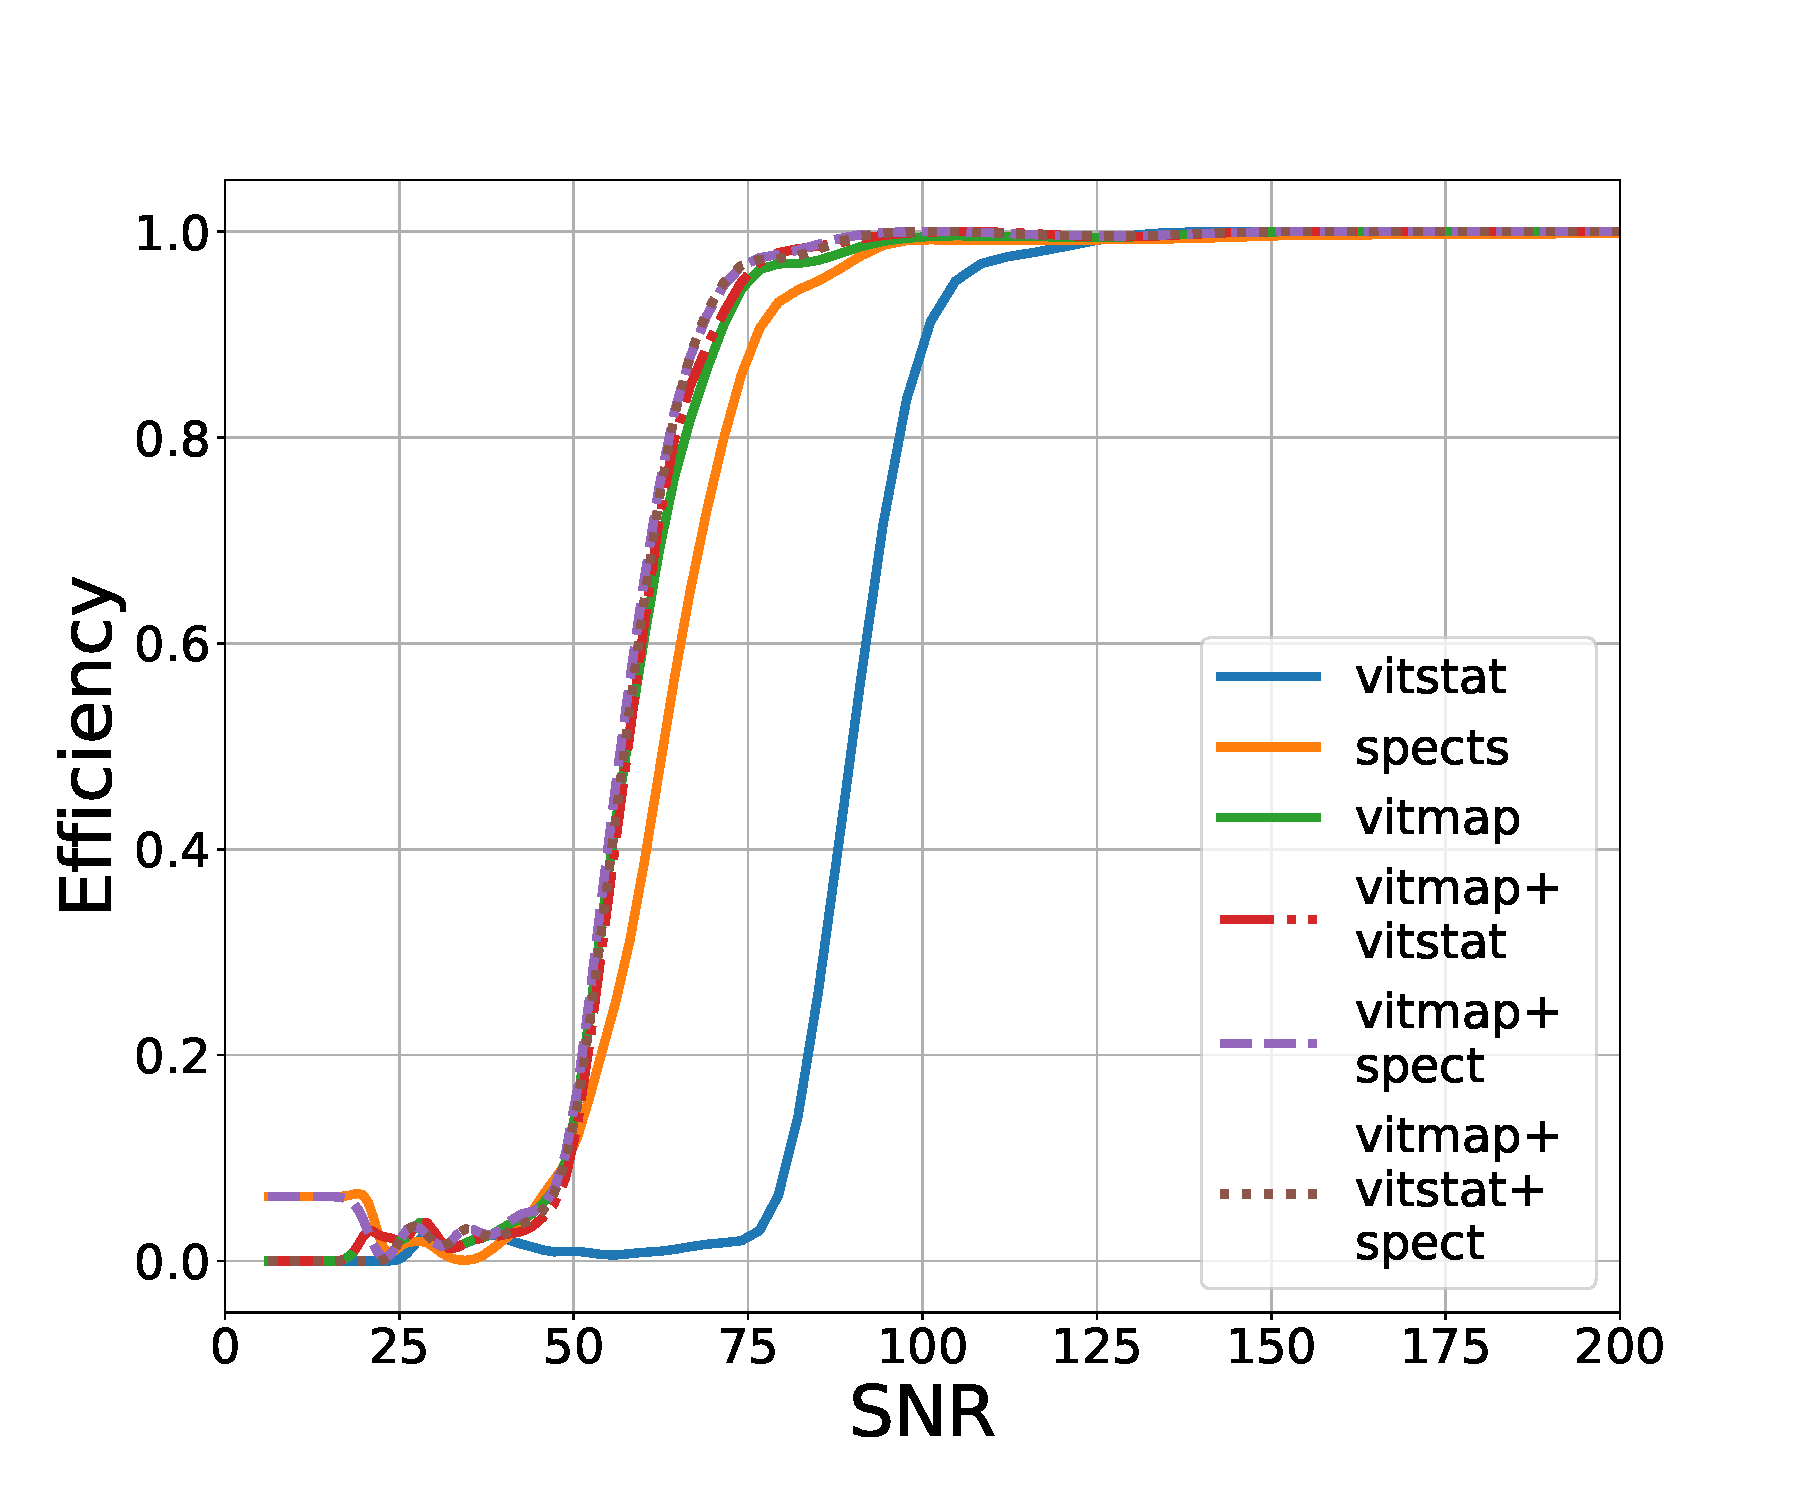
\includegraphics[width=\columnwidth]{C4_cnn/o1_snr_eff.pdf}
		\caption{\label{machine:results:snr_o1}}
	\end{subfigure}
	\begin{subfigure}[h]{0.5\textwidth}
		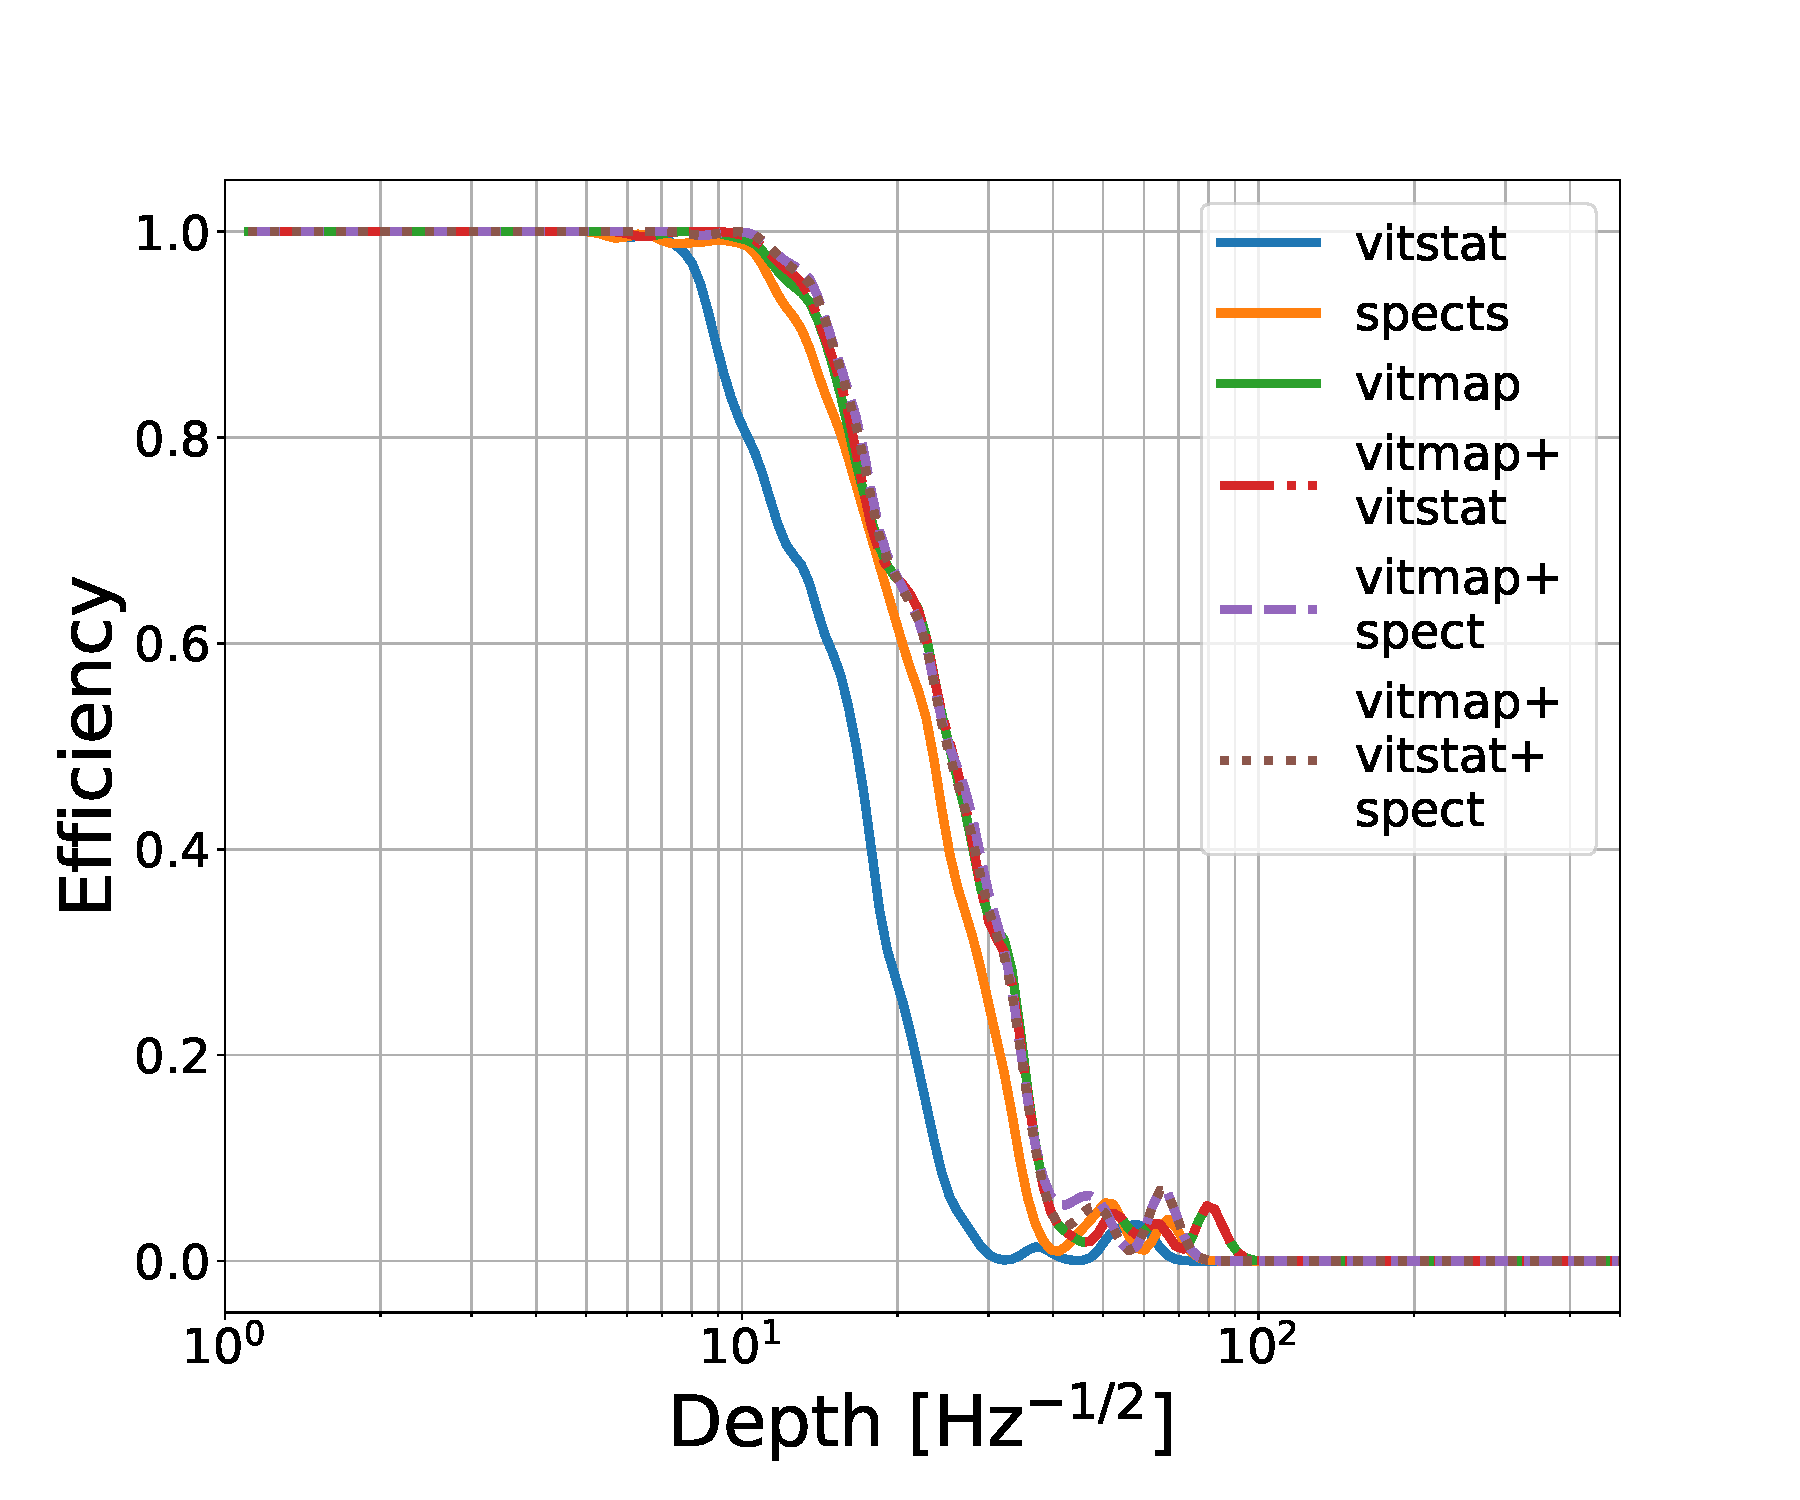
\includegraphics[width=\columnwidth]{C4_cnn/o1_depth_eff.pdf}
		\caption{}
		\label{machine:results:depth_o1}
	\end{subfigure}
	\caption{ In the O1 data-set, each of the six \glspl{CNN} were tested. The efficiency plots above are for a 1\% false alarm rate. }
	\label{machine:results:o1}
	
\end{figure}

%%%%%%%%%
\subsubsection{O2}
%%%%%%%%%%

For the next test, injections were made into the O2 data-set in the same way as in the last section. Then each of the 6 networks described in Sec.~\ref{machine:cw:structure} were trained and tested on this data. 
Fig.~\ref{machine:results:o2} shows the sensitivity curves for this test for both \gls{SNR} and sensitivity depth for each of the 6 networks.
The results here are very similar to the results from the O1 simulations.
The Viterbi statistic is the least sensitive `network', followed by the spectrogram \gls{CNN}.
The remaining four networks all achieve a similar sensitivity, each of these remaining networks contain the Viterbi map as one of their inputs. Therefore, it is assumed that the dominating effect on the sensitivity originated from the Viterbi maps. In following tests the focus will be with the Viterbi map \gls{CNN} as in all cases this is among the most sensitive.
For the O2 data-set we show that with a false alarm of 1\% the Viterbi map \gls{CNN} achieves a sensitivity of SNR $~95$ and sensitivity depth of $~12\; {\rm Hz}^{-1/2}$ with 95\% efficiency.
This result in the sensitivity depth in Fig.~\ref{machine:results:depth_o2} does not vary much from the results from O1, Fig.~\ref{machine:results:depth_o1}. 
Whilst one might expect the sensitivity to increase due to the increase in sensitivity and longer observing run.
However, this is not the case \joe{why?}.

\begin{figure}
	%\centering
	\begin{subfigure}[h]{0.5\textwidth}
		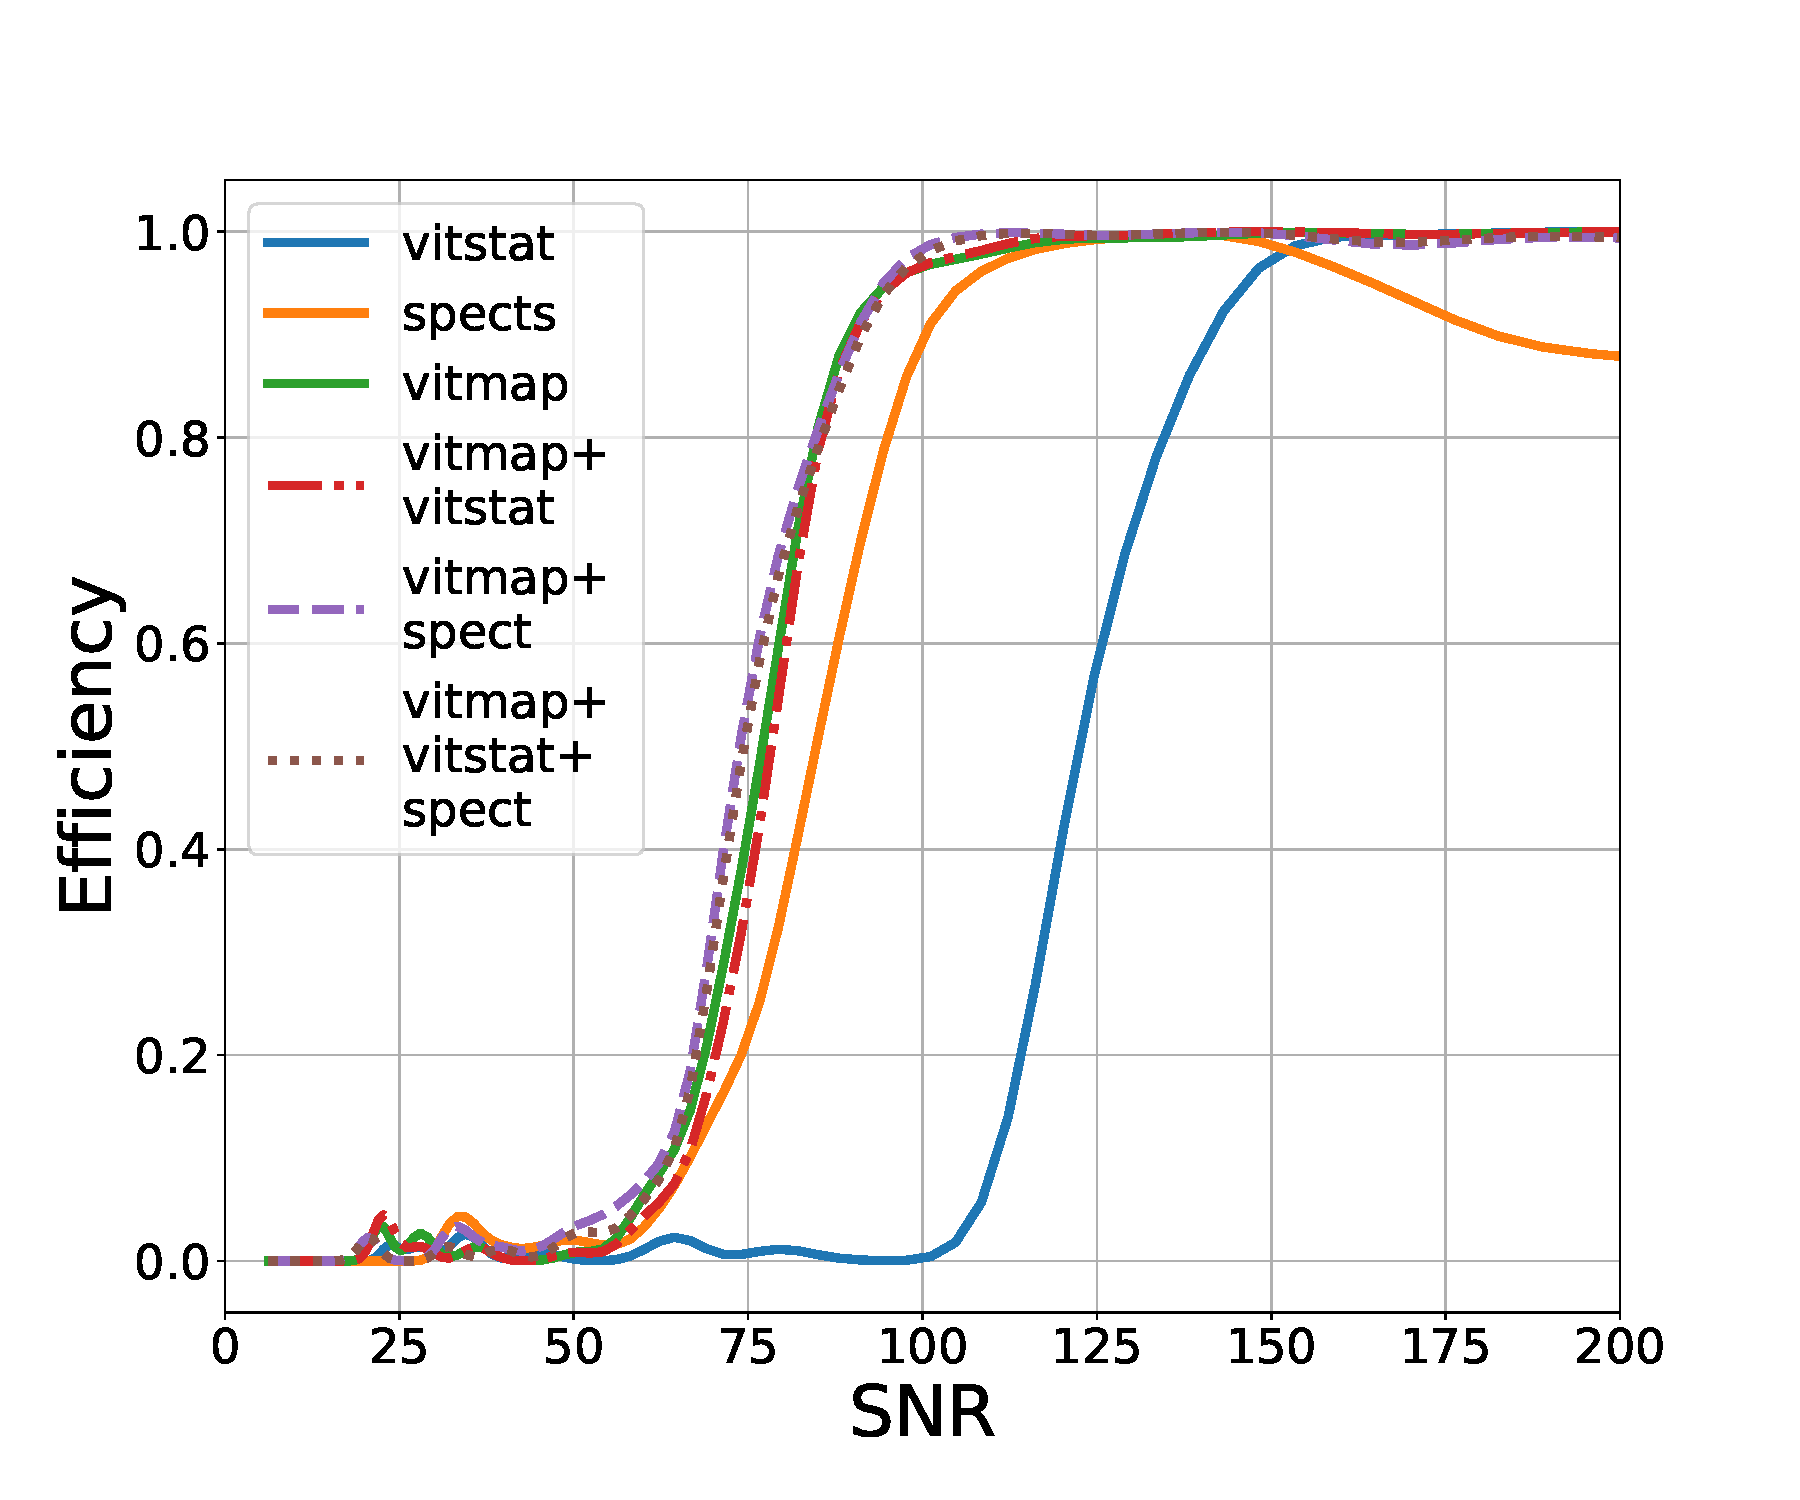
\includegraphics[width=\columnwidth]{C4_cnn/o2_snr_eff.pdf}
		\caption{}
		\label{machine:results:snr_o2}
	\end{subfigure}
	\begin{subfigure}[h]{0.5\textwidth}
		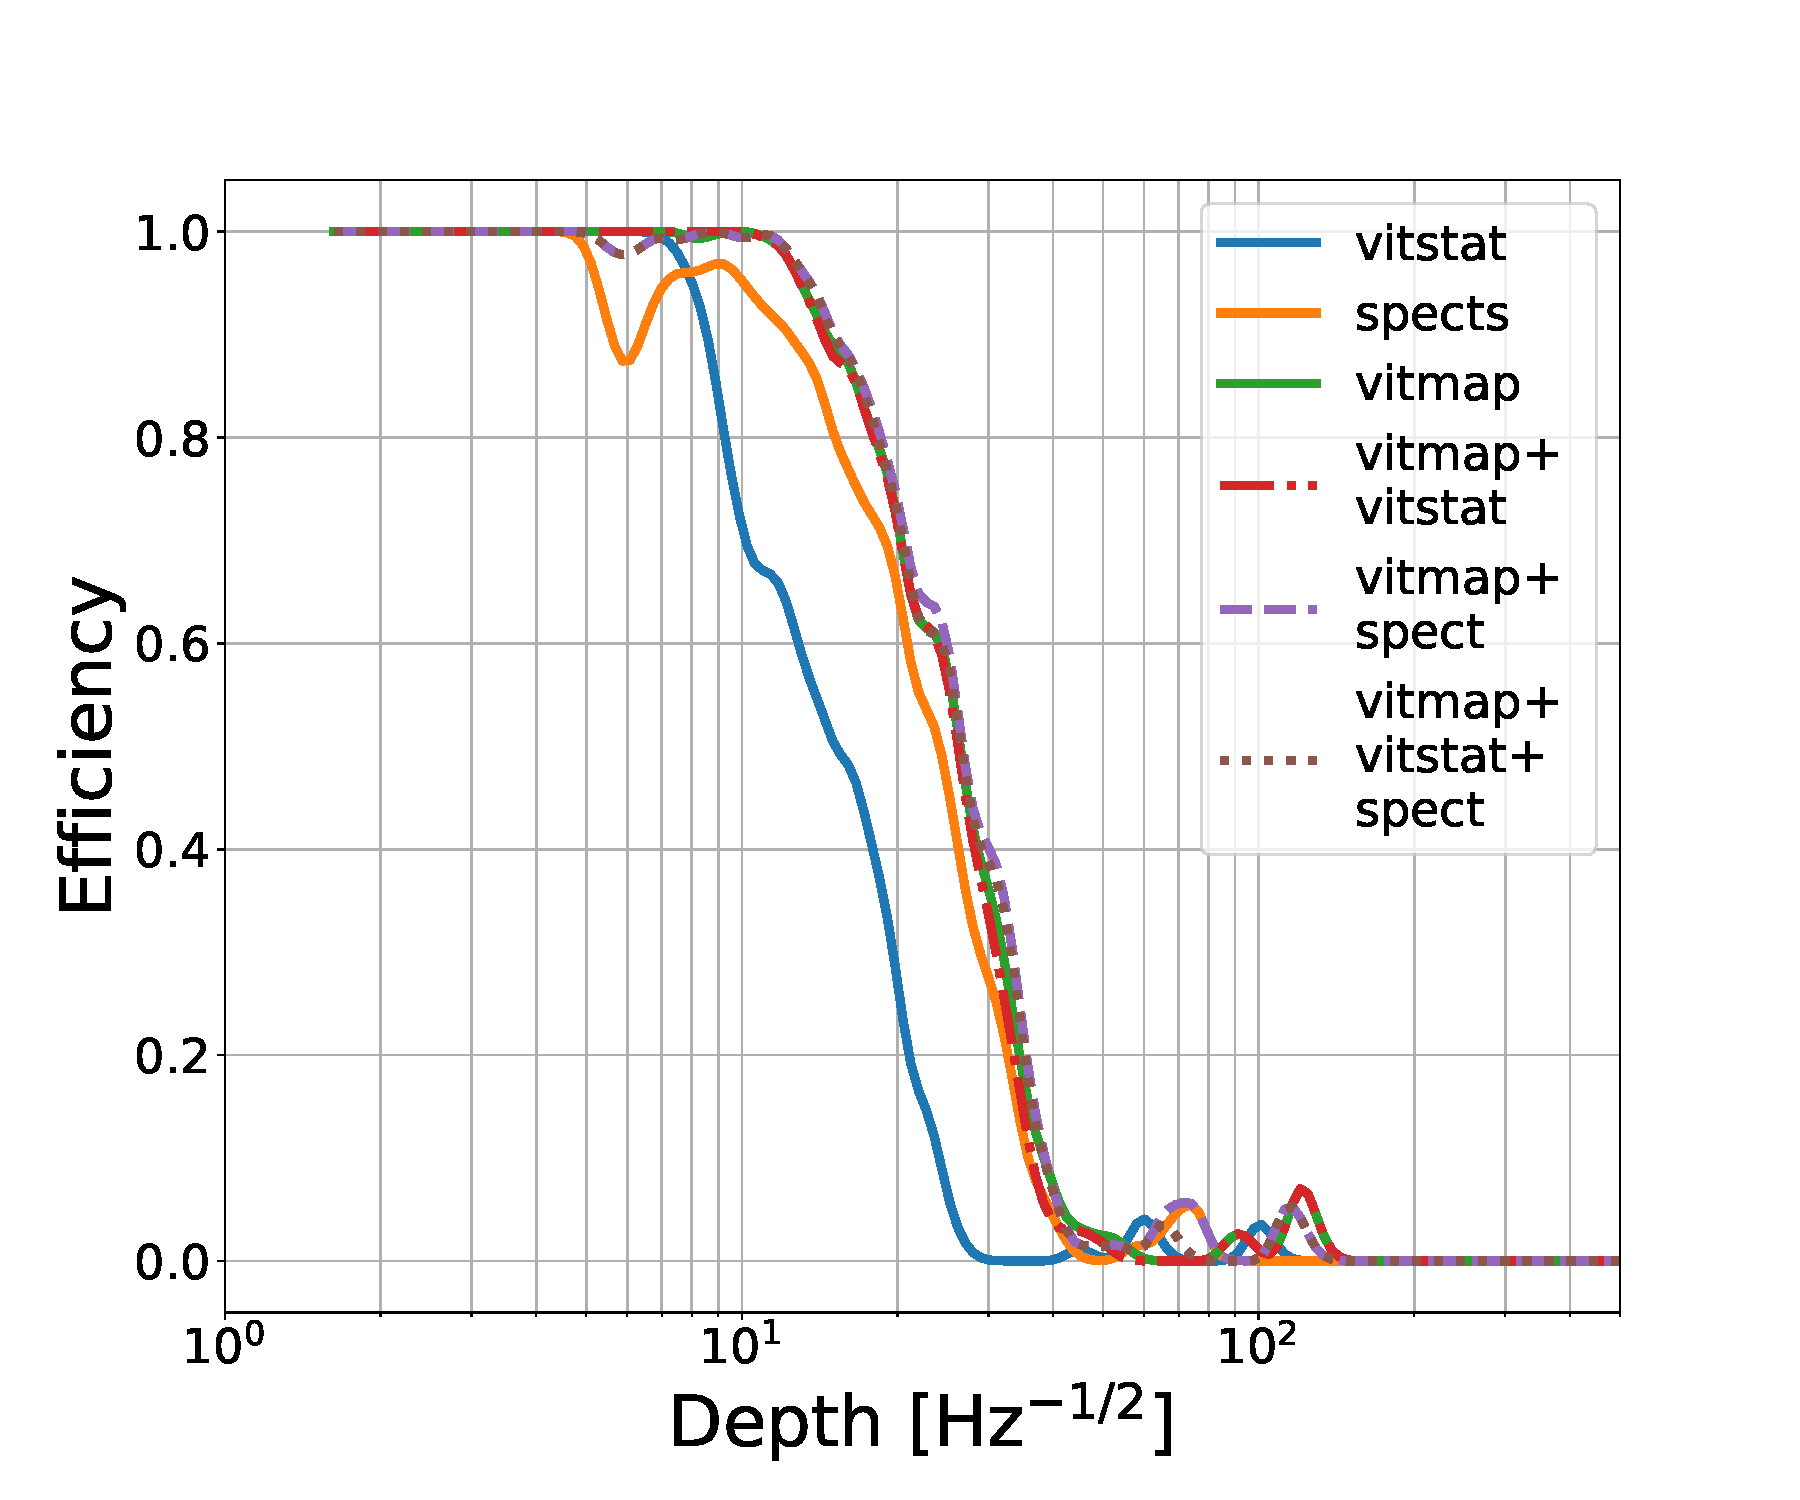
\includegraphics[width=\columnwidth]{C4_cnn/o2_depth_eff.pdf}
		\caption{}
		\label{machine:results:depth_o2}
	\end{subfigure}
	\caption{\label{machine:results:o2} In the O2 data-set, each of the six \glspl{CNN} were tested. The efficiency plots above are for a 1\% false alarm rate. These show that the use of spectrograms and the Viterbi maps with \glspl{CNN} greatly improve the sensitivity when compared to the Viterbi statistic. For each \gls{CNN} which uses a combination of inputs it achieves a similar sensitivity to the \gls{CNN} which uses just the Viterbi map. This implies that the Viterbi map contains the most information out of the tested \glspl{CNN}. }
	
\end{figure}



%%%%%%%%%
\subsubsection{Gaussian noise}
%%%%%%%%%%%

The next test involves using injections into Gaussian noise. For this test we tried to replicate the S6 data-set without including instrumental artefacts such as lines. We included the same gaps in data as S6 and the noise floor of S6 was replicated by scaling the \gls{SNR} of any injection in any given \gls{SFT}. 
Fig.~\ref{machine:results:s6gauss} shows the sensitivity curves for the Viterbi statistic and Viterbi map \gls{CNN} for both the Gaussian noise run with S6 gaps and for injections into the S6 data-set. 
In the Gaussian noise data-set the curves for both statistics, Viterbi map and the Viterbi statistic, show very similar results, this is to be expected as the main use of the \gls{CNN} was to reduce the effect of instrumental lines, for which there is none in this data set. 
The advantage of using the Viterbi maps in a \gls{CNN} becomes clear which it is tested on injections into real data with many instrumental lines. 
The remaining curves in Fig.~\ref{machine:results:s6gauss} show these tests, and it becomes clear that the Viterbi map \gls{CNN} reduces the effect of instrumental lines and therefore increases the searches sensitivity. 
These tests in S6 also show that the effect of instrumental lines was far greater in this run than in O2. 
This is shown in Fig.~\ref{machine:results:o2} where the separation between the Viterbi statistic curves and the Viterbi map curves is much smaller than the S6 curves in Fig.~\ref{machine:results:s6gauss}.
For injections into Gaussian noise following S6 gaps we show that with a false alarm of 1\% the Viterbi map \gls{CNN} achieves a sensitivity of SNR $~85$ and sensitivity depth of $~20\; {\rm Hz}^{-1/2}$ with 95\% efficiency. For injections into real S6 data the search achieves a sensitivity of SNR $~115$ and sensitivity depth of $~11\; {\rm Hz}^{-1/2}$ with 95\% efficiency and 1\% false alarm. We can also see from Fig.~\ref{machine:results:s6gauss} that the sensitivity in Gaussian noise with S6 gaps is better than in real S6 data, so there are still some elements of the search which reduces the sensitivity.

\begin{figure}
	\begin{subfigure}[h]{0.5\textwidth}
		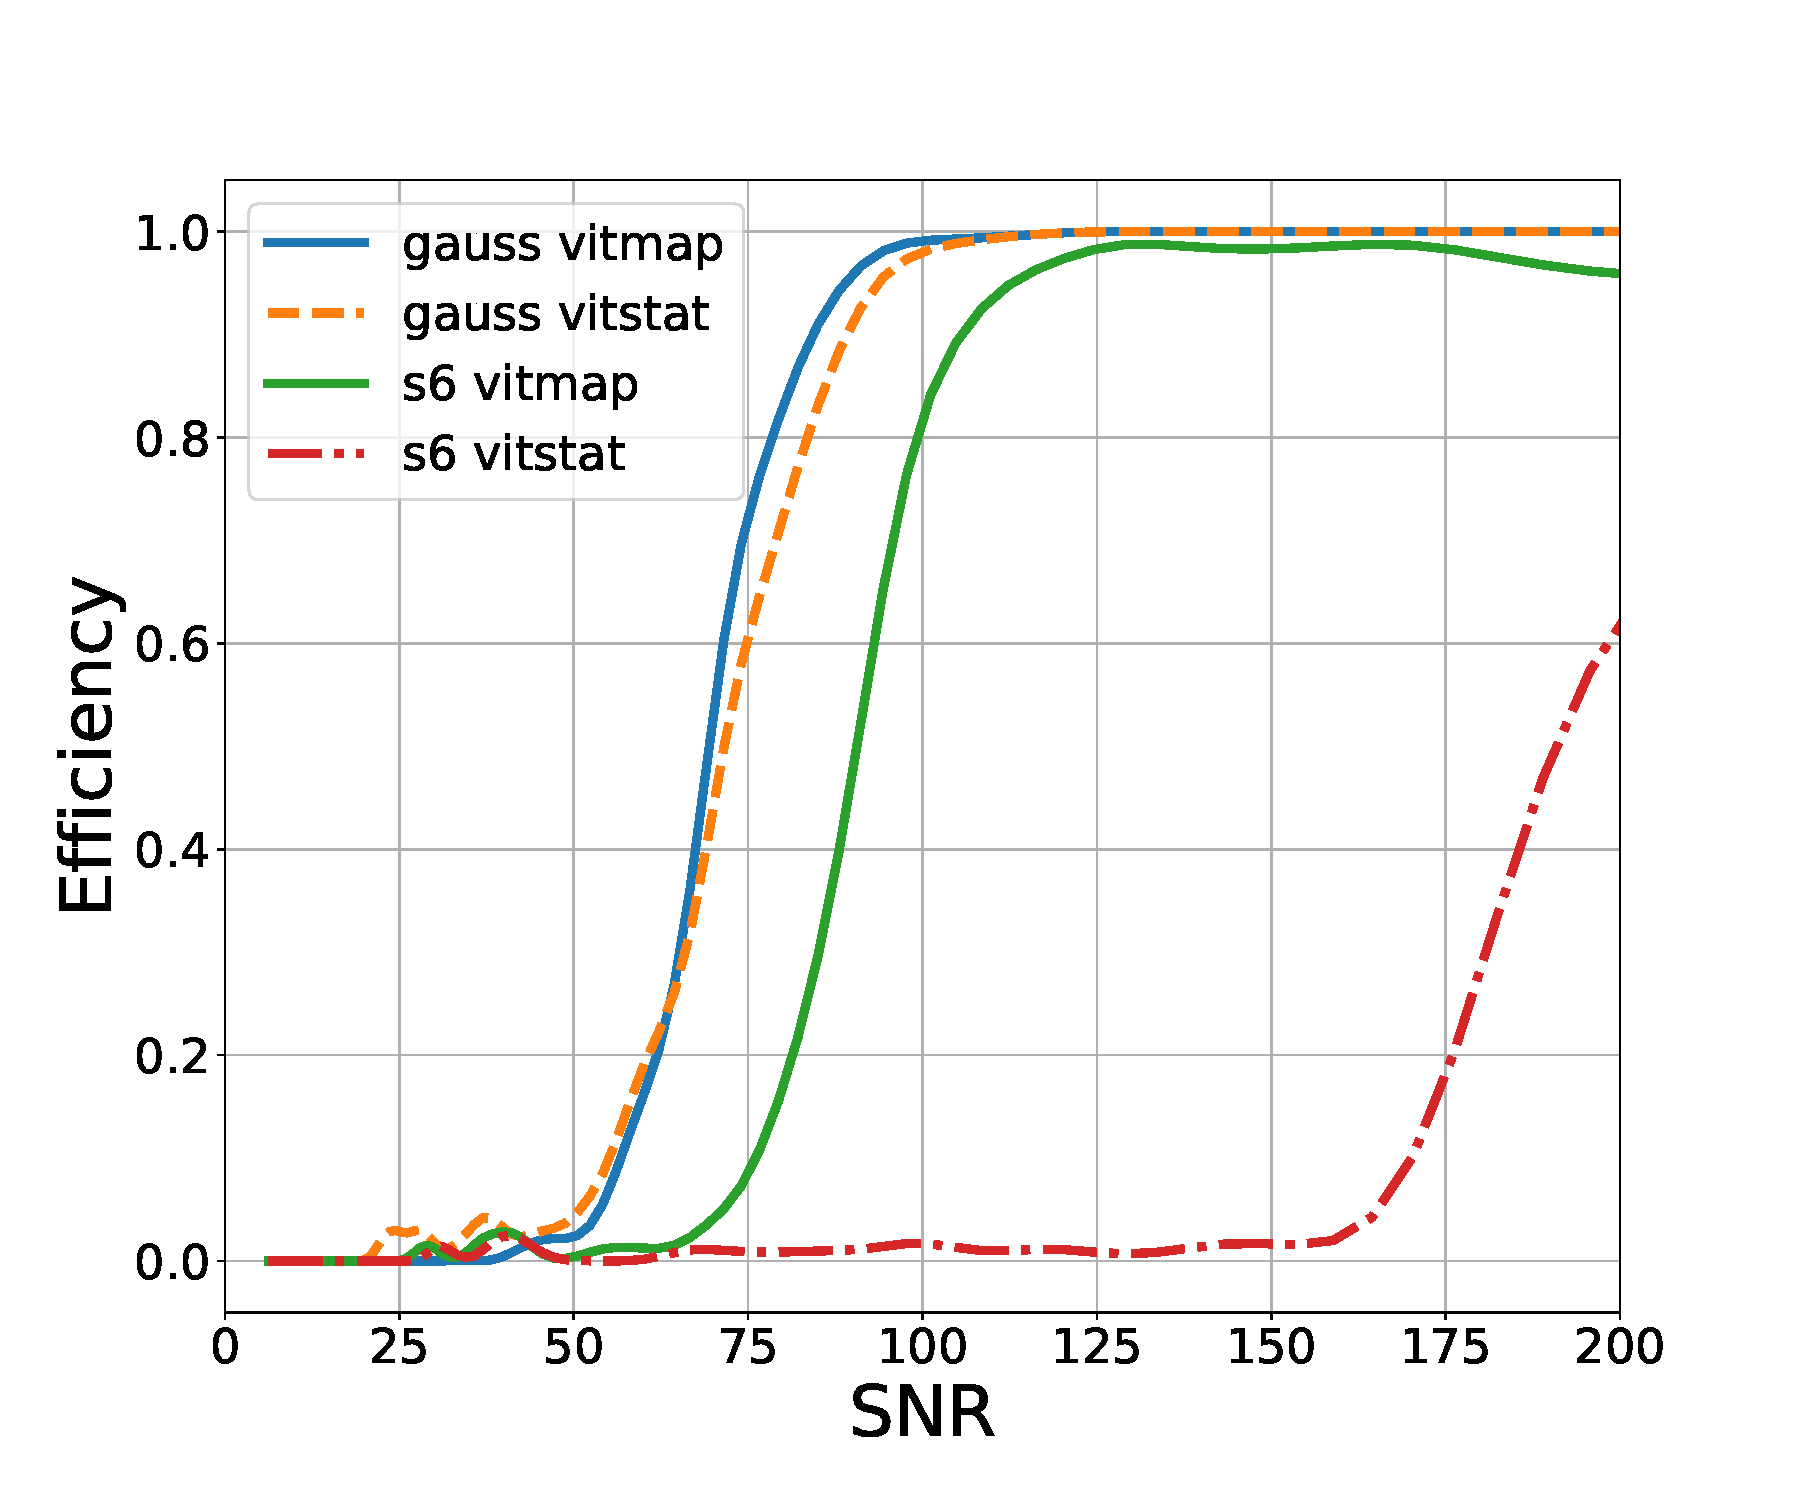
\includegraphics[width=\columnwidth]{C4_cnn/gauss_and_s6_snr_eff.pdf}
		\caption{}
		\label{machine:results:snr_s6}
	\end{subfigure}
	\begin{subfigure}[h]{0.5\textwidth}
		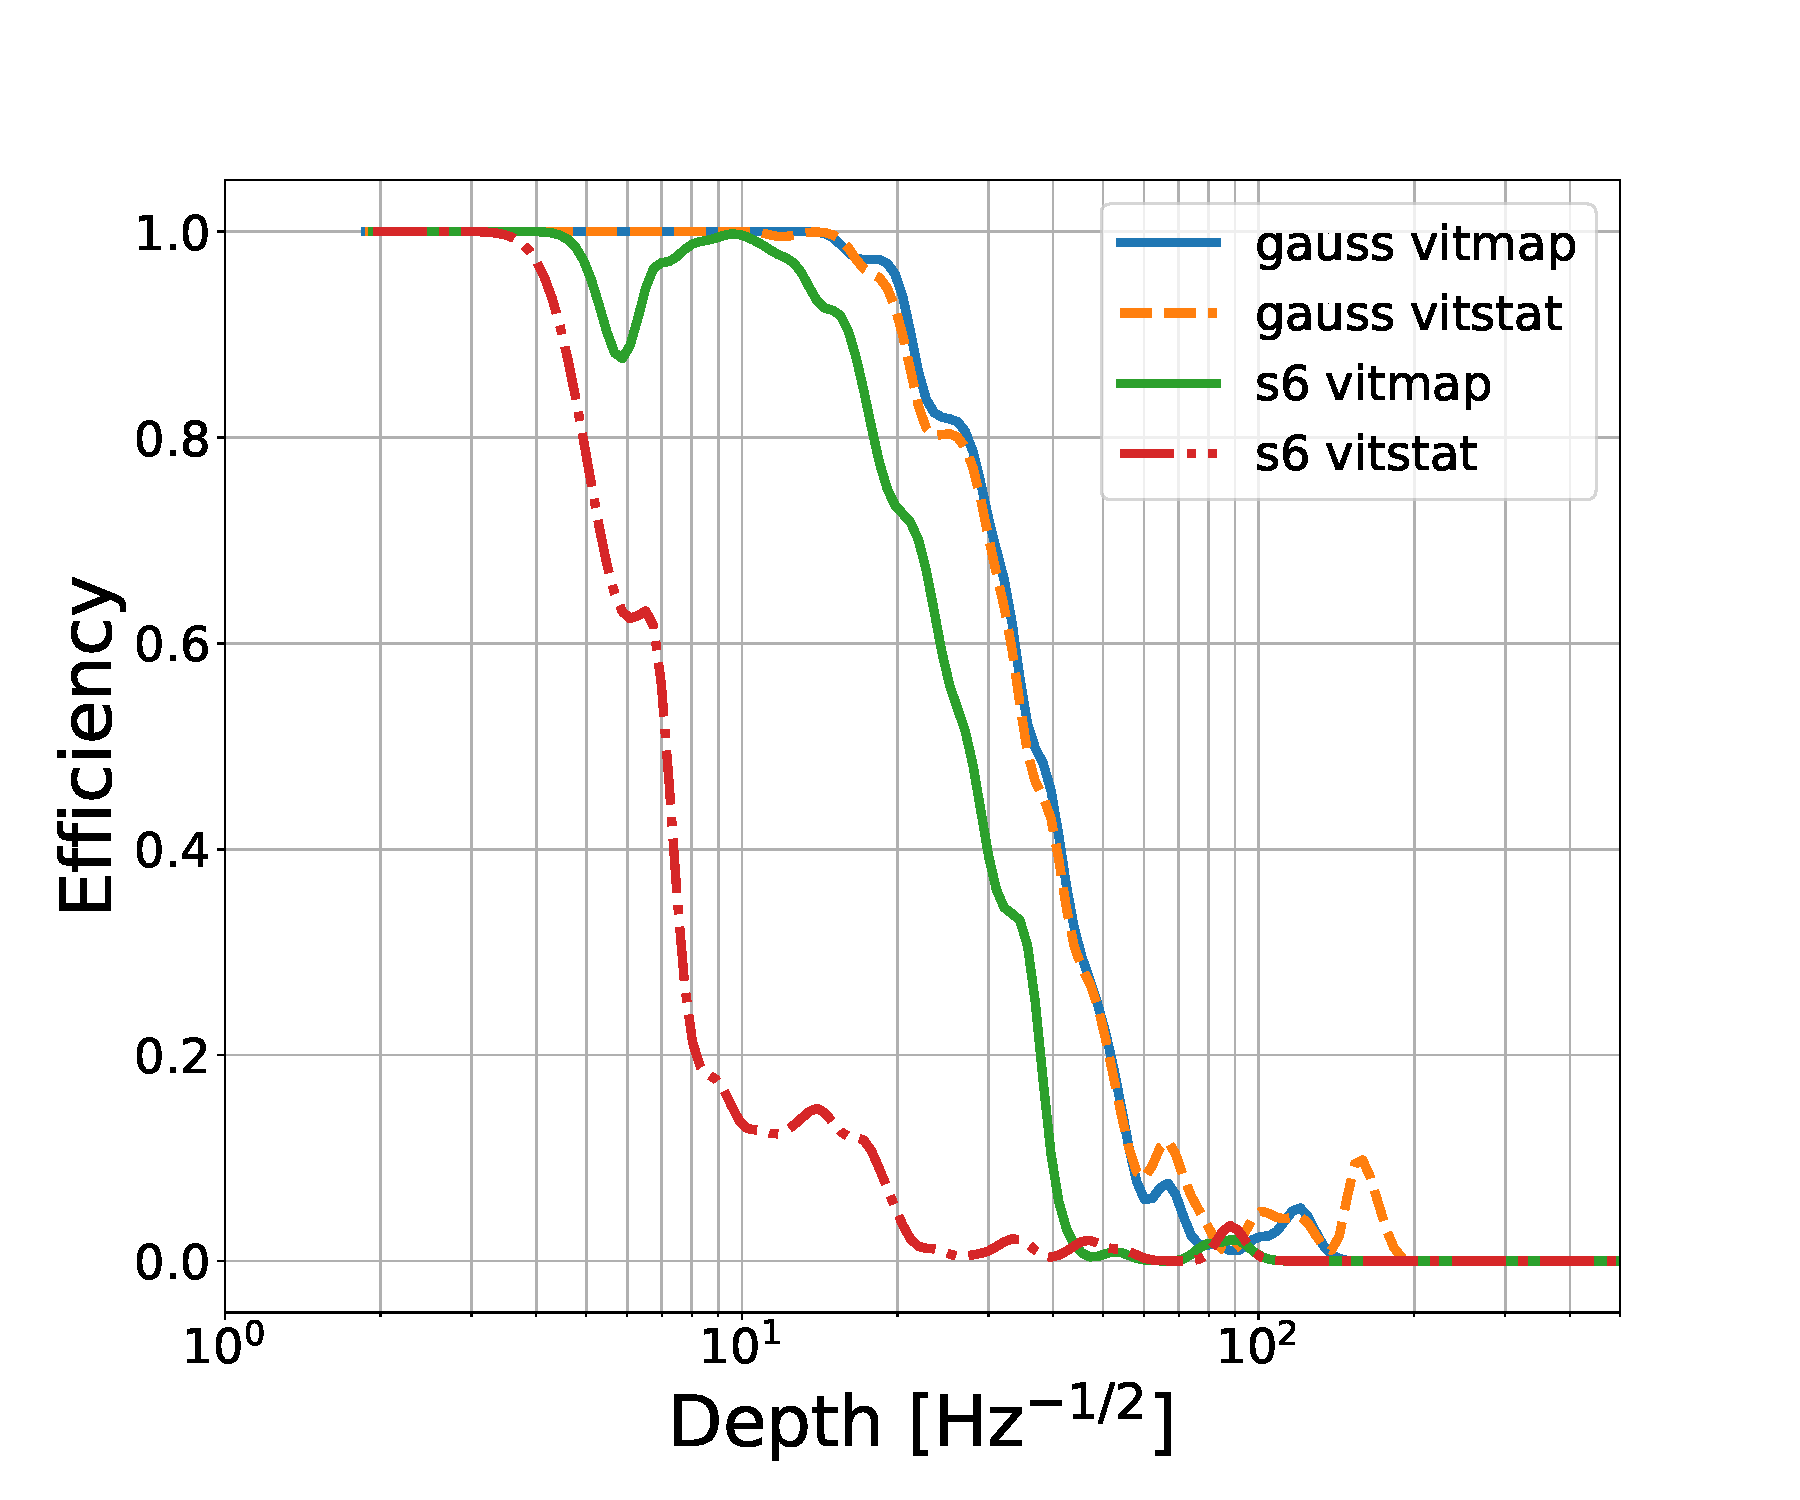
\includegraphics[width=\columnwidth]{C4_cnn/gauss_and_s6_depth_eff.pdf}
		\caption{}
		\label{machine:results:depth_s6}
	\end{subfigure}

	\caption{\label{machine:results:s6gauss} We aimed to compare the sensitivity of this search on simulations on real data (s6) to simulations in Gaussian noise (gauss). The Gaussian noise injections included the same gaps in data as the S6 data set. The \gls{SNR} of the simulated signal in Gaussian noise was adjusted based on the noise floor of S6. The sensitivity curves show that the Viterbi map \gls{CNN} (vitmap)achieves a similar sensitivity to the Viterbi statistic (vitstat) in Gaussian noise. This is because the main factor which effects the sensitivity of the Viterbi statistic is instrumental lines. As expected in real data, the Viterbi statistic is far less sensitive. The power of the \gls{CNN} becomes clear in tests on real data. The sensitivity of the Viterbi map \gls{CNN} is improved by over a factor of 2 in \gls{SNR} when tested on S6 data.}
	
\end{figure}

%%%%%%%
\subsubsection{S6}
%%%%%%%%%%

The final test was set up to again use the S6 data-set, however, we use a standard set of injections in the S6 \gls{MDC} \cite{walsh2016ComparisonMethods} to compare directly to other \gls{CW} search pipelines. In Fig.~\ref{machine:results:s6mdc} we show the results of the sensitivity curves from these injections. Fig.~\ref{machine:results:mdccomp} shows the direct comparison in depth of the results in \cite{walsh2016ComparisonMethods} with the results from the SOAP search with the Viterbi map \gls{CNN}. This shows that we achieve a sensitivity similar to many other semi-coherent searches with the exception of the Einstein@home search \cite{abbott2016ResultsDeepest}. For tests in the S6 \gls{MDC} we show that with a false alarm of 1\% the Viterbi map \gls{CNN} achieves a sensitivity of SNR $~90$ and sensitivity depth of $~16\; {\rm Hz}^{-1/2}$ with 95\% efficiency.


\begin{figure}
	\begin{subfigure}[h]{0.5\textwidth}
		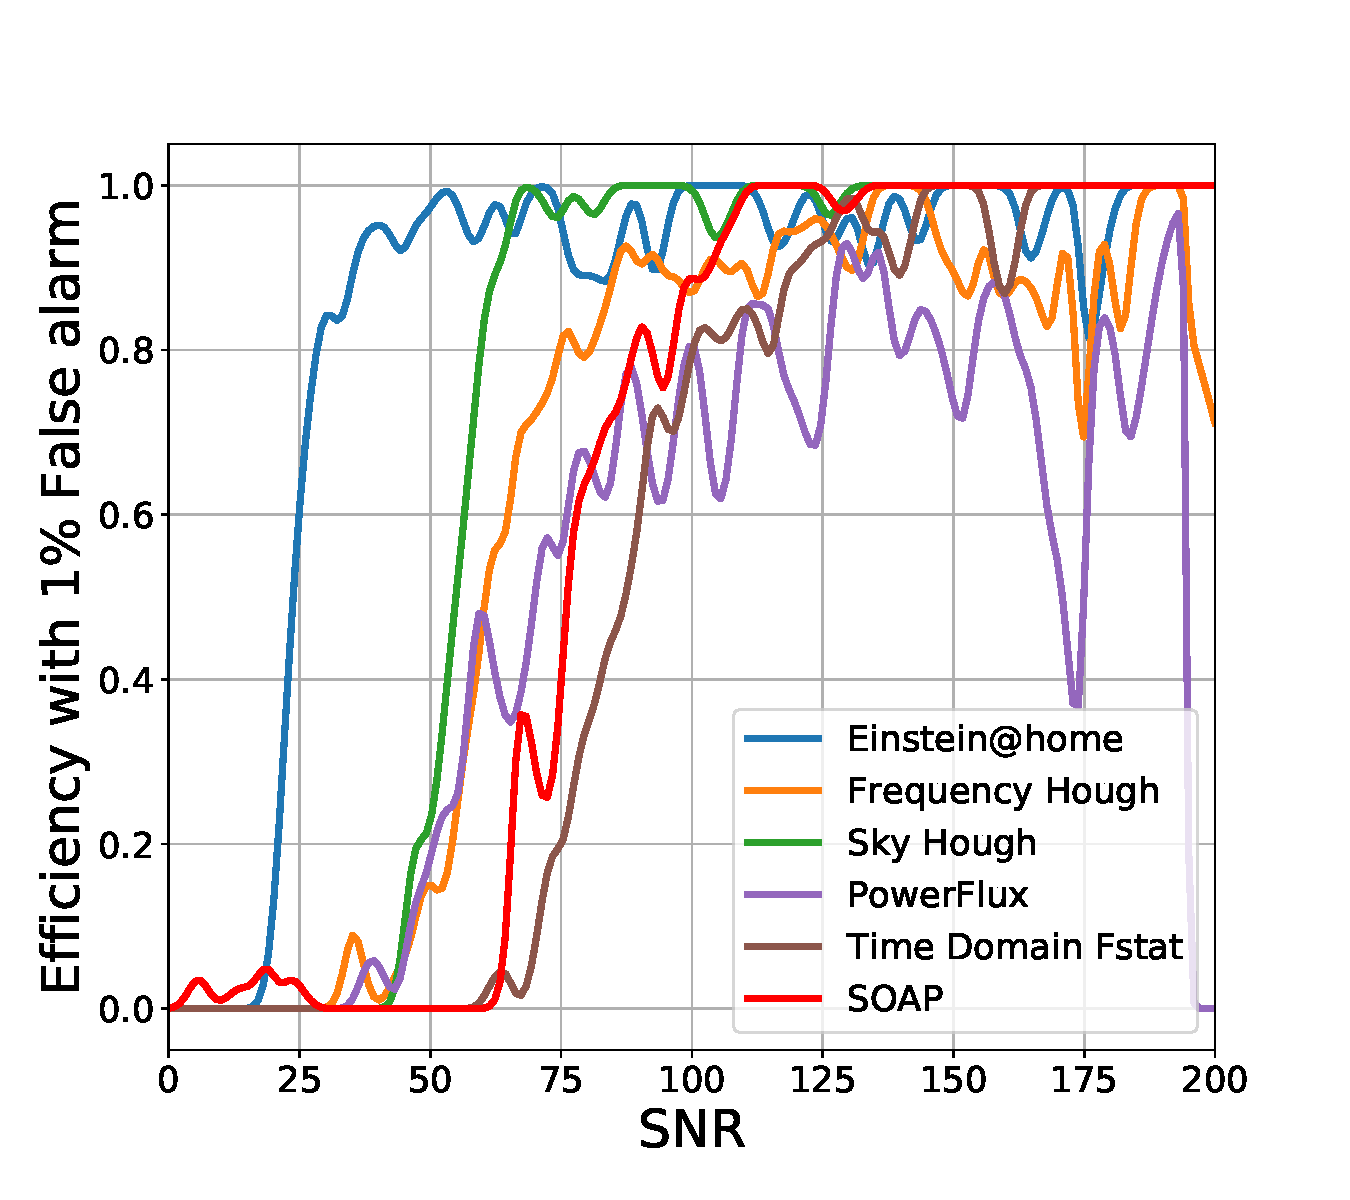
\includegraphics[width=\columnwidth]{C4_cnn/S6MDC_snr.pdf}
		\label{machine:results:snr_s6mdc}
	\end{subfigure}
\begin{subfigure}[h]{0.5\textwidth}
	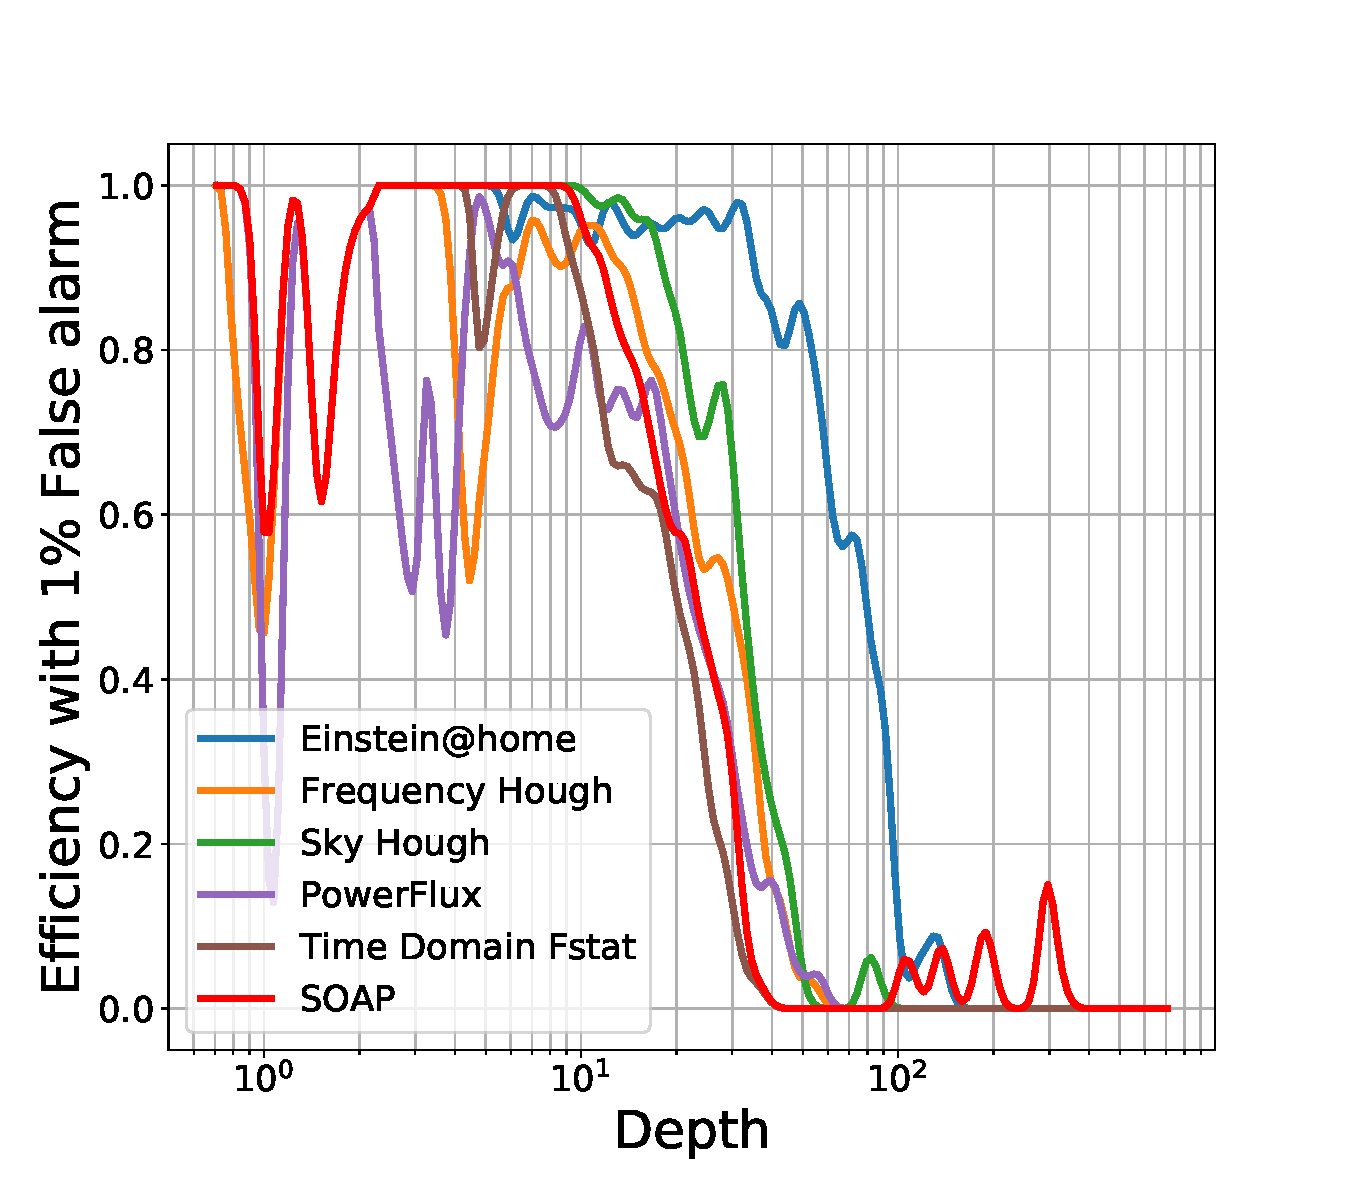
\includegraphics[width=\columnwidth]{C4_cnn/S6MDC_depth.pdf}
	\label{machine:results:mdccomp}
\end{subfigure}

	\caption{\label{machine:results:s6mdc} In the S6 \gls{MDC} \cite{walsh2016ComparisonMethods}, sensitivity curves were made for a set of \gls{CW} searches. 
		We have taken the list of detected pulsars for each search from this paper \cite{walsh2016ComparisonMethods} and replotted using the method in Sec.~\ref{machine:results:sensitivity} to compare the sensitivities. 
		This is results for all pulsar injections in the 40-500 Hz band in the S6 \gls{MDC}.
		This shows how the SOAP search with a \gls{CNN} achieves a similar sensitivity some other \gls{CW} searches. 
	}
	
\end{figure}


\subsection{\label{machine:results:timing} Computational time}

A key part of any \gls{CW} search is the computational time taken, the majority of the time for this search is used generating the appropriate data. 
For each section of the pipeline we have take the average total time for each job to complete, where each job runs on 2.0 Hz and it runs between 100 and 400 Hz. These are approximate timings taken for all the jobs to finish when run on CIT and can vary.

\begin{table}[h]
	%                     
	\centering                                                                                            
	\caption{\label{timing:table}Table shows the timings for each part of the search. These are approximate timings and vary when different amounts of data are input. This was run on data between 100-400 Hz.}
	
	%   
	\scalebox{0.8}{%
	\bgroup
	\def\arraystretch{1.5}
	\centering
	\begin{tabular}{c c c}
		\multicolumn{3}{c}{{\bf Generating data on CPU}}  \\
		\hline
		\hline
		& Time [hrs] & \\
		\hline
		Narrow-banding & $9$ &  \\
		\hline
		Training data& $239$ & \\
		\hline
		Test data& $75$ & \\
		\hline
		Search data& $40$ & \\
		\hline
		\hline
		\multicolumn{3}{c}{{\bf Training \glspl{CNN} on GPU} }  \\
		\hline
		\hline
		& Training time [hrs] & Loading time [hrs]\\
		\hline
		Viterbi statistic & $0.03$ & $0.2$ \\
		\hline
		Viterbi map & $0.8$ & $0.7$ \\
		\hline
		spectrogram & $9$ & $1$\\
		\hline
		Viterbi map \\ + Viterbi statistic& $1$ &$0.7$ \\
		\hline
		Viterbi map \\ + spectrogram& $1.4$ & $1.6$\\
		\hline
		Viterbi map \\ + Viterbi statistic \\ + spectrogram& $1.5$ & $2$ \\
		\hline
		\hline
		\multicolumn{3}{c}{{\bf Testing \glspl{CNN} on real data on GPU}}  \\
		\hline
		\hline
		& Testing [s] & Loading [s] \\
		\hline
		& $5$ & $60-160$ \\
		\hline
		\hline
	\end{tabular}
	\egroup
}
\end{table}

This gives the entire search including testing a total run time of $ \sim 386$ hours, however, the majority of the time is taken generating data which can be easily parallelised. 
Rather than taking hundreds of hours, the generating data sections takes $\mathcal{O}(1)$ hours in real time.


%%%%%
%%%%%
\section{\label{machine:results:sens_size} Sensitivity with the size of dataset}
%%%%%
%%%%%

When training a network, the general rule is that the more data the better. 
More data can limit effects such as over-training mentioned in Sec.~\ref{machine:training}.
To investigate how the sensitivity of the search changes with the number of training examples, the Viterbi map (vitmap) network in Sec.\ref{machine:results} was trained using a range of sizes of the training set. 
These networks are then tested on the same dataset to see how they perform.
This was repeated for two data-sets: \gls{CW} simulations in Gaussian noise and simulations in \glspl{LIGO} O1 data-set. 
For both of these cases six different networks were trained, these used: 100, 500, 1000, 5000, 10000 and 15000 Viterbi maps as their training datasets.
Each of these different sizes of training data is a randomly selected subset of the training data used in Sec.~\ref{machine:results:sensitivity}.
The test data for each was the same entire tests sets as in Sec.~\ref{machine:results:sensitivity}.

In the Gaussian noise case, the majority of the networks performed the same. 
Fig.~\ref{machine:results:sens_size:gauss_sens:eff} shows that in the Gaussian noise case, the majority of the networks performed with approximately the same sensitivity. 
This is with the exception of the network which was trained with 100 input Viterbi maps. 
Fig.~\ref{machine:results:sens_size:gauss_sens:train} shows that the sensitivity does appear to decrease, however, this is only by a few values in \gls{SNR}.
The implication of this is that the information in the Viterbi maps is relatively easy to extract when simulations are in Gaussian noise. 
In this case the network is trying to distinguish Gaussian noise from a simulated \gls{CW} signal.
Therefore, one would expect this to be an easier problem for the network to solve than when trying to distinguish an \gls{CW} signal from instrumental lines and Gaussian noise. 

\begin{figure}[h]
	\begin{subfigure}[h]{0.5\textwidth}
		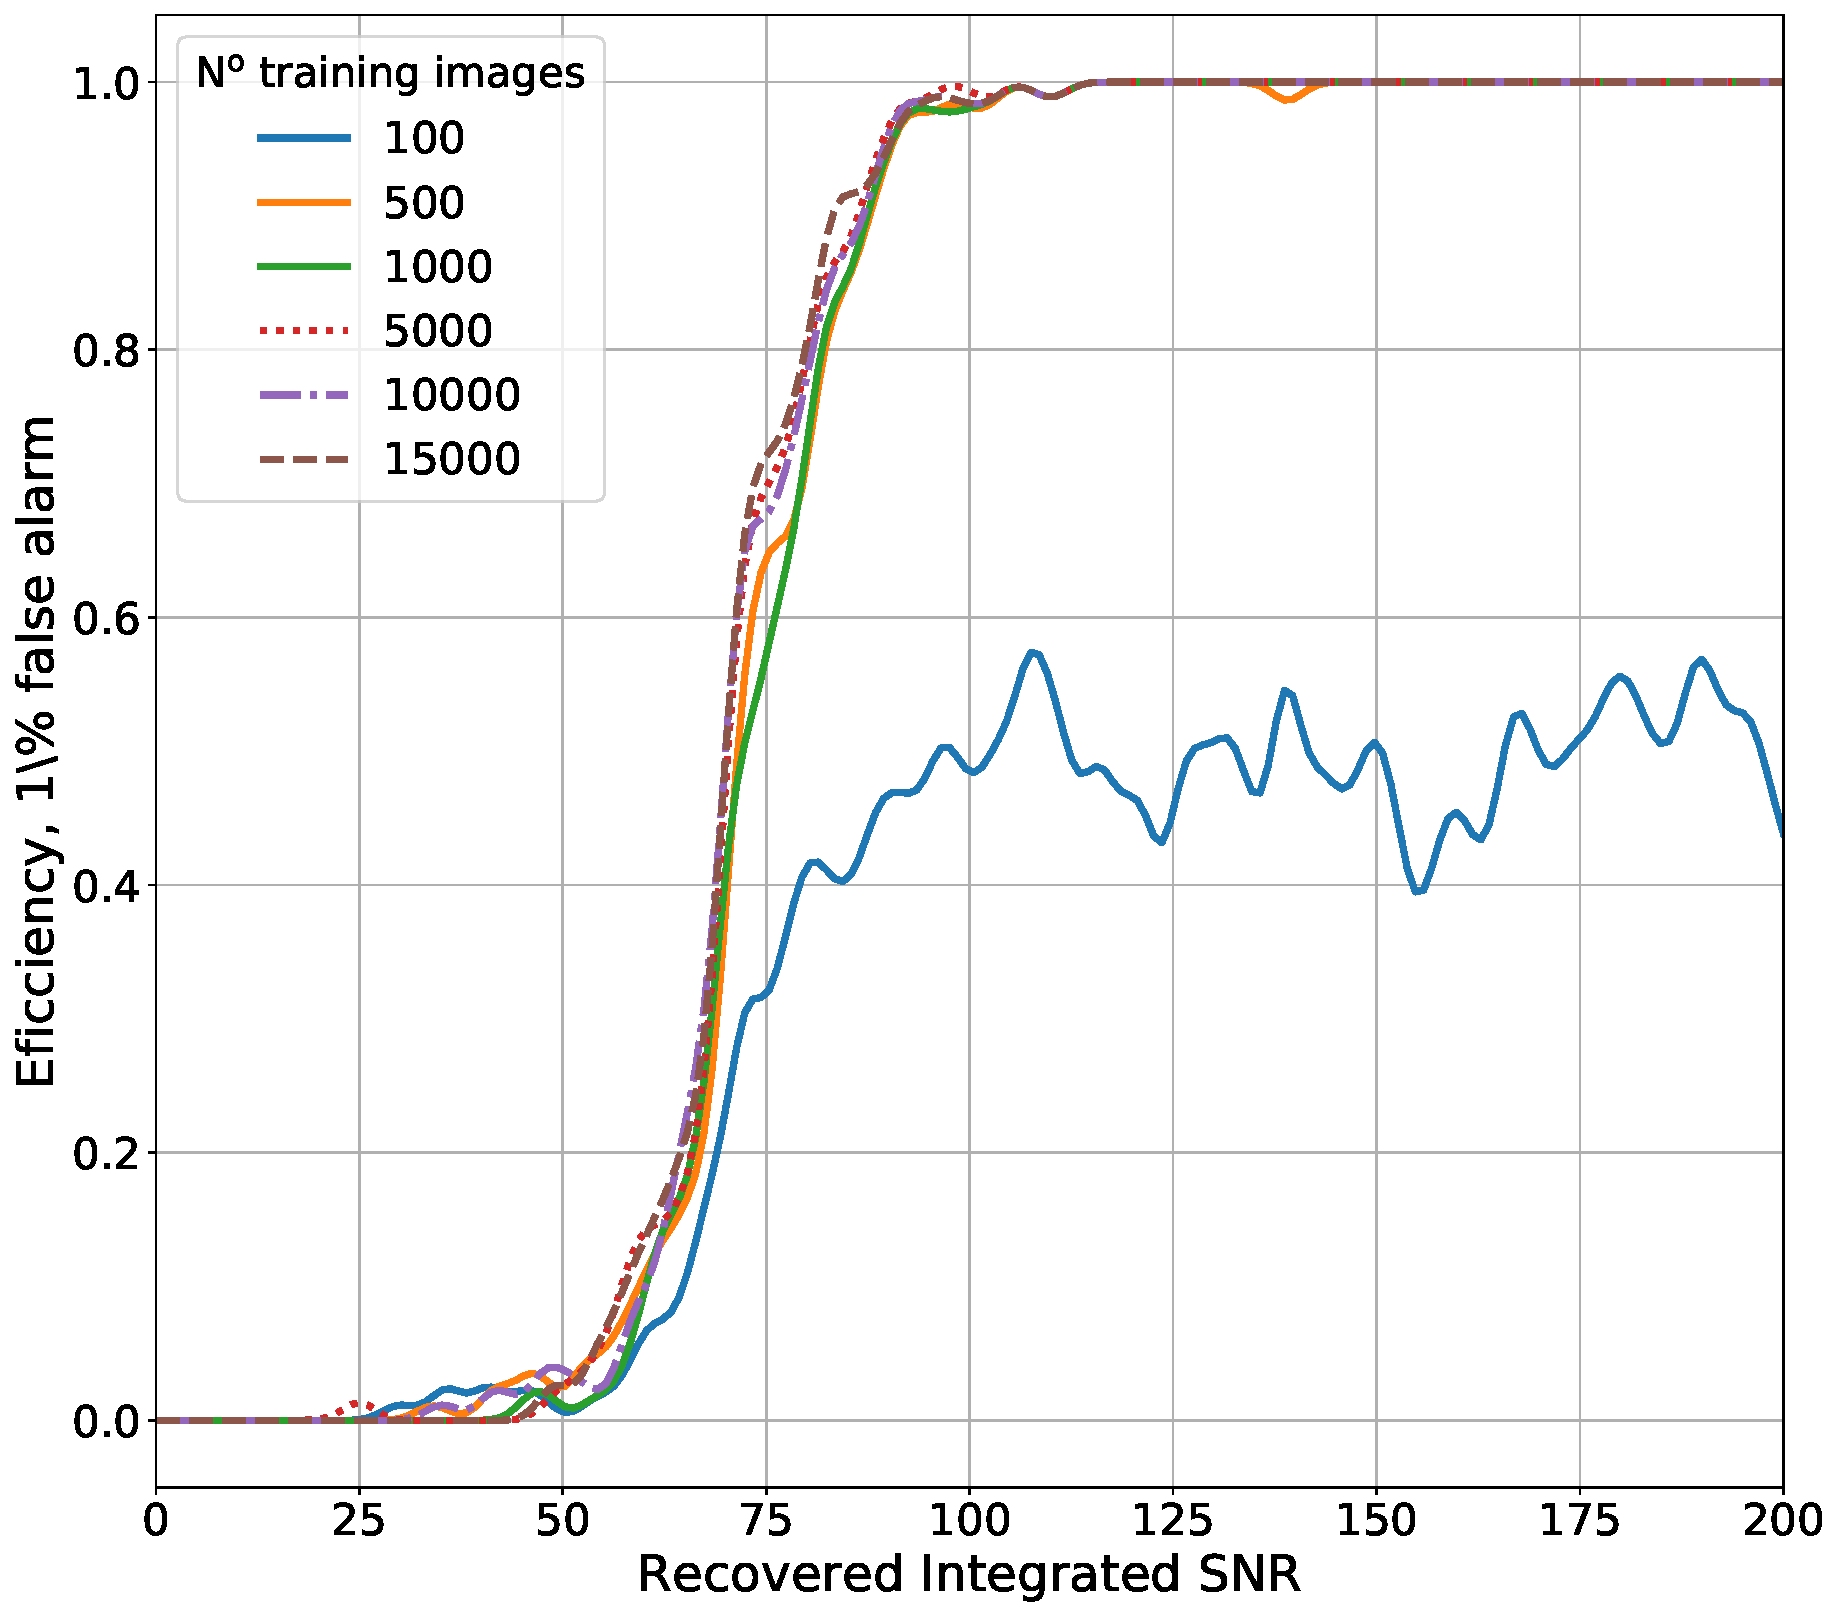
\includegraphics[width=\linewidth]{C4_cnn/gauss_sens_with_trainnum_eff.pdf}
		\caption{}
		\label{machine:results:sens_size:gauss_sens:eff}
	\end{subfigure}
	\begin{subfigure}[h]{0.5\textwidth}
		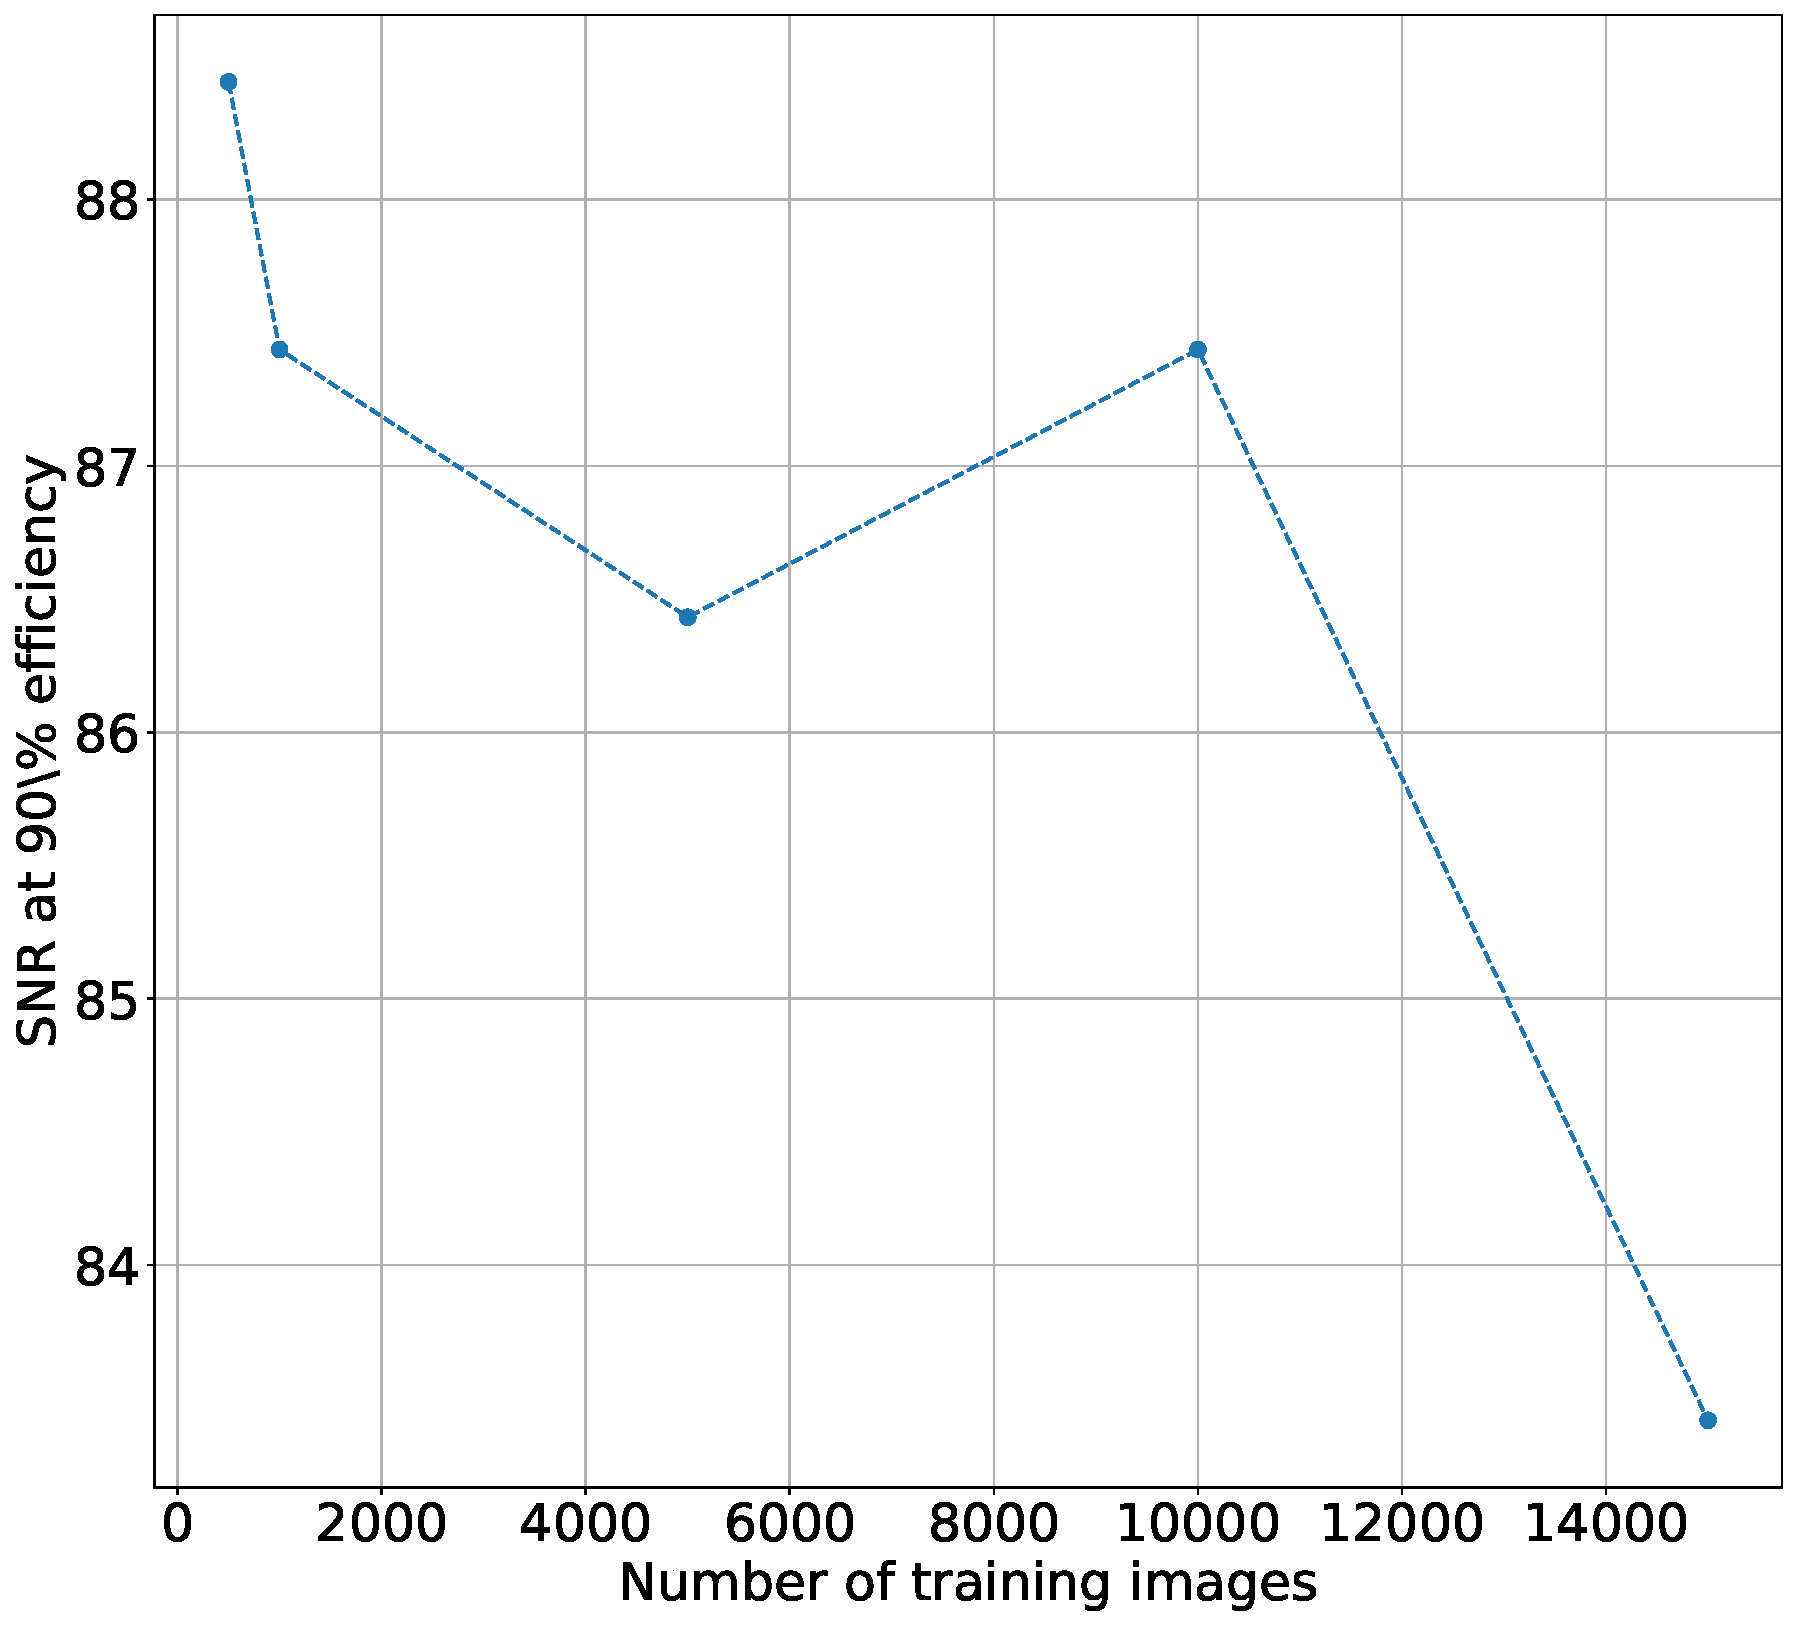
\includegraphics[width=\linewidth]{C4_cnn/gauss_sens_with_trainnum.pdf}
		\caption{}
		\label{machine:results:sens_size:gauss_sens:train}
	\end{subfigure}
	\caption{The amount of training data needed for an \gls{CNN} to perform well depends on the problem. Here I show how the sensitivity changes as a function of the number of training examples for simulations in Gaussian noise. Fig.~\ref{machine:results:sens_size:gauss_sens:eff} shows the efficiency curves for each of the different data-set sizes and Fig.~\ref{machine:results:sens_size:gauss_sens:train} shows the values of \gls{SNR} at 90\% efficiency as the data size increases. This shows that the increase in data size causes a slight increase in the sensitivity of the search. The efficiency curve for 100 training examples is not shows in Fig.~\ref{machine:results:sens_size:gauss_sens:train} as it does not reach the 90\% efficiency mark. \joe{would be nice to get some errorbars of some sort on the right hand side plot}}
	\label{machine:results:sens_size:gauss_sens}
\end{figure}

When simulating signals in real O1 data, many of the sub-bands will contain instrumental lines. 
The noise class for the networks then contains many variations compared to the Gaussian noise case. 
This a harder challenge to the neural network by essentially increasing the size of the parameter space.
Because of this, one would expect the network to need many more training examples to be able to achieve a similar sensitivity to Gaussian noise.
In Fig.~\ref{machine:results:sens_size:o1_sens:eff}, one can see that using 100 training examples is not enough and the network does not achieve any sensitivity at any \gls{SNR}. This means that the \gls{CNN} cannot classify any injection as detected using this number of training examples.
Fig.~\ref{machine:results:sens_size:o1_sens:train} seems to agree that real data poses a harder problem as the sensitivity drastically increases as the number of training examples is increased.
Therefore, more training examples are needed for the network to perform well on real data.

\begin{figure}[h]
	\begin{subfigure}[h]{0.5\textwidth}
		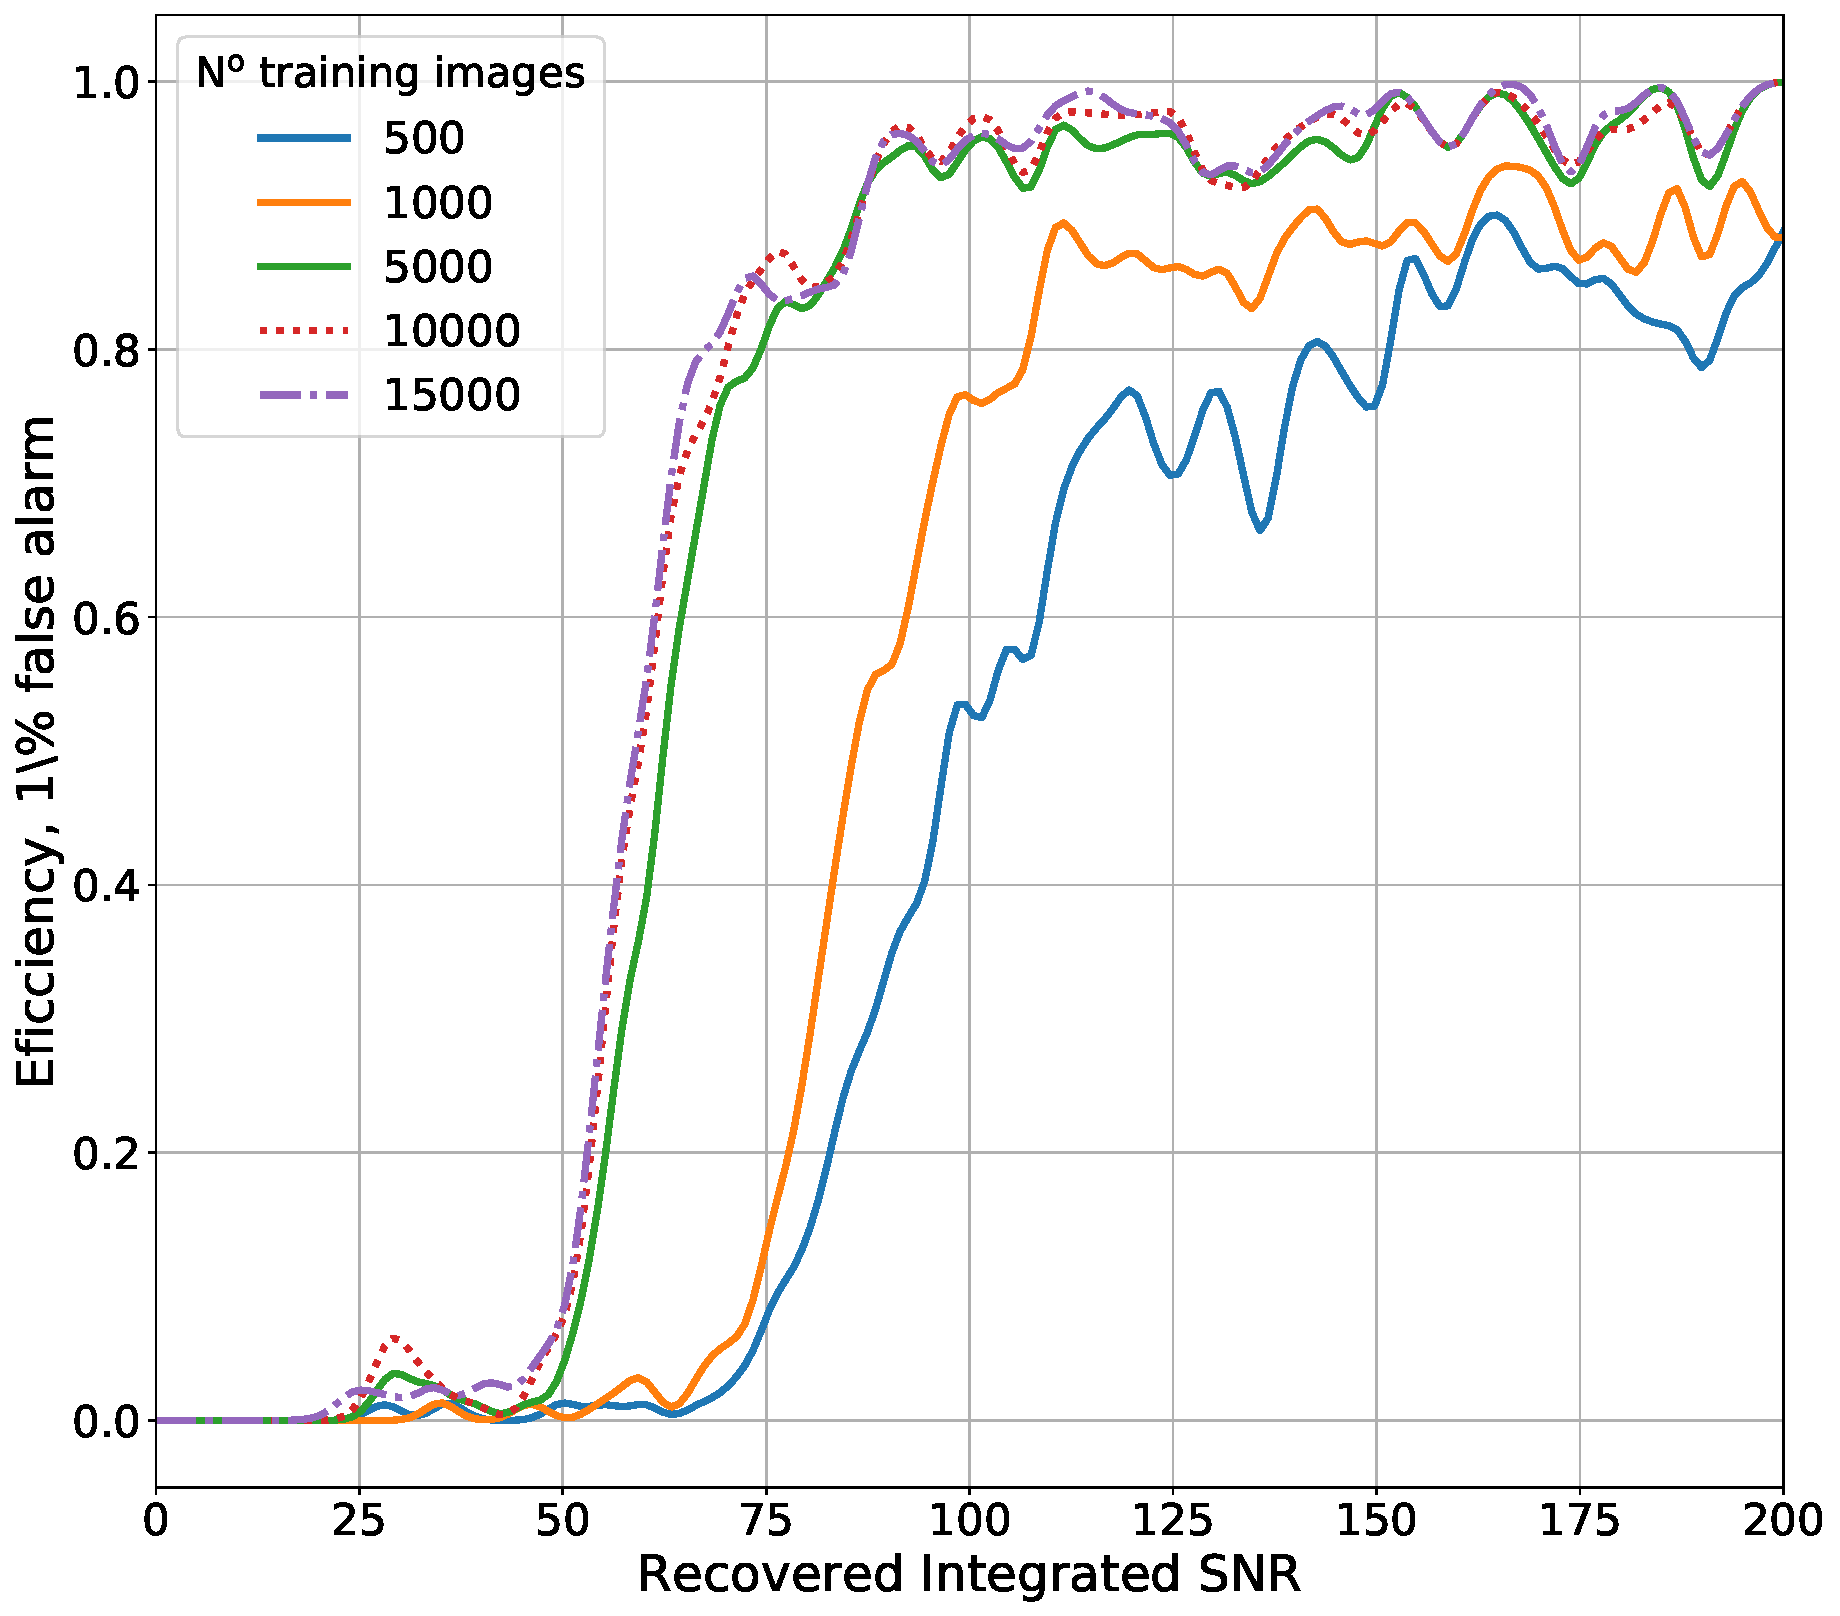
\includegraphics[width=\linewidth]{C4_cnn/o1_sens_with_trainnum_eff.pdf}
		\caption{}
		\label{machine:results:sens_size:o1_sens:eff}
	\end{subfigure}
	\begin{subfigure}[h]{0.5\textwidth}
		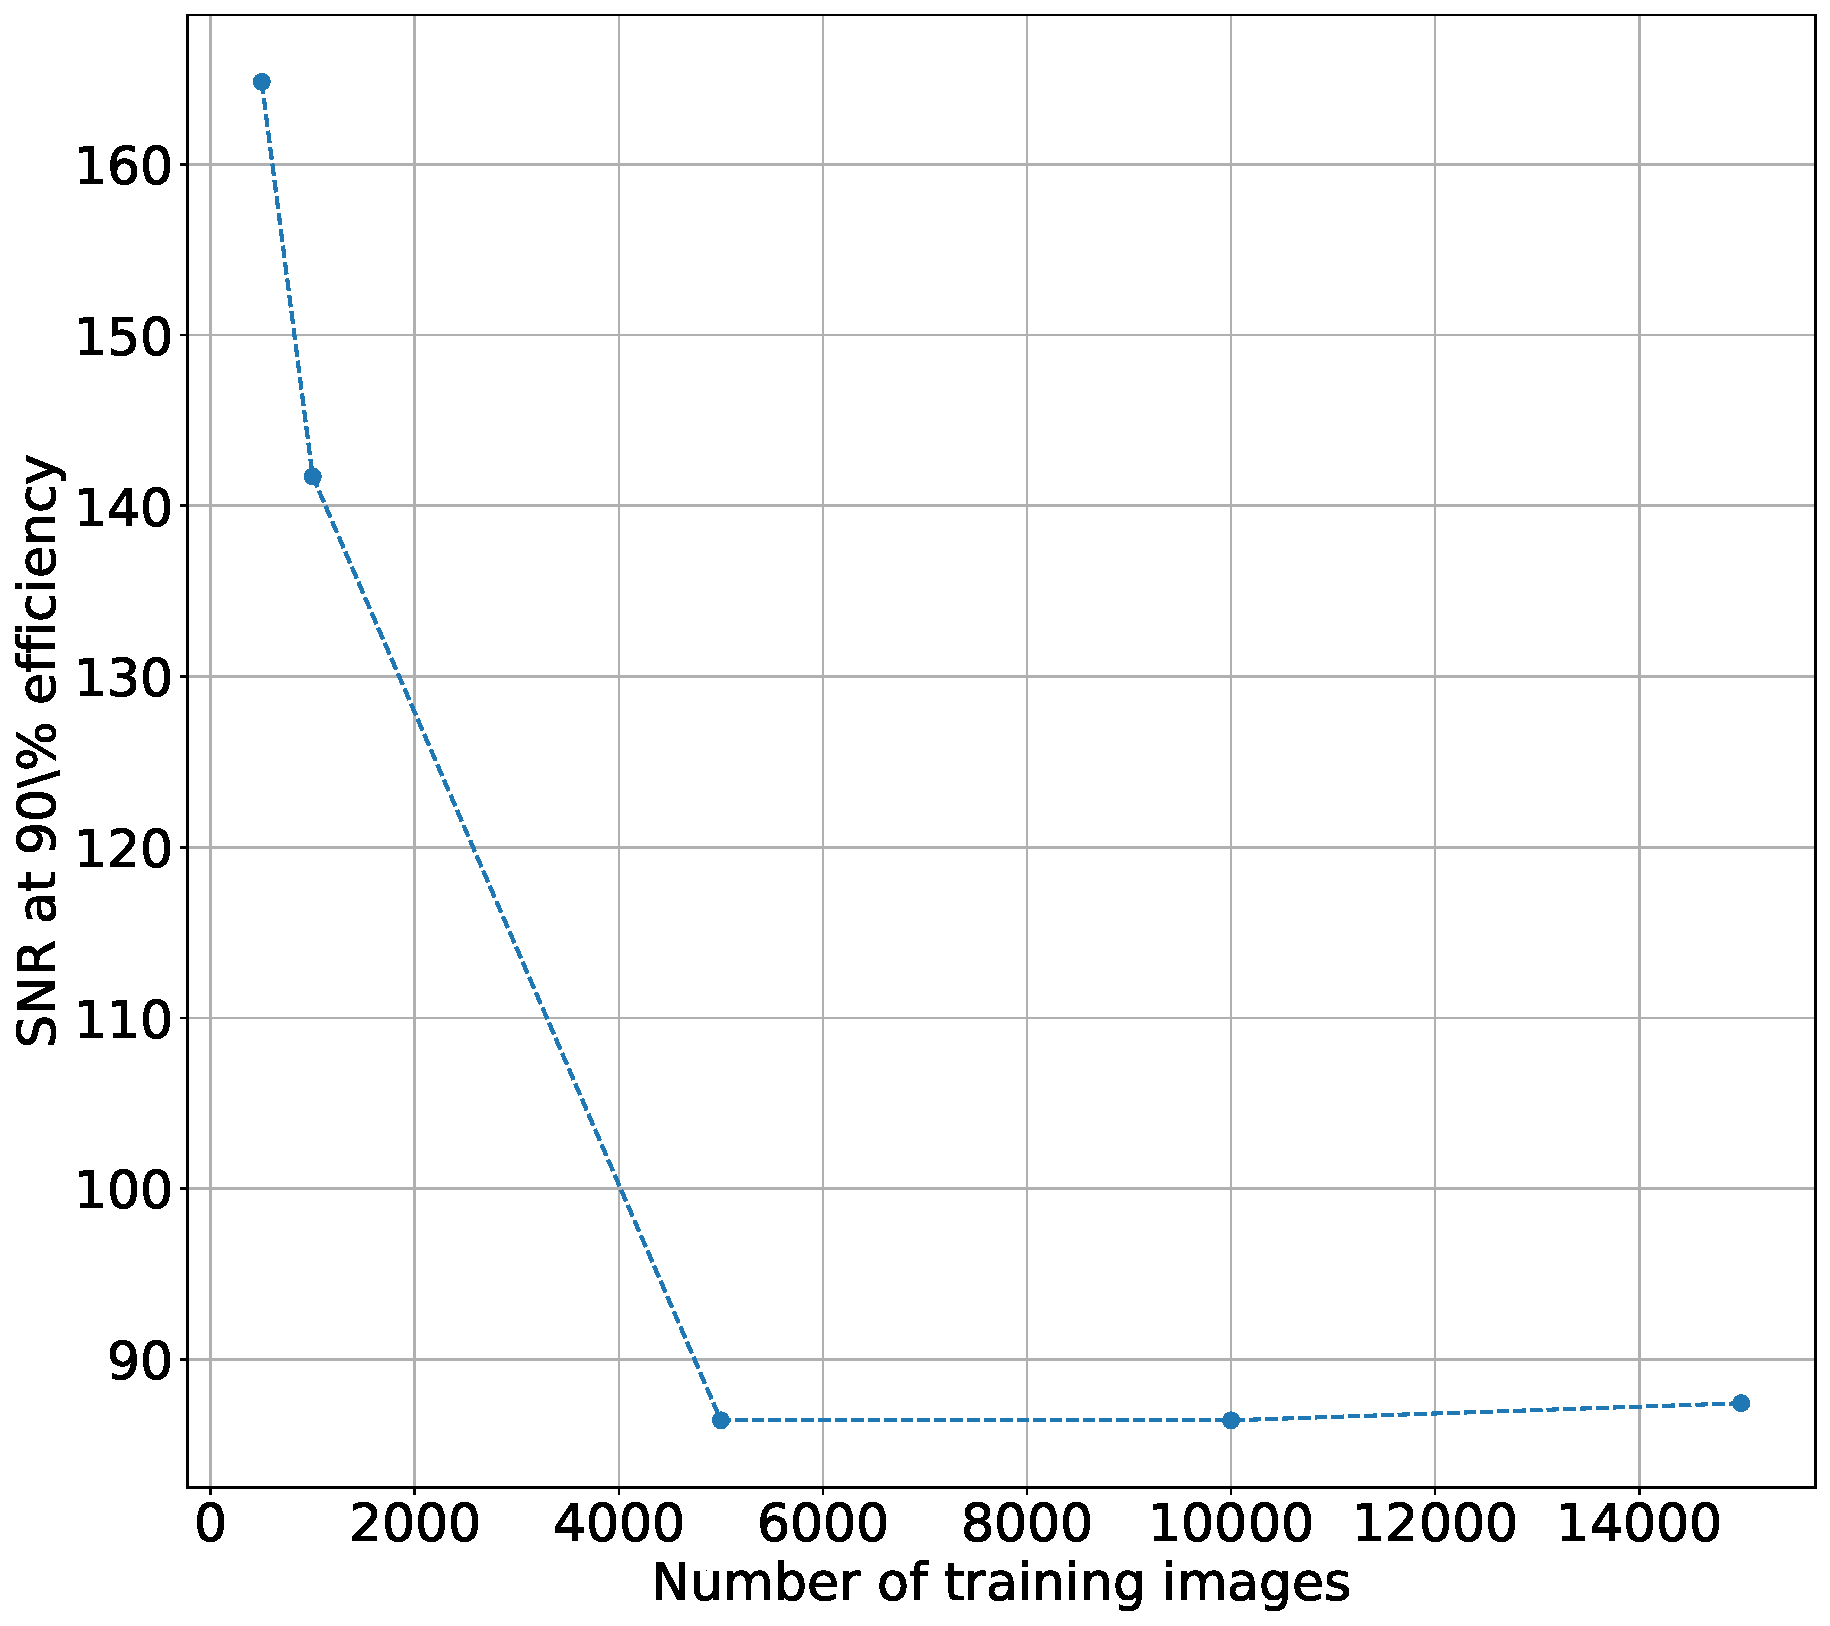
\includegraphics[width=\linewidth]{C4_cnn/o1_sens_with_trainnum.pdf}
		\caption{}
		\label{machine:results:sens_size:o1_sens:train}
	\end{subfigure}
	\caption{Here I show how the sensitivity changes as a function of the number of training examples for simulations in O1 data. Fig.~\ref{machine:results:sens_size:o1_sens:eff} shows the efficiency curves for each of the different data-set sizes and Fig.~\ref{machine:results:sens_size:o1_sens:train} shows the values of \gls{SNR} at 90\% efficiency as the data size increases. This shows that the increase in data size causes a large increase in the sensitivity of the \gls{CNN}. The efficiency curve for 100 training examples is not shows in Fig.~\ref{machine:results:sens_size:o1_sens:train} as it does not reach the 90\% efficiency mark.}
	\label{machine:results:sens_size:o1_sens}
\end{figure}



%%%%%%%%%%%
%%%%%%%%%%%
\section{\label{cnn:networkvis}Network Visualisation}
%%%%%%%%%%%
%%%%%%%%%%%

Neural network are generally hard to visualise due to the large number or parameters in the network that have to be varied.
However, there are methods which can be used to see how input data is affected by the network.
This can be useful to see how the network performs when given certain types of data and gives some insight into how the networks work

In the examples above we use \glspl{CNN}, the first few layers of this are build using convolutional filters.
The filters weights should ideally correspond to the shape of the feature which one wants to extract from the image. 
Generally this is only useful to picture at the first layer as the network can make subsequent layer and representations quite abstract.



\begin{figure}[h]
	\centering
	\includegraphics[width=\textwidth]{C4_cnn/vitmap_cnn_visualisation_signal.pdf}
	\caption{This shows a visualisation of the convolution neural network used for Viterbi maps above}
	\label{cnn:vis:vitmap:signal}
\end{figure}


%%%%%%%%%
%%%%%%%%
\section{Summary}
%%%%%%%%%
%%%%%%%%%

In this paper we summarise an extension of the SOAP algorithm which makes use of a \gls{CNN} to limit the effect of instrumental lines in a search for sources of continuous gravitational waves.
The SOAP search has a number of outputs for a given input spectrogram, where the main focus here is the Viterbi statistic and the Viterbi map. 
The Viterbi statistic has previously been used as a measure of whether there is a signal in a given frequency band, and the Viterbi maps are images which have the same shape as the input spectrogram, but gives a likelihood that there is a signal in a given location. 
The aim of the \gls{CNN} was to use the Viterbi maps and spectrograms as input images such that each frequency band can be classified to either having a signal or not. 
This would then remove then need to manually look through frequency bands and remove ones which are contaminated with non astrophysical features. 

We tested 6 separate \glspl{CNN} which all take in different input data or different combinations of data as input. 
The three input data types are: the Viterbi statistic, the Viterbi map and the spectrograms which are summed and divided by a running median.
The aim of using different input data types is that each would provide a different piece of information than the others, this had the hope that the combinations of these should then increase our sensitivity. 
The tests found that the \gls{CNN} which uses the Viterbi map alone as input was more sensitive than any other which used a single data type as input. 
Each of the \glspl{CNN} which used a combination of input data types had a similar sensitivity to the Viterbi map \gls{CNN}, therefore, it is assumed that the Viterbi map provides the most useful information when detecting a signal. 
Given that the main aim of this paper was to reduce the effect of instrumental lines on the SOAP search, in Gaussian noise data, the \gls{CNN} search should achieve a similar sensitivity to the Viterbi statistic alone. 
The tests in Gaussian noise with S6 gaps showed that at a 95 \% efficiency and a 1\% false alarm rate the Viterbi statistic and Viterbi map achieved a sensitivity of SNR 95 and 90 respectively. 
When the same test was run in real S6 data at a 95 \% efficiency and a 1\% false alarm rate the Viterbi statistic and Viterbi map achieved a sensitivity of SNR 300 and 120 respectively.
This demonstrates that the Viterbi map has a much larger effect when used on real data due to the presence of many instrumental lines within real data. 

These tests were once again repeated using a standard set of injections into S6 data such that a direct comparison can be made with other \gls{CW} search pipelines. 
At a 95 \% efficiency and a 1\% false alarm rate the Viterbi map \gls{CNN} achieved a sensitivity of \gls{SNR} $ \sim 90$ and sensitivity depth $\sim 14 \; \rm{Hz}^{-1/2}$ .
We have shown that the SOAP + \gls{CNN} approach can achieve a similar sensitivity to other semi-coherent \gls{CW} search algorithms but with a greatly reduced computational cost.

This search also offers a lot of flexibility in the signal type which can be searched, in the above examples the focus is on isolated neutron stars such that a comparison can be made to other \gls{CW} searches, however, this search is un-modelled. By changing the input parameters of the search, different signal types can be searched over, and in the future we aim to test its ability to identify more exotic sources of \gls{GW}. 
Further to this, we aim to make minor modifications to this pipeline such that some of the source parameters can be approximated. This should then return enough information to pass onto a more sensitive search for the signal. 




\chapter{\label{par_est}Parameter estimation using SOAP}
%%%%%%%%%%%%
%%%%%%%%%%%%
%%%%%%%%%%%%
%%%%%
%\epigraph{\textit{``Everyone Knows That When You Make An Assumption, You Make An A** Out Of 'U' And 'Umption.``}}{ --- \textit{Samuel Jackson (Mitch Henessey)}, The Long Kiss Goodnight}

Throughout Chapters \ref{soap} and \ref{machine} we have developed
techniques that could identify whether a potential \gls{CW}
signal is present within a small frequency band of width $0.1$ Hz, and then
return the frequency track that the signal is most likely to follow.  This
provides the frequency bands in which a signal could be present, which is useful
for all-sky searches as it can limit the parameter space and therefore
computational time for deeper searches such as those described in
Sec.~\ref{searchcw:search:targeted}.  However, this only limits the parameter
space in frequency to a smaller frequency band, where there is still a large
parameter space which needs to be searched.  If the Viterbi track returned by
SOAP in Chapter \ref{soap} follows the frequency evolution of a \gls{CW}
source, then this track contains information on the sky position and frequency
evolution of the \gls{CW}.  If one could extract this information then the size
of the parameter space could be reduced for more sensitive coherent searches, decreasing their computational cost.

In this Chapter we will outline a Bayesian method that uses the output Viterbi tracks of the SOAP search in Chapter~\ref{soap} to return a subset of astrophysical parameters of a
source.  Section~\ref{par_est:freq} will outline the model of the frequency
evolution of a \gls{CW} from a source with a slowly varying frequency,
Sec.~\ref{par_est:bayes} will outline the Bayesian model for this analysis and
Sec.~\ref{par_est:results} will show the results from testing on simulated
signals.

%%%%
%%%%
\section{\label{par_est:freq}\gls{CW} source frequency evolution}
%%%%
%%%%

The SOAP search, both single and multi detector, returns a frequency track known as the Viterbi track, if this
track follows the frequency of a \gls{CW} source, then the frequency evolution
contains information of the sky position ($\alpha, \delta$), the frequency of
the source $f$ and its derivative $\dot{f}$, where we ignore higher order
frequency derivatives.  From the Viterbi track, we should then be able to
extract this information as we have a model for the phase evolution (and
therefore frequency evolution) of the source described in
Eq.~\ref{searchcw:model:phase} in Sec.~\ref{searchcw:model}.  To relate this
phase evolution to the sky position parameters, we can look closer at
Eq.~\ref{searchcw:model:ssbtime}, where we describe the shift in arrival time
due to the Earth's motion.

The second term in Eq.~\ref{searchcw:model:ssbtime} describes the Doppler shift
due to the earth's orbit and rotation.  Where the $\bm{r}$ is the position of
the detector and $\bm{n}$ is a unit vector in the direction of the source.  As
in \citep{schutz1998DataAnalysis}, we use the ecliptic coordinate frame in the \gls{SSB}
where the $z$ axis is perpendicular to the ecliptic and the $x$ axis points towards the first point of Aries.  In this frame the unit vector pointing
towards the source can be written as
%
\begin{equation}
    \label{par_est:freq:unit}
    \bm{n} = 
    \left(
    \begin{matrix}
        1 & 0 & 0  \\
        0 & \cos \epsilon & \sin \epsilon \\
        0 & -\sin \epsilon & \cos \epsilon \\
    \end{matrix} \right)
    \left(
    \begin{matrix}
        \cos(\alpha)\cos(\delta)  \\
        \sin(\alpha)\cos(\delta) \\
        \sin(\delta) \\
    \end{matrix} \right),
\end{equation}
%
where $\alpha$ and $\delta$ are the right ascension and declination (sky
position) of the source and $\epsilon$ is the obliquity of the ecliptic, which is the inclination angle of the earths equator with respect to the ecliptic.  The first matrix in Eq.~\ref{par_est:freq:unit} describes
a rotation from the celestial frame to
the ecliptic frame an the second vector transforms the sky position parameters to their component $x,y,z$ coordinates in the celestial frame.

The position vector of the detector,
$\bm{r}$ in Eq.~\ref{searchcw:model:ssbtime}, at a time $t$ can be split into two components,
the position due to the orbit of the earth and position of the detector due to the rotation of
the Earth.
If we assume the orbit is circular, then the position of the earth in its orbit
is described in Cartesian coordinates as
%
\begin{equation}
    \bm{r}_{\rm{orb}} = R_{\mathrm{orb}}
    \left(
    \begin{matrix}
        \cos{\left( \Omega_{\mathrm{orb}} t   \right)}  \\
        \sin{\left( \Omega_{\mathrm{orb}} t   \right)} \\
        0 \\
    \end{matrix} \right),
\end{equation}
%
where $R_{\mathrm{orb}}$ is the radius of the earth's orbit (1 AU),
$\Omega_{\mathrm{orb}}$ is the angular frequency of the earth's orbit
$2\pi/T_{\mathrm{orb}}$, where $T_{\mathrm{orb}}$ is one year and the time $t=0$ is when the earth is at the spring equinox.  The
position due to the rotation of the earth can then be described by 
%
\begin{equation}
    \bm{r}_{\rm{rot}} = R_{\mathrm{rot}}
    \left(
    \begin{matrix}
        1 & 0 & 0  \\
        0 & \cos \epsilon & \sin \epsilon \\
        0 & -\sin \epsilon & \cos \epsilon \\
    \end{matrix} \right)
    \left(
    \begin{matrix}
        \cos{(\beta)}\cos{\left( \Omega_{\mathrm{rot}} t + \phi_{\mathrm{rot}}  \right)}  \\
        \cos{(\beta)}\sin{\left( \Omega_{\mathrm{rot}} t + \phi_{\mathrm{rot}}  \right)} \\
        \sin{(\beta)} \\
    \end{matrix} \right),
\end{equation}
%
where $R_{\mathrm{rot}}$ is the radius of the earth, $\Omega_{\mathrm{rot}}$ is the
angular frequency of the earth's rotation $2\pi/T_{\mathrm{R}}$, where
$T_{\mathrm{rot}}$ is one day and $\beta$ is the detectors latitude. The phase $\phi_{\mathrm{rot}}$ defines the position of the earth in its rotation at $t=0$ and is determined by $\phi_{\mathrm{rot}} = \rm{LST}_{t=0} = \rm{GMST}_{t=0} - \lambda$, where $\lambda$  is the longitude of
the detectors site, the \gls{GMST} is the angle between the first point of Aries and the Greenwich meridian and the LST is the local sidereal time. The sum of these two components
then define the location of the detector in the \gls{SSB} frame
%
\begin{equation}
    \bm{r} = \bm{r}_{\rm{orb}} + \bm{r}_{\rm{rot}}.
\end{equation}

We can now describe the phase evolution of the signal at the detector
sites (latitude $\beta$ and longitude $\lambda$) starting at a time $t=0$ from the source sky
position ($\alpha, \delta$), frequency $f$ and its derivative
$\dot{f}$.  We can write the phase evolution from Eq.~\ref{searchcw:model:phase} as
%
\begin{equation}
    \label{par_est:freq:ph_evolution}
    \begin{split}
        \Phi(t) = 2\pi \left(  f_0 t + \frac{\dot{f} t^2}{2} \right) &+ \frac{2\pi}{c} \left(  f_0 + \dot{f}t  \right) \left\{ R_{\rm{orb}} \left[ \cos \alpha \cos \delta \cos \left( \Omega_{\mathrm{orb}} t \right) \right. \right. \\ 
        &+ \left. \left( \cos \epsilon \cos \alpha \cos \delta +  \sin \epsilon \sin \delta \right) \sin \left( \Omega_{\mathrm{orb}} t  \right) \right] \\
        &+ \left. R_{\rm{rot}} \left[ \sin \beta \sin \delta + \cos \beta \cos \delta \cos \left( \alpha - \Omega_{\mathrm{rot}} t - \phi_{rot}  \right)     \right] \right\},
    \end{split}
\end{equation}
%
where we ignore frequency derivatives higher than first order.
The frequency of a \gls{CW} signal at any point on the frequency track is then defined by the derivative of
the phase with respect to time
%
\begin{equation}
f(t) = \frac{1}{2\pi}\frac{d\Phi(t)}{dt}.
\end{equation}
%.

%
%
\section{\label{par_est:bayes}Bayesian Model}
%
%

As described in Sec.~\ref{par_est:freq} we have a model of the frequency
evolution of a \gls{CW} and we have a Viterbi track which is our observation of
a frequency track.  We would now like to estimate the parameters $\bm{\theta} =
\left\{\alpha, \delta, f, \dot{f} \right\}$ of a \gls{CW} given that we have
observed the frequency track $\bm{V}$.  To do this we use a Bayesian model
%
\begin{equation}
    \label{par_est:bayes:eqn}
    p(\bm{\theta} \mid \bm{V}, I) = \frac{p(\bm{\theta} \mid I) p(\bm{V} \mid \bm{\theta}, I)}{p(\bm{V} \mid I)}
\end{equation}
%
where $p(\bm{\theta} \mid \bm{V}, I)$ is the posterior which we are interested in,
$p(\bm{\theta} \mid I)$ is the prior, $p(\bm{V} \mid \bm{\theta}, I)$ is the
likelihood and $p(\bm{V} \mid I)$ is the Bayesian Evidence. The
following sections will describe how we define the prior and likelihood for
this problem.

%
%
\subsection{\label{par_est:bayes:likelihood}Likelihood}
%
%

The likelihood describes the probability of measuring the data
given a signal, where in this case our data is the Viterbi track $\bm{V}$ and
our signal is the model frequency track $\bm{M}(\bm{\theta})$.  The aim is to
find this probability distribution such that we can evaluate it for any model
parameters $\bm{\theta}$ and any data $\bm{V}$.

We define our likelihood from the deviation in frequency bins of the Viterbi
track from a model frequency track given some parameters $\bm{\theta}$, i.e.
$\bm{M}(\bm{\theta}) - \bm{V}$.  If the simulated \gls{CW} signal has an
infinitely large \gls{SNR} then the Viterbi track would follow the \gls{CW}
frequency track exactly, giving a delta function with 0 variance for the
deviation of the Viterbi and \gls{CW} frequency tracks. If conversely, the \gls{SNR} was zero
then the Viterbi track would wander randomly through the frequency band
independently of the \glspl{CW} frequency track, meaning that the deviation of
the two frequency tracks would have a variance $\mathcal{O}(\text{width})$ of the
frequency band.  The distribution of these deviations is then dependent on the
\gls{SNR} $\rho$ of the signal.  

We can also think about how the Viterbi track will deviate from the model frequency track for different values of the parameters $\bm{\theta}$.
For a fixed \gls{SNR} we assume that the deviation of the two tracks is independent of the parameters which define the frequency evolution of the signal. 
For simplicity, we also assume that the deviation of the tracks is independent of the track position.
Given that the distribution of the deviations is difficult to find analytically, we calculate it empirically using the deviations of the two frequency tracks for many simulated \gls{CW} signals. 

In Sec.~\ref{machine:results} we generated $\mathcal{O}(10^{4})$ simulated
\gls{CW} signals in Gaussian noise between 40 and 500 Hz, which had \gls{SNR}
$\rho$ uniformly distributed between 40 and 200 and
source parameters which follow those in
Tab.~\ref{machine:data:injections:table}. For each of these simulations, the
SOAP search using the line-aware statistic with parameters from
Sec.~\ref{soap:results} returns a Viterbi track associated with the simulated
parameters.  As we have assumed the distribution of the deviations is independent of the position in the track, we can calculate the difference between the Viterbi track and simulated \gls{CW} frequency track $M_i(\bm{\theta}^{\rm{sim}}) - V_i$ for each
element in the track and each simulation .
At a fixed \gls{SNR}, the density of these at a given deviation is the likelihood $\mathcal{L}$. 
We can model the likelihood distribution by finding the histogram of the track deviations.  As the track deviations are
integer frequency bin widths, the histogram bins centers are at $0, \pm 1, \pm 2 .... \pm W$, where $W$ is the width of the frequency band
in bins.

In this case our likelihood is also dependent on \gls{SNR}, therefore, we split
our simulations into bins of width \gls{SNR} 2 between 40 and 200. Within each
\gls{SNR} bin, this gives us $\sim 300$ simulated tracks each with $\sim 400$
elements.  In Fig.~\ref{par_est:bayes:likelihood:kde142}, rather than using a histogram we use a \gls{KDE}, which is a different method to estimate the probability density, this is the same result but makes the likelihood easier to interpret in a plot. Figure \ref{par_est:bayes:likelihood:kde142} shows an example of the \glspl{KDE} for a subset of the \gls{SNR} bins. The sharp peaks in the center of
each \gls{KDE} in Fig.~\ref{par_est:bayes:likelihood:kde142} represent
simulations where the Viterbi track is close to the simulated \gls{CW} track,
and the broader distributions represent areas where the Viterbi track has not
identified the \gls{CW} track but is wandering randomly.
Figure \ref{par_est:bayes:likelihood:kde142} shows that as the \gls{SNR}
increases, the distribution is more closely centred around 0, i.e. the Viterbi
and \gls{CW} tracks are similar, which is expected.

%
\begin{figure}[ht]
    \centering
    \includegraphics[width=\linewidth]{C5_parameter/KDE_range_40_200.pdf}
    \caption[KDE of likelihood in different \gls{SNR} ranges]{The likelihood can be modelled by using an \gls{KDE} or a histogram. Here we show the \gls{KDE} of the deviation of the recovered Viterbi track from
the simulated (injected) \gls{CW} frequency track for a number of \gls{SNR} ranges. The deviation of the track is
measured in discrete frequency bins. Each \gls{KDE} is generated from $\sim
300$ simulations which each have $\sim 400$ elements in their frequency tracks.
This shows a subset of the binned likelihoods between the range of \gls{SNR} 40
and 200.} \label{par_est:bayes:likelihood:kde142}
    \end{figure}
%

The dependence of the likelihood on the \gls{SNR} $\rho$ introduces one more parameter
to include in our Bayesian model.  
The likelihood is binned in \gls{SNR} with widths of $\rho_w = 2$ as described above, therefore any value of $\rho$ which lies in the range $\rho_c \pm \rho_w/2 $ uses the likelihood histogram $\mathcal{L}_{\rho_c}$, where $\rho_c$ is the bin center.
The histograms $\mathcal{L}_{\rho_c}$ are then used to define the likelihood function $p(\bm{V} \mid
\bm{\theta}, \rho, I)$ in Eq.~\ref{par_est:bayes:eqn}, where we now have five parameters in our model
$\alpha, \delta, f, \dot{f}$ and $\rho$.  As we assume
independent track elements for a given Viterbi track, the likelihood is then the product of the likelihoods at each track element
%
\begin{equation} 
p(\bm{V} \mid \bm{\theta}, \rho, I) = \prod_{i =
1}^{N} \mathcal{L}_{\rho_c(\rho)}(M_i(\bm{\theta}) - V_i) , 
\end{equation} 
%
where $N$ is the length of the Viterbi track $\bm{V}$. 

% Not currently doing this 
\if
As the likelihood $\mathcal{L}$ is binned in \gls{SNR} $\rho$, and $\rho$ is a
continuous value, the likelihood is calculated as the weighted sum of the
surrounding likelihood bins, where the weights are the fractional separation of
$\rho$ from the bin centers.  
\fi

%
\subsection{Prior}
%
For this analysis we choose to use a simple prior which is flat in parameter space in some range.  We use a flat prior for $\alpha$
between $[0,2\pi]$, a flat prior in $\sin{\delta}$ between [-1,1], a flat prior
in $f$ in the range of the 0.1 Hz wide sub-band which SOAP searches through, a
flat prior in the frequency derivative in the range
$[-10^{-9},10^{-9}]$ Hz/s and a flat prior for the \gls{SNR} $\rho$ in
the range $[40,200]$.


%%%%
%%%%
\section{\label{par_est:results}Results}
%%%%
%%%%

The method described in Sec.~\ref{par_est:bayes} takes in a Viterbi track and
uses this to estimate the five dimensional posterior distribution
$p\left(\left\{ \alpha, \delta, f, \dot{f}, \rho \right\} \mid \bm{V}, I
\right)$.  To calculate this posterior we use a technique known as nested
sampling, specifically the package {\it Dynesty}
\citep{speagle2019DynestyDynamic}, which is introduced in
Sec.~\ref{searchcw:prob:bayes:nested}.

As an example of what the Bayesian analysis returns, we can first simulate a \gls{CW} signal with
parameters 
%
\begin{equation}
    \label{par_est:results:examplepars}
    \begin{split}
        \alpha &= 4.2 \; \rm{rad}\\
        \delta &= -0.06 \; \rm{rad} \\
        f &= 148.23 \; \rm{Hz}\\
        \dot{f} &= -3.55 \times 10^{-15} \; \rm{Hz/s} \\
        \rho &= 151,\\
    \end{split}
\end{equation}
%
and generate the associated spectrograms for the \gls{LIGO} detectors H1 and
L1 shown in Fig.~\ref{par_est:results:freqtrack}. The SOAP search from
Chapter \ref{soap} is then run using the line-aware statistic with the same
parameters as given in Tab.~\ref{soap:results:parameters}, where the multi detector search returns a single frequency track. The output Viterbi track is then plotted with the \gls{CW} frequency track in Fig.~\ref{par_est:results:freqtrack}. 
%
\begin{figure}[ht]
    \centering
    \includegraphics[width=\linewidth]{C5_parameter/example_freqtrack.pdf}
    \caption[Frequency track of injected signal]{ Example simulated \gls{CW} simulation in \gls{LIGO} detectors H1 and L1 using parameters in Eq.~\ref{par_est:results:examplepars}. The simulated frequency track of the signal is shown as the black line. The multi detector analysis returns a single frequency track (Viterbi track) which is the red line shown overlaid in both detectors.
    Both the Viterbi track and the simulated frequency track are shifted up in frequency bu 0.01 Hz to make the signal visible in the spectrogram.
    The track is sampled once per day, where the oscillation visible here is due to the Doppler modulation of the Earth's orbit.} \label{par_est:results:freqtrack}    
\end{figure}
%
In this case the Viterbi track can be seen to closely follow the simulated
\gls{CW} frequency track.

The Bayesian analysis described in Sec.~\ref{par_est:bayes} is then run using
this Viterbi track as input, where this returns the posterior distribution
shown in Fig.~\ref{par_est:results:example_posterior}.  In this example, the
injected parameter values (marked in orange) are contained within the marginal
posterior distributions for all of the parameters excluding the \gls{SNR}.  The
distribution in \gls{SNR} appears to have hard edges at the edge of the binned
likelihood function, which begins to demonstrate some problems with the
definition of the likelihood, this will described more in Sec.~\ref{par_est:results:simulations}.
%
\begin{figure}[pt]
    \centering
    \includegraphics[width=\linewidth]{C5_parameter/cornerplot.pdf}
    \caption[Posterior distribution of an example Viterbi track]{This figure shows
an example of the posterior distribution of a signal with \gls{SNR} 151. Each
panel shows the marginal distributions for each parameter, where the parameters
used for the simulation are marked in orange. In this example each of the
posteriors match well with the injected parameters.
The contours on each of the marginal distributions are at confidence levels of 10, 50 and 90 \%.}
\label{par_est:results:example_posterior}    
\end{figure}
%

The marginal posterior distribution of the sky parameters is easier to
interpret when it is projected onto a sky map, therefore,
in Fig.~\ref{par_est:results:example_skypos} the parameters $\alpha$ and $\delta$
are shown on a sky projection in the ecliptic frame. The sky
position parameters $\alpha,\delta$ of the \gls{CW} signal are in the
equatorial coordinate system, therefore these have been transformed into the
ecliptic frame $\beta,\gamma$. The Viterbi tracks and \gls{CW} frequency tracks used in this
analysis are sampled once a day, therefore, we should only see the Doppler
modulation from the orbit of the earth around the sun.  In the ecliptic frame,
i.e. where the $z$ axis is perpendicular to the orbital plane of the earth, for
any ecliptic longitude, there are two sky positions at opposite ecliptic
latitudes which will return the same frequency track.  This then means that we
would expect the marginal posterior distribution to have two modes on the sky
at these two locations, where this is seen in
\ref{par_est:results:example_skypos}.
%
\begin{figure}[ht]
    \centering
    \includegraphics[width=\linewidth]{C5_parameter/skypos_ecliptic.pdf}
    \caption[Example of posterior of sky position in ecliptic frame]{This
figure shows an example of the marginal posterior distribution of the sky
position in the ecliptic frame
$\gamma, \beta$ of a signal with \gls{SNR} 151. The
overlaid panel is a zoomed area around the posterior distribution, where the
orange marker shows the injected parameters. The contours in are defined at 10, 50 and 90 \% confidence.} \label{par_est:results:example_skypos}   
\end{figure}
%

%
%
\subsection{\label{par_est:results:simulations}Simulations}
%
%
To test the Bayesian method described in Sec.~\ref{par_est:bayes}, we generate a
set of spectrograms which contain simulations of \gls{CW} signals in Gaussian noise as in Sec.~\ref{soap:results} and
Sec.~\ref{machine:results}.  This is the same simulated test set from
Sec.~\ref{machine:results}, where \gls{CW} signals were injected into 50\% of
the 0.1 Hz wide sub-bands between between 40 and 500 Hz, with the parameters as
described in Tab.~\ref{machine:data:injections:table}.  The SOAP search using
the line aware statistic with parameters in Tab.~\ref{soap:results:parameters}
is run on each sub-band, where the Viterbi track and \gls{CW} signal parameters
$\alpha, \delta, f, \dot{f}$ and $\rho$ associated with each
simulation are recorded.  The Viterbi track can then be used to run the
Bayesian analysis described in Sec.~\ref{par_est:bayes}.  In these simulations,
we have 2300 simulated signals which have an \gls{SNR} range between 40 and
200, where for this test we randomly select 200 of these simulations.

\if
However, as the \gls{SNR} of the simulations decreases, the probability of SOAP identifying the signal decreases, therefore, we only want to run the Bayesian parameter estimation on signals which are most likely to be astrophysical.
Therefore, as in Sec.~\ref{soap:results}, we find the false alarm rate, which is the fraction of bands which contain no injection and has a Viterbi statistic which exceeds a given threshold, where this is set to 0\% for this test.
We can then select all of the sub-bands which have a Viterbi statistic above this threshold for further investigation, where with a 0\% false alarm rate we have 2000 \joe{ecaxt number} injections to investigate.
The Viterbi statistics for each of these injections can be seen in Fig.~\ref{par_est:results:all_viterbi}, where the 0\% false alarm value is marked.
%
\begin{figure}
    \centering
    \includegraphics[width=\linewidth]{C5_parameter/viterbi_hist.pdf}
    \caption[All Viterbi statistics]{This figure shows a histogram of the Viterbi statistics from each of the 0.1 Hz wide sub bands in this test. \joe{more}}
    \label{par_est:results:all_viterbi}
\end{figure}
\fi


\subsubsection{\label{par_est:results:simulations:ppplot}$p$--$p$ plot}

The $p$--$p$ plot is a
mechanism to validate the effectiveness of the Bayesian model and computation
using many simulations.  From Sec.~\ref{par_est:results} we have the output
posterior distribution $p(\bm{\theta} \mid \bm{V}, I)$, or more correctly we
have $N$ samples from this distribution $\bm{\theta}_i$, and we have the
injected parameters $\bm{\theta}_{\rm{inj}}$.  For each simulation, we can
calculate the posterior quantile $q(\theta_{\rm{inj}})$ from the marginal
posterior distribution
%
\begin{equation}
    q(\theta_{\rm{inj}}) = P(\theta_{\rm{inj}} > \theta) = \frac{1}{N} \sum_{i=1}^{N} H(\theta_{\rm{inj}} - \theta_i),
\end{equation}
%
where $H(x)$ is the Heaviside step function.  This calculates the fraction of
the marginal posterior distribution which has a parameter $\theta$ less than
the injected parameter $\theta_{\rm{inj}}$ \citep{cook2006ValidationSoftware}.
If the Bayesian model and computation of the posterior is valid, then as the
number of samples approaches infinity ($N \rightarrow \infty$), the posterior
quantile $q(\theta_{\rm{inj}})$ should follow a uniform distribution $[0,1]$
\citep{cook2006ValidationSoftware}.  This then provides a method to check the
validity of our analysis.

For each of our simulations we can calculate $q(\theta_{\rm{inj}})$, such that
we have values $\bm{q}_{\theta}$, where the fraction of simulations which fall
within a given \gls{CI} $C$ is the cumulative distribution of
$\bm{q}_{\theta}$, i.e. $P(\bm{q}_{\theta} > C)$, where $C$ ranges between
$[0,1]$.  If $q(\theta_{\rm{inj}})$ and therefore $\bm{q}_{\theta}$ follows a
uniform distribution, then $P(\bm{q}_{\theta} > C) = C$ \citep{cook2006ValidationSoftware}.
Plotting $P(\bm{q}_{\theta} > C)$ against $C$ for each parameter $\theta$, then
shows the fraction of simulations which have a $q(\theta_{\rm{inj}})$ within
some \gls{CI} $C$, this is known as a $p$--$p$ plot.

If the Bayesian posteriors can be trusted, then this plot should follow a straight
diagonal line, indicated by the black line in
Fig.~\ref{par_est:results:ppplot_example}.  If the the majority of the marginal posterior
distributions are shifted to right of the injected parameters, i.e. the true value lies in
the lower tail of the posterior for the majority of the simulations, then the $p$--$p$ plot will show a curve above
the diagonal, this is shown in the top left
panel of Fig.~\ref{par_est:results:ppplot_example}.  Similarly, if the majority of the marginal posterior distributions are shifted to
left of the injected parameters, i.e. the true value
lies in the upper tail of the posterior for the majority of the simulations,
then the $p$--$p$ plot will show a curve below the diagonal, this is shown in the
top right panel of Fig.~\ref{par_est:results:ppplot_example}.  If the posterior is
under-constrained, i.e. the injected parameters are scattered with a narrower distribution than the posterior suggests, then the curve will follow an S shape
where the S is below the diagonal when $C < 0$.5 and above the diagonal when $C >
0.5$. This is shown in the third panel of
Fig.~\ref{par_est:results:ppplot_example}.  Similarly, if the posterior is over-constrained, i.e. the injected parameters are scattered with a larger width than the posterior suggests, then the curve will follow an S shape where the S is
above the diagonal when $C < 0.5$ and below the diagonal when $C> 0.5$.
%
\begin{figure}[ht]
    \centering
    \includegraphics[width=0.9\linewidth]{C5_parameter/ppplot_examples.pdf}
    \caption[$p$--$p$ plot examples]{This figure shows examples of p-p plots for
posterior distributions which are shifted to the right (larger values of the
parameter), to the left (smaller values of the parameter) and over and under
constrained posteriors. The black curve shows the p-p plot when the posterior
distribution is perfectly recovered, i.e. the confidence intervals follow a
uniform distribution.}
\label{par_est:results:ppplot_example}
\end{figure}

We can then generate the $p$--$p$ plot for the 200 simulations in the test described in Sec.~\ref{par_est:results:simulations}, this shown
in Fig.~\ref{par_est:results:ppplot}.  Using the information from Fig.~\ref{par_est:results:ppplot_example}, we can see that for the parameters $f$
and $\dot{f}$ we recover an over-constrained posterior
distribution.  For the \gls{SNR} parameter $\rho$, the recovered posterior is
both shifted to the right and is over constrained, i.e. we assume higher
\glspl{SNR} than perfectly recovered distribution.  For both the right
ascension parameter $\alpha$ and the declination parameter $\delta$, we can see
that we recover an over-constrained posterior distribution at 95\% confidence.  

%
\begin{figure}[ht]
    \centering
    \includegraphics[width=\linewidth]{C5_parameter/ppplot.pdf}
    \caption[$p$--$p$ plot for the CW simulations]{The $p$--$p$ plot is shown for the 200
signals described in Sec.~\ref{par_est:results}, which range between 40 and 200
in \gls{SNR}. This describes how well the marginal posterior distributions for
each parameter match the simulated parameter. The \gls{SNR}, frequency and
frequency derivative are over-constrained distributions and the sky position parameters
$\alpha,\delta$ are under-constrained.} \label{par_est:results:ppplot}
\end{figure}

Each of the curves in Fig.~\ref{par_est:results:ppplot} indicate that the
current analysis does not correctly reproduce the true posterior distribution.
One likely reason for this could be due to an incorrect definition of the likelihood in Sec.~\ref{par_est:bayes:likelihood}, for example, to simplify the problem we assume
that all track components are independent, this is not necessarily true and
could contribute to the over constrained posterior
distributions.

\clearpage
%
%
\subsubsection{\label{par_est:results:simulations:skyarea}Sky area at given confidence interval}
%
%

If we assume that the posterior contours are trustworthy, i.e. we do not under constrain or
shift our posterior, then we can estimate the area of the sky which this method can
localise the source to.  To do this we can use our estimation of the marginal
posterior distribution on the sky, and draw a contour on the posterior which
contains 95\% of the probability.  The area contained within this contour is
then the sky area which the source can be localised to at a 95\% confidence,
this can be seen as the green contour in
Fig.~\ref{par_est:results:sky_area_example}.  Similarly, a contour can be drawn
at the values of the injected sky position parameters, this is shown as the red contour in
Fig.~\ref{par_est:results:sky_area_example}. 
This contour defines the confidence at which the injected parameter in contained.

If the contour at the injected parameter is much larger than the contour at 95\%
confidence, then this implies that the posterior distribution is over-constrained.  These two areas are another measure of the validity and ability of this
method to extract the sky parameters. 
%
\begin{figure}[ht]
    \centering
    \includegraphics[width=\linewidth]{C5_parameter/skyarea_example.pdf}
    \caption[Area of sky at 95\% confidence]{For the injection in
Sec.~\ref{par_est:results:example_posterior}, we plot the the contour in sky position
posterior which contains 95\% of the probability and the contour at which
injected sky position parameter values fall. In this example the two contours are
similar. The black lines refer to the ecliptic coordinates, showing that the posterior is symmetric around the ecliptic equator.} \label{par_est:results:sky_area_example}
\end{figure}

The contours and therefore their associated sky areas can be calculated for all
of the simulations described in Sec.~\ref{par_est:results}. The first panel of Fig.~\ref{par_est:results:sky_area} shows the histograms of the areas contained within the contours at 95\% confidence. The second panel shows the areas contained within the contours which are drawn at the value of the injected parameters.
%
\begin{figure}[ht]
    \centering
    \includegraphics[width=\linewidth]{C5_parameter/sky_area_hist.pdf}
    \caption[histogram showing the area contained within 90\% confidence contours]{
    	The top panel shows a histogram of the sky area which this method can localise a source to with 95\% confidence. This is the area of a contour which contains 95\% of the posterior distribution.
    	The second panel shows the sky areas associated with a contour which is draw on the posterior through the injected parameter value. 
    	From the first panel, we can say that 90\% of the time we can localise to a sky area less than 45 deg$^2$ with 95\% confidence, this is shown as the red 90\% confidence line in both panels.
    	The true parameter however, is contained within the 95\% contour only 42\% of the time.}
\label{par_est:results:sky_area} 
\end{figure}
%
From the distributions in Fig.~\ref{par_est:results:sky_area} we can see that
the sky areas which contain the injected parameters are larger by a factor of
$\sim 20$ than those at 95\% confidence.  We can also determine from this that the injected
parameters fall within the 95\% confidence contour only 42\% of the time.  This
implies that these posterior distributions are over-constrained, and that the sky areas at 95\% confidence are overly optimistic.

However, if we assume that the 95\% confidence sky areas are trustworthy, we can approximate the sky area which this method can localise to. 
From the first panel in Fig.~\ref{par_est:results:sky_area}, we can say that 90\% of the time we can localise to a sky area
less than 45 deg$^2$ with 95\% confidence. In this case the sky area only contains the true parameter 42\% of the time. 
However, if we did trust the value of 45 deg$^2$, given the
full sky has $\sim 41253$ square degrees, this is factor of $\sim 10^{-3}$ of
the whole sky.  For a fully coherent search for \glspl{CW}, this reduction in sky area would
drastically reduce the computational cost of the of the search.


%
%
\section{Discussion}
%
%

In this chapter we describe a Bayesian
analysis to extract the Doppler parameters $\alpha, \delta, f \dot{f}$ and
\gls{SNR} $\rho$ of a potential \gls{CW} source from the Viterbi track which is
described in the SOAP search in Chapter \ref{soap}. The aim of
this method is to provide estimates of the \gls{CW} parameters, and then use
these to reduce the size of the parameter space for a more sensitive fully coherent search. 

In Sec.~\ref{par_est:bayes} we outline the setup of a Bayesian model,
where the input is a Viterbi track which is described in Chapter \ref{soap}, and the output is a posterior distribution of
the Doppler parameters of a \gls{CW} signal.  In this model, the likelihood is
empirically calculated by simulating $\mathcal{O}(10^4)$ \gls{CW} signals and
then recording the difference between the Viterbi track and \gls{CW} frequency
track for multiple \gls{SNR} bands.  The histogram of these values is
then used to construct the likelihood of this method.  For each of the
parameters in the search, we assume a flat prior.  In
Sec.~\ref{par_est:results}, the analysis is tested on 200 simulations which had
parameters drawn from the same prior as the Bayesian model.  In this section we
generate $p$--$p$ plots to asses the validity of this model and find that the
\gls{SNR}, frequency and frequency derivative all are over constrained
distributions and the sky position parameters are a mixture of over and under-constrained depending on the confidence. 

We investigated the area contained within contours on the marginal posterior
for the sky position to gauge the ability of the search to localise a source,
where we found that with a 95\% confidence we can detect to a sky area within
45 deg$^2$ 90\% of the time.  
However, the true value of the parameter fell within this confidence contour only 42\% of the
time, implying that the posterior distributions are over-constrained.
To contain the true value 95\% of the time, this sky area would have to be expanded by a factor of $\sim 30$.
Other methods could be used to reduce this sky area such as using the antenna response of the detector, this would locate the source to one hemisphere removing one mode from the bi modal sky distribution.

These results imply that in its current state, the search does not provide a
valid way to estimate the parameters of the source from its Viterbi track.
However, this is a toy case and with the development of a more appropriate likelihood function and
further investigation, we aim to develop this such that it can correctly
estimate \gls{CW} parameters.





















\chapter{\label{detchar}Detector Characterisation with SOAP}
%%%%%%%%%%%%
%%%%%%%%%%%%
%%%%%%%%%%%%
%%%%%

When searching for \gls{GW} signals, it is important to understand the origins
of noise artefacts in the detector data which do not originate from an
astrophysical source.  A large fraction of \gls{GW} search algorithms,
including SOAP in Sec.~\ref{soap}, assume that the detectors noise follows a Gaussian
distribution~\chris{we don't totally assume that, e.g., the line aware stat you
have already discussed}.  However, the detectors contain artefacts which do not follow
this distribution.  These artefacts can negatively affect many searches for
\glspl{GW} as they can be easily mistaken for a real \gls{GW} signal.  Some of
the potential sources of these artefacts have been mentioned in
Sec.~\ref{intro:detector:noise}.  There are many different classes of artefact,
including: glitches, which are short duration broad band bursts in
power, and
instrumental lines, which are long duration narrow-band signals.  To conduct a
reliable search there are two main tasks which are necessary for detector
characterisation.  The first is identifying the artefact such that any search
knows which frequency bands and time segments are contaminated.  The search can
then address that section of data, this could mean removing that section of
data or using more sophisticated techniques to deal with the artefact
\citep{pankow2018MitigationInstrumental}.  The second task is to find the
instrumental or environmental source of the artefact.  If the source of the artefact is found, it can
potentially be removed or limited for future data runs.

The focus of this chapter is on how to search for and identify instrumental lines, and how this can improve the sensitivity of \gls{CW} searches.
Sec.~\ref{detchar:lines} will introduce different sub-classes of instrumental line and how each of them affects a \gls{CW} search.
Sec.~\ref{detchar:monitor} will outline how these artefacts are detected and monitored, and describe current tools used for this task.
Sec.~\ref{detchar:soap} will describe how the \gls{CW} search algorithm
introduced in Sec.~\ref{soap} can be used to search for instrumental lines.
Finally Sec.~\ref{detchar:summary} will describe the user interface for investigation SOAP's output.



%%%%%%%%%
%%%%%%%%%%
\section{\label{detchar:lines}Instrumental lines}
%%%%%%%%%
%%%%%%%%%

%
% Introduce instrumental lines

Instrumental lines can be generally described as persistent noise
artefacts.  There are many classes of
instrumental line spanning a range from narrow, fixed frequency spectral
artefacts to broader ($<0.1$ Hz) features which have a time varying frequency
known as wandering lines.  For many of these lines, it is difficult to
distinguish them from an astrophysical signal.  They affect search methods in
two main ways.  They can cause the search to produce outliers which are then
considered as \gls{GW} candidates.  Extra efforts then have to be made to
analyse these outliers further.  If the line is close to or overlapping with the \gls{GW}
frequency, then it can conceal the power of the \gls{GW}. 
Lines can also affect searches for \glspl{CW} by giving an incorrect estimate of the noise floor of the detector.
In searches for the \gls{SGWB}, channel data from multiple detectors is cross-correlated to identify a potential signal \citep{allen1999DetectingStochastic}.
If there is a noise source such as an instrumental line which is coherent between the detectors, this will show up as an excess in the cross-correlation statistic\citep{covas2018IdentificationMitigation}.
Any noise source which is local to both the detectors could then be visible in this cross-correlation.
It is therefore crucial to understand the structure and origin of these lines when performing a search for
\gls{GW}, specifically \gls{CW} and stochastic searches.

%
% What lines look like and how the appear in the GW channel

Some instrumental lines are clearly visible when looking at a \gls{ASD} or
\gls{PSD} of the \gls{LIGO} detectors. Figure \ref{detchar:line:psd} shows the
\gls{ASD} for \glspl{LIGO} Hanford and Livingston detectors during their first
observing run (O1) \citep{GWOpen}. This clearly shows peaks which are
associated with strong lines, where some of these have been labelled. There are however, many
more weaker lines which become visible when spectra are averaged over longer
times.
%
\begin{figure} \centering
\includegraphics[width=\textwidth]{C6_detchar/ligo_o1_asd_annot.pdf}
\caption[Strain \gls{ASD} for the \gls{LIGO} detectors.]{
	The \gls{LIGO} detectors averaged \gls{ASD} is shown around the GW150914 event in O1 \citep{abbott2016ObservationGravitational}.
	This figure is from \citep{GWOpen} where the Power lines, Calibration lines and Violin modes are annotated. The
	power line from the mains in the USA is at 60 Hz. Some of the calibration lines
	are around 30 Hz, 331 Hz and 1083 Hz. The various violin modes of the suspensions are at 300, 500, 600 and 900 Hz where I have only marked the 500 Hz mirror suspension modes \citep{GWOpen}.} 
	\label{detchar:line:psd} 
\end{figure}
%
The \gls{ASD} in Fig.~\ref{detchar:line:psd} shows the time averaged spectra
of the \gls{GW} channel of the \gls{LIGO} detectors. The lines seen in the spectrum are not from any \gls{GW}
and are usually from terrestrial sources.  To see the lines in the \gls{GW}
channel, they must be transferred via some mechanism to this channel, known as coupling in.  There are a number of
ways in which this happens which are outlined in
\citep{covas2018IdentificationMitigation}.  This includes coupling via shared
power sources and shared grounds or earth's in the electrical circuits.  When different components share the same power supplies, if
a component draws power with a given period, then the voltage will decrease
repeatedly at this frequency.  Another component which shares this same power
supply can then also see this drop in voltage and this can potentially become
visible in a recorded output.  Another mechanism is coupling through magnetic
fields, this is common when cables are close to each other, the magnetic field
in one can affect the other, therefore, coupling noise between different
systems.  Coupling can also occur though a physical connection, known as
mechanical coupling, for example the resonances of the suspension fibers which
couple directly into the mirrors and therefore the output error signal.

%
% Origins of some lines and how they can be mitigated

Many of the spectral lines seen in the frequency spectrum in
Fig.~\ref{detchar:line:psd} are fundamental to the design of the detector.
These are difficult to eliminate at their source, therefore need to be understood such that their
effect on searches is minimised.  Some of the strongest of these lines are
listed below:

\begin{description}
	\item[Power line] The power line harmonics are fundamental to the
	detector and originate from the mains power supply in the
	\gls{USA}. These lines exist at 60 Hz which is the frequency of the
	mains alternating current \citep{aasi2015CharacterizationLIGO}. The European
	detectors Virgo and GEO have a power line at 50 Hz instead of 60 Hz.
	
    \item[Violin modes] The violin modes are associated with the
	suspensions fibers of the mirrors and the beam splitter in the detector. These are
	designed to have a narrow frequency spectrum such that they contaminate as
	small a part of the spectrum as possible. These are the lines around 500 Hz for
	the mirrors and 300, 600 and 900 Hz for the beam-splitter \citep{GWOpen} in
	Fig.~\ref{detchar:line:psd}.
	
	\item[Calibration lines] As described in Sec.~\ref{intro:detector} a \gls{GW} passing the detector will cause a change in the arm lengths of the interferometer, causing a power fluctuation at the output of the detector. 
	For stable operation of the interferometer, the power fluctuations are suppressed by using a feedback loop to control the detectors differential arm length. The error signal of this loop is then $h(t)$ \citep{ligoscientificcollaboration2017CalibrationAdvanced}.
	However, this is not entirely true as the transfer function of this feedback loop will affect the measurement of $h(t)$.
	It is therefore important to understand and correct for this feedback loop.
	The primary method for calibrating this is known as a photon calibrator \citep{karki2016AdvancedLIGO}.
	This applies a power modulated laser to the test mass, where the periodic force from radiation pressure appears as a calibration line in the detectors spectrum.
	This is then applied at a range of frequency from a few Hz to several kHz \citep{karki2016AdvancedLIGO}.
	This can then be used along with other methods to calibrate the feedback loop \citep{ligoscientificcollaboration2017CalibrationAdvanced,coughlin2010NoiseLine,tuyenbayev2016ImprovingLIGO}.
 
\end{description}

Together with the fundamental lines of the detector, which are difficult to remove at the source, there are a large number of other lines whose source has been found and can be removed.  
Many of these are from mechanisms described
earlier such as shared power supplies or grounds. These can be removed by, for
example, using a different power supply for different systems. See
\citep{covas2018IdentificationMitigation} for a full investigation into the
mitigation of these lines.

%
% How lines affect CW searches

These lines have a large effect on all searches for \glspl{CW}, the lines can cause outliers in a search or can hide the \glspl{CW} power if the frequencies overlap or are close to the astrophysical frequency.
Searches for long duration \glspl{CW} are particularity sensitive to this type of artefact.  As described in
Sec.~\ref{searchcw}, \glspl{CW} are long duration signals with a slowly varying
frequency.  In the case of an isolated neutron star, the signal which is
searched for is a narrow-band sinusoid with a slowly varying frequency, where the frequency can be Doppler modulated by
the earth's rotation and orbit, and the amplitude is modulated by the antenna pattern of the detector as the earth rotates. For certain areas of parameter space, such as a sky position
close to the poles of the earth's orbit, the astrophysical signal of an isolated neutron star can
appear very similar to a narrow band fixed frequency instrumental line. The affect of many of these lines can be mitigated by using multiple detector data. If a signal
appears in one detector and not the others, then it is likely that the signal
is from an instrumental line and not an astrophysical source.  These
contaminated frequency bands can either be removed or a statistic similar to
that described in Sec.~\ref{soap:las} or \citep{keitel2014SearchContinuous} can
be used to limit their effect.  However, there are many examples of
instrumental line which appear at the same or similar frequencies in multiple
detectors.  These pose a real challenge to some \gls{CW} searches, and require
a substantial investigation to limit their affect.

%%%%%%%%%%
%%%%%%%%%%
\section{\label{detchar:monitor}Identifying and monitoring instrumental lines}
%%%%%%%%%%
%%%%%%%%%%
%
% into to why lines are monitored

When a detector is running, it is very important to identify instrumental lines
and monitor them.  The source of the line can potentially be located and its source can be found, or the line can be flagged such that astrophysical searches can avoid outliers near that frequency.  
The astrophysical searches use data from the \gls{GW} channel, therefore, the aim in to limit the affect of instrumental lines in this channel.

%
% Auxiliary channels 
In addition to the \gls{GW} channel, the detector
records many different channels known as auxiliary channels.  These channels
monitor many components of the detector, and importantly are not sensitive to
\glspl{GW}.  Many of the channels useful for line searches are the outputs of \glspl{PEM}.
\glspl{PEM} include sensors such as seismometers, temperature sensors,
magnetometers etc.  These channels can be very useful in identifying the source
of an instrumental line.  The main goal is to reduce the number of artefacts in
the \gls{GW} such that it is as close to Gaussian noise as possible.  If an
artefact shows up in the \gls{GW} channel in coincidence with one of the
\gls{PEM} then this is an indicator that the artefact originates from something
related to that \gls{PEM}.  For example, consider
that a magnetometer identifies a periodically changing magnetic field near some electronics \joe{change some electroics to something} at the same frequency as
the main \gls{GW} channel.  This indicates that noise from this piece of
electronics is somehow coupling into the detector.  One can then investigate
that piece of electronics further to identify how it couples in.

%
% tools to monitor all the channels

There are a number of tools which a team of people use to monitor these spectral lines.
A summary of the results from these investigations for the first two observing runs of \gls{LIGO} can be found in
\citep{covas2018IdentificationMitigation}.  Some of the tools used to monitor these lines are
described below.

\begin{description}
	\item[Fscan] \Glspl{FFT} are taken of the raw detector data, typically these are 1800s long, for all of the auxiliary channels as well as the \gls{GW} channel.
	The \glspl{FFT} are then averaged over a day and time-frequency spectrograms
	are generated. After known lines such as Violin modes and power lines are
	subtracted, noise lines can be identified. A threshold can be set where spectrogram powers which exceed this threshold are flagged as a line. These
	can then be compared across multiple different channels. More detail on how the
	lines are identified can be found in \citep{coughlin2010NoiseLine}.
	
    \item[Coherence] This tool searches for the coherence between different
	channels and different detectors. This is similar to searches for the stochastic
	gravitational wave background \citep{allen1999DetectingStochastic}. This uses the cross correlation between two different channels, this can be different detectors \gls{GW} channels or a \gls{GW} channel and a \gls{PEM} channel. 
	Significant lines are then found by setting thresholds on the values of the coherence, where these can be flagged for further investigation.
	More detail of how this works can be found in \citep{covas2018IdentificationMitigation,coughlin2010NoiseLine,}.
	
	\item[Finetooth] If a line exhibits some periodic amplitude or frequency modulation, then it can appear as harmonics in the frequency spectrum, where the collection of regularly spaced harmonics make up a `comb'. 
	Many of the instrumental lines identified in the spectrum are then not from separate sources but are part of `combs' which originate from a single source. 
	These combs are characterised by their start frequency and the spacing of the harmonics (tooth spacing).
	Finetooth is a tool which identifies and monitors these combs \citep{neunzertDailyComb}.
	\joe{say what this actually does}

	
	\item[\Gls{NoEMi}] This tool uses various methods to identify peaks in an \gls{SFT}, analyse these peaks, find coincidences between \glspl{SFT} and tracks lines. 
	The method initially runs a peak finding algorithm on each \gls{SFT}, and for each peak stores the frequency, width, amplitude and \gls{CR}, which is defined as the difference between the peak amplitude and the mean value of the spectrum divided by the spectrum's standard deviation.
	These peaks are then analysed by investigating the peaks found in $\mathcal{O}(10)$ \glspl{SFT}. 
	The distribution of the peaks in frequency can be used to identify stationary instrumental lines. 
	Looking at the \gls{CR} versus frequency, can help identify non-stationary lines.
	Coincidences can then be found by comparing the peaks identified in the \gls{GW} channel and some auxiliary channel. 
	The time evolution of the line is then reconstructed such that it can be tracked.
	Each of the identified lines is then stored in a database.
	More details on this pipeline can be found in \citep{accadia2012NoEMiNoise}.

	
\end{description}


These tools offer different methods to identify and mitigate instrumental lines, and more generally understand the noise of the detector. A summary of these efforts for
the advanced \gls{LIGO} data can be found in
\citep{covas2018IdentificationMitigation}, or the \gls{LIGO} wiki page {\tt
\url{https://wiki.ligo.org/DetChar/O3LinesCombsInvestigations}}~\chris{this
link is specific to O3 and not to the advanced detectors in general}. The following
sections describe how the SOAP search described in Sec.~\ref{soap} can be used
as an extra tool to aid in the identification and monitoring of instrumental
lines.

\clearpage

%%%%%%%%%%%
%%%%%%%%%%%
\section{\label{detchar:soap}Identifying and cleaning lines with SOAP}
%%%%%%%%%%%
%%%%%%%%%%%%

% Why SOAP may be good at finding instrumental lines
% 
~\chris{I love all the SOAP puns but are you actually "cleaning" lines with
SOAP?} The SOAP search has been tested on a number of observing runs
to search for \gls{CW}.  One of the major factors that limited the sensitivity
of the search, is the presence of instrumental lines within the data.  Many of
the potential candidates which SOAP returned could be identified as an
instrumental line.
%
\begin{figure}[h]t
	\includegraphics[width=\textwidth]{C6_detchar/plot_F111_5_wandering_line.png}
        \caption[Broad wandering line example.]{~\chris{Comment for all plots.
			Start with a descriptive sentence of hwt is being plotted.} Broader
			instrumental lines are generally weaker and can be mistaken for an
			astrophysical signal by the SOAP astrophysical search. Above an example of two
			broad lines in the H1 detector is shown, where SOAP has identified one of
			the~\chris{sort out this sentence. It's got grammar problems and isn't
			complete.}.
			The top two panels show the summed spectrograms from the H1 and L1 panels with
			the optimal Viterbi track overlaid. The third panel shows the normalised
			spectrogram power along the Viterbi track for each of the detectors. The final
			panel shows the Viterbi map for this frequency band.~\chris{I know that this is
			an astrophysical result plot but the colour scheme is quite differnet to the
			line search outputs from SOAP.}
			}
\label{detchar:soap:astrowander}

\end{figure}
%
Figure \ref{detchar:soap:astrowander} shows a broad and wandering line in a single
detector causing the SOAP search to mistake it for an astrophysical signal.
This is because the SOAP line aware statistic from Sec.~\ref{soap:las} finds
areas of higher power which are consistent between detectors according to the
parameters~\chris{according to the parameters is nebulous - be specific} of the
statistic. These types of line are difficult to mitigate in an astrophysical
search as there is consistent higher \gls{SFT} power in both the broad line and the noise in the other detector.
However, this has a side effect of being useful to identify the
instrumental lines themselves.
In this section, I will explain the setup of the search to identify
instrumental lines.

It is often useful to search through the auxiliary channels when trying to
identify the source or a line. 
This would involve using out multiple detector search in Sec.~\ref{soap:multidet} to identify lines which are coincident between channels. 
The aim of this section however, is to flag potential lines within the \gls{GW} channel.
Whilst we have developed a statistic in Eq.~\ref{soap:las:stat} to penalise line like signals, we revert to using the
`normalised' \gls{SFT} power as the statistic in the SOAP search. The single
detector search then has one parameter to vary, the transition matrix
parameter $\tau$.  This governs how probable the frequency track is to transition up,
straight or down a frequency bin.  In this search we are aiming to find any line-like artefact.
Therefore, we allow an equal probability for the track to jump in any
direction, but limit it to change by one frequency bin after each time
segment.  

Whilst the astrophysical search summed the \glspl{SFT} over one day
as shown in Fig.~\ref{detchar:soap:astrowander}, for the line search, we assume
that instrumental lines are stronger than astrophysical signals and therefore
should be identifiable in the raw 1800s long \glspl{SFT}.
A search could also be run on summed \glspl{SFT}, which may improve the sensitivity to weaker lines,.~\chris{possible
examiner question - what would happen if you did sum the data and do the line
search on summed power?}. The Fscan search
described above generates \glspl{SFT} which are 1800 s long (as well as some other lengths).  For this line search, we split the 1800 s
long Fscan \glspl{FFT} into 0.2 Hz wide sub-bands and run the single detector
search on each sub-band. A 0.2 Hz wide sub-band was chosen for this to reduce halve the number of output plots to save and further analyse, this however, could be reduced to 0.1 Hz if necessary.  The search then returns the same outputs as described in
Sec.~\ref{soap} and Sec.~\ref{machine}: the frequency track (Viterbi track), a
Viterbi map and a Viterbi statistic.  Here the Viterbi statistic is just the
sum of the \gls{SFT} power along the frequency track.  

The line search then outputs plots as shown in Fig.~\ref{detchar:soap:linewander},
\ref{detchar:soap:noiseplot}, \ref{detchar:soap:lineplot} and
\ref{detchar:soap:wanderplot}.  These plots and the equivalent plots for other
sub-bands can then allow each sub-band to be classified into containing an
instrumental artefact or not.  An example of the SOAP line search being run on
the H1 detector on the same instrumental line but with slightly wider frequency
band as Fig.~\ref{detchar:soap:astrowander} can be seen in
Fig.~\ref{detchar:soap:linewander}. This shows how the line search identifies
the same instrumental line albeit at a higher resolution and can flag it for
further investigation.~\chris{These last 2 sentences need some explaining. What
is the purpose of these plots and their comparison - you must expand upon these
kind of things! and why do they have different band widths? Also this is a beast of a paragraph - please break it
up.}
The final panel shows how the \gls{SFT} power of the signal along th Viterbi track varies with time, this shows how the \gls{SFT} power of the line was at a maximum at the end of June.
Also this shows the mean noise floor in this frequency band as a function of time, this should identify if the 

%
\begin{figure}[hpt]
	\centering
	\includegraphics[width=\textwidth]{C6_detchar/track_F111_5_111_7_wander_2.png}
	\caption[Example SOAP output for wandering line]{\chris{start with a
general descriptive sentence. Also you need to describe all the features here
since it's not plotting the same things as Fig 5.2. Also, the colour scheme is
different to the astrophysical plots even though you plot some very similar
things.} The SOAP line search is run on a similar frequency band to Fig.~\ref{detchar:soap:astrowander}. This returns a similar track however at a resolution of 1800 s rather than one day.}
	\label{detchar:soap:linewander}
\end{figure}
%

\begin{figure}[hpt]
	\centering
	\includegraphics[width=\textwidth]{C6_detchar/track_F58_5_58_7_noise.png}
	\caption[Example SOAP output for Gaussian like noise.]{~\chris{the
descriptions you have here regarding the main aspects of what you are plotting
should be in the previous figure caption.}The SOAP search outputs three main
quantities, the Viterbi maps, the Viterbi track and the Viterbi statistic. The
Viterbi track is shown above overlaid onto the 1800s \gls{SFT} power spectrum
including the detector gaps for \glspl{LIGO} Hanford detector (H1) in its
second observing run (O2) \citep{}. This track is an indicator as to what type
of signal the track is following. The above track indicated that this is just
noise. The returned Viterbi statistic is also consistent with that of noise.
The Viterbi map is another visualisation of the sub-band, how to interpret this
has been explained in previous sections. However, here there does no appear to
be a clear signal. The final panel is a way to visualise how the \gls{SFT}
power changes along the Viterbi track. Also on this plot is an estimate of the
mean noise floor for this band to visualise how the sensitivity of the detector
changed over the course of the run.~\chris{be careful to stay descriptive in
the captions and to leave any interpretation of the figures to the main text
when you refer to the plot.}}

	\label{detchar:soap:noiseplot}
\end{figure}
%
Figure \ref{detchar:soap:noiseplot} shows an example of the spectrogram of a
sub-band which does not contain any signal or spectral artefacts but is
Gaussian distributed noise.  The track in the top panel of this plot shows the
power spectrum including detector gaps from 1800 s \glspl{SFT} in \gls{LIGO}
Hanford's data from its second observing run (O2).  The Viterbi track is
appears to be randomly wandering and is spread over the entire band, indicating that there is no astrophysical signal
present. 
 The Viterbi map plot does not show much
structure and contains areas of low log-probability.  Using this information
along with the Viterbi statistic result, this particular sub-band can be
considered to not contain an instrumental artefact. 
%
\begin{figure}[hpt]
	\centering
	\includegraphics[width=\textwidth]{C6_detchar/track_F47_6_47_8_linenarrow.png}
	\caption[Example SOAP output for string narrow instrumental line.]{The equivalent plot as in Fig.~\ref{detchar:soap:noiseplot} can be made when there is a narrow spectral artefact in the band. The above is again results from \glspl{LIGO} Hanford detector (H1) in its second observing run (O2) using 1800s \gls{SFT} power spectrum. In this there is a narrow spectral line at $\sim 47.69$ Hz. The Viterbi track then follows this line of high power. The Viterbi map has much higher values for the log-probability in this line case compared to the noise case, this is an indicator some real signal. The probability in the Viterbi maps drops to zero in some areas due to the strength of the instrumental line. }
	\label{detchar:soap:lineplot}
\end{figure}
%

Figure \ref{detchar:soap:lineplot}
show a separate sub-band to Figure \ref{detchar:soap:noiseplot} which contains a strong and narrow
instrumental line.  The Viterbi track
does not have much spread over the band and stays at an approximately fixed
frequency, implying that this is a narrow spectral artefact.  
The Viterbi map plot then shows areas of high log-probability along the Viterbi track. The areas of white in the Viterbi
maps area areas where the probability of a signal falls to zero.  These pieces
of information along with the large value of the Viterbi statistic indicate
that there is a narrow spectral artefact within the sub-band.
The final panel shows how the \gls{SFT} power of the line was at a maximum at the end of June, and the sensitivity of the detector stayed relatively constant in this band.

%
\begin{figure}[hpt]
	\centering
	\includegraphics[width=\textwidth]{C6_detchar/track_F53_7_53_9_wander.png}
	\caption[Example SOAP output for wandering line.]{The equivalent plot as in Fig.~\ref{detchar:soap:noiseplot} can be made when there is a wandering spectral line. The above is again results from \glspl{LIGO} Hanford detector (H1) in its second observing run (O2) using 1800s \gls{SFT} power spectrum. This shows how some spectral lines do not have a fixed frequency bin can wander through the band. These are especially hard to track and monitor. The Viterbi track here shows is clearly different from the noise case in Fig.~\ref{detchar:soap:noiseplot} as the track is more tightly concentrated around some areas of power. }
	\label{detchar:soap:wanderplot}
\end{figure}
%

Figure \ref{detchar:soap:wanderplot} shows the equivalent plots to
Fig.~\ref{detchar:soap:noiseplot} and \ref{detchar:soap:lineplot} but now
contains a wandering spectral artefact.  This is
a line which wanders in
frequency as is moves though time.  This can be seen in the frequency
track, which here does not have much spread, however, the frequency of the
track changes with time.  There are also areas where the track switched to a separate spectral artefact within the same
band. This is where there are, for example, two instrumental lines within the same frequency band. The Viterbi algorithm will identify both of these and try to find a single track through the time-frequency spectrogram which given the highest sum of \gls{SFT} power. This could involve the algorithm using power from both of the lines at different times to build more \gls{SFT} power, the optimal track would then lie on both lines at different times. Fig.~\ref{detchar:soap:wanderplot} shows this discrete jump around
January.~\chris{you have to allow the reader to understand these concepts
slowly. You are very abruptly introducing the concept of tracks switching but
you must explain in more detail what you mean by this.} 

The combination of the Viterbi statistic, Viterbi map and spectrograms are then
used to flag any given sub-band as
containing a possible instrumental
artefact.  Figures \ref{detchar:soap:linewander},
\ref{detchar:soap:noiseplot}, \ref{detchar:soap:lineplot} and
\ref{detchar:soap:wanderplot} show some specific
examples of lines, however, there is a lot of variation in the types of lines and
features which appear in all of the SOAP outputs.  This line search then works
by initially ranking all of the Viterbi statistics.
Larger values of the Viterbi statistic are good indicators that there is an instrumental line present within the sub-band. 
Larger Viterbi statistic's indicate that there is a tracks of high \gls{SFT} power within the sub-band, which is a similar signature to an instrumental line.

Figure~\ref{detchar:soap:rankedstats} shows an example of a
histogram of the ranked Viterbi statistics from O2. 
%
\begin{figure}[ht]
	\centering
	\includegraphics[width=\textwidth]{C6_detchar/statistic_hists_O3_H1.pdf}
	\caption[Viterbi statistics for H1 in O3]{\joe{change to O2} }
	\label{detchar:soap:rankedstats}
\end{figure}
%
The sub-bands which give statistic
values which lie outside the main distribution can then be viewed for further
investigation. The high values outside the distribution are currently defined
rather arbitrarily, this could either be something like the top 10\% of
sub-bands or could involve looking through the ranked list until signals begin
to look like noise~\chris{this thesis is not an informal discussion - you need
to sound authoratative on your topic. Make a decision on how to rank things,
motivate it and stand by it}. The top results which are deemed to come from an
instrumental line~\chris{ambiguous - are top results from lines or are a subset
of results
from the toplist deemed to be lines?} can be compared to the known line lists from the other line
tools mentioned in Sec.~\ref{detchar:monitor}.  Any new lines can be
investigated further by methods described in
\citep{covas2018IdentificationMitigation} using the tools in
Sec.~\ref{detchar:monitor}.  A list of lines which have been categorised by
these searches can be found here in {\tt
\url{https://ldas-jobs.ligo-wa.caltech.edu/~evan.goetz/CW/O3aLines/H1/index.html}}
and lines which have not been categorised in {\tt
\url{https://ldas-jobs.ligo-wa.caltech.edu/~evan.goetz/CW/O3aLines/H1/Unidentified/index.html}}~\chris{what
does not being categorised mean in relation to those that have been
categorised? Please expand on this. Why is it important?}.
The two line lists above can then be compared to the output of the SOAP line
search.~\chris{and?}


When running this search SOAP identified lines which did not appear in other
line lists, therefore, offers a method to search for weaker lines.
\joe{actually check this}~\chris{Yes, if you are able to compare line lists and
identify lines that you have but that are not on the offical line list then you
should make some plots of them and discuss.}

\joe{need to mention why this is good as extra tool, i.e. searching for wandering lines, identifies track of very weak lines etc, things that other searches cannot do}

\clearpage 
%%%%%%%%%%%
%%%%%%%%%%%%
\section{\label{detchar:summary}Summary pages}
%%%%%%%%%%%
%%%%%%%%%%%%%

Summary pages are an important tool when searching for instrumental lines.
There is such a large amount of data both in frequency and time space, and
channels to search though when looking for instrumental lines~\chris{clunky
grammar}. Summary pages
distill this data such that only the important information is shown. This
enables lines to be identified easily when looking through sub-bands. The
criteria when designing summary pages is that they are easy to navigate and the
important information is shown in a clear and concise way.  How we display this
information will be explained later in this section.  These summary pages exist
for the above searches~\chris{so you have summary pages for the astro searches
too? This section seems to imply that summary pages are only useful for
instrumnental line searches - please resolve.} in \citep{bayleyHome} where this is only accessible by
\gls{LIGO}~\chris{and Virgo and KAGRA} members.

For the SOAP search summary pages were generated~\chris{grammar} for each observing run and for
the two \gls{LIGO} detectors~\chris{why not Virgo?}. This was done for various timescales: for the
entire observing run and separately for each month.  This allows the variation
of a line to be observed for the entire length and also artefacts on shorter
timescales~\chris{clunky grammar} to be observed. Once the detector, observing
run, and timescale is
set, the band~\chris{what band?} is split into 0.2 Hz wide sub-bands.  The Viterbi search with a
flat transition matrix and using the summed \gls{SFT} power as the
statistic~\chris{this sentence has no conclusion. It also mentions the summed
SFTs but I thought you don't use that for the lines?}.
A flow diagram of how the SOAP search works for instrumental line searches can
be found in Fig.~\ref{detchar:summary:flow}.
%
%
\begin{figure}[hp]
	\centering
	

\tikzstyle{block} = [rectangle, draw, fill=blue!20, 
    text width=17em, text centered, rounded corners, minimum height=4em]
    
\tikzstyle{line} = [draw,line width=0.35mm, -latex']


\begin{tikzpicture}[node distance = 6em, auto]

    % Place node
    
  	\node [block] (sft) {1.\\ SFTs from Time series};
  
  	\node [block, below of=sft] (norm) {2. \\ Divide \gls{SFT} by running median and get power spectrum.};
  	\node [block, below of=norm] (narrow) {3. \\ Narrowband \gls{SFT} (0.2 Hz)};
	
	\node [block, below of=narrow] (soap) {4. \\ Run SOAP search and generate plots};
  
   \node [block, below of=soap] (summary) {5. \\ Generate summary page};

  
  % Draw edges
  \path [line] (sft) -- (norm);
  \path [line] (norm) -- (narrow);
  \path [line] (narrow) -- (soap);
  \path [line] (soap) -- (summary);
  

  
    
\end{tikzpicture}
	
	\caption[Flow diagram for SOAP line search.]{\label{detchar:summary:flow} The SOAP search for instrumental lines is simpler than other searches. A simple version of the search is run separately for each detector, where the raw \glspl{SFT} are divided by their running median, narrow-banded and then the search is run. }
	
\end{figure} 
These stages are as follows:
\begin{description}
	\item[1. \glspl{SFT} from time series] The \glspl{SFT} are generated for the \gls{GW} output channel. This is done by the Fscan search, therefore we do not repeat this process. Currently the search only runs on the \gls{GW} channel, however, in the future could be made to run on others.
	
	\item[2. Divide \gls{SFT} by running median] In this stage each
\gls{SFT} is divided by its running median~\chris{as discussed before, we don't
only divide by the running median because that would leave our data with median
= 1. We apply a correctiuon factor to make the mean=1 even though we divided by
the mnedian. Alos, we don't devide the SFTs by the median, we divide the SFT
power by the median - an important distinction.} which is 100 bins
wide~\chris{why is choice made?}. The running median takes each \gls{SFT} and
applies a window of 100 bins, where the median of these 100 frequency bins is
taken~\chris{repeated use of 100 bins}. This window then slides over the
\gls{SFT} producing an `filtered' \gls{SFT} which should exclude
outliers.~\chris{No. The filtering by the running median is a essentially a
high pass filter than cuts out broad (low frequency) bumps in the noise
variation in the frequency dimension. Outliers are not removed.}
	
        \item[3. Narrow-band \gls{SFT}] The \gls{SFT} is then split into 0.2 Hz
wide sub-bands for the SOAP search to run on. These smaller bands are chosen as
the SOAP search pull~\chris{pull?} information on the most likely track, therefore, smaller
bands are not contaminated by areas of high power in neighboring frequency
bands. 
	
        \item[4. Run SOAP and generate plots] This stage runs the SOAP search
with a flat transition matrix probability and generates plots as shown in
Fig.~\ref{detchar:soap:noiseplot}.
	
        \item[5. Generate summary page] Finally the summary pages~\chris{you
are assuming that the reader knows that summary pages are actual pages and are
stored and viewed online. It might seem obvious to you but think about the
reader.} are built
which take all of the bands and puts them in a table. This table can be ordered
by the value of the Viterbi statistic, or can be searched for particular
frequency bands.  
\end{description}

An example of a summary page is shown in Fig.~\ref{detchar:summary:plots}. This
has been annotated showing how to navigate the page.  There are generally two
separate parts to the page: selecting the observing run and frequencies, and
viewing the outputs.  The observing run is selected at the top of the page,
where currently this has only~\chris{no need to downplay, just say that it has
been run on O2 and O3} been run on O2 and O3.  From this menu the
detector can be selected, currently only \glspl{LIGO} H1 and L1 detectors are
present. The selection of frequencies and viewing of outputs then happens on
this page~\chris{strange sentence}. The key information of each page is the plots shown in
Figs.~\ref{detchar:soap:linewander} - \ref{detchar:soap:wanderplot}.  These
clearly show the data with a number of representations of the data~\chris{data
and data}. They show
the time frequency spectrograms of the data, the output Viterbi tracks which
identify the most probable frequency track, the Viterbi maps which allow the
probability of a signal as a function of the time and frequency bin to be
viewed.  Finally they show the spectrogram power along the Viterbi track with
the mean noise floor of the detector during the observing run.  This should
provide enough information to determine whether an instrumental line in
present.~\chris{Really? It shoud certinaly provide a useful set of information
to assess the prsence of a line.} To navigate each page, the left panel contains a calendar where the
start and end times of a result can be selected.  Currently there are
pre-defined times which can be selected from. This allows a line to be
investigated for a shorter or longer time period.  This can be useful when a
new instrumental line appears and it needs to be investigated only from when
the line appears.  Below this in the left panel of the page there is a table
where each cell is one of the sub-bands which was searched through. This allows
individual frequency bands of interest to be searched for as well as the table
to be limited between different frequencies.  The table contains four columns:
the frequency of the sub-bands, the Viterbi statistic, the $\sigma$ from the
mean of all the sub-band Viterbi statistics and extra information.  The first
two columns are self explanatory, the frequency range of the sub-band and the
resulting Viterbi statistic from that sub-band. The table can be ordered by the
Viterbi statistic such that only the highest values are investigated.  The
$\sigma$ from the mean is found by approximating the distribution of the
Viterbi statistics as a Gaussian.  A Gaussian is then fit to the distribution
using a simple least squares, each statistic then has a multiple of $\sigma$
away from the mean of this distribution.  This is an approximate calculation to
give a scale of how significant the statistic in that sub-band is.  The final
column contains any extra information which exists for that particular
frequency range.  For example, this is filled with other line list information
which has been collected from other search methods.  The loud features such as
Violin modes can then be marked. This means that these particular bands are
likely to have been investigated already allowing this search to focus on any
extra instrumental lines.~\chris{Nice descriptions. It's another monster
paragrpah so please break it up.}



\begin{sidewaysfigure}[p]
	\centering
	\includegraphics[width=\textwidth]{C6_detchar/summary_annot.pdf}
	\caption[Example summary page for SOAP search]{The summary pages are made for each observing run (in this case just O2 and O3). The range of times can then be selected from a set of start and end times. This is in general the entire observing run and monthly runs of this search. These pages can be found at \citep{bayleyHome}}
	\label{detchar:summary:plots}
\end{sidewaysfigure}

The summary pages are then hoped to be useful alongside the other tools for
searching for instrumental lines. \joe{more}~\chris{yes, I agree, a bit more
would be good. Also you need to beef up the references. You only have $\sim 6$
on detchar at present.}


\clearpage

%%%%%%%%%%%
%%%%%%%%%%%
\section{Armadillo}
%%%%%%%%%%%
%%%%%%%%%%%

Armadillo was a project which aimed to develop a diagnostics tool to be used at the \gls{LIGO} detectors.

\begin{itemize}
	\item LIGO has large control systems
	\item these can be generally split into two parts: Analogue and digital control systems
	\item Armadillo was a tool that focusses on the digital control system
	\item Having an understanging of what happens to a signal as it passes through the control system is important it can help identify source of glitches
	\item one way to do this is to look at the transfer funtion of a possible signal path 
	\item Armadillo aimed to find a simple way to return the transfer function between any two points in the control system.
\end{itemize}


To find the transfer function between any two points in the digital control system, one needs to know all the possible paths a signal could take between those two points and each of the component filters which lie along the paths.
The models of the digital control system for \gls{LIGO} are stored in Simulink diagrams \citep{}.
These generally 

\begin{itemize}
	\item May components are need to explain a transfer function
	\item first step is to load all the models from simulink diagrams
	\item these contain of many blocks and connections see Fig ....
	\item each block can be a single filter or a submodel which contains many more filters
	\item there is then a large number of filters and possible paths
	\item for each filter, one needs to load the `FOTON' filter files which contain the coefficients 
	\item there are also blocks which are matricies which only allow a signal to pass along a certain path at a given time
	\item These are defined int EPICS by the user, and their values at any time are stored
	\item 
\end{itemize}


\chapter{\label{summary}Summary}
%\epigraph{I'm going to end this, once and for all!}{ --- \textit{Samuel Jackson (Mace Windu)}, Star wars:Episode III - Revenge of the Sith}


This thesis outlines the current state of searches for \glspl{CW}, and describes new techniques which have been developed to address some of the challenges in this type of search.
Whilst \glspl{CW} have not yet been detected, they are expected to originate from rapidly rotating neutron stars which are not symmetric around their rotation axis.
The expected signal is a quasi-sinusoidal signal which lasts for times longer than \glspl{LIGO} observing runs.
The large observation times associated with this signal mean that methods that search for these signals need to run on large amounts of data.
For many of these searches this large observations time along with the large parameter space, mean the computational time needed to complete a search is large. 
Sec.~\ref{searchcw} outlines some of these methods and highlights the needed computing time.
The new methods described in this thesis address the challenge of reducing the computational cost of searching for \glspl{CW}.

\bigskip

Chapter \ref{soap} describes a search algorithm entitled SOAP which is un-modelled. 
This is based on the Viterbi algorithm which was designed to find the most likely set of states through a discrete Markov process.
This has been utilised to search through time-frequency spectrograms for tracks in frequency which could originate from an astrophysical signal.
Here the different states are the frequency bins in each given time segment.
The algorithm can be constrained such that any track can only change by a given number of frequency bins at each time segment. 
This is governed by a `transition matrix' described in Sec.~\ref{soap:viterbi:transition} and can focus the search on an expected astrophysical signal.
The search then returns the frequency track which gives the highest value for the sum of some statistic.
There are a number of statistics which were developed, the simplest being the \gls{FFT} power in a given frequency bin.
This search though a single time-frequency spectrogram was then extended to search through multiple detectors, i.e. multiple time-frequency spectrograms.
An astrophysical signal should have a similar high \gls{FFT} power in both detectors, therefore, the search was modified to look for consistent high powers.
This simple statistic of the \gls{FFT} power encountered problems when frequency tracks of high \gls{FFT} power originated from instrumental affects as opposed to astrophysical ones.
Specifically, the search is contaminated with instrumental lines which are long duration narrow band spectral artefacts. 
In an attempt to mitigate the effect of these instrumental lines, a Bayesian statistic was developed in Sec.~\ref{soap:las}.
This effectively down-weights \gls{FFT} powers which appear to be from instrumental lines, i.e. very high values or values which are high in only one detector, and rewards similar low values of the \gls{FFT} power.
SOAP then searches for consistent \gls{SNR} between multiple detectors.
However, these multiple detectors can have different sensitivities, therefore, the \gls{SNR} of the same astrophysical signal can be different in each detector.
In Sec.~\ref{soap:lineawareamp}, the Bayesian statistic was modified to search for consistent signal amplitudes, i.e. consistent values of $h_0$, by incorporating the detector noise floor and fraction of observation data in each segment.
These statistics had a set of parameters which were optimised to injections into each data-set. 

SOAP was then tested on three main data-sets containing simulations of \gls{CW} signals form isolated neutron stars.
The data-sets include: Gaussian noise, Gaussian noise but with temporal gaps corresponding to time the detector was off in \glspl{LIGO} S6 data run, and in real S6 data, this was from a standard set generated to compare \gls{CW} searches sensitivity to isolated neutron stars.
In this test we achieved a sensitivity similar to other \gls{CW} searches. \joe{more here}
However, the computational cost of this search is orders of magnitude less than others. 
SOAP is also not limited to search for isolated neutron stars, as it searches for track of high power, it is mostly un-modelled and can search for many signal types.
Sec.~\ref{soap:sens:other} shows an example of the search identifying the first \gls{BNS} signal. 
SOAP still has limitations however, the line aware statistic reduced the affect of instrumental lines, however, many contaminated frequency bands were still manually removed in the analysis.
Sec.~\ref{machine} aims to address this problem.

There are a number of additions which we aim to add to this search in the future. 
For example, there are additional statistics, such as using the Fourier transform of the detector power along the track in the \glspl{SFT}. 
If an astrophysical signal is present then the effects of the antenna patters should be seen.
Future work on this also includes using the output of the SOAP search to estimate parameters of the source. 

\bigskip

The next piece of work aimed to follow on from the SOAP algorithm using machine learning.
One of the main challenges in the above search was the contamination of frequency bands with instrumental lines
At this stage many bands were manually investigated and removed from the analysis if they were deemed to to be contaminated.
This is a time consuming process and becomes impractical when searching over larger bandwidths.
Therefore, we needed a way to classify these bands into containing a signal or not.
A common tool in machine learning is deep neural networks. 
These have been used extensively in image recognition and classification.
Deep neural networks, specifically \glspl{CNN} are a tool well suited to the challenge above.
Sec.~\ref{machine} contains details of how neural networks are structured and how they operate on a given input.
This is followed by an explanation of how a \gls{CNN} operates.
\glspl{CNN} are well suited to the task above as they were designed to take an image as input.
The data we are trying to classify in this work is time-frequency spectrograms, these can be thought of as images.
A \gls{CNN} can identify features within this image and extract useful information from them, such as whether an astrophysical signal is present in the data.
An key part of using neural networks is training them this is described in detail in Sec.~\ref{machine:training}.
Training a network involves showing it many examples of data which is labelled.
This means in our examples, that a time-frequency spectrogram which contains an astrophysical signal is labelled to contain a signal and a spectrogram with noise or an instrumental line is labelled as noise.
The many parameters of the network can then be updated such that given the set of training data, when any new example is shown to the network it returns a desired value.
Training data-sets are generally very large, this allows the weights to be updated without over fitting. 
We then designed \glspl{CNN} which took in three main types of data: down-sampled time-frequency spectrograms of \gls{LIGO} data, down-sampled output Viterbi maps and the output Viterbi statistic.
The Viterbi maps and Viterbi statistic are different representations of the time-frequency spectrograms which are output from SOAP.
The time-frequency spectrograms and Viterbi maps were downsampled to reduce the amount of data passed through the \gls{CNN} and speed up the training time.
There were then 6 main networks which took these data types and combinations of them as inputs. 
The networks return a statistic which ranges between 0 and 1, and is used as a detection statistic. 
Each of the 6 networks was tested on simulations into four data-sets: real \gls{LIGO} data observing runs O1, O2 ,and S6 and Gaussian noise.
In each of these tests the \gls{CNN} which contributed most to the sensitivity was the network which took the Viterbi map as input.
Therefore, for most results this is what was used. 
This showed that applying a \gls{CNN} to the output Viterbi maps of the SOAP search eliminates the need to manually remove the contaminated bands.
This method achieved the same sensitivity as the SOAP search alone, whilst reducing the time needed for the entire search.
In this section a complete comparison the other all-sky \gls{CW} searches was conducted.
A standard set of simulations is isolated neutron stars in \glspl{LIGO} S6 data-set was used.
Where the signals which had frequencies in the range of 40-500 Hz were compared. 
In this test we found that we sit amongst other all-sky searches, however, can run with a computational time orders of magnitude faster.

\bigskip

The majority of the thesis uses techniques to reduce the affect of instrumental artefacts on the data, however, given that SOAP can identify these features well, we also aimed to use SOAP as a search for instrumental lines.
Within the detector there are many sources of noise. 
Particualr features in the noise which are narrowband can be a large problem for \gls{CW} searches. 












\appendix

\chapter{Continuous gravitational wave injections}

%%%%%%%%%%%%%%%%
In this section I outline how we inject a \ac{CW} signal into data. This can generally be done in two different ways: simulating a signal in the time domain and injecting into time domain noise or simulating the power spectrum of a signal and injecting the signal into a \ac{PSD}.
%%%%%%%%%%%
\section{CW Signal}
%%%%%%%%%%%
This section has been covered in Sec.~\ref{intro:cw:signal}, The CW signal in generated by using a lalsuite package where ....

%%%%%%%%%%%%
\section{Time series and complex \ac{FFT} injections}
%%%%%%%%%%%%
Injections into time-series data is relatively simple. Given a set of parameters for the source the signal can be generated in the time-series, this is then just summed with the time-series which it is injected into. Similarly with the \ac{FFT}, the time-series of the signal at the correct time and for the correct duration is generated, the complex \acp{FFT} are then summed.

%%%%%%%%%%%%%%%
\section{Spectrogram injections}
%%%%%%%%%%%%%

To inject into a spectrogram the power spectrum of the signal will need to be simulated. In our injection we do not have access to a time-series, therefore, we do not simulate the signal in the same way, rather we use the signals estimated \ac{SNR}

It can be shown that the \ac{PSD} of Gaussian noise with zero mean and unit variance is a $\chi^2$ distribution with 2 degrees of freedom. Therefore, if we want to generate a spectrogram for Gaussian noise, we just generate a two dimensional array of values distributed as $\chi^2$ with two degrees of freedom.
Assuming that there is some sinusoidal signal with a given \ac{SNR} within a Gaussian noise time-series with zero mean and unit variance, the \ac{FFT} power in a particular frequency bin can be estimated using a non-central $\chi^2$ distribution with 2 degrees of freedom, where the non centrality parameter is the square of the \ac{SNR}. 
To calculate the \ac{SNR} in a given frequency bin the equation in \citep{prix2007SearchContinuous} for optimal \ac{SNR} was used,
\begin{equation}
    \rho(0)^2 = \frac{1}{2}h_0^2 T S^{-1} \left[ \alpha_1 A + \alpha_2 B + \alpha_3 C \right],
\end{equation}
where $h_0$ is the \ac{GW} amplitude, $T$ is the total observing time is seconds, $S^{-1}$ is the mean \ac{PSD} noise floor. The values of $\alpha$ are then defined by,
\begin{equation}
\begin{split}
\alpha_1 &= (\mathcal{A}^1)^2 + (\mathcal{A}^3)^2\\
\alpha_2 &= (\mathcal{A}^2)^2 + (\mathcal{A}^4)^2 \\
\alpha_3 &= \mathcal{A}^1\mathcal{A}^2 + \mathcal{A}^3\mathcal{A}^4 \\
\end{split}
\end{equation}
<br/>
where,
\begin{equation}
\begin{split}
\mathcal{A}^1 &= A_{+}\cos(2\psi_0)\cos(2\phi) - A_{\times}\sin(2\psi_0)\sin(2\phi) \\
\mathcal{A}^2 &= A_{+}\cos(2\psi_0)\sin(2\phi) + A_{\times}\sin(2\psi_0)\cos(2\phi) \\
\mathcal{A}^3 &= A_{+}\sin(2\psi_0)\cos(2\phi) - A_{\times}\cos(2\psi_0)\sin(2\phi) \\
\mathcal{A}^4 &= A_{+}\sin(2\psi_0)\sin(2\phi) + A_{\times}\cos(2\psi_0)\cos(2\phi) 
\end{split}
\end{equation}
The signals frequency varies with time and will not always be located at the center of a frequency bin, therefore, when taking the \ac{FFT} some of the power is spread over multiple frequency bins. 
In our injections into the power spectrum we need to account for this effect. 
For a given frequency bin width 


%%%%%%%
%%%%%%
\section{\label{intro:search:signals} Signals in data}
%%%%%%%
%%%%%%

The data recorded from a detector, $x(t)$, will include the signal model described in Eq.~\ref{sigmod} above, but it will be buried in the noise of the detector. 
If we assume the noise is Gaussian distributed and the noise and signal add linearly, then,  
\begin{equation}
\label{signalinnoise}
x(t) = n(t) + h(t; \mathcal{A},{\boldsymbol \lambda}) ,
\end{equation}
where $n(t)$ is the noise, $h(t)$ is the signal and $\mathcal{A}$ and ${\boldsymbol \lambda}$ refer to the amplitude and Doppler parameters respectively. 
The optimal signal to noise ratio (SNR) squared of this signal is defined as the scalar product of the signal with itself,
\begin{equation}
\rho^2(0) = ({\bf h} \mid {\bf h}) = \sum_X(h^X \mid h^X),
\end{equation}
where if there is more than one detector the SNR squared for each detector $X$ can be summed \citep{prix2007SearchContinuous}. 
The scalar product of two time series, $x(t)$ and $y(t)$, is defined by,

\begin{equation}
\label{intro:search:signals:scalarproduct}
(x \mid y) = 4 \Re \int_{0}^{\infty} \frac{\tilde{x}(f)\tilde{y}^{*}(f)}{S_n(f)}df,
\end{equation}
where $\tilde{x}(f)$ is the Fourier transform of $x(t)$, $\tilde{y}^{*}(f)$ is the complex conjugate of the Fourier transform of $y(t)$ and $S_n(f)$ is the single sided noise power spectral density \citep{prix2007SearchContinuous}.


%\backmatter  % Turn off chapter numbering
% I assume that the bibliography is assembled by hand.
% Change the file if you use bibtex or something like that.
%\bibliographystyle{plain}
%\bibliography{references}

\printbibliography 

\end{document}
